% \pdfobjcompresslevel 0 % Ligne souvent nécessaire pour la validité du PDF généré
\documentclass[french,12pt,a4paper]{report}
\usepackage[top=1.5cm,bottom=2cm,left=2.5cm,right=2.5cm,includehead]{geometry}
\usepackage[T1]{fontenc}% pour la sortie
\usepackage[utf8]{inputenc} % pour l'entrée
\usepackage{graphicx}
\usepackage{setspace}
%\usepackage{comment}
%\usepackage{amsmath}
%\usepackage[authoryear,sort,numbers]{natbib}
%\usepackage{xcolor}
%\usepackage{tikz}
%\usepackage{amssymb}
%\usepackage{kbordermatrix} 
%%\usepackage{tabularx}
%%https://www.ctan.org/tex-archive/macros/generic/misc/kbordermatrix.sty
%\usepackage{minitoc}
%\usepackage{babel}[Francais]
%\usepackage{comment}
%\usepackage{pdfpages}
%\usepackage[colorlinks=false]{hyperref}
%\usepackage{mathtools}
%%\usepackage{breakurl}
%\usepackage{url}
%\usepackage{appendix}
%\usepackage{adjustbox}
%\usepackage{multirow}
%\usepackage{float}
%\usepackage{siunitx}[2021/05/01]
%\usepackage{mathrsfs}
%\usepackage{xspace}
%\usepackage{listings} 
%\usepackage[table]{colortbl}
%\usepackage[version=4]{mhchem}
%\usepackage{rotating, lscape, longtable, tabu, booktabs, siunitx, multirow}
%\usepackage{subfiles}
%
%
%\def\checkmark{\tikz\fill[scale=0.4](0,.35) -- (.25,0) -- (1,.7) -- (.25,.15) -- cycle;} 
%
%%\lstset
%{
%    language=[LaTeX]TeX,
%    breaklines=true,
%    basicstyle=\tt\normalsize,
%    keywordstyle=\color{blue},
%    identifierstyle=\color{magenta},
%    frame = single,
%    numbers=left,
%	numberstyle=\tiny \bf \color{blue},
%	stepnumber=1,	
%	numbersep=10pt,
%	firstnumber=1,
%	numberfirstline=true
%}
%
%
%
%
%\sisetup{locale = FR}
%
%\lstdefinestyle{yaml}{
%     basicstyle=\color{orange}\footnotesize,
%     rulecolor=\color{black},
%     string=[s]{'}{'},
%     stringstyle=\color{yellow},
%     comment=[l]{:},
%     commentstyle=\color{black},
%     morecomment=[l]{-}
% }
%
%\sisetup{output-exponent-marker=\ensuremath{\mathrm{e}}}
%
%\makeatletter
%\let\ps@oldempty\ps@empty % save default definition of \ps@empty
%\renewcommand\ps@empty\ps@plain
%\makeatother
%\usetikzlibrary{positioning,chains,fit,shapes,calc}
%
%\DeclareMathOperator*{\argmax}{arg\,max}
%\DeclareMathOperator*{\argmin}{arg\,min}
%\DeclareMathOperator*{\logten}{log_{10}}
%\def\R{\mathbb{R}}
%\def\freud{\textit{P.~freudenreichii}\xspace}
%\def\lactis{\textit{L.~lactis}\xspace}
%\def\plantarum{\textit{L.~plantarum}\xspace}
%
%\newcommand{\maxime}[1]{\textcolor{blue}{[\emph{ML} -- #1]}}
%\renewcommand{\chaptername}{Chapitre}
%
%
%\newcommand{\beginsupplement}{%
%        \setcounter{table}{0}
%        \renewcommand{\thetable}{S\arabic{table}}%
%        \setcounter{figure}{0}
%        \renewcommand{\thefigure}{S\arabic{figure}}%
%        \setcounter{section}{0}
%        \renewcommand{\thesection}{\Roman{section}}%
%     }
%\newcommand\TableBac[2]{\parbox[t]{2mm}{\multirow{#2}{*}{\rotatebox[origin=c]{90}{#1}}}}
% 
%\newcommand\TableReac[6]{\multirow{2}{*}{\small{#1}} & \small{#2} &\small{#3}&\multirow{2}{*}{\tiny{#6}} \\
% &  & \small{#4} &\small{#5}& }
%
%\newcommand\ReacListItem[6]{\footnotesize{\item #1:\\\begin{minipage}[t]{0.99\linewidth} 
%- #2:~\begin{minipage}[b]{0.95\linewidth} #3 \end{minipage} \\
%- #4:~\begin{minipage}[b]{0.95\linewidth} #5 \end{minipage}
%\begin{minipage}{\linewidth}
%Justification: #6
%\end{minipage}
%\end{minipage}\\
%}
%}
%\newcommand{\ccmc}{CoCoMiCo\xspace}
%\newcommand{\comScope}{\textsf{exchangeable}\xspace}
%\newcommand{\exc}{\textsf{exchangeable}\xspace}
%\newcommand{\lims}{\ensuremath{\mbox{\textsf{polyopsonistic}}}\xspace}
%
%\newcommand{\cScope}{\textsf{cScope}\xspace}
%\newcommand{\iScope}{\textsf{iScope}\xspace}
%\newcommand{\iActivated}{\textsf{iActivated}\xspace}
%\newcommand{\cActivated}{\textsf{cActivated}\xspace}
%\newcommand{\reactant}{\textsf{reactant}\xspace}
%\newcommand{\product}{\textsf{product}\xspace}
%
%
%\newcommand{\Ms}{\ensuremath{\mathcal{M}}\xspace}
%\newcommand{\Rs}{\ensuremath{\mathcal{R}}\xspace}
%\newcommand{\Ts}{\ensuremath{\mathcal{T}}\xspace}
%
%\newcommand{\source}{\ensuremath{\mbox{\textsf{source}}}\xspace}
%\newcommand{\name}{\ensuremath{\mbox{\textsf{nom}}}\xspace}
%\newcommand{\products}{\ensuremath{\mbox{\textsf{products}}}\xspace}
%\newcommand{\reactants}{\ensuremath{\mbox{\textsf{reactants}}}\xspace}
%\newcommand{\taxons}{\ensuremath{\mbox{\textsf{taxa}}}\xspace}
%\newcommand{\gmodel}[1][]{\ensuremath{G_{#1}}\xspace}
%\newcommand{\gcommunity}{\ensuremath{\mathbf{G}}\xspace}
%
%\newcommand{\scope}{\ensuremath{\mbox{\textsf{scope}}}\xspace}
%\newcommand{\iscope}{\ensuremath{\mbox{\textsf{iscope}}}\xspace}
%\newcommand{\cscope}{\ensuremath{\mbox{\textsf{cscope}}}\xspace}
%\newcommand{\projection}[1]{\ensuremath{\mathscr{P}_{#1}}}
%\newcommand{\exchange}{\ensuremath{\mbox{\textsf{exchange}}}\xspace}
%
%\newcommand{\merge}{\ensuremath{\mbox{\textsf{merge}}}}
%
%\newcommand{\suchthat}{\ensuremath{\,\vert\,}}
%
%
%\setcounter{tocdepth}{3}
%\setcounter{secnumdepth}{4}
%
%\newlength{\Oldarrayrulewidth}
%\newcommand{\Cline}[2]{%
%  \noalign{\global\setlength{\Oldarrayrulewidth}{\arrayrulewidth}}%
%  \noalign{\global\setlength{\arrayrulewidth}{#1}}\cline{#2}%
%  \noalign{\global\setlength{\arrayrulewidth}{\Oldarrayrulewidth}}}
%  
%
%
\def\FromMain{1}

%\dominitoc
\begin{document}
	
\definecolor{myblue}{RGB}{80,80,160}
\definecolor{mygreen}{RGB}{80,160,80}

\pagestyle{empty}
% Les logos en tête, ici une seule image incluse

\includegraphics[height=0.9cm]{img/page de garde/logo_EDMI.png}
\hfill

\includegraphics[height=0.9cm]{img/page de garde/Inr_logo_rouge.png}
\hfill

\includegraphics[height=0.9cm]{img/page de garde/Logo-INRAE_Transparent.png}
\hfill

\includegraphics[height=0.9cm]{img/page de garde/logo_LaBRI.png}
\begin{center}
\begin{Large}

THÈSE PRÉSENTÉE\\ POUR OBTENIR LE GRADE DE \\
{\LARGE \textbf{DOCTEUR\\DE L'UNIVERSITÉ DE BORDEAUX} } \\
\vspace{0.55cm}
ÉCOLE DOCTORALE MATHÉMATIQUES ET INFORMATIQUE\\
SPÉCIALITÉ INFORMATIQUE \\
\vspace{0.55cm}
Par \textbf{Maxime LECOMTE} \\
\vspace{0.55cm}
{\Large Approche hybride de modélisation explicable du métabolisme des écosystèmes microbiens}
% {\Large Développement d'une approche hybride dans la modélisation d'écosystèmes microbiens}
% {\Large Modélisation d'écosystèmes microbiens dans des environnements contrôlés et non contrôlés}
\end{Large}\\
\vspace{0.55cm}
{\Large Hybrid approach of explainable metabolic modelling of microbial ecosystems}
% {\Large Microbial ecosystem modelling in natural and control environnement}
\vspace{0.55cm}
\begin{normalsize}
\begin{singlespace}
Sous la direction de : \textbf{David SHERMAN} et \\ 
\textbf{Hélène FALENTIN}\\
\end{singlespace}
\end{normalsize}
\end{center}
\vfill
Soutenue le .../.../... \\
\vfill
\noindent
Membres du jury:\\
% \vspace{0.55cm}
\begin{table}[h]
\centering
\makebox[\textwidth]{%
\begin{tabular}{llll}
Mme. BAROUKH, Caroline & Chargée de recherche HDR & INRAE & Rapportrice \\
Mme. COCAIGN-BOUSQUET, Muriel & Directrice de recherche & INRAE & Rapportrice \\
M. COTTRET, Ludovic & Ingénieur de recherche & INRAE & Examinateur \\
Mme. LAROCHE, Béatrice & Directrice de recherche & INRAE & Examinatrice \\
M. MARKOV, Gabriel & Chargé de recherche & CNRS & Examinateur \\
M. SIMON, Laurent & Professeur & LaBRI & Président \\
Mme. FALENTIN, Hélène & Ingénieure de Recherche HDR & INRAE & \begin{minipage}[t]{2.5cm}Co-Directrice de thèse\end{minipage} \\
M. SHERMAN, David & Directeur de Recherche & \begin{minipage}[t]{3.8cm}Inria de l'université de bordeaux\end{minipage} & \begin{minipage}[t]{2.5cm}Co-Directeur de thèse\end{minipage}  \\
\end{tabular}
}
\end{table}

\vfill
\noindent

Membre invitée: \\
\begin{table}[h]
\centering
\makebox[\textwidth]{%
\begin{tabular}{llll}
Mme. FRIOUX, Clémence & Chargée de Recherche & Inria de l'université de bordeaux & Encadrante 
\end{tabular}
}
\end{table}

\dominitoc
\tableofcontents

\adjustmtc

\newpage

%
%\subfile{chapitres/abstract.tex}
%% \documentclass[../main.tex]{subfiles}

\begin{document}
\chapter*{Résumé}
 \addcontentsline{toc}{chapter}{\protect\numberline{}Résumé}

\textbf{Titre: Approche hybride de modélisation explicable du métabolisme des écosystèmes microbiens} \\

\textbf{Résumé:} Les communautés microbiennes sont des systèmes complexes composés de diverses espèces de micro-organismes interagissant entre elles et avec leur environnement. La biologie des systèmes offre un cadre pour leur étude, alliant expérimentation, génération de données à haut-débit et leur intégration dans des modèles informatiques. La compréhension de ces communautés passe notamment par celle de leur métabolisme et des échanges de molécules entre espèces susceptibles d’impacter positivement ou négativement chacun des membres. Le métabolisme est un ensemble des réactions biochimiques et peut s’abstraire à l’échelle d’un génome par des réseaux faisant le lien entre les gènes et les réactions d’un organisme. Ces réseaux permettent de construire des modèles métaboliques, représentations informatiques ou mathématiques du comportement des organismes dans des conditions expérimentales. Le passage de l’individu à la communauté, composée de quelques espèces en conditions contrôlées, ou de plusieurs centaines en conditions environnementales, soulève des difficultés méthodologiques dans la construction des modèles.  Ce manuscrit de thèse traite de l'analyse du métabolisme et des interactions métaboliques au sein des écosystèmes microbiens en mettant l’emphase sur l’explication des mécanismes cellulaires qui justifient les interactions bactériennes. Des solutions numériques sont majoritairement utilisées - assurant la précision des résultats - mais sont confrontées à l'importante combinatoire engendrée par les interactions bactériennes pour des communautés de grande taille. Les réponses apportées par les approches discrètes surmontent la problématique du passage à l'échelle mais sont limitées à une analyse par paire d'organismes. Afin d'identifier un potentiel ajustement méthodologique - conciliant les avantages des deux démarches, \textit{i.e.} trouver une approche hybride - une première contribution se focalise sur le développement d'un modèle numérique dynamique et précis d'une communauté fromagère composé de trois souches. Notre stratégie itérative a permis l'intégration de données hétérogènes au moyen d'étapes de raffinement et de calibration dynamique. Ces allers-retours entre la connaissance et le modèle ont assuré la bonne prédiction des concentrations des métabolites dosés en métabolomique ainsi que des densités bactériennes au cours de la cinétique de fabrication du fromage. Dans une seconde contribution, nous proposons un modèle par raisonnement permettant de cibler des potentiels de coopération et de compétition dans des communautés bactériennes. Ce modèle repose sur l'inférence de règles logiques inférées de la biologie pour évaluer et comparer les potentiels d'interaction de communautés. Des potentiels d'interaction spécifiques à des écosystèmes ont été révélés ainsi que la pertinence de son utilisation grâce à sa rapidité d'exécution. Enfin, la troisième contribution est une réflexion portant sur l'enrichissement du modèle logique.  Nous proposons un prototype s'appuyant sur l'inférence de règles logiques et permettant de (i) sélectionner la meilleure communauté à partir de contraintes biologiques et (ii) d'apporter une notion temporelle, pouvant influencer les potentiels d'interactions. Par cette thèse, nous avons montré que la construction d’un modèle de modélisation hybride du métabolisme n’est pas exigée, mais qu’une approche hybride, utilisant des modèles numériques, pour des communautés de petites tailles et des modèles discrets, pour analyser rapidement les communautés de taille réelle semble être pertinente. 




%
%
%
%
%
%
%Cette thèse porte sur des méthodes numériques et discrètes de modélisation du métabolisme permettant d’analyser et expliquer le fonctionnement des écosystèmes microbiens. Ces biotopes sont sujets à des mécanismes d’interaction microbiens complexes avec son environnement, participant à l'équilibre de l'écosystème. Ces échanges microbiens que nous avons étudiés sont d'origine métabolique et ont des conséquences positives et/ou négatives sur les bactéries, et plus généralement sur l'écosystème. La caractérisation de ces échanges est rendue difficile en raison de leur nombre, augmentant avec la taille de la communauté, c'est à du nombre distinct de taxa. Le défi de cette thèse est de développer une approche hybride, utilisant le formalisme numérique et discret, pour analyser les écosystèmes microbiens en mettant en avant ces interactions métaboliques.  \maxime{Il manque une phrase sur les données non ?}
%
%Le premier chapitre de cette thèse porte sur les différentes méthodes d'analyse du métabolisme au moyen d'une représentation de ce dernier: le réseau métabolique. Une première partie est concentrée sur les outils existants construisant un réseau métabolique à partir d'un génome. Puis une deuxième partie montrera les apports numériques et discrets sur l'analyse d'un réseau métabolique à l'échelle d'un génome. Enfin la troisième partie montrera l'application et les limites de ces méthodes sur des communautés et écosystèmes microbiens.
%
%Le deuxième chapitre se concentre sur l'analyse numérique d'une communauté fromagère composée de trois bactéries: \lactis, \plantarum et \freud, essentielles pour la libération des composés d'arômes présents dans le fromage. L'application intéressante de ce chapitre est l'apport de données biologiques hétérogènes dans les différentes optimisations numériques afin de créer un modèle numérique fiable et explicable. En effet, le modèle numérique modélise dynamiquement la croissance des souches bactériennes ainsi que la libération des arômes lors du processus de fermentation. Les voies métaboliques activées sont explicitées, les concentrations des métabolites et densities microbiennes retrouvées et des hypothèses d'interaction métabolique formulées.
%
%Le troisième chapitre se focalise sur la mise en évidence de potentiels de coopération et de compétition au moyen d'une approche discrète se basant sur un modèle de raisonnement. L'idée principale consiste à densifier les informations portant sur l'analyse des communautés microbiennes de grande taille, tout en conservant l'applicabilité du résultat. Notre approche par le raisonnement permet ainsi cribler rapidement et de comparer les potentiels d'interaction des communautés microbiennes de taille importante. De plus, notre approche contribue à la formulation d'hypothèses d'interaction en identifiant les taxa impliqués dans des interactions, ainsi que les métabolites intervenant dans les interactions.
%
%Enfin, le quatrième chapitre clôture cette thèse interdisciplinaire en proposant deux moyens pour enrichir le modèle logique. Tout d'abord, nous proposons de restreindre les sorties du modèle logique en permettant la sélection de communautés microbiennes répondant aux caractéristiques demandées par l'utilisateur ou l'utilisatrice. Ils ou elles peuvent décider de la composition taxonomique de la communauté finale ainsi que les critères biologiques que la communauté doit privilégier. Enfin, nous proposons un enrichissement pseudo-temporel du modèle logique, qui apporte une information d'ordonnancement des processus activés dans la communauté. \\


\textbf{Mots clés: réseaux métaboliques, communautés microbiennes, modélisation numérique et discrète} \\

\textbf{Laboratoire d'acceuil:} Centre Inria de l'université de Bordeaux, 200 av. de la Vieille Tour, 33405 Talence.  

\newpage

\textbf{Title:}

\textbf{abstract:}





\textbf{Key words:}

\end{document}
% \newpage
% 
% \subfile{chapitres/remerciements.tex}
%% \documentclass[../main.tex]{subfiles}

\begin{document}
\chapter*{Résumé}
 \addcontentsline{toc}{chapter}{\protect\numberline{}Résumé}

\textbf{Titre: Approche hybride de modélisation explicable du métabolisme des écosystèmes microbiens} \\

\textbf{Résumé:} Les communautés microbiennes sont des systèmes complexes composés de diverses espèces de micro-organismes interagissant entre elles et avec leur environnement. La biologie des systèmes offre un cadre pour leur étude, alliant expérimentation, génération de données à haut-débit et leur intégration dans des modèles informatiques. La compréhension de ces communautés passe notamment par celle de leur métabolisme et des échanges de molécules entre espèces susceptibles d’impacter positivement ou négativement chacun des membres. Le métabolisme est un ensemble des réactions biochimiques et peut s’abstraire à l’échelle d’un génome par des réseaux faisant le lien entre les gènes et les réactions d’un organisme. Ces réseaux permettent de construire des modèles métaboliques, représentations informatiques ou mathématiques du comportement des organismes dans des conditions expérimentales. Le passage de l’individu à la communauté, composée de quelques espèces en conditions contrôlées, ou de plusieurs centaines en conditions environnementales, soulève des difficultés méthodologiques dans la construction des modèles.  Ce manuscrit de thèse traite de l'analyse du métabolisme et des interactions métaboliques au sein des écosystèmes microbiens en mettant l’emphase sur l’explication des mécanismes cellulaires qui justifient les interactions bactériennes. Des solutions numériques sont majoritairement utilisées - assurant la précision des résultats - mais sont confrontées à l'importante combinatoire engendrée par les interactions bactériennes pour des communautés de grande taille. Les réponses apportées par les approches discrètes surmontent la problématique du passage à l'échelle mais sont limitées à une analyse par paire d'organismes. Afin d'identifier un potentiel ajustement méthodologique - conciliant les avantages des deux démarches, \textit{i.e.} trouver une approche hybride - une première contribution se focalise sur le développement d'un modèle numérique dynamique et précis d'une communauté fromagère composé de trois souches. Notre stratégie itérative a permis l'intégration de données hétérogènes au moyen d'étapes de raffinement et de calibration dynamique. Ces allers-retours entre la connaissance et le modèle ont assuré la bonne prédiction des concentrations des métabolites dosés en métabolomique ainsi que des densités bactériennes au cours de la cinétique de fabrication du fromage. Dans une seconde contribution, nous proposons un modèle par raisonnement permettant de cibler des potentiels de coopération et de compétition dans des communautés bactériennes. Ce modèle repose sur l'inférence de règles logiques inférées de la biologie pour évaluer et comparer les potentiels d'interaction de communautés. Des potentiels d'interaction spécifiques à des écosystèmes ont été révélés ainsi que la pertinence de son utilisation grâce à sa rapidité d'exécution. Enfin, la troisième contribution est une réflexion portant sur l'enrichissement du modèle logique.  Nous proposons un prototype s'appuyant sur l'inférence de règles logiques et permettant de (i) sélectionner la meilleure communauté à partir de contraintes biologiques et (ii) d'apporter une notion temporelle, pouvant influencer les potentiels d'interactions. Par cette thèse, nous avons montré que la construction d’un modèle de modélisation hybride du métabolisme n’est pas exigée, mais qu’une approche hybride, utilisant des modèles numériques, pour des communautés de petites tailles et des modèles discrets, pour analyser rapidement les communautés de taille réelle semble être pertinente. 




%
%
%
%
%
%
%Cette thèse porte sur des méthodes numériques et discrètes de modélisation du métabolisme permettant d’analyser et expliquer le fonctionnement des écosystèmes microbiens. Ces biotopes sont sujets à des mécanismes d’interaction microbiens complexes avec son environnement, participant à l'équilibre de l'écosystème. Ces échanges microbiens que nous avons étudiés sont d'origine métabolique et ont des conséquences positives et/ou négatives sur les bactéries, et plus généralement sur l'écosystème. La caractérisation de ces échanges est rendue difficile en raison de leur nombre, augmentant avec la taille de la communauté, c'est à du nombre distinct de taxa. Le défi de cette thèse est de développer une approche hybride, utilisant le formalisme numérique et discret, pour analyser les écosystèmes microbiens en mettant en avant ces interactions métaboliques.  \maxime{Il manque une phrase sur les données non ?}
%
%Le premier chapitre de cette thèse porte sur les différentes méthodes d'analyse du métabolisme au moyen d'une représentation de ce dernier: le réseau métabolique. Une première partie est concentrée sur les outils existants construisant un réseau métabolique à partir d'un génome. Puis une deuxième partie montrera les apports numériques et discrets sur l'analyse d'un réseau métabolique à l'échelle d'un génome. Enfin la troisième partie montrera l'application et les limites de ces méthodes sur des communautés et écosystèmes microbiens.
%
%Le deuxième chapitre se concentre sur l'analyse numérique d'une communauté fromagère composée de trois bactéries: \lactis, \plantarum et \freud, essentielles pour la libération des composés d'arômes présents dans le fromage. L'application intéressante de ce chapitre est l'apport de données biologiques hétérogènes dans les différentes optimisations numériques afin de créer un modèle numérique fiable et explicable. En effet, le modèle numérique modélise dynamiquement la croissance des souches bactériennes ainsi que la libération des arômes lors du processus de fermentation. Les voies métaboliques activées sont explicitées, les concentrations des métabolites et densities microbiennes retrouvées et des hypothèses d'interaction métabolique formulées.
%
%Le troisième chapitre se focalise sur la mise en évidence de potentiels de coopération et de compétition au moyen d'une approche discrète se basant sur un modèle de raisonnement. L'idée principale consiste à densifier les informations portant sur l'analyse des communautés microbiennes de grande taille, tout en conservant l'applicabilité du résultat. Notre approche par le raisonnement permet ainsi cribler rapidement et de comparer les potentiels d'interaction des communautés microbiennes de taille importante. De plus, notre approche contribue à la formulation d'hypothèses d'interaction en identifiant les taxa impliqués dans des interactions, ainsi que les métabolites intervenant dans les interactions.
%
%Enfin, le quatrième chapitre clôture cette thèse interdisciplinaire en proposant deux moyens pour enrichir le modèle logique. Tout d'abord, nous proposons de restreindre les sorties du modèle logique en permettant la sélection de communautés microbiennes répondant aux caractéristiques demandées par l'utilisateur ou l'utilisatrice. Ils ou elles peuvent décider de la composition taxonomique de la communauté finale ainsi que les critères biologiques que la communauté doit privilégier. Enfin, nous proposons un enrichissement pseudo-temporel du modèle logique, qui apporte une information d'ordonnancement des processus activés dans la communauté. \\


\textbf{Mots clés: réseaux métaboliques, communautés microbiennes, modélisation numérique et discrète} \\

\textbf{Laboratoire d'acceuil:} Centre Inria de l'université de Bordeaux, 200 av. de la Vieille Tour, 33405 Talence.  

\newpage

\textbf{Title:}

\textbf{abstract:}





\textbf{Key words:}

\end{document}
% \newpage
%
%\subfile{chapitres/introduction.tex}
%% \include{chapitres/introduction.tex}
% \newpage
% 
%\subfile{chapitres/etat_de_l_art.tex}
%% 
\documentclass[../main.tex]{subfiles}
\begin{document}
\chapter{Modélisation du métabolisme: d'une cellule à un écosystème}
\minitoc
\label{ch:edla}

\newpage

\section{Les modèles du métabolisme comme support de l'analyse microbienne}

\subsection{Reconstruction de réseaux métaboliques}
Le \textit{métabolisme} décrit toutes les réactions biochimiques au sein d'un organisme permettant de produire de l'énergie, de dégrader et de produire du matériel métabolique \citep{Nava2023}. Un moyen de le représenter est d'utiliser le \textit{réseau métabolique}. Un réseau métabolique décrit l'ensemble des voies métaboliques, composé d'une succession de réactions biochimiques, ainsi que les inter-connections entre ces voies, mises en avant par des métabolites en communs \citep{Goldford2018}. Le réseau métabolique est souvent utilisé par les biologistes leur permettant principalement d'identifier les voies métaboliques. Pour effectuer des simulations numériques ou étudier la topologie du réseau, le réseau métabolique est utilisé dans des modèles mathématiques ou informatiques dits \textit{modèle métabolique}.\\

Afin d'illustrer ce que sont que les réactions métaboliques, nous allons prendre l'exemple du processus de photosynthèse. Les plantes utilise l'énergie du soleil, \textit{i.e.} la lumière, pour le convertir en sucre, comme le glucose, et en di-oxyde de carbone ($\text{CO}_2$), par la réaction anabolique suivante:

\[
\text{reaction}_\text{anabolique} : 6\text{CO}_2 + 6\text{H}_2\text{O} + \text{energie} \rightarrow \text{glucose} + 6\text{O}_2
\]

La réaction est dite anabolique lorsqu'elle produit de grosses molécules à partir de plus petites, et de l'énergie, sous forme de molécules d'ATP par exemple, est nécessaire. Tandis que les réactions cataboliques sont responsables du processus inverse, et libèrent donc de l'énergie. La réaction catabolique de $\text{reaction}_\text{anabolique}$ représentant le processus de respiration est:

\[
\text{reaction}_\text{catabolique} : \text{glucose} + 6\text{O}_2\rightarrow 6\text{CO}_2 + 6\text{H}_2\text{O} + \text{energie} 
\]

Ainsi, les voies métaboliques sont constituées de multiples réactions anaboliques et cataboliques, comme illustrées par la figure \ref{fig:metabolic-pathways} qui représente l'ensemble des voies métaboliques de la bactérie \textit{E. coli}.

\begin{figure}[H]
    \centering
    \includegraphics[width=\textwidth]{img/EDLA/metabolic-pathway-ecoli.pdf}
    \caption{Illustration des voies métaboliques de \textit{E. coli} dans l'application web Escher \citep{King2015}}
    \label{fig:metabolic-pathways}
\end{figure}

Enfin, par convention, le plus petit réseau métabolique sur lequel une analyse peut être faite est constitué d'une réaction de production et d'une réaction de consommation. Chez la bactérie, on retrouve des réseaux métaboliques allant de quelques réactions à plus de deux mille dans le cas des réseaux métaboliques à l'échelle du génome, et peut atteindre plus de dix mille réactions dans le cas du réseau métabolique humain \citep{Robinson2020}.

Un réseau métabolique se caractérise par l'association de gènes à des protéines qui catalysent des réactions (GPR) \cite{Thiele.2010}. Ces associations se basent sur des règles d'association booléennes entre les gènes et les réactions. Considérons les réactions $r1$, $r2$ associées aux gènes $g1$, $g2$, $g3$ par les relations logiques suivantes:

\begin{align}
\label{gpr1}
    r1 : (g1 \land g2) \lor (g1 \land g3)
\end{align}
\begin{align}
\label{gpr2}
    r2 : g1 \land (g2 \lor g3)
\end{align}

La règle booléenne \ref{gpr1} stipule que, pour que la réaction $r1$ soit activée, il faut que le complexe $g1$ et $g2$ soit exprimé ou que le complexe $g1$ et $g3$ soit exprimé. Dans le cas de la règle d'association \ref{gpr2}, la réaction $r2$ est activée si $g1$ est exprimé avec $g2$ ou $g3$. Dans ce cas précis, si seul $g2$ ou $g3$ est exprimé mais que $g1$ ne l'est pas, alors la réaction $r2$ ne pourra pas être catalysée \\

Afin de reconstruire le réseau métabolique, un génome annoté est nécessaire. A partir d'une séquence génomique d'un organisme, deux annotations du génome sont possibles \citep{Médigue2002} : structurelle, permettant d'identifier les gènes (par exemple, AUGUSTUS \citep{Nachtweide2019}, Glimmer \citep{Delcher2007}), et  fonctionnelle, pour retrouver la biochimie et les fonctions biologiques portées par une protéine (par exemple, Blast \citep{Altschul1990}, par un processus d'alignement). Un grand panel de bases de données existe permettant une annotation à plusieurs échelles du génome. Il existe BRENDA \citep{Chang2021} se concentrant sur les enzymes et les données liées au métabolisme ou encore EggNOG se focalisant sur une annotation fonctionnelle \cite{Huerta-Cepas2019}. Des outils utilisant les différentes bases de données existent comme exemple Eggnog-mapper \citep{Cantalapiedra2021}, Rast \citep{Aziz2008}, Prokka \citep{Seemann2014} ou encore MicrosCope \citep{Vallenet2020} .\\


Le génome étant annoté, le réseau métabolique peut-être reconstruit manuellement et/ou automatiquement avec une approche ascendante (bottom-up) et/ou une approche descendante (top-down), en utilisant une large collection d'outils \citep{Mendoza2019} (voir Figgure \ref{fig:approche-reconstruction}. Tous les outils de reconstruction utilisent une base de données leur permettant d'assigner une fonction métabolique portée par un gène. Les approches bottom-up se caractérisent par un processus itératif de génération d'ébauches de réseaux métaboliques suivi de curation tandis que les approches descendantes, sont définies par la production de réseaux métaboliques "prêts à l'emploi". Dans ce deuxième cas, les fonctions assignées dans les modèles métaboliques gardent la curation d'un modèle universel fonctionnels, leur assurant ainsi une bonne qualité dû à leur faible nombre d'assignation faux-positif. \\


Parmi les deux approches, on retrouve GEMSiRV \citep{Liao2012}, CarveME \citep{Machado2018} et MetaDraft \citep{olivier2018} qui représentent les outils utilisant l'approche descendante. Les deux derniers outils se servent de la base de données BIGG \citep{King2016} pour construire leurs modèles universels. Une plus grande bibliographie existe concernant l'approche ascendante avec FAME \citep{Boele2012}, CoReCo \citep{Pitkanen2014}, Merlin \citep{Dias2015}, RAVEN \citep{Wang2018} et autoKEGGRec \citep{Karlsen2018} se reposant sur la base de données KEGG \citep{Kanehisa}. Pathway-tools \citep{Karp2022} ou encore AuReMe \citep{Aite2018}, tous deux basés sur la base de données MetaCyc \citep{Caspi2018}, ModelSEED \citep{Seaver2021} et Kbase \citep{Arkin2018} ou encore gapSeq \citep{Zimmermann2021}. L'outil rBioNet \citep{Thorleifsson2011}, allie à la fois la reconstruction descendante et ascendante, permettant à l'utilisateur ou l'utilisatrice de créer elle même son réseau métabolique ou d'en importer un sur lequel elle peut se baser pour le reconstruire. \\


\begin{figure}[H]
    \centering
    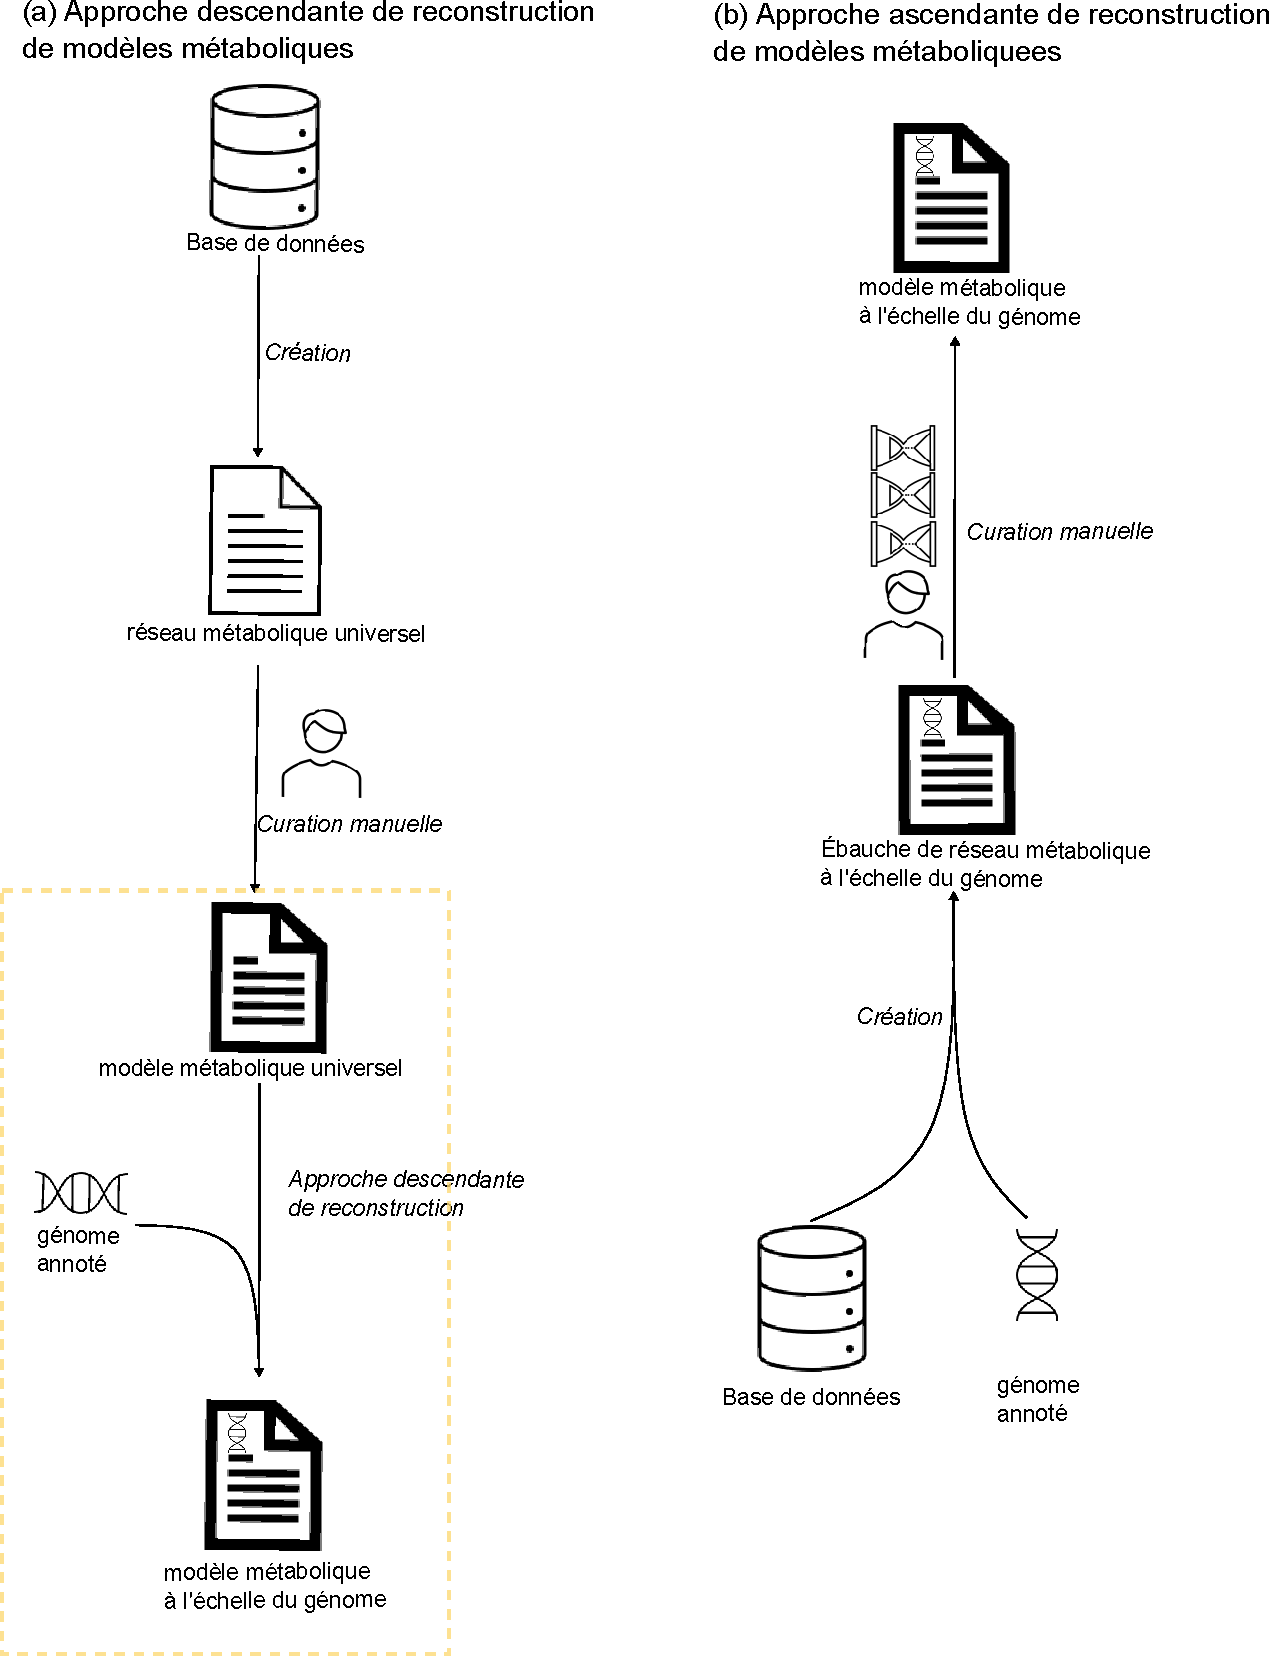
\includegraphics[width=\textwidth]{img/EDLA/approche-bottom-up-top-down.pdf}
    \caption{Illustration des approches descendante (a) et ascendante (b) pour reconstruire des modèles métaboliques à l'échelle du génome fonctionnels. En (a), la partie de curation manuelle n'est pas prise en compte dans l'approche de reconstruction, ce qui n'est pas le cas de l'approche ascendante (b). \maxime{texte trop petit ?} }
    \label{fig:approche-reconstruction}
\end{figure}



\subsubsection*{Diffusion et qualité des réseaux métabolique}
On peut voir qu'il existe plusieurs outils permettant de reconstruire le métabolisme. Cependant, standardiser sa représentation n'est pas encore acquis par la communauté scientifique \citep{Stobbe2014}. En effet, chaque base de données possède les fichiers de sortie différents permettant la représentation de la connaissance du métabolisme. On peut retrouver par exemple, BioCyc \citep{Karp2018} qui utilise des fichiers plats PGDB, le format BioPAX \citep{Demir2010} ou encore SBML\citep{Hucka2019}. La base de données KEGG \citep{Kanehisa} utilise d'autres fichiers plats et sa propre façon de représenter le métabolisme : KEGG Markup Language. Même si le choix syntaxique utilisé n'est pas commun à touts, nous retrouvons majoritairement le format SBML pour Systeme Biology Markup Language \citep{Hucka2019}, qui permet de représenter les voies de signalisation mais également, des paramètres mathématiques utiles pour la modélisation.

Concernant l'évaluation de la qualité du réseaux métabolique, au delà de l'objectif même de l'utilisateur ou de l'utilisatrice, il existe MEMOTE \citep{Lieven.2020} capable de vérifier la consistance du réseau métabolique en terme du nombre de gènes associés à des réactions, le nombre de réactions non associées à au moins un gène ou encore le nombre de métabolites qui ne sont jamais consommés mais produits, et donc, étant en accumulation dans le système. Le score évaluant la qualité du réseau est borné par la méthode de reconstruction choisie \citep{Lieven.2020}.


\subsection{Représentations mathématiques et informatiques du métabolisme}
Le métabolisme peut se représenter de deux grandes façons : sous forme d'un hypergraphe dirigé simple ou bipartite \citep{Belcour.2020}, ou sous forme d'une matrice st\oe{}chiométrique. La représentation sous forme d'un graphe informe sur les liens entre les réactions et métabolites d'un système biologique plutôt que sur la quantité de métabolites produits et/ou consommé associée davantage à la matrice st\oe{}chiométrique. Nous allons prendre l'exemple d'une voie de production connue, la glycolyse, chez une espèce lactique : \textit{Lactiplantibacillus plantarum}\\

Représentation simplifiée de la glycolyse chez \textit{Lactiplantibacillus plantarum}:\\
( HEX1 ) : $1\text{ glucose} \rightarrow 1\text{ glucose-6-phosphate}$\\
( PGI ) : $1\text{ glucose-6-phosphate} \leftrightarrow 1\text{ fructose-6-phosphate} $\\
( PFK ) : $1\text{ fructose-6-phosphate} \rightarrow 1\text{ D-Fructose 1,6-bisphosphate}$  \\
( FBA ) : $1\text{ D-Fructose 1,6-bisphosphate} \leftrightarrow 1\text{ Dihydroxyacetone phosphate}$\\$ + 1\text{ Glyceraldehyde 3-phosphate} $\\
( GAPD ) : $1\text{ Glyceraldehyde 3-phosphate}  \leftrightarrow 1\text{ 3-Phospho-D-glyceroyl phosphate} $\\
( PGK ) : $1\text{ 3-Phospho-D-glycerate} \leftrightarrow 1\text{ 3-Phospho-D-glyceroyl phosphate} $\\
( PGM ) : $1\text{ 3-Phospho-D-glycerate} \leftrightarrow  1\text{ 2-Phospho-D-glycerate} $\\
( ENO ) : $1\text{ 2-Phospho-D-glycerate} \leftrightarrow 1\text{ Phosphoenolpyruvate} $\\
( PYK ) : $1\text{ Phosphoenolpyruvate} \rightarrow 1\text{ pyruvate}$ \\

où $\text{HEX1}$, $\text{PGI}$, $\text{PFK}$, $\text{FBA}$, $\text{GAPD}$, $\text{PGK}$, $\text{PGM}$, $\text{ENO}$, $\text{PYK}$ sont les ensembles de réactions et où $\text{glucose}$, $\text{glucose-6-phosphate}$, $\text{fructose-6-phosphate}$, $\text{D-Fructose 1,6-bisphosphate}$, $\text{Dihydroxyacetone phosphate}$, $\text{Glyceraldehyde 3-phosphate}$, $\text{3-Phospho-D-glyceroyl phosphate}$, $\text{3-Phospho-D-glycerate}$, $\text{2-Phospho-D-glycerate}$, $\text{Phosphoenolpyruvate}$ et $\text{ pyruvate}$ sont les ensembles de métabolites principaux constituants la glycolyse de \textit{Lactiplantibacillus plantarum}.


\subsubsection{Matrice st\oe{}chiométrique}
Le métabolisme peut-être représenté sous forme d'une matrice st\oe{}chiométrique dont l'ensemble des réactions et des métabolites du système constituent respectivement les colonnes et les lignes. Le nombre à l'intérieur de la matrice représente le coefficient st\oe{}chiométrique de la réaction biochimique. Ainsi, la glycolyse chez \textit{Lactiplantibacillus plantarum} est représentée par la matrice st\oe{}chiométrique  suivante: 

\renewcommand{\kbldelim}{(}% Left delimiter
\renewcommand{\kbrdelim}{)}% Right delimiter
\[
  \kbordermatrix{
     & \text{HEX1} & \text{PGI} & \text{PFK} & \text{FBA} & \text{GAPD} & \text{PGK} & \text{PGM} & \text{ENO} & \text{PYK} \\
    \text{glucose}                                           & -1 & 0 & 0 & 0 & 0 & 0 & 0 & 0 & 0 \\
    \text{glucose-6-phosphate}                      & 1 & -1 & 0 & 0 & 0 & 0 & 0& 0 & 0 \\
    \text{fructose-6-phosphate}                      & 0 & 1 & -1 & 0 & 0 & 0 & 0& 0 & 0  \\
    \text{D-Fructose 1,6-bisphosphate}          & 0 & 0 & 1 & -1& 0 & 0 & 0& 0 & 0  \\
    \text{Dihydroxyacetone phosphate}         & 0 & 0 & 0 & 1 & -1 & 0 & 0& 0 & 0  \\
    \text{Glyceraldehyde 3-phosphate}         & 0 & 0 & 0 & 1 & -1 & 0 & 0& 0 & 0  \\
    \text{3-Phospho-D-glyceroyl phosphate} & 0 & 0 & 0 & 0 & 1 & -1 & 0& 0 & 0  \\
    \text{3-Phospho-D-glycerate}                   & 0 & 0 & 0 & 0 & 0 & 1 & -1& 0 & 0 \\
    \text{2-Phospho-D-glycerate}                  & 0 & 0 & 0 & 0 & 0 & 0 & 1& -1 & 0  \\
    \text{Phosphoenolpyruvate}                    & 0 & 0 & 0 & 0 & 0 & 0 & 0& 1 & -1  \\
    \text{ pyruvate}                                         & 0 & 0 & 0 & 0 & 0 & 0 & 0& 0 & 1 \\
    }
\]


\subsubsection{Graphe}
Pour représenter des réseaux métaboliques, un graphe bipartite dirigé pondéré est souvent privilégié \citep{Barabasi2004}. Le graphe est alors composé de deux types de sommets, un pour les métabolites et un pour les réactions, et d'arcs symbolisant les relations "être produit par" ou "être consommé par" entre les métabolites et les réactions. Mathématiquement, il peut être exprimé ainsi : soit un graphe bipartite G définit comme un tuple $\gmodel = \langle M, R, E \rangle$ où $R$, $M$ et $E$ représentent les ensembles respectifs de réactions, de métabolites et des arcs reliant les métabolites aux réactions. Un réactant $m$ consommé par la réaction $r$ est définie comme $e = \langle m,r \rangle$, et un produit $m$ de la réaction $r$ est définie comme suit $e = \langle m,r \rangle$ où $m\in M$ et $r\in R $.

Une représentation de la glycolyse de \textit{Lactiplantibacillus plantarum} sous forme d'un graphe bipartite est illustrée dans la figure \ref{fig:graph-network}, où les carrés représentent les réactions et les cercles représentes les métabolites.


\begin{figure}[h!]
    \centering
    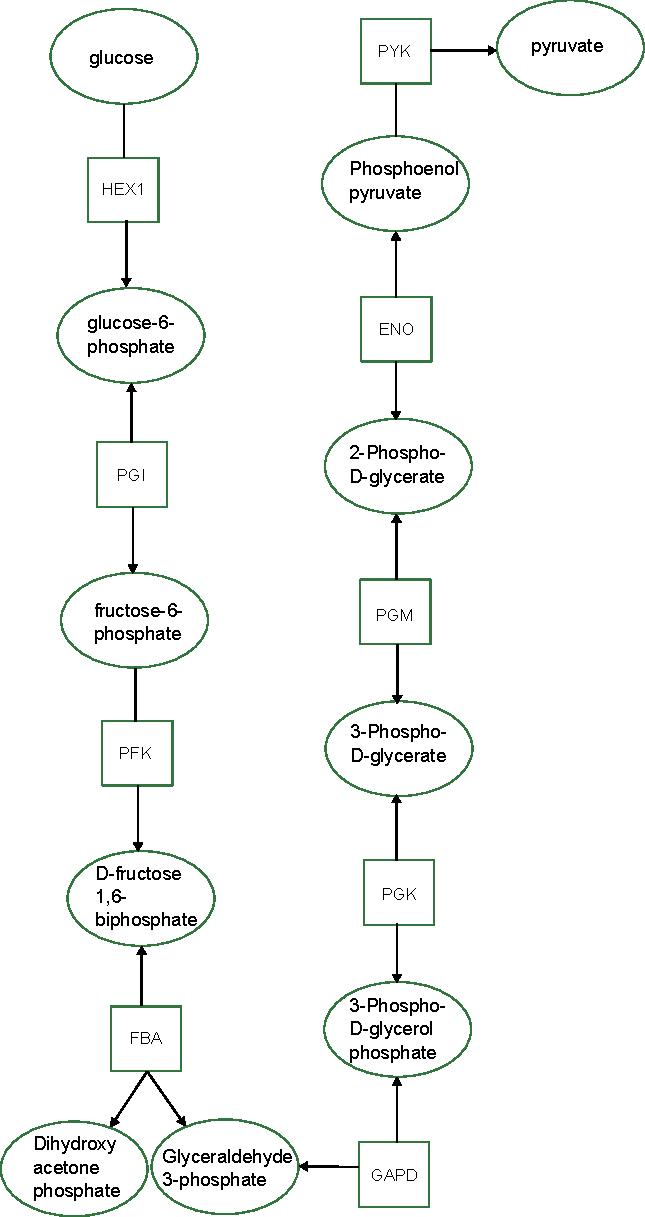
\includegraphics[width=0.6\textwidth]{img/EDLA/graph_network.pdf}
    \caption{Représentation du métabolisme sous forme d'un graphe bi-partite. Les carrés sont associés aux réactions, les cercles aux métabolites et les arcs représentent les relations de consommation et de production des métabolites.}
    \label{fig:graph-network}
\end{figure}


\subsection{Analyse structurelle de réseaux métaboliques}
Avant d'aborder les processus de modélisation de réseaux métaboliques, une étude de la structure de réseaux métaboliques peut-être fait au moyen d'algorithme de la théorie des graphes. Dans un graphe non orienté, seule la structure du réseau peut être analysée et comparée. La topologie peut se faire à l'échelle des substrats uniquement \citep{Jeong2011} ou des réactions uniquement \citep{Wagner2001}. La comparaison de réseaux nous permet d'identifier des différences fonctionnelles, de détecter des variations entre souches d'une même espèces ou encore, de formuler des hypothèses de capacité biosynthétiques entre les organismes, sans prendre en compte les interactions entre elles \citep{Biggs2015}. En effet, dans \citep{Ay2012}, les auteurs et autrices utilisent une technique d'alignement de réseaux métabolique pour identifier des motifs communs conservés entre plusieurs organismes. Dans un réseau complexe, représenter la connectivité d'un substrat est très massivement utilisé par la communauté scientifique \citep{Ma2003}, cependant, les co-facteurs tels que ATP, ADP etc sont sur représentés ce qui rend fastidieux l'analyse par les biologistes \citep{Sweetlove2005}. En revanche, identifier des composés fortement connectés permettent de montrer des propriétés de robustesse d'un réseau métabolique face à des délétions enzymatiques: un grand nombre de délétion engendre peu de perturbations métaboliques  \citep{Lemke2004}. La comparaison topologique permet en somme d'effectuer une comparaison structurelle entre organisme \citep{Ma2003} ou encore, de trouver le nombre moyen de plus petit chemins\citep{Wagner2001} dans un organisme.\\ 


Comparer la structure de réseaux métaboliques est purement qualitatif mais permet de souligner des hypothèses sur ce que chaque réseau métabolique pourrait être capable de produire et de consommer. Pour vérifier ces hypothèses, on utilise la modélisation du métabolisme qui, à partir d'un environnement nutritionnel, vise à inférer les ensembles de réactions activées et métabolites produits. Au moyen d'approches numériques et qualitatives, des hypothèses testables en laboratoire sur différents systèmes biologiques peuvent être générées et de nouvelles connaissances peuvent être prédites. De plus, l'élaboration de tels modèles métaboliques permet l'intégration de diverses données omiques, affinant ainsi les prédictions \citep{Passi2022}.


\newpage

\section{Modélisation métabolique à l'échelle d'un génome}
Pour rappel, la modélisation du métabolisme permet d'effectuer des simulations en utilisant le réseau métabolique. Cette approche se fait au moyen d'un modèle métabolique capable de prédictions et pouvant être contraint par des données multi-omiques. On peut trouver dans la littérature de nombreuses méthodes d'analyse du métabolisme, aussi bien à l'échelle d'une voie métabolique particulière qu'à l'échelle d'une communauté bactérienne composée de plusieurs centaines de bactéries, se basant sur divers formalismes mathématiques : numérique, logique ou hybride. Une revue des méthodes d'analyse des modèles métaboliques à l'échelle d'un génome est proposée dans les paragraphes suivants. 

\subsection{Méthodes numériques d'un réseau métabolique}
La modélisation numérique du métabolisme informe quantitativement sur des mécanismes biologiques intracellulaires d'une espèce en se basant sur la matrice st\oe{}chiométrique ou bien sur les données cinétiques. 


\subsubsection{Constantes cinétiques des réactions}
Les réactions biochimiques consomment des substrats et produisent des produits à une vitesse cinétique $k$ selon la réaction globale suivante:
\[
\text{substrats} \overset{k}{\rightarrow} \text{produits} 
\]

Il existe des modèles cinétiques se basant sur des constantes cinétiques et des équations du type Michaelis-Menten qui intègrent la constante d'affinité des enzymes pour leur substrat \citep{costaKineticModelingCell2016}. Soit $E$, $S$, $ES$, $P$ des substrats, $k_1$, $k_{-1}$ et $k_{cat}$ des constantes cinétiques, le schéma réactionnel global peut être décrit comme suit:

\begin{center}
\ce{{E} + {S}
<=>[k_1][k_{-1}]
\ce{ES}
->[k_{cat}]
\ce{E} + {P}
}\\
\end{center}

De ce schéma, l'équation de Michaelis-Menten permet de calculer la vitesse d'une réaction:
\begin{equation}
    V = \frac{V_{max}[S]}{K_m + [S]} \label{1}
\end{equation}
dans laquelle $V_{max}[S]$ correspond à la vitesse maximal de transformation d'un substrat $V_{max}$ multiplé par la concentration du substrat $[S]$ et  $K_m$ représente la constante d'affinité. 

L'avantage des modèles cinétiques est qu'ils assurent un haut niveau de confiance sur les prédictions de par l'inférence des paramètres cinétiques. En revanche, acquérir ces données peut-être coûteux en temps et limite leur utilisation à des réseaux métaboliques plus petits (généralement de l'ordre de la vingtaine de réactions) \citep{vanrosmalenModelReductionGenomescale2021}.


\subsubsection{Contraintes numériques}
Avec les avancées des technologies à haut débit, des méthodes computationnelles se sont développées pour analyser ces données. Parmi elles, les méthodes de modélisation basées sur contraintes y contribuent en considérant des contraintes liées au réseau métabolique: topologiques, thermodynamiques et enzymatiques \citep{Rajvanshi2013}.
%
%Les méthodes basées sur des contraintes permettent de trouver mathématiquement une solution en se basant sur des limites d'un espace de recherche. Ainsi, toutes les variables qui partagent les mêmes contraintes seront présentes dans le même espace de recherche définit en amont. Ce type d'approches se base sur des techniques d'optimisations maximisant ou minimisant une fonction objective.

Parmi les méthodes sous contraintes, on retrouve les méthodes d'analyse par équilibre des flux (FBA, de l'\textit{anglais}, \textit{Flux balance analysis})\citep{Orth2010}. Son objectif est de calculer les flux de consommation et de production de métabolites pour chaque réaction qui compose le système. Pour cela, le système doit satisfaire une contrainte thermodynamique: loi de conservation de la masse. Cette loi définie l'équilibre d'un système réactionnel et se lit de la façon suivante:

\begin{equation}
\label{conservation-masse}
\frac{d\text{[x]}}{dt} = \text{S.v}
\end{equation}

dans lequel, S représente la matrice st\oe{}chiométrique, v le vecteur de flux des composés des réactions et $\frac{d\text{[x]}}{dt}$ la variation de la concentration du composé x au cours du temps $t$. \\

À l'état stable du système, on n'observe aucune accumulation de métabolites à l'intérieur du système, c'est à dire, que pour un même métabolite $m_i$ intracellulaire, la quantité de $m_i$ produite est égale à la quantité de $m_i$ consommée. Le flux de chaque réaction, i.e. l'approximation de la vitesse cinétique, est ajustée de façon à ce qu'il n'y ait pas d'accumulation dans le milieu intracellulaire. Ainsi, dans l'équation \ref{conservation-masse}, la concentration du métabolite x ne varie pas au cours du temps et l'équation sous hypothèse d'état stable s'écrit de la façon suivante: 

\begin{equation}
\text{S.v}_{int} = 0
\end{equation}

Cette hypothèse forte est justifiable car la vitesse des réactions intracellulaires est plus rapide que les changements macroscopiques observables, par exemple, la croissance d'une plante \maxime{ref}.\\

Lors de la résolution d'un problème FBA, une fonction objective est optimisée, soit en la maximisant soit en la minimisant. Généralement, la fonction objective est une réaction de biomasse simulant la croissance d'un organisme en fonction des substrats disponibles \maxime{ref dans papier FEIST2010344}. Cette optimisation redirige les flux des métabolites à l'intérieur de la cellule pour permettre une production de biomasse. La conception d'une telle  fonction n'est pas un processus trivial, d'autant plus que chaque espèce ne pousse pas à la même vitesse \maxime{ref}. En revanche, nous retrouvons des familles de composés en commun\citep{FEIST2010344}. \\ 

Dans un réseau métabolique réaliste, il y a plus de réactions que de métabolites et donc, pour un même métabolite, il existe plusieurs chemins possibles le dégradant. Ainsi, lors de l'étape d'optimisation de la fonction objective, la méthode de flux FBA ne peut donner une solution unique de flux (voir Figure \ref{cone-solution}). 

Afin de restreindre l'espace de recherche par le solveur, les valeurs possibles de flux sont bornées par un flux minimal $v_{i_{min}}$ et maximal $v_{i_{min}}$, de la façon suivante:

\begin{equation}
 \text{$v_{i_{min}}$} \leq v_i \leq \text{$v_{i_{max}}$}
\end{equation}

Toutes ces contraintes se traduisent sous le programme linéaire global suivant:

\begin{align}
\begin{split}
\label{lineaire}
    \text{maximiser/minimiser }\text{$f_{obj}$} \\
    \text{tel que } (S.v)_{int} = 0\\
    \text{et } \text{$v_{i_{min}}$} \leq v_i \leq \text{$v_{i_{max}}$}
\end{split}
\end{align}

où $f_{obj}$ est la fonction objective, $(S.v)_{int} = 0$ suppose l'état stable du système et $v_{i_{min}}$ $\leq$ $v_i$ $\leq$ $v_{i_{max}}$ les valeurs de flux inférieures et supérieures. \citep{Orth2010}\\

Soit un réseau métabolique composé de 2 réactions donc celle de la réaction de biomasse. Après optimisation de la réaction de biomasse, deux optima sont trouvés (un seul sera choisi après n itérations) (voir Figure \ref{fig:cone-solution}). Biologiquement, cela signifie qu'il existe un ensemble de valeur de flux possibles pour la seconde réaction garantissant une croissance optimal. Ces ensembles de valeurs sont déterminables par une méthode décrite dans les paragraphe ci-dessous.

L'approche FBA constitue la base des méthodes de modélisation du métabolisme par contraintes. Dans les prochains paragraphes, une liste non exhaustives des variantes du FBA couramment utilisées dans la littérature sera présentée.


\paragraph*{Analyse parcimonieuse par équilibre des flux}
Une des variantes de l'analyse par équilibre des flux permettant d'effectuer des analyses complémentaire est l'analyse parcimonieuse par équilibre de flux  (pFBA) \citep{Lewis2010}. Elle vise à trouver une unique solution en minimisant la somme totale des flux impliqués dans l'optimisation de la fonction objective, tout en maintenant un flux optimal de croissance.

\paragraph*{Analyse de la variabilité des flux}
L'analyse de la variabilité des flux (FVA) \citep{Mahadevan2003}, évalue pour chaque réaction, les valeurs de flux possibles. En effet le FBA trouve une distribution de flux non unique satisfaisant les contraintes du problème linéaire \eqref{lineaire}. Le FVA permet ainsi d'identifier des \textit{réactions bloquées}, \textit{i.e.} pour lesquelles cette réaction n'admettra pas de flux; les \textit{réactions essentielles}, \textit{i.e.} pour lesquelles un flux non nul est toujours présent, et les \textit{réactions alternatives}, \textit{i.e.} pour lesquelles il existe une distribution de flux où ces réactions ne sont pas activées.


\begin{figure}[h!]
    \centering
    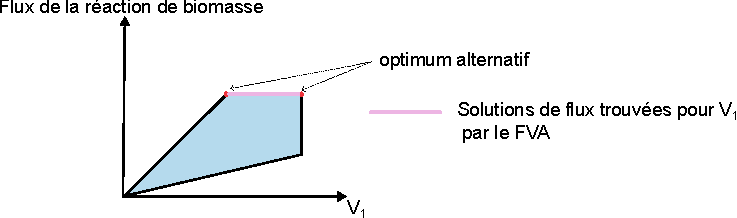
\includegraphics[width=1\textwidth]{img/EDLA/cone-solution.pdf}
    \caption{\textbf{Cône de solution obtenu lors de la résolution d'un FBA.}}
    \label{fig:cone-solution}
\end{figure}


\paragraph*{Analyse par équilibre des ressources}
Une extension du problème d'optimisation énoncé plus haut permettant de prendre en compte la machinerie de production des protéines se fait grâce à l'analyse par équilibre des ressources (RBA) \citep{Goelzer2015}. Dans ce dernier cas, chaque cellule utilise les ressources internes de façon économique.

\paragraph*{Analyse par équilibre dynamique des flux}
Ces méthodes peuvent être utilisées dynamiquement grâce à un processus itératif : analyse par équilibre dynamique de flux (dFBA) \citep{Mahadevan2002}. Le processus dynamique se modélise à l'aide d'un système d'équations différentielles ordinaires (ODE).  En plus de la dimension temporelle, la spatialisation peut également être modélisée avec des ODE, PDE (équations différentielles partielles) \citep{Succurro} ou encore avec un dFBA avec l'outil COMETS \citep{Harcombe2014}. A chaque pas de temps $\delta t$, défini manuellement, le taux de croissance de chaque espèce et les concentrations des composés à suivre sont calculées grâce à la résolution d'un FBA. 

\paragraph*{Analyse des mode de flux élémentaires}
Les modes de flux élémentaires ou \textit{elementary flux mode} en \textit{anglais} (EFM), sont les ensembles minimaux de réactions activées respectant la réversibilité des réactions qui garantissent l'état stationnaire du système\citep{SCHUSTER1994, Trinh2009}. Cette méthode permet principalement d'identifier des voies métaboliques optimales pour la production de composés ou encore d'évaluer la robustesse du réseaux, c'est à dire, sa capacité à répondre à des changement de structure \citep{Klamt2002}. Une des limites de cette méthodes est que le nombre de modes élémentaires augmente rapidement, devenant impossible à générer pour des réseaux à l'échelle du génome. Plus récemment, une méthode combinant la programmation par ensemble de réponse (ASP, de l'\textit{anglais, answer set programming} paradigme logique adapté à la résolution de problèmes combinatoires \citep{Lifschitz2008}, et les EFM sont utilisés sur le c\oe{}ur du métabolisme de \textit{E. coli} permettant de réduire le coût calculatoire en intégrant différentes contraintes linéaires \citep{Mahout2020}.


\subsubsection{Intégration de données multi-omiques}
Ces méthodes d'optimisation sous contraintes permettent de mettre en évidence des interactions entre bactéries, ou révèlent des activations/ inhibition de voies métaboliques de la communauté. Des méthodes d'intégration de données multi-omiques utilisent principalement les données métatranscriptomiques, en ajoutant des contraintes linéaires et donnent des informations  supplémentaires sur différents processus de régulation (activation/inhibition). Une liste non exhaustive est présentée ci-dessous permettant l'intégration de ces données : GIMME \citep{Becker2008}, crée un modèle métabolique cohérent avec les données biologiques et la fonction objective à maximiser, en minimisant les réactions trouvées inactives par l'outil. INIT \citep{Agren2012} maximise l'utilisation des réactions basées sur un score de confiance et minimise les réactions sans protéine associée.  INIT peut intégrer à la fois des données transcriptomique ou protéomiques. Enfin, plus récemment, RIPTiDe \citep{Jenior2020} utilise une approche parcimonieuse afin d'identifier les solutions les plus efficaces en termes de coûts, reflétant ainsi au mieux la transcription de la cellule.

\newpage

\subsection{Méthodes qualitatives d'analyse d'un réseau métabolique}
La modélisation qualitative du métabolisme vise l'émergence de propriétés topologiques et fonctionnelles globales \citep{Steuer2007}. Dans les paragraphes suivants, les méthodes qualitatives pour analyser un réseau métabolique seront présentées.

\subsubsection{Résolution de problèmes SAT et SAT dérivés }

\subsubsection{Graphes}
A partir d'un graphe, des propriétés topologiques comme la modularité \citep{Holme2011} ou la centralité \citep{Kim2019} sont souvent utilisées en biologie des systèmes. La modularité d'un réseau est sa capacité à être décomposable en sous graphe densément connecté mais faiblement relié entre eux. La centralité d'un n\oe{}ud est un indice qui capture l'importance de ce n\oe{}ud dans le graphe. D'autres méthodes se basent sur la détection de motifs où pour chaque occurrence du motif, un sous graphe est généré \citep{Lacroix2006}. Plus récemment, une approche basé sur les graphes à été utilisé pour détecter des EFM et une comparaison des outils numériques est faite \citep{Arabzadeh2018}. En plus de ces analyses, certains auteurs et autrices se concentrent sur l'identification de voies métaboliques à partir d'un ensemble de métabolites sources et/ou de métabolites cibles \citep{Heiden2002}. Kuffner \citep{kuffner2000} et ses collègues démontrent que l'analyse des chemins métaboliques à partir d'une paire source-cible est un non sens biologique. En énumérant l'ensemble des chemins possibles permettant d'aller du glucose au pyruvate, plus de 500 000 voies métaboliques ont été trouvées. Une autre approche consiste à utiliser les données  \textit{a priori} comme par exemple les données d'expression de gènes, pour contraindre les voies métaboliques \citep{Zien2000}. Enfin, dans \citep{Simeonidis2003} les auteurs utilise une analyse du plus court chemin entre deux molécules enzymatiques. Ils comparent avec les distances des deux gènes associés et démontrent qu'il n'existe pas de lien entre les deux. Cela suggére qu'il existe un mécanisme d'évolution de voies métaboliques. Dans une approche différente, NetSeed propose de trouver un ensemble de graines possibles en se basant à la fois sur le calcul de composantes fortement connexes (SCC) et sur le concept de l'écologie inversée \citep{Carr2012}.
 
\subsubsection{Problème SAT}
Un problème satisfiable (SAT) est utilisé pour déterminer si une formule booléenne peut être est satisfiable par un ensemble de valeur. Par exemple, pour que la proposition booléenne \ref{unsat} soit vraie, il faut que la valeur que l'on assigne à $x_1$ soit différente d'elle même. Ainsi, aucune valeur ne peut être assignée à $x_1$ qui puisse vérifier l'expression booléenne et donc, cette proposition logique n'est pas satisfiable. 


\begin{align}
\label{unsat}
    x_1 \land \neg x_1
\end{align}

En revanche, l'expression booléenne \ref{sat} stipule qu'il faut que la variable $x_1$ soit différent de $x_2$. Il existe un nombre infini de solution comme $x_1 = 1$ et $x_2 = 0$ qui satisfont le problème logique, ce problème est donc SAT.

\begin{align}
\label{sat}
    x_1 \land \neg x_2
\end{align}


\paragraph*{Paradigme logique par ensemble de réponse (ASP)}
Ce paradigme est logique est une forme de programmation déclarative utilisée pour des résoudre des problèmes combinatoires \citep{Lifschitz2008}. L'ASP décrit les problèmes sous forme de règles, de contraintes et de faits logiques. Il est composé de 3 structures: une tête, un corps et un séparateur ($:-$). Par exemple, la proposition \ref{exemple1} dit: "\textit{X vole si X est un oiseau et X n'est pas une autruche}". Après éxécution du programme, seul la réponse \texttt{vole(toto)} satsfait l'ensembles des règles et contraintes.

\begin{lstlisting}[mathescape=True,label={exemple1},caption={Code ASP permettant de calculer le scope métabolique},captionpos=b]
    	oiseau(toto).  % faits
    	autruche(titi). % faits
    	vole(X) :- oiseau(X); not autruche(X).
\end{lstlisting}

En revanche, Aune solution n'est possible pour la proposition \ref{exemple2}, puisque toto est à la fois un oiseau et une autruche.

\begin{lstlisting}[mathescape=True,label={exemple2},caption={Code ASP permettant de calculer le scope métabolique},captionpos=b]
    	oiseau(toto).  % faits 
    	autruche(toto).  % faits
    	vole(X) :- oiseau(X); not autruche(X).
\end{lstlisting}

Lors de sa résolution, le système \texttt{clingo} va instancier les règles décrite en ASP sous forme de variables (étape de \textit{grounding} avec \texttt{gringo}) puis le solveur \texttt{clasp} applique les différentes contraintes aux modèles afin de sélectionner le ou les modèles stables, c'est à dire, satisfaisant l'ensemble des règles et contraintes. Ces modèles stables sont issus directement des règles logiques, permettant aux utilisateurs et utilisatrices d'obtenir une explication du résultat. Le schéma global du processus de résolution de problèmes en ASP est récapitulé dans la figure \ref{fig:asp}.

\begin{figure}[h!]
    \centering
    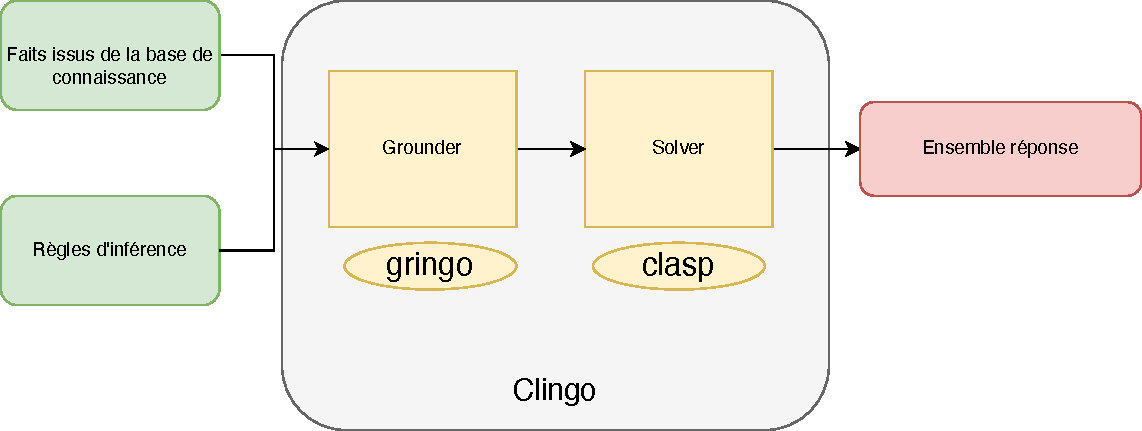
\includegraphics[width=1\textwidth]{img/EDLA/fonctionnement_ASP}
    \caption{Schéma récapitulant les étapes de résolution d'un problème ASP à partir des régles logiques.}
    \label{fig:asp}
\end{figure}

\subsubsection{Application à des problèmes biologiques}

Des méthodes basées sur des problèmes SAT sont appliqués à l'étude du métabolisme. Nous retrouvons les travaux de \citep{Collet2013} etendant le réseau métabolique de \textit{Ectocarpus Siliculosus} en implémentant la possibilité d'ajouter des réactions réversibles. \citep{Prigent2017} se base la même méthode dérivée de résolution SAT, le paradigme logique par ensemble de réponse (ASP) en créant un outil de complétion de réseaux métabolique, Meneco, qui ajoutte des réactions considérées comme essentielles. Les travaux de \citep{Tiwari2007} ont proposé une méthode SAT pour analyser des réseaux de réactions ou encore \citep{Corblin2006} qui appliquent une méthode basée sur SAT pour déchiffrer des réseaux de régulation de gènes.\\

A l'échelle d'un génome, des travaux ont couplé l'ASP avec l'algorithme d'expansion de réseaux métaboliques \citep{Ebenhoh2004} décrivant la notion de productibilité d'un métabolite \citep{Frioux2018,Aite2018}. Ces derniers ont inféré cet algorithme sous forme d'un raisonnement logique \citep{Levesque1986} en créant les règles correspondantes. Ainsi, un composé est productible par une réaction si l'ensemble des réactants de cette réaction est également productible. Cette règle récursive est implémenté en ASP par la proposition \ref{recursive}.

\begin{lstlisting}[mathescape=True,label={recursive},caption={Code ASP permettant de calculer le scope métabolique},captionpos=b]
productibilite(Compose) :- graine(Compose).

productibilite(Compose) :- produit(Compose,Reaction); 
      reaction(Reaction); 
      productibilite(Compose2) : reactant(Compose2,Reaction).
\end{lstlisting}

%\begin{flalign*}
%\label{recursive}
%& productibilit\acute{e}(Compos\acute{e}) :- graine(Compos\acute{e}).& 
%\end{flalign*}
%\begin{equation}
%\begin{split}	
% 	productibilit\acute{e}(Compos\acute{e}) :-  & produit(Compos\acute{e},Reaction), \\
%    & reaction(Reaction) \\
%    & productibilit\acute{e}(new\_Compos\acute{e}) : reactant(new\_compos\acute{e},Reaction).
%\end{split}
%\end{equation}

Au sein de la proposition \ref{recursive}, il y a tout d'abord une étape d'initialisation, informant que les gaines, c'est à dire le milieu nutritionnel est déjà productible, puis la partie récursive. \\

Afin de générer des règles, il faut une base de connaissance adéquate, c'est à dire, l'ensemble des faits nécessaires qui décrit, dans notre cas, le réseau métabolique. Dans le cas de la proposition \ref{recursive} décrivant la productibilité d'un composé, la base de connaissance est constituée de l'ensemble du milieu de culture représenté par l'atome \texttt{graine} ,  des réactions (\texttt{reaction}), des réactants (\texttt{reactant}) et des produits (\texttt{produit}).


\subsection{Défis rencontrés lors de la modélisation qualitative et numérique d'une cellule}
\label{defi}
Pour analyser une cellule du point de vue du métabolisme, des choix de modélisation doivent être pris en compte. Tout d'abord, les réactions de transports permettant le passage de métabolites du milieu intracellulaire au milieu extracellulaire. Pour les deux types de modélisation, des réactions de transports doivent être ajoutées aux modèles métaboliques prenant en compte les différents éléments du milieu de culture. Un second défi rencontré est la prise en compte des cycles de régénrération des co-facteurs, \textit{e.g.}. NADH, NADPH, FADH, etc. Avec une approche par raisonnement, ils sont considérés comme disponibles car ils sont dépendants de ces cylcles complexes et potentiellement thermodynamiquement non faisable. Avec les méthodes FBA, les contraintes font converger les flux de métabolites  vers les voies thermodynamiquements faisables.\\


\subsection{Méthodes hybrides de modélisation à l'échelle d'un modèle métabolique}

La modélisation est dite hybride lorsqu'une variable rassemble différentes informations issues de formalismes mathématiques ou informatiques comme par exemple discret et continu \citep{Cruz2022}. Il existe trois grands types de modèle hybride : (i) indépendant, (ii) couplé ou (iii) imbriqué \citep{Stephanou2016}. Le modèle indépendant consiste en au moins deux modèles décrivant le même phénomène à des échelles de précision différentes et où aucune interaction entre les modèles existe. Le modèle couplé  consiste en au moins deux modèles pouvant communiquer unidirectionnellement ou bidirectionnellement entre eux. Enfin, le modèle hybride imbriqué forme une seule entité composés de sous-parties sensibles au changement du contexte, déclenché par un seuillage par exemple. Il ne sera pas détaillé dans cette section. \\
 
\subsubsection{Indépendants}
Au sein des modèles indépendants, c'est l'approche qui est qualifiée d'hybride et non le modèle en lui-même. Les réseaux métaboliques possèdent la propriété d'être décomposables \citep{Fisher2010}, c'est à dire qu'ils peuvent être décomposés en plusieurs petites structures qui sont plus simple et permettant une analyse facilitée. On peut imaginer une approche de reconstruction de réseaux métaboliques hybride, utilisant comme premier modèle une reconstruction bottom-up et de l'autre, une reconstruction top-down. Ce type d'approche est utile pour décrire un même phénomène à des échelles différentes permettant ainsi d'identifier lequel des modèles utilisés est le plus précis et le moins coûteux computationnellement. \\

\subsubsection{Couplé}
Dans le cadre des modèles couplés, les variables de sortie d'un modèle servent en entrée d'un autre. Ce type de modèle hybride sert principalement à traiter des problèmes à plusieurs échelles \citep{Brook2008}. Dans le cas des modèles hybrides appliqués à la biologie des systèmes, Frioux et al \citep{Frioux2019} ont développé une méthode de complétion de réseaux de métabolique hybride basé sur l'ASP. Le code ASP combine à la fois le solveur logique Clingo \citep{Gebser2019} et le solveur linéaire Clingo[LP] \citep{Janhunen2017} résolvant respectivement les contraintes logiques et linéaires du programme. Les modèles trouvés satisfont ainsi les contraintes linéaires et logiques. Dans le cas où les contraintes linéaires ne sont pas satisfaites, une communication bidirectionelle entre les deux solveurs a lieu informant de l'impossibilité à satisfaire les contraintes.\\

Toutes ces approches décrites permettent l'analyse d'un réseau métabolique à l'échelle d'un génome. Comme nous avons vu dans l'introduction, les données générées massivement sur des communautés non-cultiables entrainent le développement de modèles de communauté pour générer des hypothèses. Dans le reste de ce chapitre, des méthodes à l'échelle de l'écosystème analysant des communautés de microorganisme seront présentées, avec leurs avantages, leurs limites et leurs applications.


\section{Modélisation du métabolisme des écosystèmes microbiens}
Tout comme pour la section sur l'analyse du métabolisme à l'échelle du génome, les méthodes numériques seront d'abord présentées.

\subsection{Méthodes numériques appliquées à plusieurs réseaux métaboliques}

\subsubsection{Équations différentielles ordinaires (ODE)}
Un moyen pour décrire la dynamique spatio-temporelle d'une communauté microbienne est d'utiliser les équations différentielles \citep{Succurro}. In 1838, Verhulst a défini le premier modèle décrivant la croissance d'une bactérie dans une culture au cours du temps \citep{verhulst}. Par la suite, les modèles proies-predateurs ont été utilisés pour décrire une interaction, positive ou négative, d'une espèce prédatrice sur la croissance d'une autre en communauté \citep{Nair2019}. On peut également retrouver les modèles de Lokta et Volterra, largement utilisés pour étudier l'évolution dans le temps d'un écosystème et principalement, les modèles généralisés de Lokta-Volterra, prenant en compte les données d'abondance relative de bactéries lors d'une analyse en métagénomique \citep{Berry2014}. En revanche, ces modèles ne se basent que sur les interactions trophiques entre les bactéries et ne prennent pas en compte l'environnement nutritionnel. Il existe cependant une extension du modèle de Lokta-Volterra généralisé permettant de tenir compte d'une potentielle perturbation environnementale sur le comportement d'un individu \citep{Stein2013}.
Toutes ces méthodes sont malheureusement "data-driven", i.e. dépendantes des données et de la connaissance que l'on peut avoir sur le système biologique d'étude et ne sont pas mécanistique. Ainsi pour permettre une analyse détaillée du système biologique permettant de répondre aux questions, "qui produit quoi ?" ou "comment une perturbation dans la composition bactérienne ou dans les milieux nutritifs impacte la communauté bactérienne ?", il faut inférer cette connaissance sous forme de paramètres. En d'autres termes, chaque mécanisme de régulation que l'on souhaite modéliser doit être décrit par, \textit{a minima}, une équation. 

% \subsubsection{Intégration de données multi-omics dans la modélisation du métabolisme}
% La mise à disposition de plusieurs données omics sur un même système biologique permet d'en apprendre d'avantage sur ce qui est activé (transcriptomique), ce qui est produit (métabolomique) ou bien les vitesses de croissance bactérienne (cultures pures). \\
% Il existe des outils permettant d'intégrer les données de métatranscriptomiques en contraignant les réseaux métaboliques. 




\subsubsection{Analyse statique sous contraintes}
Les modèles basés sur les flux s'appliquent également à l'échelle de la communauté. Le modèle de communauté peut se décrire de trois façons possibles: compartimentalisé, soupe ou encore indépendant (voir Figure \ref{fig:community-type}) \citep{Colarusso2021}. Chaque modèle possède des propriétés propres \citep{Succurro2018}. Le modèle soupex@ (Figure \ref{fig:community-type}b) permet d'explorer le potentiel métabolique de la communauté sans la nécessité d'obtenir une résolution de chaque modèle individuel. Cela se traduit généralement par une optimisation d'une fonction de biomasse communautaire créée en assemblant les compositions de chaque fonction de biomasse des organismes. Le modèle indépendant comme le modèle compartimentalisé permettent de prendre en compte les abondance de chaque individu. Dans le modèle compartimentalisé \ref{fig:community-type}a), chaque bactérie possède son propre espace intracellulaire et extracellulaire, permettant ainsi des échanges entre espèces. Un espace extracellulaire les englobe contenant le milieu nutritionnel. La fonction de biomasse communautaire correspond généralement à la somme des valeurs de flux de biomasse individuel. Dans un modèle indépendant (Figure \ref{fig:community-type}c), chaque bactérie conserve son propre espace intracellulaire mais partagent le même espace extracellulaire. La fonction de biomasse communautaire peut-être soit multi-objective soit à l'echelle de chaque individu, comme pour le modèle compartimentalisé. 


\begin{figure} [h!]
    \centering
    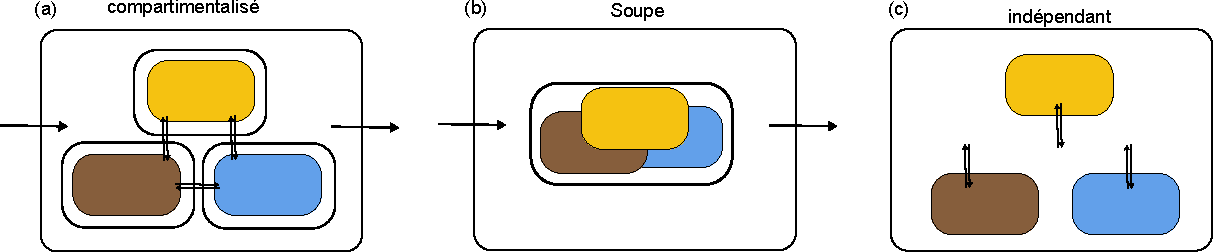
\includegraphics[width=\textwidth]{img/EDLA/community_strategies.pdf}
    \caption{Différents types de stratégies pour construire un modèle de communauté. (a) Dans le modèle compartimentalisé, chaque bactérie possède son propre compartiment cytosolique et extracellulaire. Un compartiment extracellulaire commun à l'ensemble des bactéries est également disponible. (b) Dans le modèle soupe, les bactéries sont assemblées en une seul pour former un supra-organisme. (c) Les bactéries ont chacun leur propre compartiment cytosolique mais partagent un milieu extracellulaire commun.}
    \label{fig:community-type}
\end{figure}


En fonction du type de représentation du modèle de communauté il existe plusieurs outils de modélisation de communautés microbiennes \citep{Colarusso2021}. Dans Henry et al \citep{Henry2016}, les auteurs ont choisi de maximiser une fonction de biomasse communautaire se basant sur la composition des réactions de biomasse de chaque taxon présent dans la communauté. Microbiome modeling toolbox \citep{Baldini2019}, MiCOM \citep{diener2020} et SteadyCom \citep{Chan2017} maximisent tous la somme des flux de la fonction de biomasse de chaque organisme et permettent l'étude de plus grandes communautés.  cFBA \citep{Khandelwal2013} ou encore Koch et al, \citep{Koch2016} permettent une analyse sur de petites communautés. Enfin, dans la catégorie d'une optimisation à plusieurs niveaux, on peut retrouver les outils suivants : OptCom \citep{Zomorrodi2012}, NECom \citep{Cai2020}, maximisant les fonctions de biomasse de chaque modèle individuel puis les flux de production de biomasse à l'échelle de la communauté. Pour des raisons de coût calculatoire, appliquer ces outils sur des grandes communautés microbiennes est non réalisable. \\

Toutes ces méthodes basées sur des contraintes permettent d'étudier le métabolisme et par conséquent peuvent être utilisées pour mettre en évidence l'impact positif (coopération) ou négatif (compétition) d'une interaction bactérienne. En effet, dans \citep{Freilich2011} les scores de potentiels de coopération et de compétition sont inférés en caractérisant les relations de donneurs-receveurs et de gagnants-perdants au sein de l'écosystème. Plus récemment, MMinte \citep{Mendes-Soares2016} prédit l'impact positif ou négatif d'une espèce sur une autre en comparant les croissances des espèces seules et lorsqu'elles sont en interactions deux à deux. L'analyse des interactions deux à deux ne permet pas de déduire l'ensemble des comportements de la communauté bactérienne puisque de nouvelles interactions se produisent, disparaissent ou encore se conservent \citep{Morin2022}. SMETANA \citep{Zelezniak2015} et MiCOM \citep{diener2020} contournent cette limite et proposent d'étudier les interactions bactériennes de l'ensemble des espèces de la communauté.  SMETANA définit la coopération via le potentiel d'interaction métabolique (MIP) représentant le nombre de maximal de composés nutritifs essentiels que la communauté peut produire au moyen des interactions bactériennes. La compétition est  estimée par le maximum de chevauchement de métabolites (MRO) au sein du milieu minimum pour la croissance de toutes les espèces. MiCOM ne permet pas d'obtenir directement une mesure de la coopération et de la compétition mais, tout comme SMETANA, donne une liste de métabolites potentiellement échangés avec pour chaque, le flux d'export et d'import.\\

\subsubsection{Analyse dynamique sous contraintes}
Les méthodes précédentes permettent d'analyser des communautés microbiennes de taille variable de manière statique. Or,  un écosystème est un environnement dynamique dans lequel la composition taxonomique et la quantité de ressources disponibles fluctuent au cours du temps. Une liste de méthodes, prenant en compte la temporalité dans un écosystème, ainsi que leurs limites est proposée dans les paragraphes suivants. \\

La méthode DMMM \citep{Zhuang2011} utilise des équations différentielles ordinaires pour décrire la loi de conservation de la masse pour tous les métabolites échangés et la production de biomasse de chaque espèce au sein de la communauté. Le temps est alors discrétisé, et à chaque pas de temps, une optimisation est faite. La concentration des métabolites disponibles dans le milieu extra-cellulaire est ajustée après la consommation et la production des différents métabolites échangés ainsi que la densité cellulaire (méthode explicite d'Euler). Avec ce choix temporel d'ajuster la concentration des métabolites extra-cellulaires après l'importation des nutriments, le modèle peut prédire que les espèces consomment un nutriment dont sa concentration n'est pas suffisante par rapport la densité cellulaire prédite par le modèle. Une première possibilité consiste à rendre indisponible tous les métabolites dont la concentration est négative. Une seconde possibilité revient à diminuer l'intervalle de temps entre deux calcul. En revanche, cela augmenterait le temps calculatoire.  Par exemple, $\mu$bialSim \citep{Popp2020} solutionne ce problème en réduisant le pas de temps seulement lorsque la concentration d'un métabolite échangé est négative.  \\

Les modèles dynamiques de communautés doivent prendre en compte le cas où il n'y a pas de solutions possibles pour le système dynamique étudié; on parle de résolution non faisable, ou bien, lorsqu'il y a pas un flux unique de production ou de consommation pour un métabolite. La faisabilité d'un modèle est liée à la quantité de nutriments limitants disponibles pour le système. DFBALab \citep{Gomez2018} tente de résoudre ces deux problèmes en priorisant le choix des métabolites d'intérêts à maximiser. Ainsi, une unique solution est trouvée par le solveur linéaire permettant d'outrepasser la seconde contrainte. En revanche, l'utilisateur ou l'utilisatrice doit donner une liste de métabolites échangés en amont pour que le résultat de la simulation reste cohérent. En plus, cela suppose une bonne connaissance du système biologique d'étude pour effectuer ce choix et est donc peu recommandé pour l'étude de communauté à grande échelle. D'autres méthodes existent utilisant une approche de résolution plus précise (Runge-Kutta explicite), mais plus coûteuse en temps de calcul que celle d'Euler explicite. \citep{Schroeder2020}. ou encore, un optimisation à deux niveaux \citep{Zomorrodi}, ne nécessitant pas l'intervention d'une connaissance \textit{a priori} du système d'étude. \\

%% Note à moi meme, plus précise car pour un rungekunta d'ordre 4, si on divise le pas de temps par 2, l'erreur à la fin est divisé par 16 (2^4)


Une des limites fondamentales de ces utilisations est que tous les échanges métaboliques sont conditionnés par l'optimisation de la fonction de biomasse. Ainsi, un ensemble de métabolites pouvant être échangés au sein d'une communauté mais n'étant pas essentiel pour la biomasse d'un individu ne sera donc pas identifié. Dans les travaux de Zomorrodi et al \citep{Zomorrodi2017}, ce problème est abordé en ajoutant des contraintes supplémentaires qui pré-traitent différentes stratégies comme la prise en compte de métabolites échangés coûteux. En revanche, identifier l'ensemble des stratégies à l'échelle d'une communauté ne semble pas être réalisable. Au sein de l'outil NECom \citep{Cai2020}, se basant sur une optimisation à deux niveaux, les auteurs relâchent les contraintes de flux acceptant plus de métabolites potentiellement échangés. \\

\subsection{Applications}
En plus de l'étude des interactions au sein de communautés bactériennes, la création de communautés synthétiques semble être un secteur prometteur. En effet, elle permet (1) d'identifier des communautés microbiennes d'intérêt à partir d'une liste de bactéries candidates, (2) d'évaluer l'impact d'une modification génétique sur la synergie de la communauté, et enfin (3), d'évaluer les perturbations dans le milieu de culture ou dans la composition de la biomasse sur la communauté. Dans \citep{Chiu2014}, l'utilisation d'un modèle dynamique a permis de mettre en avant une communauté composée de deux espèces qui produisent et échangent des composés uniquement lorsqu'elles sont en co-culture. Ou encore, dans \citep{Zuniga2020}, le modèle dynamique sélectionne des souches phototrophes partenaires prometteuse pour la biotechnologie durable. D'autres méthodes, comme par exemple OptAux, s'intéressent à la création de souches auxotrophes, c'est à dire ne pouvant synthétiser un composé par elles mêmes, qui sont vérifiables expérimentalement \citep{Lloyd2019}. Un autre point de vue d'analyse est celui du milieu de culture, comme par exemple dans \citep{Klitgord2010}, où l'objectif est de sélectionner un milieu de culture permettant d'observer soit des interactions du type mutualisme ou du commensalisme entre des paires d'organismes, soit une production de métabolites cibles \citep{Pacheco2021}. Dans le même esprit, FLYCOP \citep{Garcia-Jimenez2018} créé un consortium à partir d'un milieu de culture dans le but de trouver tous les échanges métaboliques permettant la production de bio-plastique. Dans \citep{Machado2021},  l'impact  \textit{in silico} de facteurs abiotiques (introduction d'une nouvelle espèce) et biotiques (disponibilité des nutriments) sur la communauté a été analysée. Ils ont montré que les communautés compétitives étaient plus sensibles aux perturbations abiotiques, et qu'en revanche, les communautés coopératives se sont révélées être sensible à l'introduction d'une nouvelle espèce. \\

Toutes ces méthodes permettent d'analyser des communautés microbiennes sous différents point de vue : identification statique ou dynamique des interactions métaboliques au sein d'une communauté donnée, recherche d'un milieu de culture pour la création d'une communauté avec le comportement souhaité, compréhension détaillée de mécanismes métaboliques intra-cellulaires ou encore, impact d'une perturbation sur le potentiel métabolique de la communauté. Malgré la précision numérique que l'on obtient, l'utilisation de ces modèles ne permet pas une analyse sur des communautés naturelles notamment en raison de la combinatoire exponentielle des échanges métaboliques. Il existe des méthodes qualitatives, s'appliquant à l'échelle d'une communauté, sacrifiant la précision numérique pour permettre résolution de ce problème combinatoire sur des communautés naturelles. 

\begin{figure}
    \centering
    \includegraphics{example-image-a}
    \caption{Review des methodes numériques pour une bactéries/communauté avec avantages et inconvéniants. Mettre si cela peut répondre à notre défis : utiliser à grande echelle, mettre en avant les interactions etc}
    \label{fig:my_label}
\end{figure}

\subsection{Méthodes et modèles qualitatifs de l'étude d'une communauté bactérienne}
Comme pour les méthodes quantitatives, les approches qualitatives en communauté se sont focalisées sur l'étude des interactions bactériennes. Nous allons voir les stratégies des approches par l'étude de graphe et par le raisonnement permettant l'identification des potentiels de coopération et de compétition au sein de communautés microbiennes de tailles variables. Pour rappel, un échange métabolique se traduit par la production d'un composé par un microorganisme dans l'environnement nutritionnel qui est lui-même consommé par un autre impactant ou non sa croissance \citep{Faust2012}. La compétition se traduit par une co-consommation d'un nutriment limitant ayant des effets néfastes sur la croissance ou sur le potentiel métabolique. La coopération et la compétition sont des mécanismes biologiques centraux pour mieux comprendre comment une communauté bactérienne fonctionne. \\


\subsubsection{Approches basées sur les graphes}
Certaines approches étudient la structure de réseaux métaboliques, sous forme d'un graphe, en déterminant la relation de dépendance des éléments du graphe au milieu nutritif. Les éléments identifiés sont donc utilisés comme une approximation des métabolites échangés \citep{Levy}. Ainsi, en se basant sur le principe d'écologie inversée consistant à déduire des processus écologiques en utilisant les données génomiques massive, la détection de potentiels de coopération et de compétition est possible. Un moyen de calculer ces potentiels  au sein d'une communauté bactérienne est de déterminer la composition nutritionnelle (graines) requise pour la communauté \citep{Carr2012}. Dans le but de quantifier la complémentarité entre toutes les paires d'espèces possibles, NetCooperate \citep{Levy2015} mesure à la fois la capacité d'un organisme hôte à répondre aux besoins nutritionnels d'un parasite endosymbiothique (BSS score) et quantifie l'aide mutuelle de deux organismes en fournissant un indice de potentiel syntrophique (MCI score). En se basant sur une analyse du milieu nutritionnel théorique, on peut également déterminer un indice de compétition métabolique en analysant les composés connectés à plusieurs organismes \citep{Levy2013}. Ainsi, NetCompt estime le potentiel de compétition en se basant sur le chevauchement métabolique \citep{Kreimer2012}. Toutes ces méthodes sont limitées à une analyse par paire d'organismes ne reflétant pas le réel potentiel coopératif ou compétitif d'une communauté microbienne complexe mais informant l'impact d'un individu sur un autre. 


\subsubsection{Modèle basés sur le raisonnement}
On a vu dans une sous section précédente que la méthode par raisonnement pouvait identifier des composés potentiellement productibles et consommables. Les travaux de \citep{Frioux2018} ont décrit un modèle de communauté basé sur la raisonnement en incorporant la notion de réversibilité des réactions, une première définition de la coopération. Grâce à leur outil développé, MISCOTO, ils peuvent également sélectionner des communautés sous la contrainte de taille minimale de la communauté finale. MISCOTO a été élargis dans \citep{Belcour.2020} identifient des interactions positives au moyen d'un raisonnement logique en développant l'outil Metage2Metabo. Il permet d'identifier la valeur ajoutée de la coopération métabolique au sein d'une communauté au moyen du métabolisme de chaque individu, et identifier et cribler des espèces d'intérêts parmi tous les membres de la communauté.

\begin{figure}[h!]
    \centering
    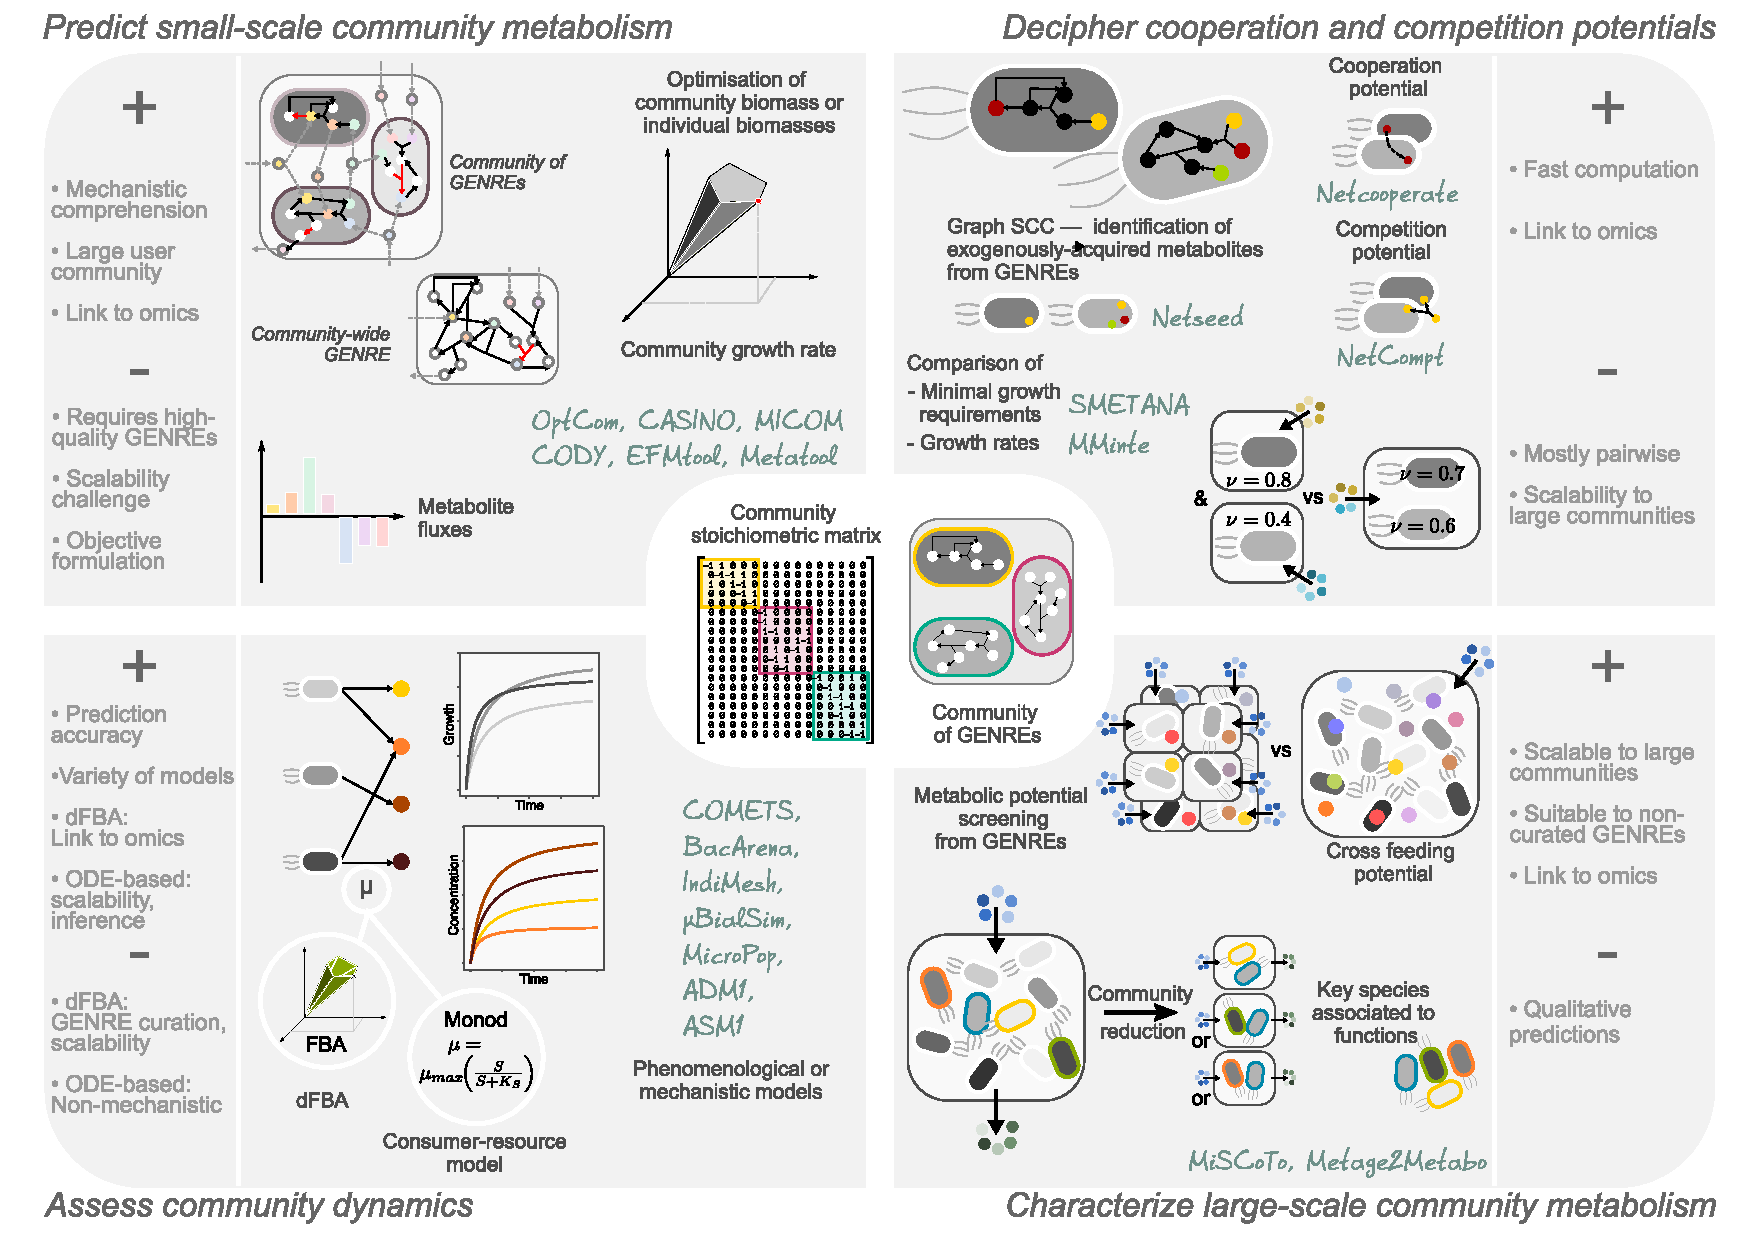
\includegraphics[width=\textwidth]{img/EDLA/review-methode.pdf}
    \caption{Liste non exhaustives des methodes qualitatives pour analyser une bactérie et des communautés avec leurs avantages et inconvéniants. Extrait de Cerk et al. \textit{Community-scale models of microbiomes: articulating metabolic modelling and metagenome sequencing}, 2023,Environmental Microbiology.[en révision]}
    \label{fig:my_label}
\end{figure}

\subsection{Défis rencontrés lors de l'analyse de la modélisation qualitative et quantitative du métabolisme des communautés}
Des questions similaires à celles déjà rencontrées (voir la sous section \ref{defi}) se posent également au niveau de la communauté. Les ensembles de métabolites produits en intracellulaire peuvent être disponibles pour l'ensemble des membres de la communauté. En effet, nous savons que les cellules sont capables de lyse cellulaire, libérant ainsi tous les produits métaboliques dans le milieu extra-cellulaire \citep{Fazzino2020}. De plus, les fuites métaboliques passives, c'est à dire sans coût énergétique pour la cellule, ont été montrées comme étant dominantes dans les interactions microbiennes  \citep{Pacheco.2019m3q}. Une seconde notion à prendre en compte est celle de la frontière des compartiments métaboliques propre à chaque espèce de la communauté. 


\section*{Conclusion}
Dans ce chapitre, nous avons proposé une revue de la littérature sur la thématique de la modélisation du métabolisme, en présentant dans un premier temps une définition et différentes représentations d'un réseau métabolique. Et dans un second temps, une collection de méthodes quantitatives et qualitatives d'analyse du métabolisme à l'échelle d'une cellule et d'un écosystème bactérien a été détaillé.\\
Parmi les approches de modélisation du métabolisme, nous avons vu que les modèles numériques sont pertinents d'une part, pour leurs capacités à intégrer des types de données omiques au moyen de contraintes linéaires ou d'optimisation, et d'autre part, pour la précision numérique qu'ils offrent. Cependant, cette aptitude rend délicate leur utilisation à des communautés plus complexes pour des raisons de coûts, calculatoire et du temps passé par le modélisateur ou de la modélisatrice, et de disponibilités de données. \\
De façon alternative, l'approche par raisonnement de l'étude du métabolisme dépasse ces limites en faisant une abstraction booléenne du métabolisme. De plus, nous avons vu que cette approche par raisonnement fournit une explicabilité aux modèles. En revanche, la précision apportée par ces modèles reste néanmoins qualitative. \textit{In fine}, il existe pas de méthode universelle permettant de répondre à notre objectif, et un compromis doit être fait. Dans le reste de ce manuscrit, nous essayerons de mieux comprendre les apports et les enjeux de chaque type de modélisation dans le but de créer une approche hybride répondant à notre problématique.\\
Nous verrons ainsi, dans le chapitre \ref{ccmc}, une application de cette approche de raisonnement sur un ensemble d'écosystèmes et comment l'explicabilité d'un modèle permet de définir un score de coopération et de compétition pour une communauté donnée. \\
L'intérêt d'obtenir des modèles explicables sera particulièrement exploité au cours du chapitre \ref{enrichissement} consistant à (i) sélectionner un ensemble de communauté potentiellement d'intérêt à partir d'une ensemble de contraintes, (ii) intégrer une temporalité. \\
Enfin, les données nécessaire pour réaliser ces travaux se sont uniquement basés sur des données génomiques. Dans le cas idéal, plusieurs types de données omiques permettent d'apporter des informations à différents échelles du métabolisme. Ainsi, nous verrons au cours du chapitre \ref{tango}, la plus value des données multi-omiques sur l'analyse du métabolisme d'une communauté contrôlé composée de trois bactéries et le degré de précision que l'on peut obtenir concernant les mécanismes intercellulaires.

\end{document} %
% \newpage
% 
%\subfile{chapitres/tango2.tex}
%% %  \ifdefined\FromMain %
%  \else % 
%  	\documentclass[../main.tex]{subfiles}
%  	\let\FromMain\undefined
%    	\begin{document}
%  \fi
%

\documentclass[../main.tex]{subfiles}
\begin{document}

\chapter{Modèle numérique du métabolisme bactérien au cours de la production d'un fromage}
\label{tango}
\minitoc
Soumis au journal Metabolic Engineering \footnote{\url{https://www.sciencedirect.com/journal/metabolic-engineering}}

Une listes des abréviations propre au métabolisme est disponible à la fin de ce chapitre section \ref{abbreviation-metabo}.

%\doublespacing %% For correction

\newpage

\section{Introduction}
Au sein de ce chapitre nous allons aborder la question de comment un modèle numérique, tel que nous l'avons défini, permet de répondre à plusieurs enjeux biologiques avec un critère d'explicabilité  satisfaisant. Ce modèle numérique s'inscrit dans un projet, appelé TANGO \citep{Cao2021} où les objectifs sont multiples. Différentes productions de fromage à pâte pressée non cuites de 2,5kg ont été réalisées en triplicat avec les mêmes bactéries lactiques et propionique mais en suivant des itinéraires légèrement modifiés. Ces changements ont permis de mettre en évidence expérimentalement l'impact de ces itinéraires sur l'arôme du fromage. Nous proposons dans ce chapitre, d'identifier, à l'aide d'un modèle numérique, les voies métaboliques conduisant à la production des composés d'arômes, les métabolites échangés entre les espèces dans l'itinéraire standard de fabrication. 
%Nous utiliserons pour cela, les valeurs expérimentales quantitatives, que sont la concentration des métabolites et des densités bactériennes est nécessaire. \\
%Ainsi, la construction d'un modèle numérique du métabolisme précis, fiable et explicable est nécessaire.  \\

À notre connaissance il existe des modèles numériques du métabolisme, garantissant la fiabilité des résultats ainsi que la précision, cependant, ces modèles sont souvent "boîtes noires" et ne permettent pas d'obtenir une explication mécanistique des résultats \citep{Popp2020, Zomorrodi}.  Ainsi, ces méthodes numériques fournissent des résultats de simulations mais ne permettent pas d'expliquer les voies métaboliques activées. De plus, Popp et al précisent également que ces résultats ne doivent pas engendrer une interprétation biologique détaillée étant donné l'inférence de paramètres génériques. Une conséquence de ces modèles est la difficulté à inférer des processus de régulation biologique trouvés dans la littérature ou encore, d'intégrer des données hétérogènes. Il existe des méthodes permettant l'intégration de données omiques ou cinétiques, mais séparément. Ainsi, les travaux de \citep{Jenior2020} permettent d'intégrer des données méta-transcriptomiques au sein de modèles métaboliques à l'échelle du génome (GEM). Au moyen de ces données et d'une analyse parcimonieuse de la distribution des flux dans un réseau métabolique, ils identifient le chemin le plus coûteux représentant l'investissement d'une cellule dans la transcription. Avec les données de croissance cinétique, du pH ou encore de la métabolomique \citep{Ozcan.2020} ont construit un modèle dynamique afin de prédire des concentrations de métabolites et ont inféré des mécanismes biologiques appris à partir des données. Ayant à disposition des données hétérogènes similaires à \citep{Ozcan.2020}, nous avons développé une approche numérique prenant en compte l'hétérogénéité des données disponibles et garantissant une explicabilité des résultats obtenus.\\

En s'inspirant de la stratégie développée par \citep{Ozcan.2020}, optimisant les modèles individuels et de communautés avec les données, nous avons alors développé une stratégie itérative explicative permettant d'intégrer un ensemble de données: génomique de chaque souche, métabolomique, pH, croissance de bactéries, et des dosages de métabolites. Cette stratégie a consisté à extrapoler les modèles individuels optimisés à partir des données et de la littérature pour prédire les comportements en communauté de chaque souche bactérienne, les concentrations de métabolites bactériens produits pendant la fermentation, la biomasse, ainsi que les interactions basées sur l'échange de métabolites bactériens entre espèces. Notre modèle numérique repose sur l'étude du métabolisme de trois souches bactériennes, que sont \textit{Propionibacterium freudenreichii} CIRM-BIA122, \textit{Lactiplantibacillus plantarum} CIRMB-BIA465 et \textit{Lactococcus lactis} biovar \textit{diacetyl lactis} CIRM-BIA1206. Tout d'abord, nous avons reconstruit le métabolisme de chaque souche microbienne en utilisant les données génomiques, puis, procédé au raffinement manuel des réseaux métaboliques au moyen de la littérature et des données de dosage. Dans un second temps, une étape de calibration dynamique utilisant les données de dosages, de pH, de croissance et la littérature a permis de garantir la précision et de la fiabilité de chaque modèle individuel. \\

Les travaux présentés dans ce chapitre ont mené à la soumission d'un article \footnote{\url{https://www.biorxiv.org/content/10.1101/2023.05.05.539417v1}} de journal \citep{Lecomte2023} en cours de publication et de plusieurs présentations scientifiques et posters \maxime{lien vers HAL}.


\section{Méthode pour la construction d'un modèle numérique du métabolisme}
Afin de construire un modèle numérique du métabolisme, les réseaux métaboliques à l'échelle du génome doivent être reconstruits à partir d'un génome annoté, curés et idéalement calibrés avec ces données multi-omiques. Nous décrirons dans un premier temps l'ensemble des données nécessaires, puis l'étape de reconstruction d'ébauche de réseaux métaboliques. Dans un second temps, nous verrons en détails l'approche itérative développée au moyen de l'étape de curation et de calibration dynamique des modèles.

\subsection{Présentation des données}

\subsubsection{Données omiques}

\paragraph*{Génomique}
Les souches utilisées sont décrites dans \citep{Cao2021}. Brièvement, la communauté bactérienne contrôlée est composée de deux bactéries lactiques (LAB), \lactis subsp. \textit{lactis} biovar \textit{diacetylactis} CIRMBIA1206 (nommée \lactis), \plantarum CIRMBIA465 (nommée \plantarum), et une bactérie propionique \freud CIRMBIA122 (nommée \freud) provenant du Centre International de Ressources Microbiennes des Bactéries d'Intérêt Alimentaire (CIRM-BIA\footnote{\href{https://collection-cirmbia.fr/}{https://collection-cirmbia.fr/}}). Leur génome a été séquencé, assemblé et a été intégré sur la plateforme MicroScope hébergée au Genoscope (CEA, Évry, France) pour une annotation automatique selon \citep{Vallenet.2019}. Les génomes annotés sont disponibles à l'ENA (EBI, Cambridge) sous le numéro d'accession PRJEB54980.


\paragraph*{Métatranscriptomique}
Un protocole détaillé est décrit dans les travaux de \citep{Cao2021}, nous décrivons ici que les étapes principales. Les données métatranscriptomiques ont été obtenues à cinq étapes de la fabrication du fromage: moulage, démoulage, après saumurage et affinage à 4 et 7 semaines. Les lectures sont disponibles à l'ENA (EBI, Cambridge) sous le numéro d'accession PRJEB42478. Ces lectures ont été alignées sur un génome de référence afin de déduire des informations relative à l'expression des gènes, puis uneétape de comptage à lieu. Les données brutes de comptage de RNASeq ont été normalisées en deux étapes. Tout d'abord, un facteur d'échelle spécifique à l'espèce a été appliqué pour éliminer les biais de composition entre les différentes bibliothèques utilisées en utilisant la méthode TMM (Trimmed Mean of M- Values) telle qu'implémentée dans le package edgeR version 3.32.1 \citep{Robinson2010}. Une étape supplémentaire de normalisation (du type RPKM) au sein de l'échantillon a été réalisée pour corriger la longueur des gènes et permettre la comparaison. Enfin, la moyenne des réplicats a été calculée.
%Pour chacune des trois espèces, elles ont été calculées en utilisant tous les gènes de l'espèce considérée et deux autres rangées pour l'autre espèce, calculées comme la somme des comptages attribués à chacune de ces deux autres espèces, 

\paragraph*{Métabolomique}
Les méthodes sont décrites dans \citep{Cao2021}. Brièvement, les sucres et les acides organiques dans les échantillons ont été quantifiés en utilisant la chromatographie liquide à haute performance (HPLC). Les composés volatils ont été analysés en utilisant l'extraction par sorption de l'espace de la tête (HS) et couplés à la chromatographie en phase gazeuse-spectrométrie de masse (GC-MS).

\subsubsection{Données de calibration}
\label{données-calibration}

Un suivi cinétique de la croissance bactérienne et du pH a été réalisé sur lait pour chaque souche individuelle. De plus, les concentrations en acides organiques pour \freud ont été évaluées en condition microaérophile (Table \ref{table:pure-culture-data}). Le milieu de culture de \freud a été supplémenté en lactate pour reproduire la croissance en co-culture et en hydrolysat de protéine du lait simulant sa protéolyse. En prenant en compte toutes ces conditions, chacune des souches a atteint un seuil de cultivabilité supérieure à 8 $\text{log}_{10}$ CFU/g. Le pH, d'une valeur de 6.7 lors de l'inoculation des deux bactéries lactiques, a atteint respectivement 5.7 et 5.1 pour \plantarum et \lactis. Pour \freud, \plantarum et \lactis, le début de la phase plateau, correspondant à l'entrée en phase stationnaire, a mis respectivement 48, 14 et 8 heures. Les données de dosage des métabolites de \freud montrent une production de propionate élevée (8 grammes par litre de lait), une forte consommation de lactate (9 grammes par litre de lait) et une faible production d'acétate et de succinate, respectivement 3,07 grammes par litre de lait et 0,371 gramme par litre de lait \ref{table:acids-dosage}). 

\paragraph*{Données cinétique de croissance et de pH}
Pour chaque souche nous avons collecté les données de croissance et de pH qui ont servi à calibrer dynamiquement notre modèle. Elles sont représentées dans la table \ref{table:pure-culture-data}.

\begin{table}[H]
\centering
\begin{adjustbox}{width=0.6\textwidth}
\begin{tabular}{|c|c|c|c|}
\hline
GEM & Temps & Densité bactériennes & pH  \\
 \hline
 \TableBac{\freud}{7} 
 & & & \\
 &  0 & 0.000001 & ø \\
 & 23 & 0.000099 & ø \\
 & 40 & 0.000561 & ø\\
  & 48 & 0.000412 & ø\\
  & 130 & 0.000710 & ø\\
  & & & \\
 \hline
 \TableBac{\plantarum}{7} 
  & 0 & 1.485e-06 & 6.7\\
  & 5 & 3.795e-06 & 6.68\\
  & 7 & 5.28e-06 & 6.66\\
  & 9 & 8.415e-06 & 6.555\\
  & 14 & 1.386e-05 & 6.54\\
  & 16 & 2.3595e-05 & 6.51\\
  & 79 & 3.762e-05 & 5.705\\
 \hline
 \TableBac{\lactis}{7} 
  & 0  & 8.25e-07 & 6.7\\
  & 5 & 5.230500e-05 & 6.49\\
  & 7 &6.831e-05 & 6.315\\
  & 9 & 6.649500e-05 & 6.075\\
  & 14 & 6.468e-05& 5.935\\
  & 16 & 4.735e-05 & 5.865 \\
  & 79 & 6.171e-05 &5.115\\
\hline
\end{tabular}
\end{adjustbox}
\caption{\textbf{Données de cultures pures utilisés pour calibrer chaque souche. Temps en heures et les valeurs de densités bactériennes représentent des moyennes sur les différents réplicats en 
$\text{g.DW}^{-1}$.} \label{table:pure-culture-data}}
\end{table}



\paragraph*{Les données de dosage d'acide}
Les dosages des acides lactiques, de l'acétate, du succinate et du propionate lors de l'inoculation de la souche et en fin de fermentation de \freud sont représentées dans la table \ref{table:acids-dosage}.

\begin{table}[H]
\centering
\begin{adjustbox}{width=1\textwidth}
\begin{tabular}{|c|c|c|c|}
\hline
Acides & Concentration $T_0$ & Concentration $T_{f}$ = 89 h  & Erreur standard \\
\hline
Lactate & 16.5 & 7.88 & 0.08 \\
Acetate & 0 & 3.07 & 0.02\\
Succinate & 0 & 0.371 & 0.063 \\
Propionate & 0 & 8.31 & 0.02 \\
 \hline
\end{tabular}
\end{adjustbox}
\caption{\textbf{Données de dosage d'acide en g/L pour \freud.}}
\label{table:acids-dosage}
\end{table}

\paragraph*{Données de croissance et de pH en communauté}
\label{com_data}
Au regard de notre stratégie itérative, les données représentées par la table \ref{table:co-culture-data} ont servi de données tests pour évaluer la précision du modèle. Toutes ces données proviennent de l'article de \citep{Cao2021}. Un suivi de la croissance des bactéries ainsi que de la production des métabolites ont été réalisés durant la fabrication du fromage. Les seuils de cultivabilité de \lactis, \plantarum et \freud ont atteint respectivement 8.45 $\log_{10}$CFU/g, 8.47 $\log_{10}$CFU/g et 8.59 $\log_{10}$CFU/g en approximativement 1200 heures.

\begin{table}[H]
\centering
\begin{tabular}{|c|c|c|c|c|}
\hline
GEM & Etapes & Temps (h) & \begin{minipage}[t]{0.4\linewidth}Population bactérienne (log$_{10}$ CFU/g) \end{minipage} \\
 \hline
 \TableBac{\freud}{6} & Linoc & 0 & 6.1 \\
 & Finoc & 18 & 6.1 \\
 & Cm & 19.5 & 7.16 \\
  & C0w & 60 & 8.11 \\
  & C4w & 732 & 8.56 \\
  & C7w & 1236 & 8.59 \\
  & & & \\
 \hline
 \TableBac{\plantarum}{6} & Linoc & 0& 5.2\\
  & Finoc &18 & 5.4 \\
  & Cm &19.5& 6.49 \\
  & C0w &60& 7.92 \\
  & C4w &732& 8.47 \\
  & C7w &1236& 8.47\\
 \hline
 \TableBac{\lactis}{6} & Linoc &0& 5.7 \\
  & Finoc &18& 7.5\\
  & Cm &19.5& 8.78\\
  & C0w &60& 9.06\\
  & C4w &732& 8.95 \\
  & C7w &1236& 8.45\\
\hline
\end{tabular}
\caption{\textbf{Donnes de croissance en co-culture pour tester les prédictions de notre modèle de communauté} \label{table:co-culture-data}}
\end{table}


\begin{table}[H]
\centering
\begin{tabular}{|c|c|}
\hline
Etapes & pH \\
\hline
Finoc & 6.717  \\
Cm &  6.362\\
C0w&  5.35 \\
C4w& 5.165  \\
C7w& 5.189 \\
 \hline
\end{tabular}
\caption{\textbf{Données de pH.}}
\label{table:ph-coculture}
%\caption{Données de communauté utilisé pour tester les prédictions à l'échelle de la communauté.}
\end{table}

\paragraph*{Conversion des unités}
Lors de la calibration, nous avons appliqué un coefficient multiplicateur de $0.33\times10^{-12}$ transformant les CFU en gramme de matière sèche. En effet, d'après \citep{Bakken1983}, $1\text{cm}^3$ de bactéries équivaut à 0.33 de matière sèche de biomasse et en supposant que 1 CFU a pour volume $1 \mu\text{m}^3$, nous avons donc : $1 \text{CFU} = 10^{-12} \text{cm}^3 \text{ soit } 0.33 \times10^{-12} \text{g.DW}^{-1}$. Nous avons dû également convertir les unités des métabolites que l'on suit en dynamique, de g/kg de lait en mmol/g de lait.



\subsection{Du génome annoté au réseau métabolique à l'échelle du génome}
Pour construire un modèle numérique du métabolisme de la production du fromage, nous avons reconstruit les réseaux métaboliques à l'échelle du génome avec l'outil de reconstruction CarveMe \citep{Machado2018} version 1.4.1 et enrichi l'annotation existante avec ModelPolisher \citep{Romer2016} version 2.0 en ajoutant des métadonnées liées aux identifiants BIGG depuis la base de connaissance BIGG \citep{King2016}. Afin de vérifier la qualité des GEM, chaque modèle métabolique a été validé avec MEMOTE \citep{Lieven.2020} version 0.13.0.

\subsection{Modélisation et implémentation numérique}

\subsubsection*{Analyse statique}
Pour permettre une analyse numérique des réseaux métaboliques, nous avons développé notre stratégie numérique itérative en se basant sur l'analyse par équilibre des flux (FBA)\citep{Orth2010}. Brièvement, à partir de la composition nutritionnelle du lait, le FBA calcule une distribution de flux optimale satisfaisant la st\oe{}chiométrie des contraintes thermodynamiques et maximisant une fonction objective, ici la réaction de biomasse.

\begin{equation}
\label{eq:fba}
\text{trouver }v^* \in \R^{N_r} \text{ tel que }  v^*= \argmax_{\begin{array}{c} S.v=0 \\ v_{min}^{in} \leq v \leq v_{max}^{in} \\ v_{min}^{ex} \leq v \leq v_{max}^{ex}   \end{array}}   v_{biomasse}
\end{equation}
ou $v_{biomasse}$ est le flux de la réaction de biomasse de modèle, $S$ est la matrice st\oe{}chiométrique dérivée du modèle métabolique, $v_{min}^{in}$ et $v_{max}^{in}$ (resp. $v_{min}^{ex}$ et $v_{max}^{ex}$) définissant les bornes de flux intracellulaires ou d'échanges pour le vecteur de flux $v$ contenant $\R^{N_r}$dimension. 

L'équation \eqref{eq:fba} définit alors, pour chaque bactérie $i$, la correspondance $\mu_{i}$ entre les vecteurs de contraintes sur les réactions d'échange définissant l'environnement nutritionnel et le flux optimal $v^*$ obtenu dans ce contexte nutritionnel.
\begin{equation}
\mu_{i}(v_{min}^{ex},v_{max}^{ex}) = v^*
\label{eq:mu-fba}
\end{equation}

Dans un souci de garantir une solution unique, l'ordre lexicographique \citep{gomez2014dfbalab} a été utilisé, c'est à dire, nous avons défini la direction du flux d'échange des métabolites suivis dynamiquement, définissant de nouvelles contraintes à satisfaire et réduisant l'espace de solution.

\subsubsection*{Analyse dynamique}
\label{dynamic analyse}

Ayant à notre disposition les données cinétiques de chaque souche individuelle ainsi qu'en communauté, nous avons implémenté le dynamisme de cette communauté bactérienne en s'inspirant de l'analyse par équilibre des flux dynamique (dFBA) de \citep{Mahadevan2002} et en ajoutant ainsi des mécanismes dynamiques de population au modèle FBA.\\

Le premier mécanisme que l'on a décrit dynamiquement est le \textit{quorum sensing}, correspondant au processus de régulation de la population sur la croissance de la population. Notons $b=(b_i)$ pour $i \in \mathcal{B}=\{\lactis,\plantarum,\freud\}$ les densités de la population bactérienne et $\mathcal{R}_{i}$ le vecteur modélisant ce processus, le \textit{quorum sensing} a été modélisé de la façon suivante:

\begin{equation}
\label{eq:logistic-growth}
    \mathcal{R}_{i} = \lambda_i (1-\frac{b_i}{\beta_i}), \text{ for }i \in \mathcal{B} 
\end{equation}

où $\lambda_i$ est un poids et $\beta_i$ est la capacité de charge de la population, correspondant à la valeur de la phase plateau de chaque bactérie dans l'expérience.


Nous avons par la suite défini des flux d'import de composés présents dans le modèle. Pour un substrat $j$, un modèle métabolique $i$ et $m=(m_j)_{1\leq j \leq N_m}$ la concentration $m$ de composés métaboliques $N_m$ qui sont expérimentalement suivis, le flux de la borne inférieure $c^{ex}_{min,i,j}$ et supérieure $c^{ex}_{min,i,j}$  ont été définis comme suit:

\begin{equation} 
c^{ex}_{min,i,j} = max(-\frac{m_j}{\Delta t \sum_{i\in \mathcal{M}_j} b_i},v^{int}_{i,j}) \quad \quad c^{ex}_{max,i,j} = 0,
\label{eq:usual-consumption-limitation}
\end{equation}

où $\mathcal{M}_j$ est le sous-ensemble de bactéries métabolisant $j$ et $\Delta t$ est un l'intervalle temporel d'importation. Ces équations reflètent le partage uniforme des ressources parmi les bactéries durant la fenêtre temporelle $\Delta t$. Quand les substrats sont en excès, le flux est limité par la limite d'import intrinsèque $v^{int}_{i,j}$, il est partagé équitablement entre les bactéries le consommant $-\frac{m_j}{\Delta t \sum_{i\in \mathcal{M}_j} b_i}$.

Nous avons par la suite modulé le flux des bornes inférieures $c^{ex}_{min,i,j}$ des composés que l'on suit en dynamique correspondant aux composés des données biochimiques. En s'inspirant de l'approche de \citep{Ozcan.2020}, nous avons régulé le métabolisme du lactose chez les bactéries lactiques. Elle est ainsi modulée négativement par la forme non dissociée de l'acide lactique avec une décroissance exponentielle. Pour $j=lcts\_e$ et $i \in \{\lactis, \plantarum\}$, les flux des bornes inférieures $c^{ex}_{min,i,j}$ sont définis par: 

\[ c^{ex}_{min,i,j} = max(-\frac{m_{lcts_e}}{\Delta t*\sum_{i \in \mathcal{M}(lcts_e)} b_i},-\mu_{max,lcts}*10^{(-k_{lac}*\phi_{undiss})}-\mu_{min,lcts})\]  


où $k_{lac}$ correspond à la décroissance exponentielle, $\mu_{max,lcts}$ et $\mu_{min,lcts}$ sont les valeurs maximales et minimales et $\phi_{undiss}$ est une fonction calculant la concentration de la forme non dissociée de l'acide lactique à partir du lactate. Cette fonction $\phi_{undiss}$ est dérivée de l'équation de Henserson-Hasselbalch comme dans \citep{Ozcan.2020} et s'écrit 
\begin{equation}
\phi_{undiss}(m_{lac\_\_L\_e},m_{lac\_\_D\_e}) = \frac{m_{lac\_\_L\_e}+m_{lac\_\_D\_e}}{1+ 10^{c_1 * (m_{lac\_\_L\_e}+m_{lac\_\_D\_e})+c_2}}.
\label{eq:undissociated-lactate}
\end{equation}

Dans cette équation, le terme $c_1 * (m_{lac\_\_L\_e}+m_{lac\_\_D\_e})+c_2$ est une approximation linéaire de $(pH-pKa)$, alors que les paramètres 
$c_1$ et $c_2$ sont inférés par une régression linéaire des données de co-cultures. La production de lactate est régulée de la même manière, alors que la production d'acétate est régulée en fonction de la disponibilité en lactose. 
%Voir matériel supplémentaire section \ref{sec:dynamics-bounds} pour une description détaillée et justifications des bornes dynamiques configurées sur les réactions d'échange.

Pour \freud, les bornes supérieures de production sont calculées à partir des dosages de métabolites et des données de croissance dans les expériences de culture pure, en supposant un flux constant.\\

%(voir le matériel supplémentaire \ref{sec:estimate-bounds-freud}).
Pour $i\in \mathcal{B}$ et $1\leq j \leq N_m$, nous avons donc le système final suivant décrivant la densité de bactérie $\partial_t b_i$ et la concentration de métabolites $\partial_t m_j$ au cours du temps:

\begin{align}
    \label{eq:system_dynamics_b}
    \partial_t b_i& = \mathcal{R}_{i}(b_i) {\mu}_{i,i}\left((c^{ex}_{min,i},c^{ex}_{max,i})(b,m)\right) b_i  \\
    \label{eq:system_dynamics_m}
    \partial_t m_j &= \sum_{i \in \mathcal{B}} {\mu}_{i,j}\left((c^{ex}_{min,i},c^{ex}_{max,i})(b,m)\right) b_i 
\end{align}
dans lequel le terme ${\mu}_{i,i}$ est la composante correspondant au métabolite $j$ (ou à la biomasse $i$) de $\mu_i$, calculé à partir de \ref{eq:mu-fba} compte tenu de l'ensemble des contraintes $(c^{ex}_{min,i},c^{ex}_{max,i})(b,m)$. Ces contraintes dépendent dynamiquement de l'état de la variable $b$ et $m$, c'est à dire, de la densité de $b$ au cours du temps ($\partial_t b_i$) et de la quantité de $m$ disponible calculée par $\partial_t m_i$. 





\subsubsection*{Implémentation numérique} 
Le système dynamique est résolu avec le schéma semi-implicite d'Euler. A chaque étape $n$, après le calcul de $F_j$ correspondant au flux total du composé $j$ comme défini par l'ensemble des GEMs, 

\[ F_j=\sum_{i \in \mathcal{B}} {\mu}_{i,j}\left((c^{ex}_{min,i},c^{ex}_{max,i})(b^n,m^n)\right) b_i \,,\]

nous calculons les densités bactériennes ($b_i^{n+1}$) et la concentration du composé $j$ ($m_j^{n+1}$) au temps suivant:

\begin{align*}
b_i^{n+1}& = b_i^n+\Delta t* F_{b_i} \\
m_j^{n+1}& = \begin{cases} m_i^n+\Delta t* F_{j} & \text{ si } F_j>0 \text{(cas explicit)}\\
m_j^n/(1-\Delta t * F_j/m_j^n) & \text{ sinon (cas implicite)}
\end{cases}
\end{align*}

Ce schéma semi-implicite d'Euler a été utilisé pour garantir la positivité de la solution. En effet, en n'utilisant uniquement le cas explicite lorsque $F_j$ est négatif, la densité de la bactérie $b_i^{n+1}$ le sera également. Le cas implicite seul serait une solution mais augmenterait le temps de calcul. Nous avons établi un compromis en développant ce schéma semi-explicite.

\subsection{Raffinement des modèles métaboliques individuels}
Pour retrouver les comportements observés dans la littérature, les réactions à ajouter ou à contraindre dans les GEMs diffèrent, mais le processus itératif de vérification reste le même. Au moyen d'une analyse par équilibre des flux (FBA) \citep{Orth2010} maximisant la biomasse de chaque souche, les voies métaboliques activées, c'est à dire celles pour lesquelles un flux non nul est présent, peuvent être détectées. La première étape consiste à vérifier si toutes les voies métaboliques d'intérêt sont fonctionnelles de manière qualitative, \textit{i.e.} observation de production, de consommation et activation ou non de voies métaboliques. Lors d'une inactivation \textit{in silico} dans le modèle de voies partielles de voies métaboliques, nous avons développé le protocole suivant: détection de fuite de flux symbolisée par des valeurs de flux extrêmes, identification d'activation de voies métaboliques incohérente avec l'état des connaissances de l'organisme, ajustement des valeurs de bornes de régulation ou blocage de réactions. Pour chaque modification apportée, une vérification de la distribution des flux est faite jusqu'à obtenir les observations souhaitées.

\subsection{Calibration des modèles métaboliques individuels}
Afin de retrouver numériquement les valeurs expérimentales de chaque souche, nous avons calibré chacun de nos modèles métaboliques. Pour rappel, notre stratégie a consisté à obtenir des modèles individuels suffisamment précis pour déduire des comportements mécanistiques à l'échelle de la communauté. Nous avons donc estimé des paramètres propres à chaque souche, modifiant les flux d'import des métabolites d'intérêt en résolvant le problème de minimisation $J$ suivant pour les bactéries lactiques (équations \eqref{eq:optim_LAB}) 

\begin{equation}
J(b_i,pH | \theta_i, b_{i,exp},pH_{exp} ) = \left \Vert \frac{\logten(b_i) - \logten(b_{i,exp})}{\sigma_{log,i,exp}} \right \Vert^2 + \alpha \left \Vert\frac{pH - pH_{exp}}{\sigma_{pH,exp}} \right \Vert^2 
\label{eq:optim_LAB}
\end{equation}

où $\sigma$ (resp. $\sigma_{log,i}$) est l'écart-type (resp. l'écart-type log transformé) des données correspondantes, et $\theta_i = (k_{lac},\mu_{max,lcts})$ si $i=\lactis$ et $\theta_i = (k_{lac},\mu_{max,lcts},\lambda_i)$ si $i=\plantarum$, $b_i$ correspond à la densité de la population bactérienne de $i$, pour $i \in\{\lactis,\plantarum\}$ et $\alpha$ un poids.\\

Concernant \freud, la fonction coût cherchant à minimiser l'écart aux données est représentée par l’équation \eqref{eq:optim_freud}: 

\begin{equation} 
J(b,m | \theta_i, b_{exp},m_{exp} ) = \left \Vert \frac{\logten(b) - \logten(b_{exp})}{\sigma_{log,b,exp}} \right \Vert ^2 + \alpha \left \Vert \frac{m - m_{exp}}{\sigma_{m,exp}} \right \Vert^2 
\label{eq:optim_freud}
\end{equation}

où $m_{exp}$ est le dosage final d'acétate, lactate, propionate et succinate, et $\theta_i = (\lambda_i)$. \\

Afin d'éviter la sur-prédiction, nous avons délibérément optimisé un petit nombre de paramètres $\theta$ pour chaque souche. L'ensemble des paramètres ainsi que leurs rôles sont décrits dans la table \ref{table:optimised-parameter}:


\begin{table}[H]
\centering
\begin{adjustbox}{width=1\textwidth}
\begin{tabular}{|c|c|c|}
\hline
GEM & Paramètres & Explication  \\
 \hline
 \freud & $\lambda_i$ & Modification des bornes d'import des nutriments suivi en dynamique \\
 \hline
 \plantarum &$k_{lac}$ & Paramètre de la régulation de la consommation du lactose en fonction de la concentration de lactate  \\
  & $\mu_{max,lcts}$& Paramètre de la régulation de la consommation du lactose en fonction de la concentration de lactate \\
  & $\lambda_i$ & Modification des bornes d'import des nutriments suivi en dynamique\\
 \hline
 \lactis & $k_{lac}$ & Paramètre de la régulation de la consommation du lactose en fonction de la concentration de lactate \\
  & $\mu_{max,lcts}$& Paramètre de la régulation de la consommation du lactose en fonction de la concentration de lactate\\

\hline
\end{tabular}
\end{adjustbox}
\caption{\textbf{Ensemble des paramètres optimisés pour chaque modèle individuel avec leur fonction.} \label{table:optimised-parameter}}
\end{table}

%Les problèmes dFBA \eqref{eq:system_dynamics_b}--\eqref{eq:system_dynamics_m} ainsi que les paramètres inférés sont résolu en créant un scipt Python et en utilisant les bibliothèques \texttt{numpy} v.1.19.5\citep{harris2020array}, \texttt{pandas} v.0.25.3 \citep{mckinney2010data}, and \texttt{scipy} v.1.5.3 \citep{mckinney-proc-scipy-2010}. Durant le dFBA, le FBA est résolu en utilisant l'ordre lexicographique défini \citep{Gomez2018}.

\section{Application de la méthode numérique sur 3 souches du fromage}
Nous avons testé notre méthodologie itérative de raffinement et de calibration sur les 3 souches bactériennes présentées plus haut. L'objectif de cette application est triple: d'une part, montrer qu'à partir de modèles métaboliques individuels nous pouvons prédire numériquement des interactions, des concentrations de métabolites et de densités bactériennes, et d'autre part, être suffisamment "boîte-blanche" pour fournir des hypothèses testables sur des voies activées pour la production d'arômes dans le milieu extra-cellulaire. Enfin, ce modèle numérique doit être capable d'intégrer les données hétérogènes décrites plus haut. Dans la suite de ce chapitre, nous allons dans un premier temps nous focaliser sur les résultats des processus itératifs de raffinement et de calibration de modèles individuels. Une explication minutieuse des modifications réactionnelles et une validation souche par souche seront présentées. Puis, nous montrerons comment les données hétérogènes nous ont permis de calibrer dynamiquement nos modèles. Dans un second temps, nous présenterons l'implémentation du modèle de communauté ainsi que son exploration sur le plan des croissances bactériennes, de la production des composés d'arômes suivie en dynamique ainsi que sur les potentielles interactions métaboliques. Enfin, nous explorerons les possibles interactions bactériennes du modèle avec des outils sans \textit{a priori}: MICOM, SMETANA et M2M.


\begin{figure}
    \centering
    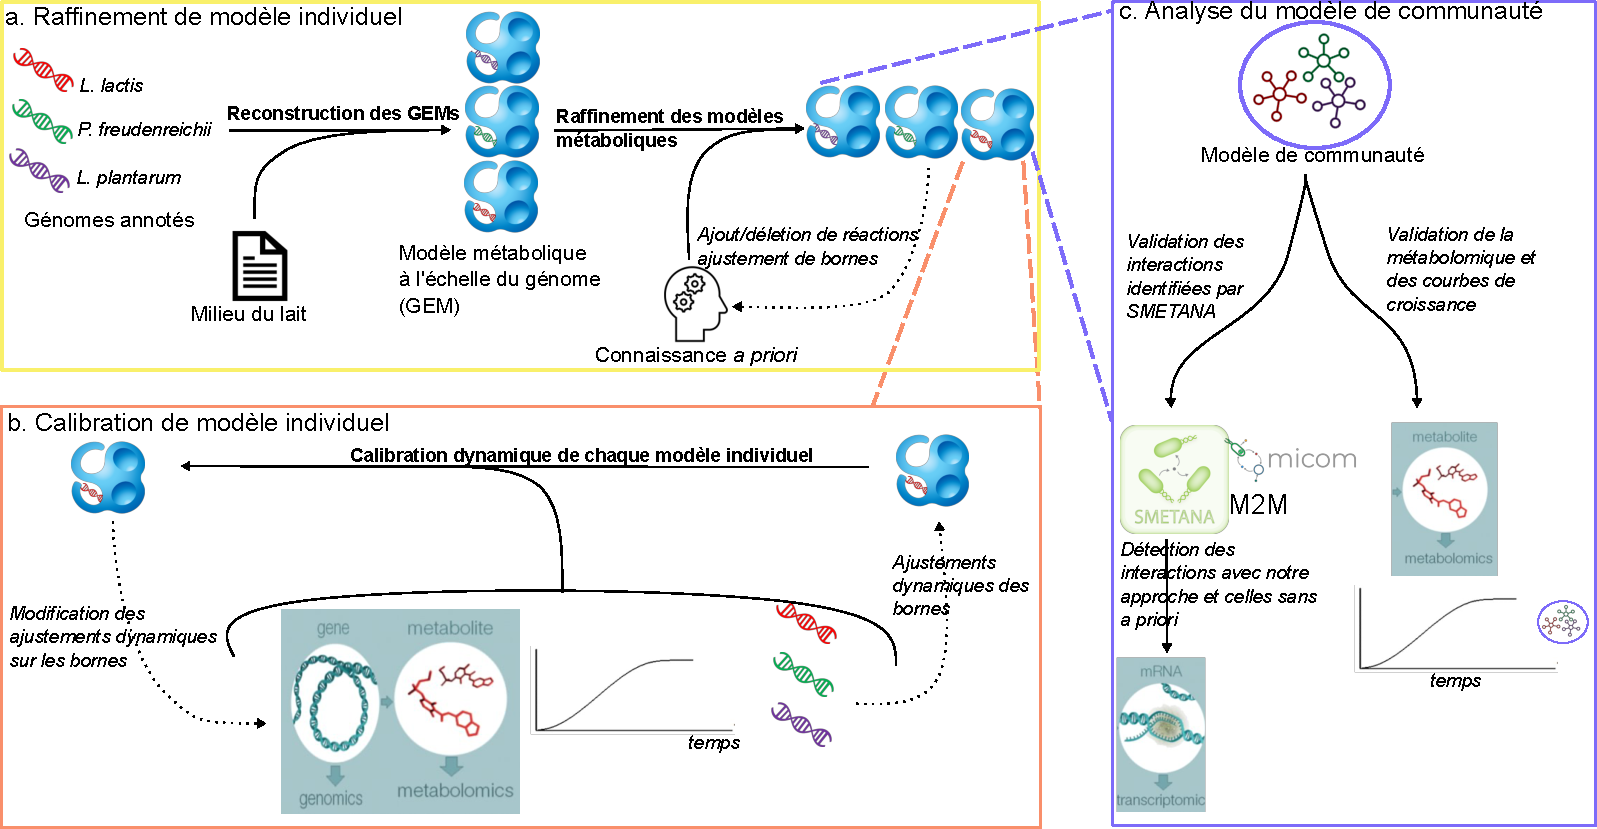
\includegraphics[width=\textwidth]{img/tango/global.pdf}
    \caption{Récapitulatif des étapes de raffinement et de calibration des modèles métaboliques, des simulations ainsi que des données utilisées}
    \label{fig:my_label}
\end{figure}

\subsection{A l'échelle de chaque souche}


\subsubsection*{Raffinement des modèles FBA individuels}
Les réseaux métaboliques à l'échelle du génome ont été reconstruits pour chaque souche individuelle depuis leurs séquences génomiques annotées respectives. Après une première étape automatique de reconstruction faite avec CarveMe, nous avons tout d'abord ajusté les flux des métabolites présents dans les réseaux métaboliques en cohérence avec la composition du lait. Les bornes inférieures de réactions d'échanges de composés qui n'apparaissent pas dans la composition du lait, sont ainsi mises à 0. La liste est constituée des réactions d'échange du glucose ($EX\_glc\_\_D\_e$) et du coenzyme A ($EX\_coa\_e$) pour \lactis et \plantarum, de l'amidon  ($EX\_starch1200\_e$) pour \lactis et \freud, du dihydroxyacetone  ($EX\_dha\_e$) pour \plantarum et \freud et du galactose ( $EX\_gal\_\_e$) pour \plantarum. \\


Nous avons ensuite réalisé un raffinement manuel du métabolisme carboné central basé sur la littérature et la connaissance biologique dans le but de prendre en compte les spécificités de chaque souche bactérienne. Le métabolisme carboné central produit du NADH and NADPH et ses formes réduites correspondantes, de l'ATP, et les précurseurs nécessaires pour la biosynthèse des molécules essentielles pour la croissance ainsi que pour l'activité métabolique des cellules bactériennes, e.g. acides aminés, purine, pyrimidine, glycerol-3-phosphate, acides gras, N-acetyl-glucosamine, vitamines. Parmi les voies métaboliques du métabolisme carboné central, la glycolyse et la voie des pentose phosphate sont communes aux trois espèces et presque identiques. Les sources de carbone telles que le lactose, l'acide citrique et l'acide lactique, sont converties en pyruvate, qui sera utilisé dans des voies spécifiques représentées dans les Figure \ref{figure:metabolic_map_freud},\ref{figure:metabolic_map_lactis},\ref{figure:metabolic_map_plantarum}. Dans la suite du chapitre, les caractéristiques métaboliques de chaque souche seront étudiées afin de justifier les raffinement faits, en se focalisant sur les voies métaboliques secondaires permettant la production de composés organoleptiques.


\paragraph*{Bactéries lactiques}
Les bactéries lactiques \lactis et \plantarum utilisent le lactose et le citrate, les deux principales sources de carbone du lait \citep{Widyastuti2014}. Le lactose est dégradé par l'enzyme beta-galactosidase en galactose et glucose, et ce dernier alimentent la glycolyse. Concernant le galactose et l'acide citrique, leur métabolisme dépend de la souche étudiée \citep{Palles1998}. D'un coté, le lactose est converti en glucose-6-phosphate \textit{via} la voie métabolique de Leloir avant d'entrer dans la glycolyse, et de l'autre l'acide citrique est converti en pyruvate par l'enzyme citrate lyase \citep{alma991000892589705596}. Du point de vue du métabolisme secondaire, le butanediol et le diacétyle sont responsables de la saveur beurrée du fromage, et sont produits par les deux modèles à partir du pyruvate grâce à la voie de l'acétolactate. L'ensemble des voies métaboliques décrites ci-dessus est récapitulé dans les Figures \ref{figure:metabolic_map_lactis} et \ref{figure:metabolic_map_plantarum}. \\



\subparagraph*{\lactis}
Pour permettre la production de certains composés d'intérêt, comme le butanediol, le GEM a été manuellement curé (Fig.~ \ref{figure:metabolic_map_lactis}). En reprenant la méthode de raffinement de modèle décrite plus haut, le flux de l'acétoine-dehydrogenase a été bloqué (ACTD2) permettant la production du butanediol. Les bornes de l'acétolactate decarboxylase (ACLDC) et de l'acétolactate synthase (ACLS) ont été modifiées de façon à permettre l'activation de la voie de l'acetolactate, comme retrouvé dans la littérature \citep*{Carroll1999,Swindell1996,Makhlouf2006}. Enfin, la consommation de lactose a été régulée en modifiant les bornes de la réaction LACZ ce qui a permis un flux de production de lactate pour \lactis (Fig.~ \ref{figure:metabolic_map_lactis}.

Pour valider ce modèle, nous avons considéré un exemple d'activation de voie métabolique durant la production du fromage, validable au regard de la littérature et des données de métatranscriptomiques. Il est montré que \lactis consomme le lactose à la fois par la voie du tagatose, codée dans l'opéron plasmidique \textit{lacABCD}, ou par la voie de Leloir, codée dans l'opéron du chromosome \textit{galKTE}. D'un point de vue des données metatranscriptomiques, \lactis exprime les gènes associés à la voie du tagatose au début de la production de fromage quand la concentration de lactose est grande, et ceux de la voie de Leloir durant l'affinage quand la concentration de lactose est faible. Cela suggère fortement que la concentration de lactose détermine quelle voie métabolique est employée, et prédit qu'une grande quantité de lactose dans le milieu nutritionnel devrait produire un flux important à travers la voie du tagatose. Le modèle FBA de \lactis est en accord avec les données métatranscriptomiques. Nous avons observé un flux important de dégradation du lactose à travers la voie du tagatose (Fig. \ref{dfba_metabolite_lactis}~a).

\begin{figure}[H]
    \centering
    % \hspace{-3.5cm}
    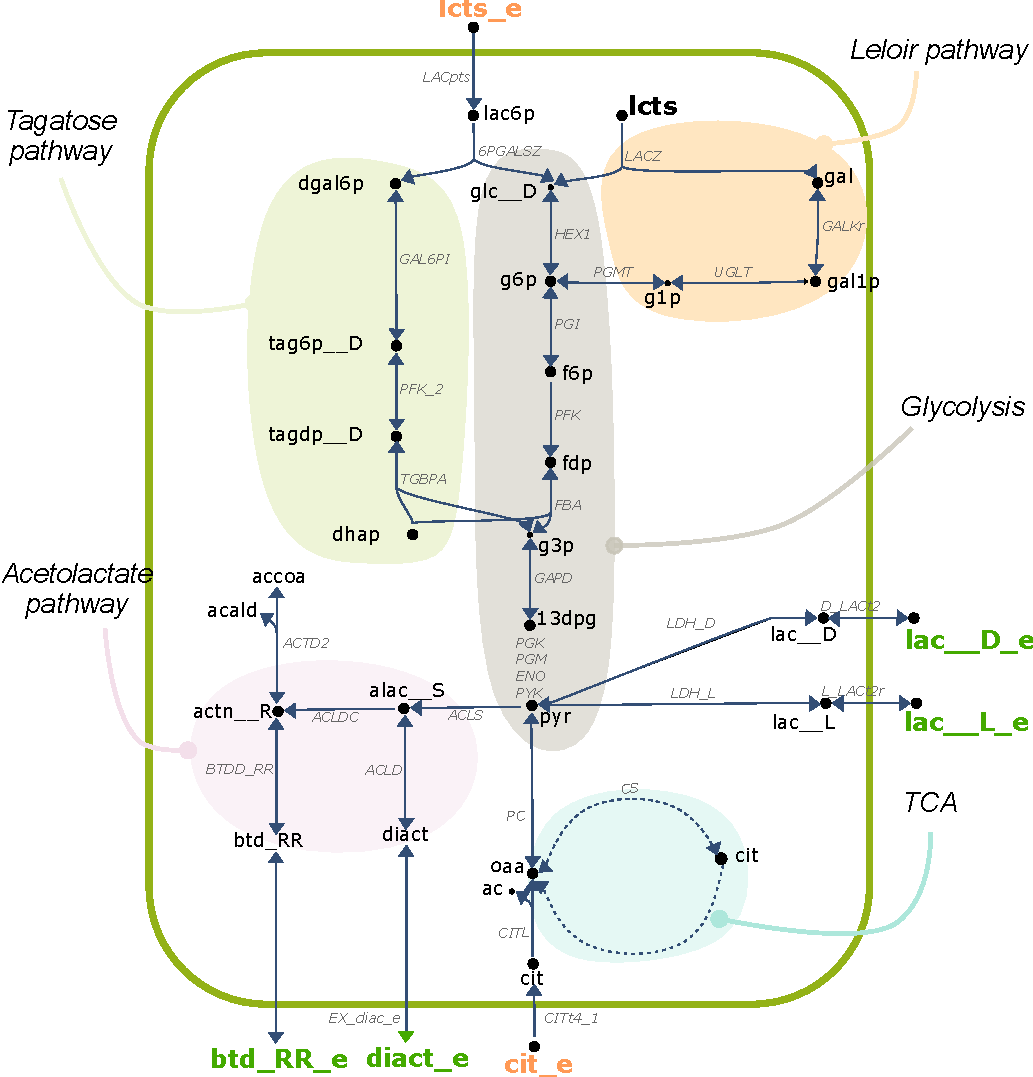
\includegraphics[width=1\textwidth]{img/tango/carte_lactis.pdf}
    \caption{\textbf{Cartes des voies métaboliques du métabolisme carboné central d'intérêt de \textit{L. lactis}}. La voie métabolique de la glycolyse est représentée en gris, celle de Leloir en saumon, acétolactate en rose, le cycle du TCA en bleu clair, et le tagatose en vert. Les métabolites en orange et vert correspondent aux entrées et sorties du modèle métabolique. La liste des métabolites et des réactions est répertoriée à la fin du chapitre à la section \ref{abbreviation-metabo} }
    \label{figure:metabolic_map_lactis}
\end{figure}

\subparagraph*{\plantarum}
L'exemple pris pour \plantarum concerne la dégradation du glucose et du galactose dans le cas des fermentations homolactique et hétérolactique (voir figure \ref{figure:metabolic_map_plantarum}. Dans les deux configurations, le pyruvate est produit à partir de la dégradation du glucose et du galactose. Durant la fermentation homolactique, le pyruvate est associé au relargage de l'acide lactique dans le milieu extracellulaire. Concernant la fermentation hétérolactique, on observe en plus une production d'éthanol et d'acétate. Nous savons que \plantarum est une bactérie hétérolactique pouvant produire de l'acétate grâce à l'enzyme transketolase (numéro EC 4.1.2.9) décrit dans \citep{Abedi2020} à travers la voie métabolique de l'acétate kinase. Pour permettre cette production dans notre modèle, nous avons bloqué la pyruvate formate lyase (PFL) \citep{Quatravaux2006}. Concernant le butanediol, la même curation que pour \lactis a été effectuée. Enfin, pour reproduire la dégradation du galactose et du glucose par la voie de Leloir et de la dégradation du lactose grâce à la $\beta$-galactosidase \textit{LACZ}, la réaction \textit{LCTSt3ipp} a été bloquée et la réaction UTP-glucose-1-phosphate uridylytransferase (\textit{GALUi}) a été rendue réversible pour compléter la voie de dégradation du galactose (Fig. \ref{dfba_metabolite_plant}~a).


\begin{figure}[H]
    \centering
    % \hspace{-3.5cm}
    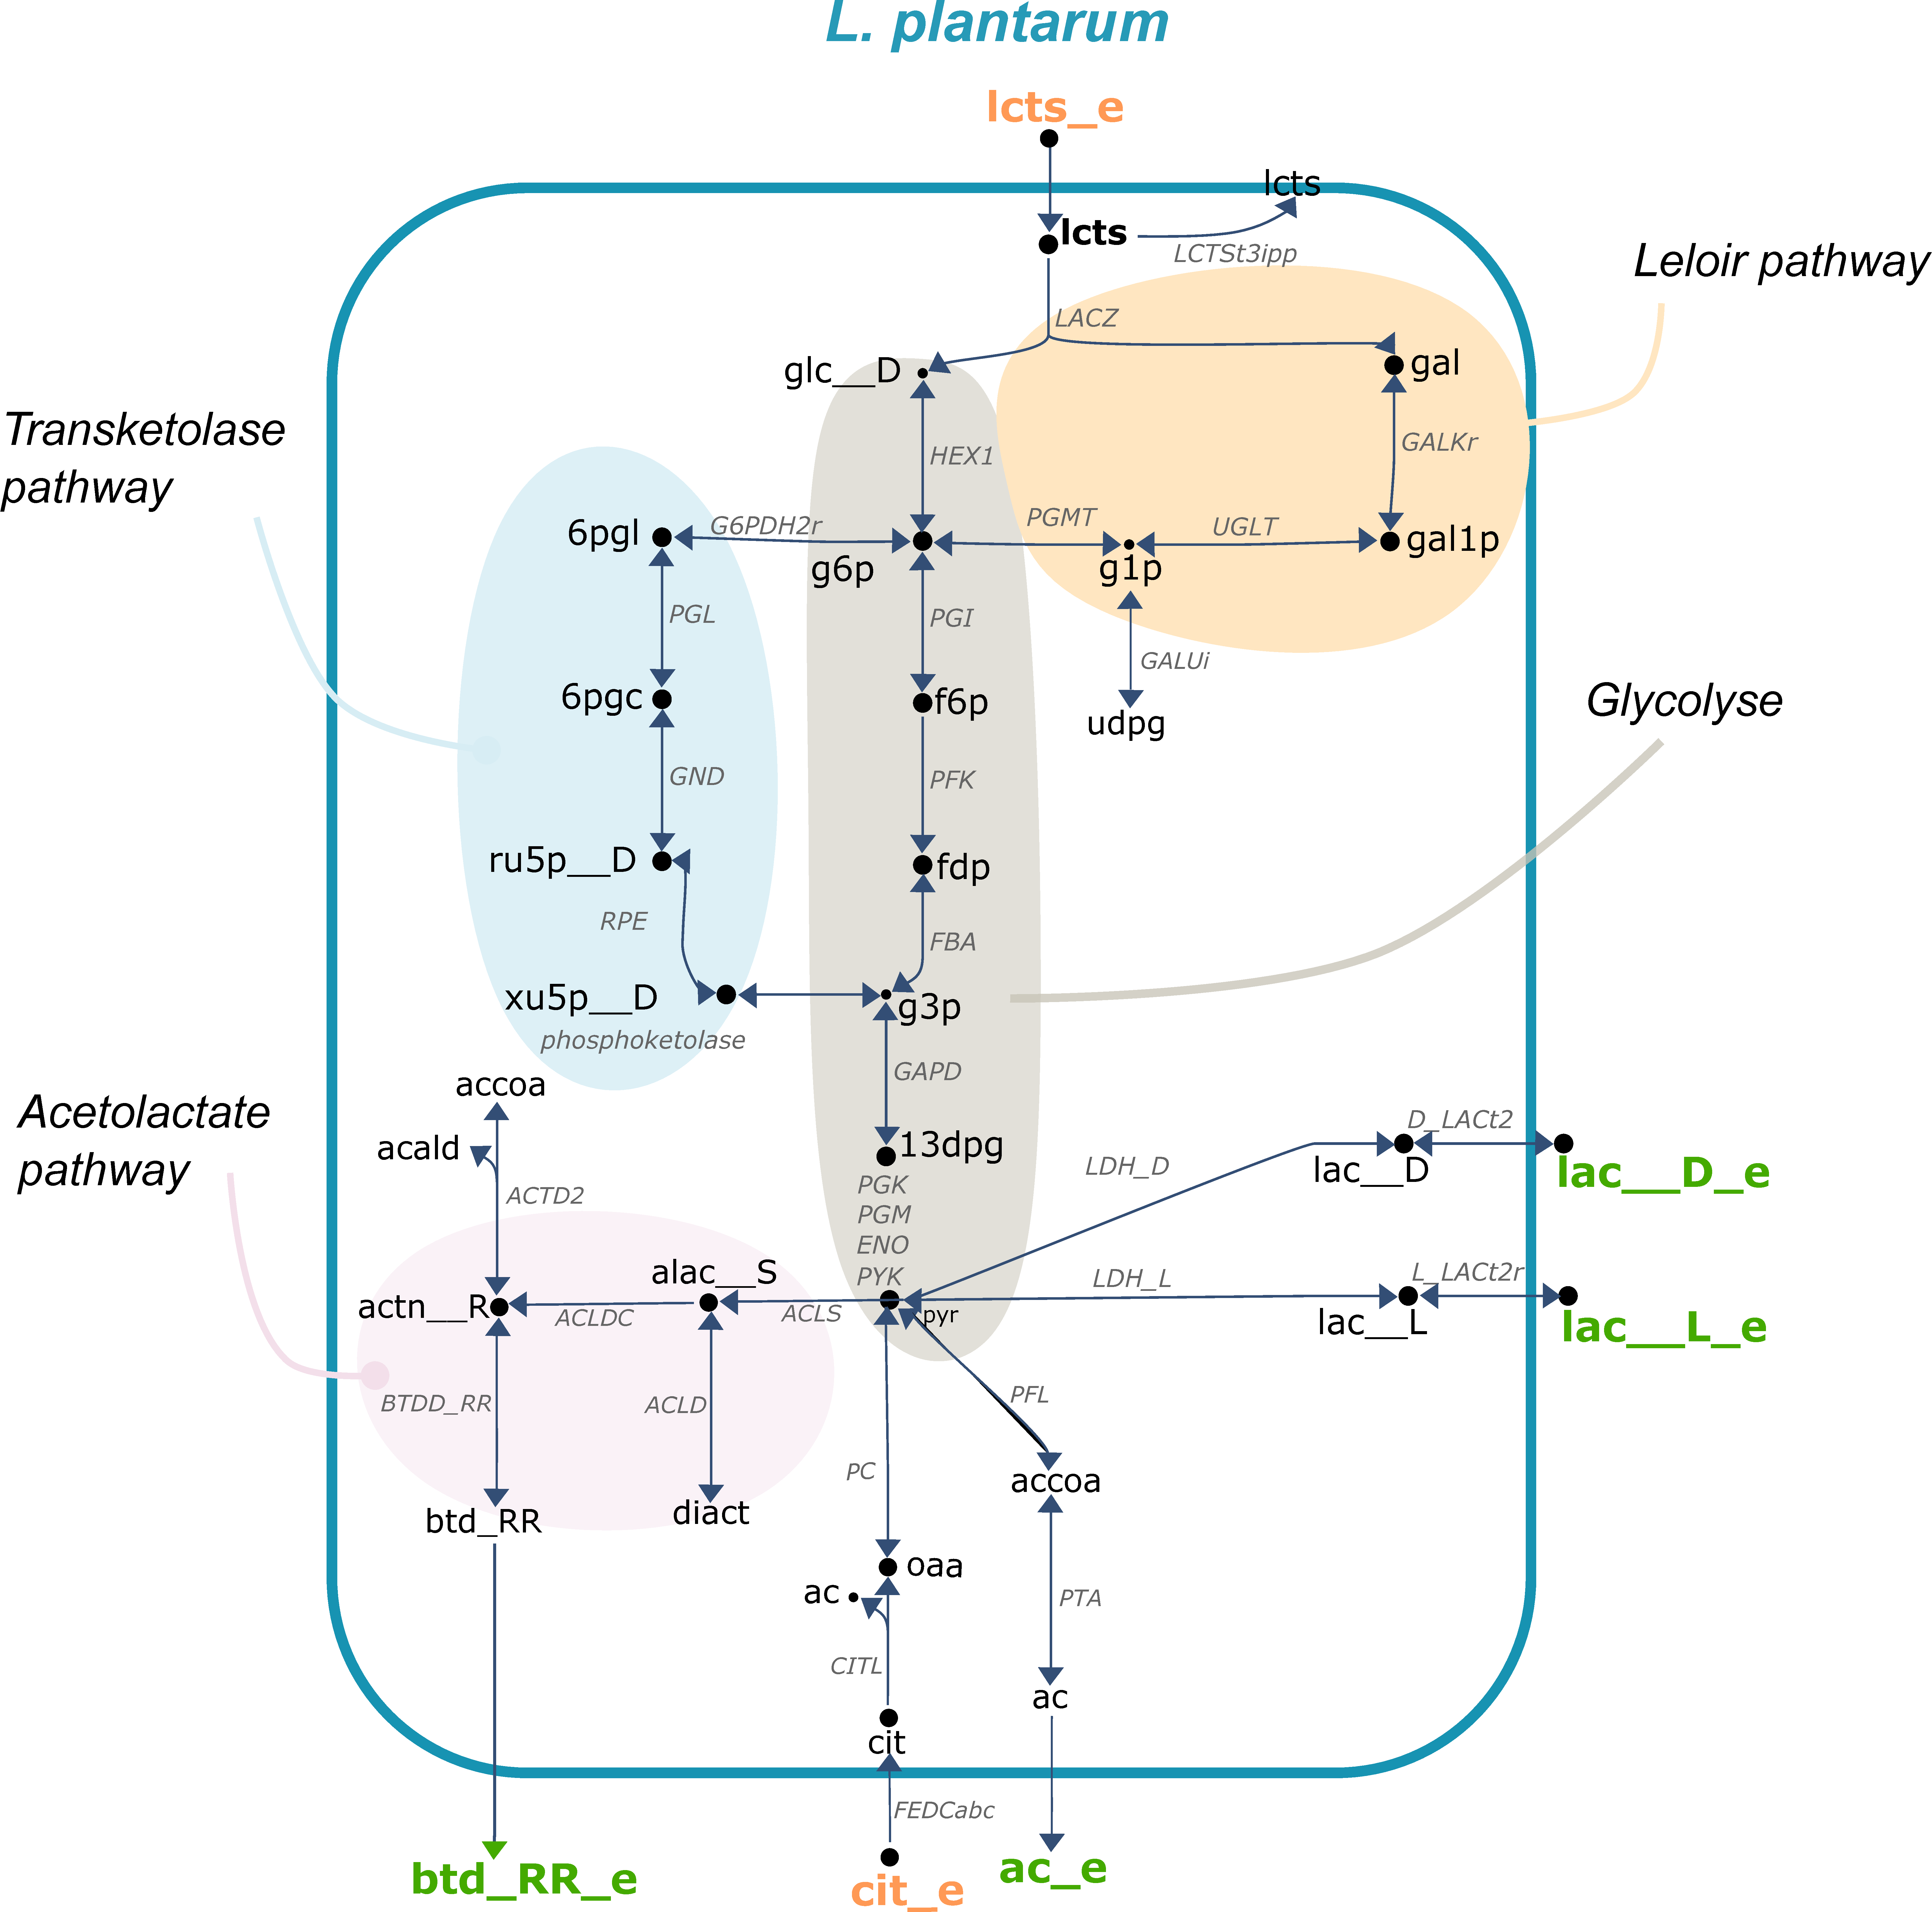
\includegraphics[width=1\textwidth]{img/tango/carte_plantarum.pdf}
    \caption{\textbf{Cartes des voies métaboliques  du métabolisme carboné central d'intérêt de \textit{L. plantarum}}. La voie métabolique de la glycolyse est représentée en gris, celle de Leloir en saumon, acétolactate en rose, et la transketolase en bleue. Les métabolites en orange et vert correspondent aux entrées et sorties du modèle métabolique. La liste des métabolites et des réactions est répertoriée à la fin du chapitre à la  section \ref{abbreviation-reac}}
    \label{figure:metabolic_map_plantarum}
\end{figure}

\paragraph*{\freud}

La souche CIRM-BIA122 de \freud consomme à la fois l'acide lactique, sa principale source de carbone \citep*{Thierry2011,Dank2021} et/ou le lactose \citep{Loux2015}. L'acide lactique et le lactose sont catabolisés par les voies de la glycolyse et des pentose-phosphate, menant à la production de pyruvate. Une part du pyruvate alimente le cycle des acides  tricarboxylique (TCA) et la voie de Wood-Werkman  (Fig.~\ref{figure:metabolic_map_freud}) dans laquelle l'acide propionique peut être produit. Cette voie métabolique est spécifique au genre \textit{Propionibacterium} et est assurée en redirigeant le succinate à partir du TCA. Les productions d'acide acétique et du CO$_2$ \citep{Turgay2020} à partir du pyruvate sont permises grâce à l'activité de la pyruvate oxidase et de la pyruvate dehydrogenase respectivement. Pour assurer la proportion correcte de propionate/acétate, le GEM de \freud a requis de plus amples curations. En effet, les bornes des réactions \textit{PPAKr}, \textit{PTAr}, \textit{2131pyrpp} ont été modifiées pour orienter le métabolisme vers la voie de  Wood-Werkman, et la réaction \textit{POX2} a été bloquée pour réguler le flux d'acétate.

Un moyen de valider nos modifications est de calculer le ratio de concentration de propionate sur l'acétate afin de vérifier si ce dernier coïncide avec les observations biologiques. Nous avons obtenu la valeur de 2.19, ce qui est confirmé par ratio de 2 trouvé dans les travaux de  \citep*{Crow1986,Dank2021,Cao2021, Turgay2020}. \\ 

L'ensemble des modifications portées à chaque modèle métabolique est résumé dans la table \ref{table:manual-refinement}.

\begin{figure}[H]
    \centering
    % \hspace{-3.5cm}
    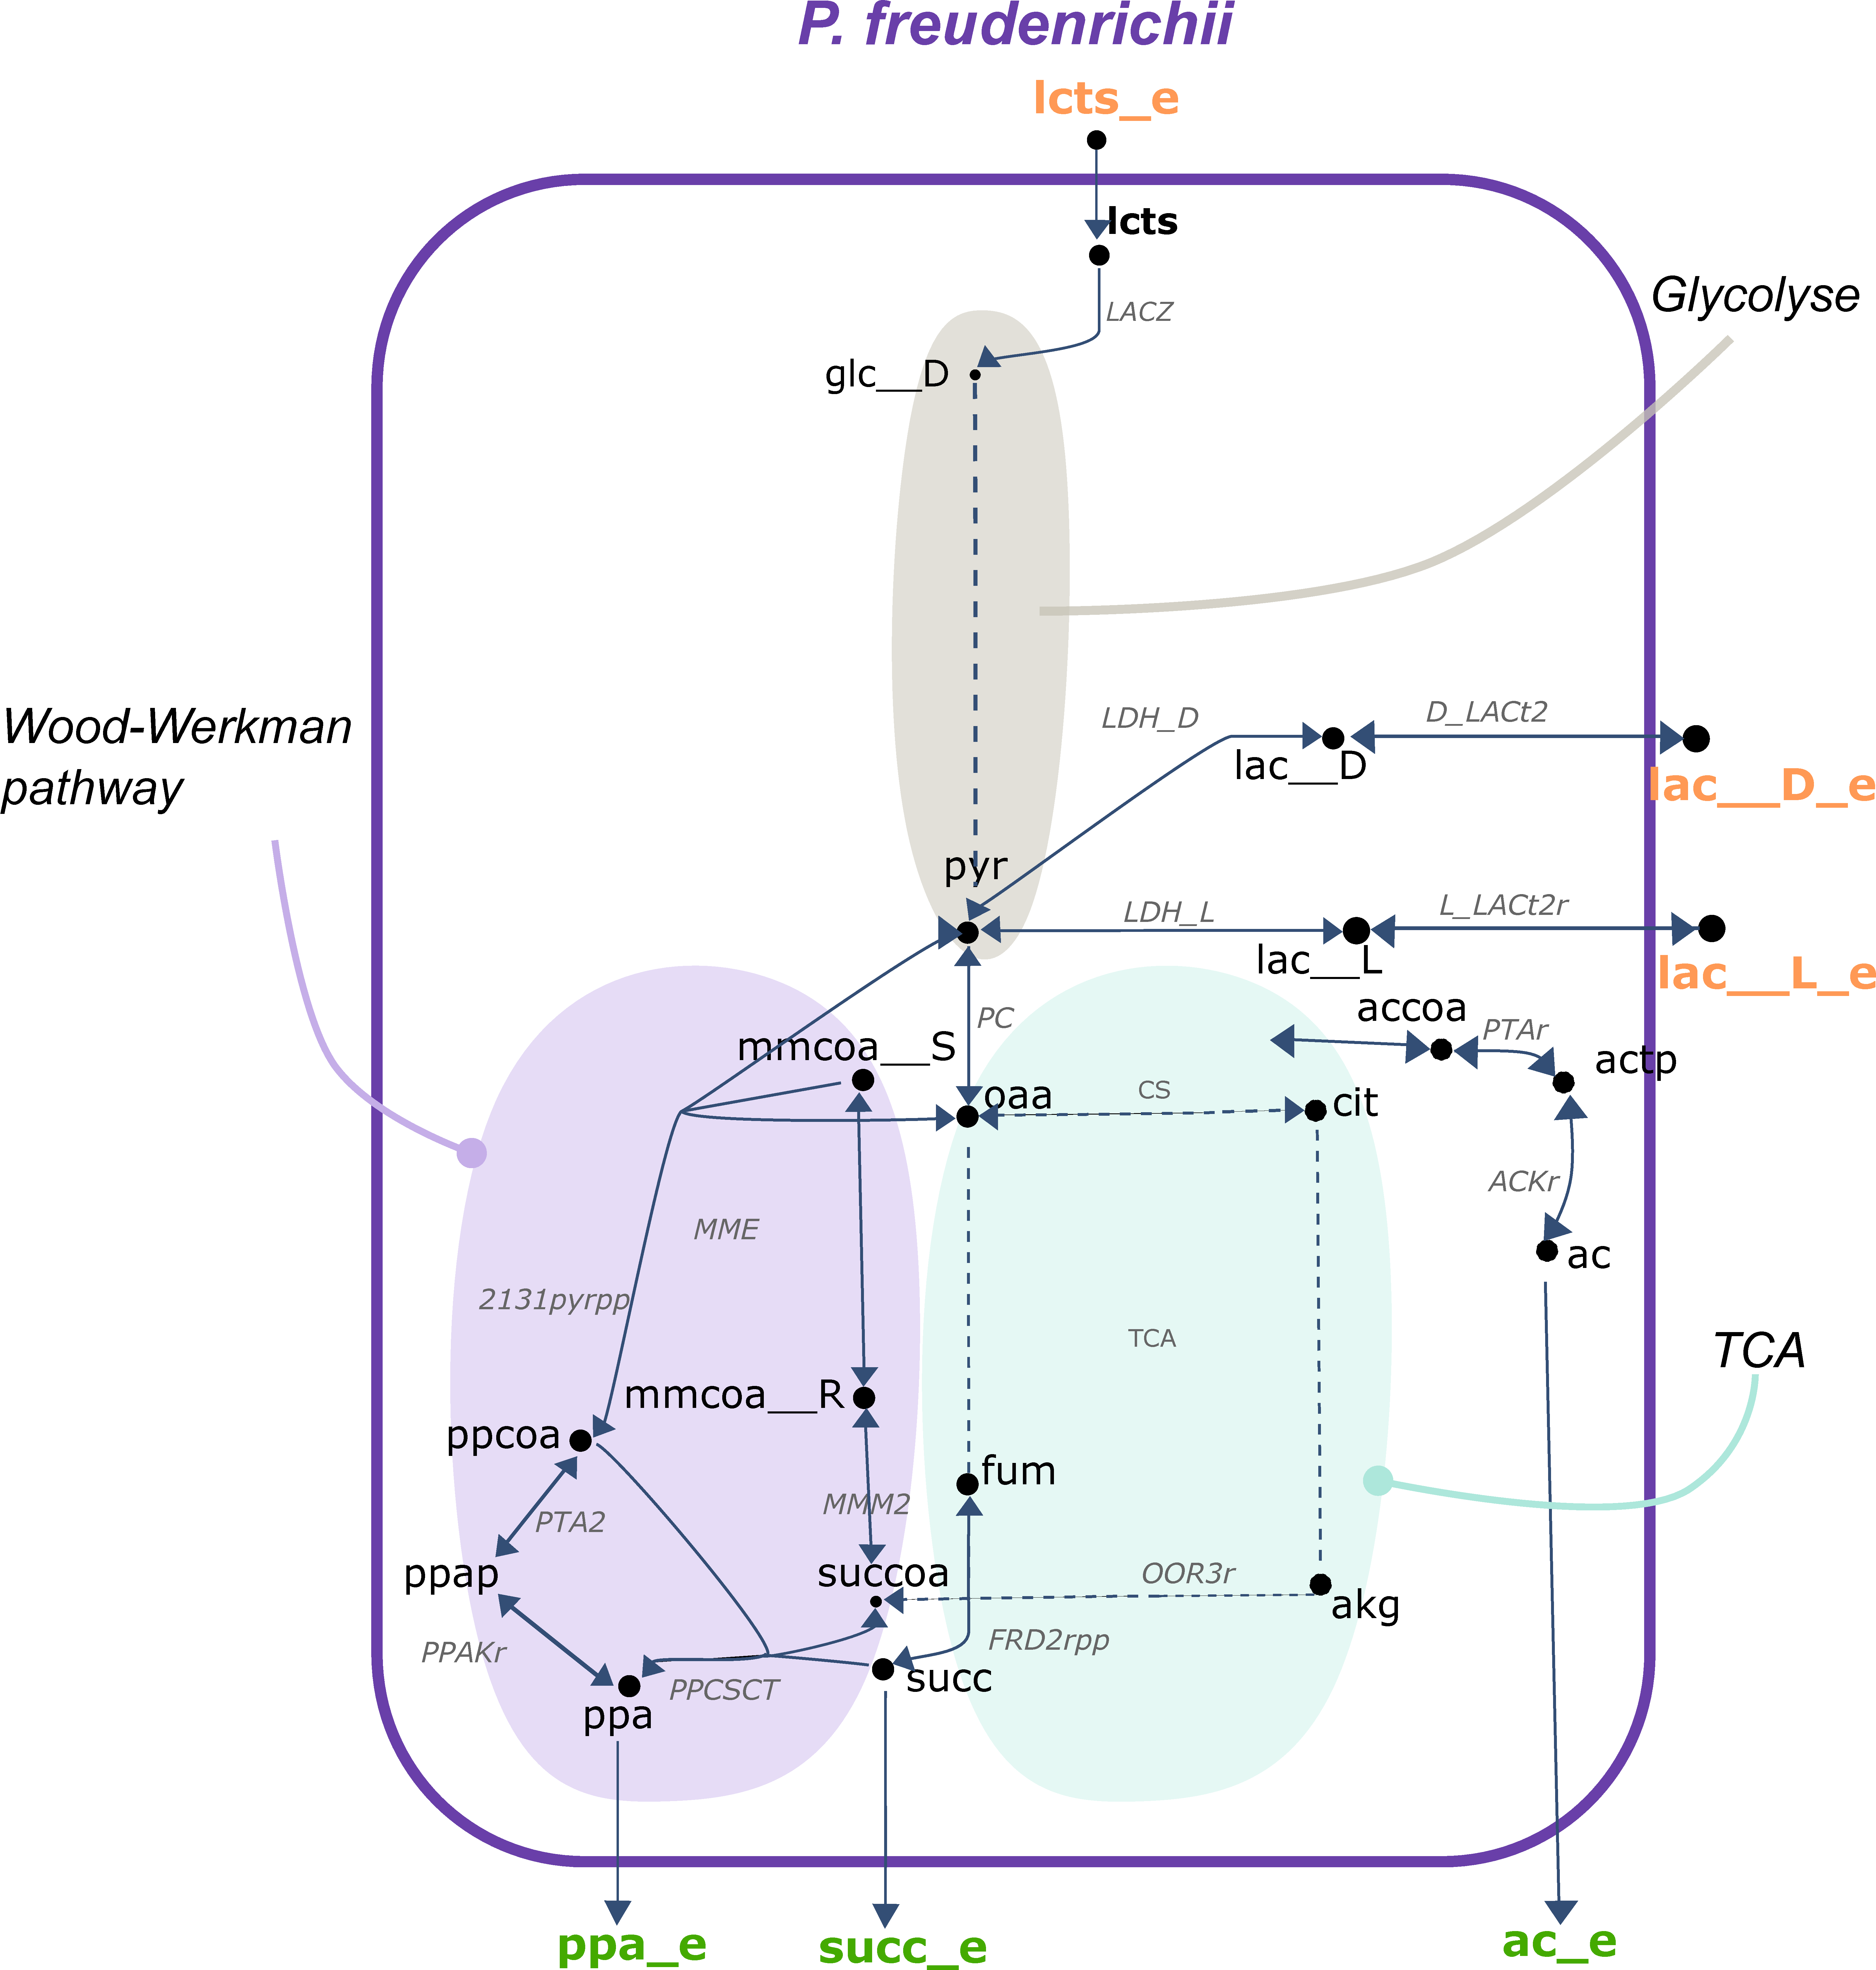
\includegraphics[width=1\textwidth]{img/tango/carte_freud.pdf}
    \caption{\textbf{Cartes des voies métaboliques du métabolisme carboné central  d'intérêt de \textit{P. freudenreichii}}. La voie métabolique de la glycolyse est représentée en gris, le cycle du TCA en bleu clair, et la voie de Wood-Werkman en violet. Les métabolites en orange et vert correspondent aux entrées et sorties des modèles métaboliques. La liste des métabolites et des réactions est répertoriée à la fin du chapitre à la section \ref{abbreviation-reac}}
    \label{figure:metabolic_map_freud}
\end{figure}



Nous avons par la suite vérifié la qualité de chaque réseau métabolique: une faible fraction de réactions universellement bloquées (< 3\%), et une faible fraction de réactions sans association de gène-proteine-réactions (GPR) (< 30\%) \citep{Lieven.2020}. Puis, nous les avons analysés par la méthode d'équilibre des flux (FBA) \citep{Palsson1994,Orth2010} assurant ainsi la production des molécules de la biomasse à partir de l'environnement nutritionnel du lait. Nous avons obtenu des taux de croissances allant de 0.187 $\text{mmol.gDW}^{-1}\text{.hr}^{-1}$ pour \freud à 2.17 $\text{mmol.gDW}^{-1}\text{.hr}^{-1}$ pour \lactis. Comme les conditions dans le fromage correspondent à des conditions de microaérobiose \citep{Miyoshi2003}, une attention particulière a été donnée au rôle de l'oxygène sur le métabolisme des trois bactéries en modifiant la borne supérieure de la réaction d'importation dans le compartiment cytosolique. Les caractéristiques générales des trois modèles sont décrites dans la Table \ref{tab:table1}. Nous observons que \lactis a un plus petit nombre de réactions que les deux autres souches, une différence qualitative qui est aussi observée pour les autres souches de la même espèce dans d'autres bases de données \citep{Noronha.2018}.\\


\begin{center}
    \begin{table}[h!]
    \begin{tabular}{|l|c|c|c|}
    \hline
                                                                                & \textit{P. freudenreichii} & \textit{L. plantarum} & \textit{L. lactis} \\ \hline
    Nombre de gènes                                                                                     & 1473                       & 1433                  & 1272               \\ \hline
    Nombre de métabolites                                                                               & 1284                       & 1045                  & 939               \\ \hline
    Nombre de réactions                                                                                 & 1790                       & 1523                  & 1337               \\ \hline
    \begin{tabular}[c]{@{}l@{}}Pourcentage de réactions\\  associées a au moins un gène \end{tabular} & 76.6                       & 79.0                    & 82.1               \\ \hline
    \begin{tabular}[c]{@{}l@{}}Taux de croissance en $\text{mmol.gDW}^{-1}\text{.hr}^{-1}$\end{tabular}                           & 0.187                       & 0.645                  & 2.172                \\ \hline
    \end{tabular}
    \caption{Caractéristiques générales des 3 modèles métaboliques}
    \label{tab:table1}
    \end{table}
\end{center}




\begin{table}[h!]
\begin{adjustbox}{width=1\textwidth}
\begin{tabular}{|c|c|c|c|c|}
\hline
GEM & Reaction & Bornes & Valeur & Justification \\
 \hline
 \TableBac{\lactis}{8} & \TableReac{ACTD2}{borne inférieure}{0}{borne supérieure}{0}{Permet l'activation de la voie métabolique de l'acetolactate}\\
 \cline{2-5}
 & \TableReac{ACLDC}{borne inférieure}{0}{borne supérieure}{2}{Permet l'activation de la voie métabolique de l'acetolactate}\\
 \cline{2-5}
 & \TableReac{ACLS}{borne inférieure}{2}{borne supérieure}{1000}{Permet l'activation de la voie métabolique de l'acetolactate}\\
 \cline{2-5}
 & \TableReac{LACZ}{borne inférieure}{0.0006}{borne supérieure}{2}{Oblige la consommation de lactose}\\ 
 \hline
 \TableBac{\plantarum}{10} & \TableReac{PFL}{borne inférieure}{0}{borne supérieure}{0}{Permet la production des deux isomères de lactate à partir du lactose} \\
 \cline{2-5}
 & \TableReac{LCTSt3ipp}{borne inférieure}{0}{borne supérieure}{0}{Redirige le flux de lactose dans la voie métabolique de la Glycolyse}\\
\cline{2-5}
 & \TableReac{ACTD2}{borne inférieure}{0}{borne supérieure}{0}{Permet l'activation de la voie métabolique de l'acetolactate}\\
 \cline{2-5}
 & \TableReac{GALUi}{borne inférieure}{-30}{borne supérieure}{10}{Permet la production des deux isomères de lactate à partir du lactose}\\
 \cline{2-5}
 & \TableReac{ACLS}{borne inférieure}{2}{borne supérieure}{1000}{Permet l'activation de la voie métabolique de l'acetolactate}\\
 \hline
 \TableBac{\freud}{14} & \TableReac{6PGALSZ}{borne inférieure}{0}{borne supérieure}{0}{Réaction appartenant à la voie du tagatose, non présente chez \freud} \\
 \cline{2-5}
 & \TableReac{XYLI2}{borne inférieure}{0}{borne supérieure}{0}{\begin{minipage}[t]{0.6\linewidth}A partir du glucose, le fructose était produit à la place du glucose-6-phosphate et la Glycolyse n'était pas activée.\end{minipage}}\\
\cline{2-5}
 & \TableReac{POX2}{borne inférieure}{0}{borne supérieure}{0}{Régule le flux d'acétate}\\
 \cline{2-5}
 & \TableReac{PPAKr}{borne inférieure}{0}{borne supérieure}{0}{Inhibe la surproduction de l'acétate}\\
 \cline{2-5}
 & \TableReac{LACZ}{borne inférieure}{0}{borne supérieure}{5}{Autorise la consommation de lactose}\\
  \cline{2-5}
 & \TableReac{PTAr}{borne inférieure}{-1000}{borne supérieure}{8}{Permet d'obtenir le bon ratio de production propionate/acetate}\\
  \cline{2-5}
 & \TableReac{2131pyrpp}{borne inférieure}{8}{borne supérieure}{1000}{Permet d'obtenir le bon ratio de production propionate/acetate}\\
\hline
\end{tabular}
\end{adjustbox}
\caption{\textbf{Raffinement manuel des GEMs avec les justifications correspondantes} \label{table:manual-refinement}}
\end{table}


Le raffinement des trois modèles FBA a permis la prédiction de production et de consommation de plusieurs composés d'arômes tels que les acides lactique, acétique et propionique, le diacétyl et le butanediol \citep{Smid2014, Cao2021} (Fig.~\ref{figure:metabolic_map_freud},\ref{figure:metabolic_map_lactis},\ref{figure:metabolic_map_plantarum}). De plus, les spécificités métaboliques de chaque souche en fonction de leur métabolisme primaire ont été reproduites fidèlement: la voie de Wood-Werkman pour \freud, la voie du tagatose pour \lactis et la voie de la transketolase pour \plantarum.  \\


La méthode itérative a permis de répondre à la première exigence que le modèle numérique doit satisfaire: "vérifier que les voies métaboliques d'intérêts  permettant la production des composés d'arômes soient présentes et activées". Nous avons reproduit de manière qualitative, la production et la consommation de métabolites connues de la littérature. Nous avons également prédit de nouveaux comportements métaboliques, comme la dégradation du citrate chez \plantarum par les enzymes de la famille CITL. Afin d'obtenir des prédictions numériquement proches des courbes de croissance et des concentrations de métabolites, nous avons ensuite calibré chaque modèle individuel.

\subsubsection*{Calibration dynamique}
Afin d'obtenir des modèles individuels suffisamment bien curés, nous avons utilisé les données cinétiques à disposition pour affiner chaque modèle (voir \ref{données-calibration}). Cette étape de calibration consiste à minimiser l'écart entre les données expérimentales et la simulation de façon dynamique en estimant des paramètres (voir \ref{table:manual-refinement}). Pour ce faire, le modèle numérique devait permettre: d'intégrer des données hétérogènes et de modéliser la dynamique de croissance et de production/consommation de métabolites pour chaque souche.

L'objectif à atteindre est de retrouver numériquement les observations biologiques que sont: la croissance bactérienne,  l'évolution du pH pour \lactis et \plantarum ainsi que les concentrations des métabolites pour \freud. \\

Pour estimer les paramètres, nous avons résolu le problème de minimisation décrit dans les équations \ref{eq:optim_LAB} pour les bactéries lactiques et \ref{eq:optim_freud} pour \freud. Brièvement, nous cherchons à minimiser l'écart aux données de croissance pour les 3 espèces, l'écart aux données de pH pour les deux bactéries lactiques et l'écart aux données de dosage de métabolites pour \freud. Avec ce type de méthode, le sur-apprentissage, est une problématique à prendre en compte. Afin de l'éviter, nous avons optimisé un petit nombre de paramètres pour chaque espèce : seulement deux paramètres ont été utilisés pour calibrer la croissance de \lactis et la régulation du pH, trois pour \plantarum régulant le pH ainsi que sa croissance, et enfin, un paramètre pour \freud, ajustant sa croissance.\\

Ce principe de calibration des modèles se base également sur un processus itératif induit par les allers-retours entre les données simulées et les paramètres inférés. En effet, la solution informatique d'optimiser des paramètres pour ajuster les modèles n'est pas suffisante. Nous avons dû établir des contraintes de modélisation dynamique en se basant sur la connaissance biologique de l'espèce ainsi que sur les résultats des simulations. Expérimentalement, nous avons observé que le métabolisme des bactéries lactiques est toujours actif pendant la phase stationnaire au regard de la courbe de pH, indiquant que les bactéries continuent d'acidifier. Elles peuvent ainsi continuer de produire du lactate et de l'acétate à partir du lactose puisque ce dernier n'est pas considéré comme limitant dans les conditions expérimentales. La première contrainte dynamique a consisté à réguler le flux de production des acides lactique et acétique par le flux de consommation du lactose, source de carbone principale. 

\paragraph*{\lactis et \plantarum}
Pour moduler le flux de production des acides lactique, les bornes supérieures des réactions d'échange du lactate EX\_lac\_\_L\_e et EX\_lac\_\_D\_e, sont modulées comme suit:

\begin{equation}
min(\frac{m_{lcts_e}}{\Delta t*\sum_{i \in \mathcal{M}(lcts_e)} b_i},\mu_{max,lcts}*10^{(-k_{lac}*\phi_{undiss})}+\mu_{min,lcts})*4
\label{eq:lactate_lactis}
\end{equation}

Toutes les constantes sont décrites dans la sous section \ref{dynamic analyse}. Pour rappel, $m_{lcts_e}$ est la concentration du lactose, $\mathcal{M}(lcts_e)$ le sous ensemble des bactéries métabolisant le lactose, $\mu_{max,lcts}$ et $\mu_{min,lcts}$ valeurs maximales et minimales de consommation du lactose, $k_{lac}$ une décroissance exponentielle et $\phi_{undiss}$ la fonction qui calcule la concentration de la forme non dissociée de l'acide lactique à partir du lactate.

Comme la production de lactate est reliée à la disponibilité du lactose, nous avons modulé dynamiquement l'export de lactate en fonction de la quantité de lactose à importer, avec un coefficient st\oe{}chiométrique de 4 (voir eq.~\eqref{eq:lactose_lab}). Ce coefficient permet de mieux ajuster la courbe de production de lactate aux données expérimentales.\\

Étant donné que l'acétate n'est pas relié dans notre modèle au calcul du pH, mais est produit à partir du lactose par l'intermédiaire du pyruvate, nous avons appliqué une simple régulation de la production de l'acétate par la quantité de lactose disponible. Soit EX\_ac\_e, la réaction d'échange de l'acétate, sa borne supérieure sera modulée dynamiquement par:

\begin{equation*}
max(-\frac{m_{lcts_e}}{\Delta t*\sum_{i \in \mathcal{M}(lcts_e)} b_i},v^{exp}_{i,ac_e})
\end{equation*}

La production d'acétate est régulée par la disponibilité de lactose quand celui ci est épuisé, représenté par $-\frac{m_{lcts_e}}{\Delta t*\sum_{i \in \mathcal{M}(lcts_e)} b_i}$ , autrement sa production sera limitée par sa limite d'export physiologique intrinsèque $v^{exp}_{i,ac_e}=0.5$ pour \lactis et $v^{exp}_{i,ac_e}=1.0$ pour \plantarum. \\

Lorsque les concentrations extra-cellulaires de lactose sont suffisamment importantes, le flux de consommation du lactose par les bactéries lactiques est également régulé par l'acidité libérée par ces bactéries: $-\mu_{max,lcts}*10^{(-k_{lac}*\phi_{undiss})}-\mu_{min,lcts}$. En effet, le métabolisme des bactéries lactiques continue même lorsqu'elles sont à l'état stationnaire. En revanche, lorsque la concentration de lactose devient insuffisante, un partage uniforme entre les bactéries consommatrices, composées des deux bactéries lactiques et de la bactérie propionique est mis en place: $-\frac{m_{lcts_e}}{\Delta t*\sum_{i \in \mathcal{M}(lcts_e)} b_i}$. L'approche modélisant ce processus est inspirée des travaux de \citep{Ozcan.2020} dans lesquelles l'acidité libérée par les bactéries lactiques est représentée par le forme non dissociée de l'acide lactique.\\

Soit EX\_lcts\_e, la réaction d'échange du lactose. Sa borne inférieure des bactéries lactiques sera modulée dynamiquement par:

\begin{equation}
max(-\frac{m_{lcts_e}}{\Delta t*\sum_{i \in \mathcal{M}(lcts_e)} b_i},-\mu_{max,lcts}*10^{(-k_{lac}*\phi_{undiss})}-\mu_{min,lcts})
\label{eq:lactose_lab}
\end{equation}

Concernant la régulation par le pH, la quantité d'acide lactique non dissocié est calculé à partir de la concentration de lactate au moyen de la fonction $\phi_{undiss}$ (voir équation \ref{eq:undissociated-lactate} pour l'expression de cette fonction); puis, avec une croissance exponentielle à partir de la valeur $-\mu^{lact}_{max,lcts}-\mu^{lact}_{min,lcts}$ (respectivement $-\mu^{plant}_{max,lcts}-\mu^{plant}_{min,lcts}$ pour \plantarum) à la valeur $-\mu^{lact}_{min,lcts}$ ($-\mu^{plant}_{min,lcts}$) quand la concentration d'acide lactique non dissocié augmente, avec un taux exponentiel $k_{lac}$. Les valeurs de $\mu^{lact}_{max,lcts}$ (resp. $\mu^{plant}_{max,lcts}$), $\mu^{lact}_{min,lcts}$ (resp.$\mu^{plant}_{min,lcts}$) et $k_{lac}$ sont inférées à partir des expériences de co-cultures. \\


Pour \freud, lorsque le lactose est épuisé numériquement, nous avons appliqué le même partage uniforme des ressources que pour les bactéries lactiques : $-\frac{m_{lcts_e}}{\Delta t*\sum_{i \in \mathcal{M}(lcts_e)} b_i}$. Sinon, comme il n'est pas impacté par sa propre acidification, un flux constant $F_{lcts}$ estimé des données de métabolomiques en culture pure est appliqué lorsque la quantité de lactose est suffisamment abondante. Ce flux constant est estimé de la façon suivante:
\begin{equation}
\label{sec:estimate-bounds-freud}
 {\mu}_{i,j} = \alpha \frac{ m_j(T)-m_j(0)}{\int_0^T b_i(t) dt}
\end{equation}
 
où ${\mu}_{i,j}$ correspond à la valeur de flux,  $m_j$ la concentration du métabolite, $T$ valeur finale, $0$ valeur initiale, $b_i(t)$ la densité bactérienne, et $\alpha$, un coefficient prenant en compte les erreurs d'approximation.


%Concernant \freud, lorsque le concentration de lactose est épuisé nous avons appliqué le même partage uniforme que pour les bactéries lactiques: $-\frac{m_{lcts_e}}{\Delta t*\sum_{i \in \mathcal{M}(lcts_e)} b_i}$. 


La borne supérieure du lactose pour chaque bactérie reste inchangée. \\

%Nous avons utilisé jusqu'ici uniquement la connaissance apportée par la littérature afin de contraindre chaque modèle individuel en y associant une équation de régulation. Dans les paragraphes suivants, une communication entre les données et les modèles sera utilisée afin d'ajouter des contraintes et expliquer les données observées pour chaque souche.\\ 

Pour rappel, le lactate, l'acétate, le succinate et le propionate sont dosés pour \freud et les concentrations initiales et finales sont récupérées. Ainsi, les bornes des flux de production de ces composés sont estimées à partir des données dans le but de rapprocher la valeur de flux de production prédite par le modèle avec celle des données expérimentales. Dans ces conditions expérimentales, les nutriments ne sont pas considérés comme limitant, ainsi nous avons modéliser la phase plateau par une croissance logistique. \\

Pour \freud, la borne de consommation du lactate est modélisée comme suit:

\begin{equation}max(-\frac{m_{lac_{L,e}}}{\Delta t*\sum_{i \in \mathcal{M}(lac_L)} b_i},F_{lac}*K_{freud}* \frac{b_{freud}}{B_{p,freud}}) \label{eq:optim-K-lac}\end{equation}

Comme précédemment avec le lactose, lorsque la quantité de lactate est insuffisante, nous avons utilisé un partage uniforme des ressources $-\frac{m_{lac_{L,e}}}{\Delta t*\sum_{i \in \mathcal{M}(lac_L)} b_i}$ parmi les bactéries consommatrice du lactate $\mathcal{M}(lac_L)$. Dans le cas contraire, un flux $F_{lac}$ estimé des données de métabolomiques en culture pure (voir l'équation \ref{sec:estimate-bounds-freud}) est appliqué après une régulation par la fraction $\frac{b_{freud}}{B_{p,freud}}$, où $B_{p,freud}$ est la valeur plateau de la concentration de la biomasse en pure culture, et $b_{freud}$ et la densité de biomasse actuelle, et le facteur $K_{freud}$, qui est inféré des données de croissance en culture pure. Cette modulation modélise un ordre de grandeur différent du rendement du métabolisme en culture pure ou en co-culture.

Comme l'acétate, le propionate et le succinate ne sont pas consommés par aucun des modèles métaboliques, seule la borne supérieure (de production) est modulée. Soient les réactions d'échanges d'acétate (EX\_ac\_e), de propionate (EX\_ppa\_e) et de succinate (EX\_succ\_e), la valeur de la borne supérieure est égale à:

\[F_{i}*K_{freud}* \frac{b_{freud}}{B_{p,freud}}, \quad \text{ pour } i \in \{\text{ EX\_ac\_e, EX\_ppa\_e,EX\_succ\_e} \}\]

où le taux maximal de production est défini par $F_{i}$, pour $i \in \{\text{ EX\_ac\_e,  EX\_ppa\_e,} $
$\text{ EX\_succ\_e} \}$ estimé à partir des données de métabolomique de culture pure (voir la section \ref{sec:estimate-bounds-freud}). Le même terme de modulation que dans l'équation \ref{eq:optim-K-lac} est appliqué, modélisant un un ordre de grandeur différent du rendement du métabolisme en culture pure ou en co-culture.\\

Cette étape itérative de calibration dynamique est coûteuse en temps. En effet, pour chacune des nouvelles valeurs de paramètres, nous avons lancé une simulation dynamique de chaque souche optimisée. 

Pour les autres métabolites suivis dynamiquement, c'est à dire le butanediol, le diacétyle et le citrate, la borne inférieure est modulée selon le principe de partage équitable décrit plus haut lorsque la quantité de substrat devient insuffisante.

Soient EX\_diact\_e, EX\_btd\_RR\_e et EX\_cit\_e les réactions d'échanges correspondantes aux diacétyle, butanediol et citrate, leurs bornes inférieures sont ainsi modulées par:

\begin{align*}
&max(-\frac{m_{j}}{\Delta t*\sum_{i \in \mathcal{M}(j)} b_i},v^{int}_{i,j})\\
&\text{ pour }i=\text{\lactis si } j \in \{EX\_diact\_e,EX\_btd\_RR\_e,EX\_cit\_e,EX\_ac\_e\}\\
&\text{ pour }i=\text{\plantarum si } j \in \{EX\_btd\_RR\_e\}
\end{align*}

%Limitation dynamique de consommation (voir eq. \eqref{eq:usual-consumption-limitation}). 
Quand le substrat n'est pas limité, l'import est contraint par la limite physiologique intrinsèque modélisé par $v^{int}_{i,j} = -8$ pour $j=$\lactis et $j \in \{EX\_diact\_e,EX\_btd\_RR\_e\}$,
$v^{int}_{i,j} = -1$ pour $j=EX\_cit\_e$ et $v^{int}_{i,j} = -5$ pour $i=\plantarum$ et $j \in \{EX\_ac\_e,EX\_btd\_RR\_e\}$ ou sinon, par la disponibilité du substrat uniformément partagé par les micro-organismes consommateurs: $-\frac{m_{j}}{\Delta t*\sum_{i \in \mathcal{M}(j)} b_i}$.\\

% Limitation dynamique de consommation usuelle (voir eq. \eqref{eq:usual-consumption-limitation}) Quand le substrat est pas limité, l'import est contraint par la limite physiologique intrinsèque modélisé par $v^{int}_{i,j} = -5$ pour $i=\plantarum$ et $j \in \{EX\_ac\_e,EX\_btd\_RR\_e\}$ et autrement, par la disponibilité du nutriment. La disponibilité du substrat est uniformément partagé par les micro-organismes consommateurs.
% \paragraph*{\lactis}
% \begin{itemize}
% \ReacListItem{EX\_diact\_e, EX\_btd\_RR\_e, EX\_cit\_e}{inférieur}
% {
% \begin{align*}
% &max(-\frac{m_{j}}{\Delta t*\sum_{i \in \mathcal{M}(j)} b_i},v^{int}_{i,j})\\
% &\text{ pour }i=\text{\lactis et }j \in \{EX\_diact\_e,EX\_btd\_RR\_e,EX\_cit\_e,EX\_ac\_e\}
% \end{align*}
% }
% {supérieure}
% {1000}
% {
% }

% \end{itemize}

% \paragraph*{\plantarum}
% \begin{itemize}
%     \ReacListItem{EX\_btd\_RR\_e}{inférieur}{
% \begin{align*}
% &max(-\frac{m_{j}}{\Delta t*\sum_{i \in \mathcal{M}(j)} b_i},v^{int}_{i,j}), \\
% &\text{ pour } j=\text{\plantarum et } j \in \{EX\_btd\_RR\_e\}
% \end{align*}
% }
% {supérieure}
% {1000}
% {


% }

% \end{itemize}

En plus de ces régulations dynamiques, nous avons observé \textit{via} la méthode de FVA un flux important de consommation du citrate, de la serine, du glutamate et de l'alanine, empêchant d'obtenir la précision numérique des composés dosés en culture pure. Ainsi, pour réorienter les flux dans les voies métaboliques attendues nous avons réduit chacune des bornes d'importation de ces composés à -12, améliorant les prédictions. \\

Toutes ces modifications faites, soit à partir des connaissances biologiques soit à partir des données biochimiques, rendent la prédiction des modèles plus précise et plus fidèle aux données. \\

\subsubsection*{Simulation des modèles calibrés}

Nous avons ainsi curé manuellement et calibré dynamiquement chacun de nos modèles FBA individuels dans le but premier de retrouver les valeurs de concentration des expériences biologiques en culture pure. Les simulations statiques et dynamiques de nos modèles calibrés sont représentées dans les Figures ~\ref{dfba_metabolite_lactis}, \ref{dfba_metabolite_plant} et \ref{dfba_metabolite_freud}. Chaque sous figure (a) représente les flux des voies métaboliques d'intérêt calculés par le FBA lors de l'inoculation alors qu'aucun métabolite n'est limitant. \\

Le modèle FBA de \lactis (figure ~\ref{dfba_metabolite_lactis}a), nous montre une préférence d'utilisation de la voie métabolique du tagatose plutôt que de Leloir pour dégrader le lactose. Nous remarquons également que les deux isomères du l'acide lactique sont produits \textit{via} la voie de la glycolyse avec un plus grand flux de production pour le D-lactate, expliquant ainsi l'acidification du lait et du caillé durant le processus de fabrication de fromage.(Fig. \ref{dfba_metabolite_lactis}a). Concernant la voie de l'acétolactate, nous remarquons qu'elle est bien active grâce à la production du diacétyl et du butanediol. Enfin, nous observons également un flux de consommation du citrate, \textit{via} la réaction $CITL$ encodée par le gène $citL$. \\

\begin{figure}[h!]
    \centering
    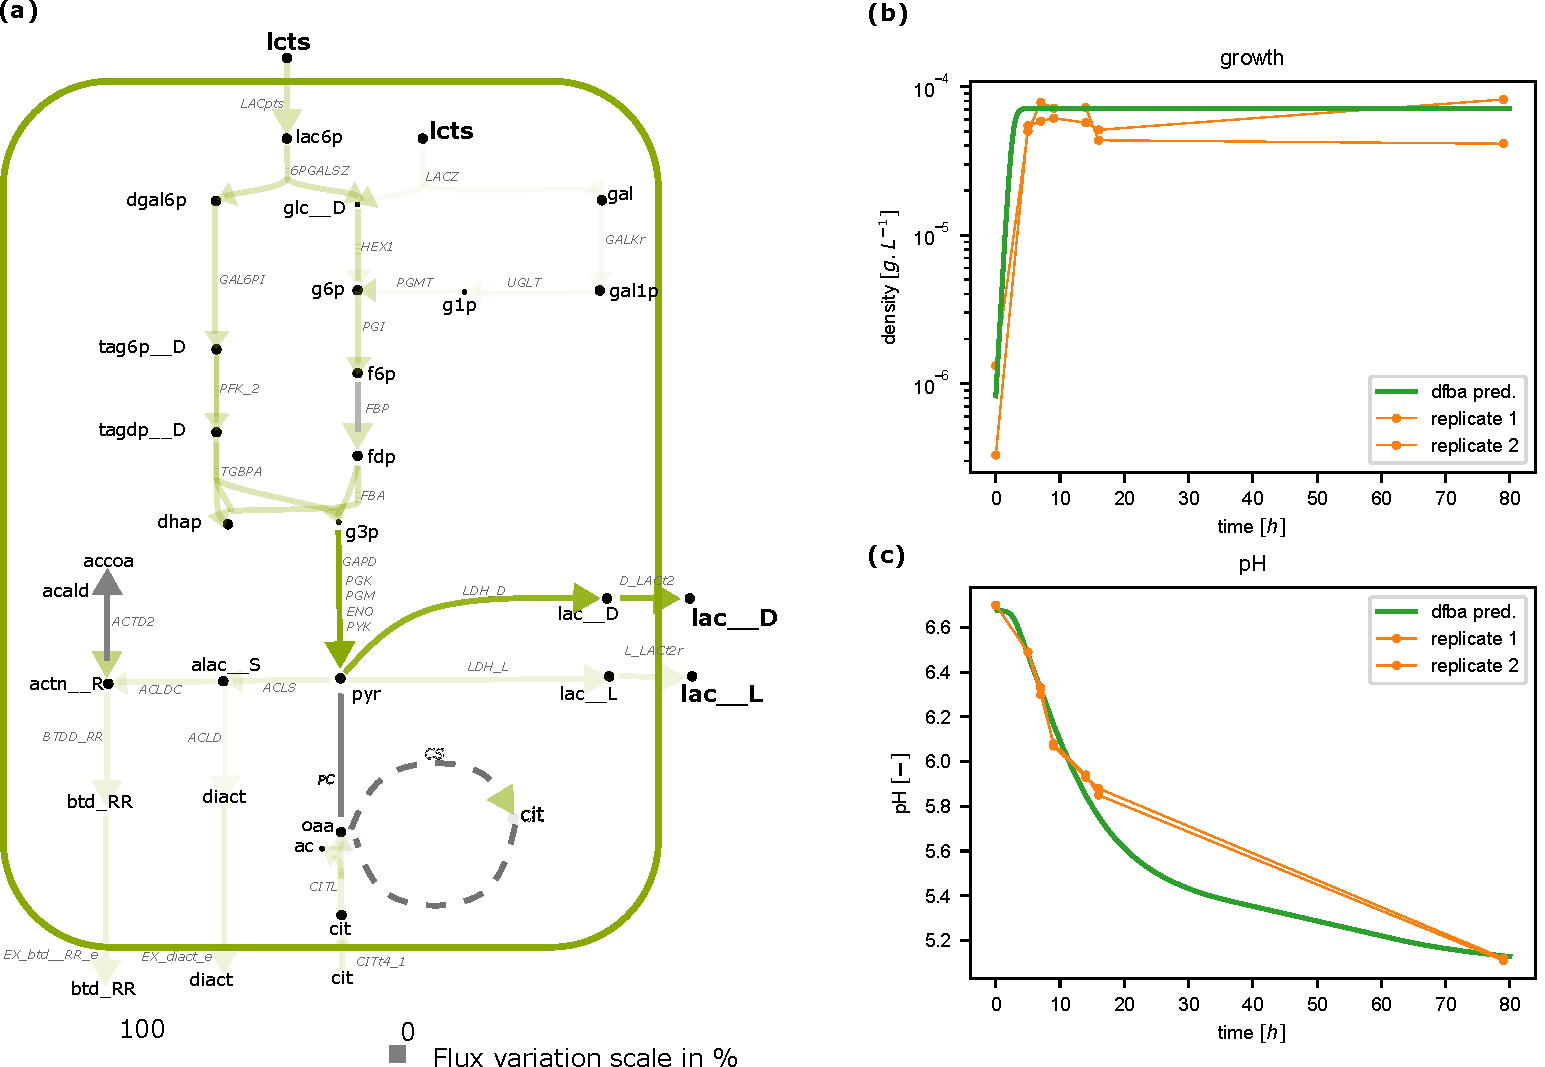
\includegraphics[width = 1\textwidth]{img/tango/FIG2_opt_explo_ll.pdf}
    \caption{\textbf{ Réseau métabolique de \lactis après calibration sur les données de culture pure.} (a) Représentation d'un FBA appliqué sur le métabolisme carboné central lors de l'inoculation de \lactis. L'échelle de couleur représente les valeurs de flux prédites par le FBA et normalisées par la plus haute valeur de flux prédites sur les voies métaboliques illustrées. (b) Simulation de la croissance de \lactis au cours du temps après inférence des paramètres dans le modèle (courbe verte) et d'après les données expérimentales (courbe orange, with $\pm 1/4$ log, which is the admitted range of precision for plating numbering). (c) Courbes de pH dans des conditions de culture pure simulé par le modèle (courbe verte) et issues des données expérimentales (croix orange , with standard deviation). La liste des métabolites et des réactions est répertoriée à la fin du chapitre à la section \ref{abbreviation-reac}}
    \label{dfba_metabolite_lactis}
\end{figure}

Contrairement à \lactis, le modèle métabolique de \plantarum semble avoir une préférence de production pour le lactate, montrant ainsi sa contribution à l'acidification du fromage. La voie de la glycolyse est active, ainsi que la consommation du lactose jusqu'à la production des deux formes du lactate. Nous remarquons également un flux de production de l'acide acétique par la voie de l'acétatekinase, contribuant plus faiblement à l'acidification (Fig. \ref{figure:metabolic_map_plantarum}). Les simulations dynamiques de \plantarum ont montré une activation des voies fermentaires hétérolactique et homolactique. Cependant à notre connaissance, la voie métabolique de la transkétolase, représentant la fermentation hétérolactique, est observée pour la première fois dans un contexte laitier. La consommation du citrate est connue pour être dépendante de la souche au sein de l'espèce \plantarum \citep{Palles1998}. Elle a été observée dans notre cas à travers la réaction de transport $FEDCabc$, conduisant à une augmentation de la quantité de pyruvate intracellulaire. \\

\begin{figure}[h!]
    \centering
    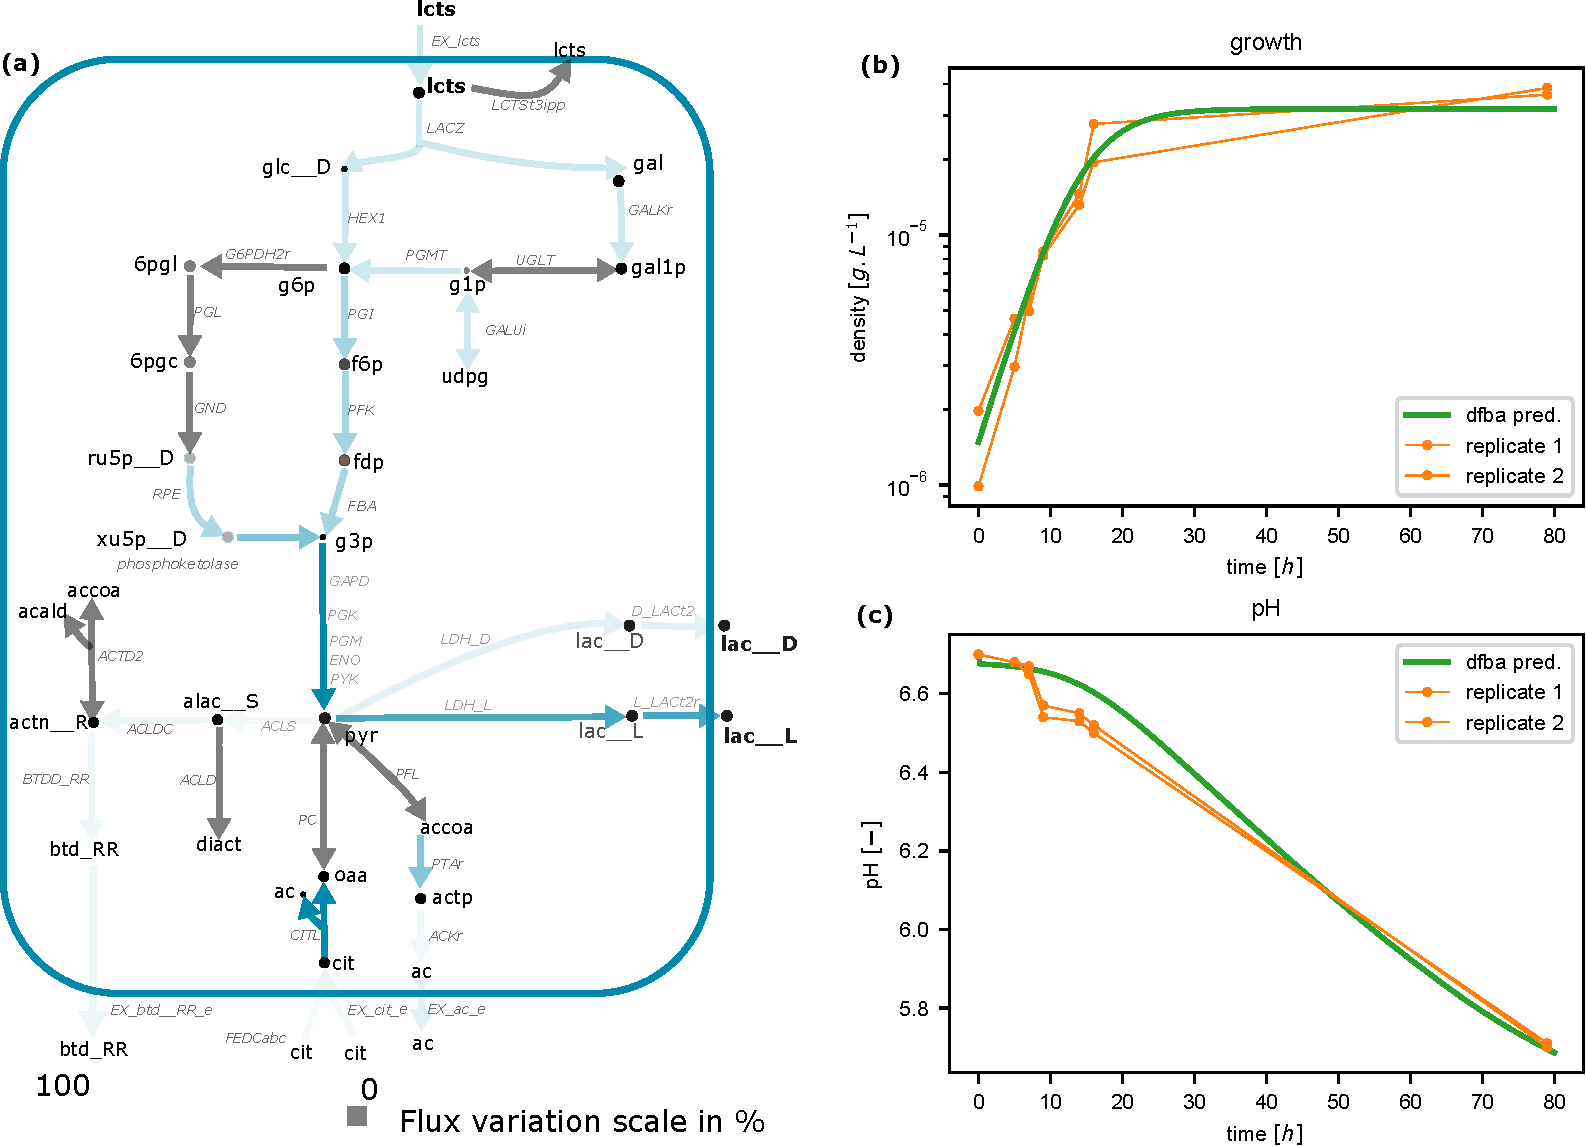
\includegraphics[width = 1\textwidth]{img/tango/FIG3_opt_explo_lp.pdf}
    \caption{\textbf{Réseau métabolique de \plantarum après calibration sur les données de culture pure.} (a) Représentation d'un FBA appliqué sur le métabolisme carboné central lors de l'inoculation de \plantarum. L'échelle de couleur représente les valeurs de flux prédites par le FBA et normalisées par la plus haute valeur de flux prédites sur les voies métaboliques illustrées. (b) Simulation de la croissance de \plantarum au cours du temps après inférence des paramètres dans le modèle (courbe verte) et d'après les données expérimentales (courbe orange, with $\pm 1/4$ log, which is the admitted range of precision for plating numbering). (c) Courbes de pH dans des conditions de culture pure simulé par le modèle (courbe verte) et issues des données expérimentales (croix orange , with standard deviation). La liste des métabolites et des réactions est répertoriée à la fin du chapitre à la section \ref{abbreviation-reac}}
    \label{dfba_metabolite_plant}
\end{figure}

 
Enfin, le modèle FBA de \freud consomme préférentiellement du lactose malgré la présence de l'acide lactique (Fig. \ref{dfba_metabolite_freud}a). Cependant, nous retrouvons une activation simultanée des cycles du TCA et de Wood-Werkman \citep{Deborde2000}, le premier permettant la régénération des sources de carbone nécessaires pour l'activation du second et ainsi, la production de propionate.

\begin{figure}[htpb!]
    \centering
    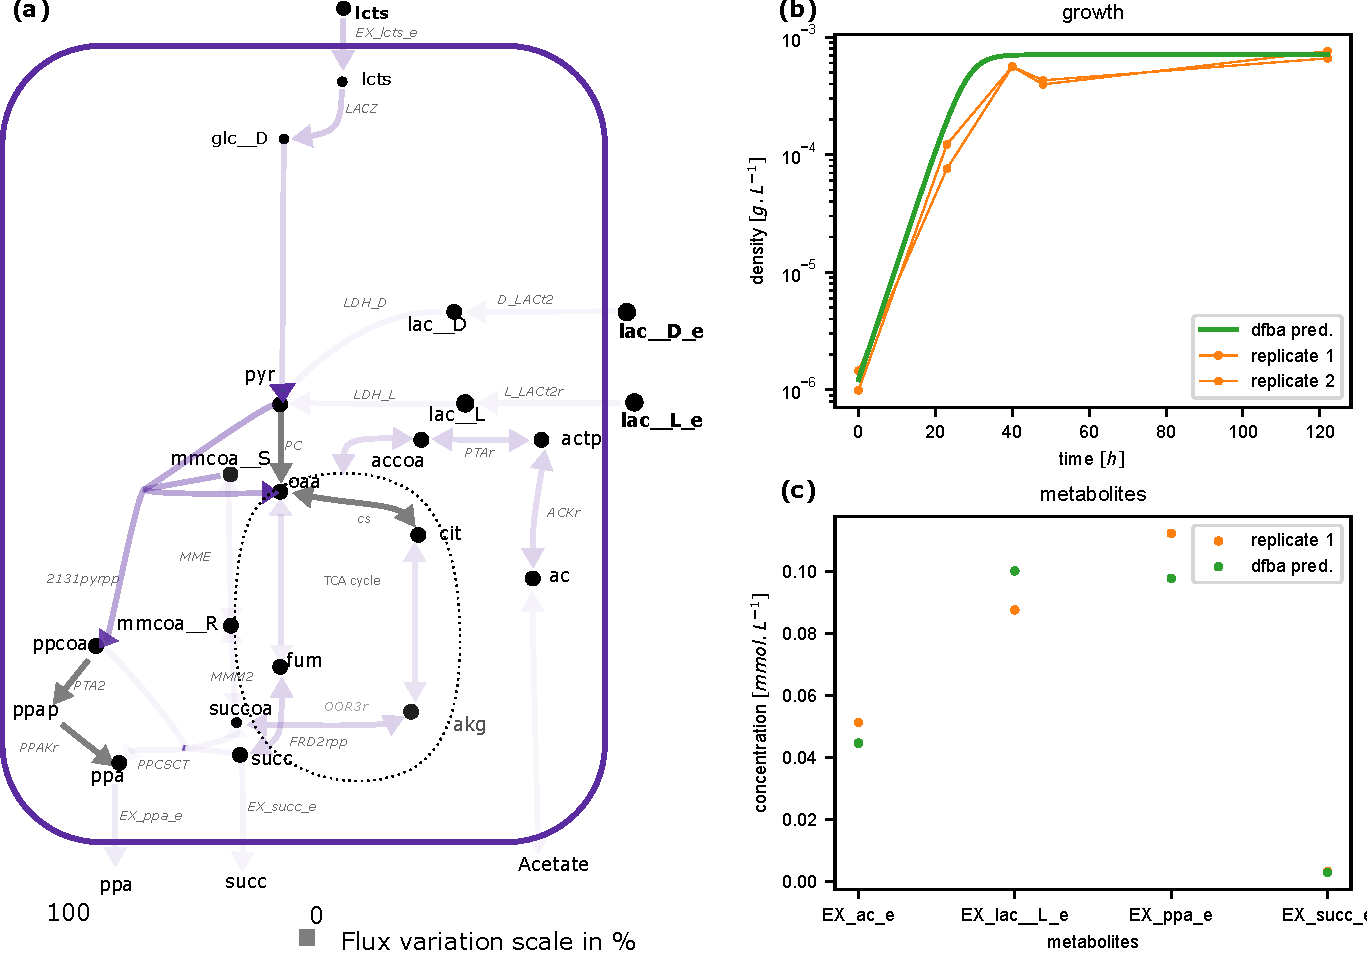
\includegraphics[width = 1\textwidth]{img/tango/FIG4_opt_explo_pf.pdf}
    \caption{\textbf{Réseau métabolique de \freud après calibration sur les données de culture pure.} (a) Représentation d'un FBA appliqué sur le métabolisme carboné central lors de l'inoculation de \freud. L'échelle de couleur représente les valeurs de flux prédites par le FBA et normalisées par la plus haute valeur de flux prédites sur les voies métaboliques illustrées. (b) Simulation de la croissance de \freud au cours du temps après inférence des paramètres dans le modèle (courbe verte) et d'après les données expérimentales (courbe orange, with $\pm 1/4$ log, which is the admitted range of precision for plating numbering). (c) Concentrations de lactate, acetate, propionate et succinate simulées (points verts) observées (croix en orange avec un écart-type) au temps final. La liste des métabolites et des réactions est répertoriée à la fin du chapitre à la section \ref{abbreviation-reac}
    }
    \label{dfba_metabolite_freud}
\end{figure}


Les sous figures (b) des Figures \ref{dfba_metabolite_lactis},\ref{dfba_metabolite_plant},\ref{dfba_metabolite_freud} montrent que les courbes de croissance simulées (en vert) sont fidèles aux données de croissances expérimentales de chaque souche microbienne. Concernant le pH, pour les sous figures~\ref{dfba_metabolite_lactis}, \ref{dfba_metabolite_plant} (c), nous avons observé que l'utilisation de la concentration du lactate dans une approximation du pH permet d'expliquer le pH observé lors des cultures pures de \lactis et \plantarum. Enfin, notre modèle métabolique de \freud retrouve les concentrations finales prédites par les expériences biologiques (Figure \ref{dfba_metabolite_freud}(c)). Afin de vérifier statistiquement que l'apprentissage de nos modèles est correct, nous avons représenté sur la figure Fig.~\ref{fig:qqplot} (a) les valeurs de croissance, de pH et de métabolites calculés par notre modèle et celles des données expérimentales. Nous observons une très bonne corrélation avec une valeur de $\text{R}^2$ = 0.99, montrant ainsi que nos modèles métaboliques individuels sont suffisamment bien ajustés. \\

\begin{figure}[h!]
    \centering
    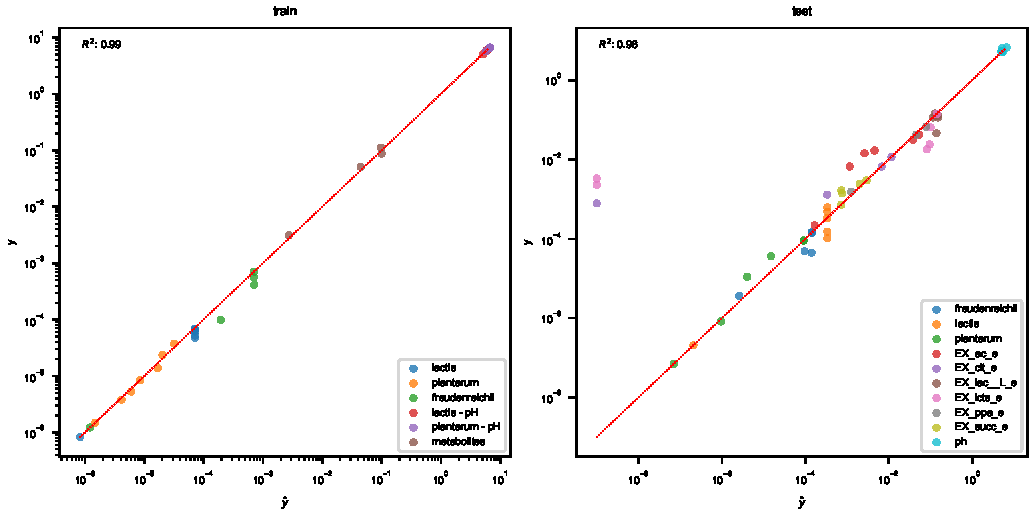
\includegraphics[width = 1\textwidth]{img/tango/qqplot.pdf}
    \caption{\textbf{Validation des prédictions après apprentissage.} Les valeurs simulées issues des modèles ($\hat{y}$) et celles des données expérimentales respectives ($y$) lors de la phase d'apprentissage sur les données de cultures pures (a) et lors de la phase de test en communauté (b). La couleur représente le type de la donnée et la bissectrice est affichée par une ligne en pointillée rouge. Le $R^2$ est calculé selon la formule suivante : $R^2 = 1 - \frac{\sum_i (y_i - \hat{y}_i)^2)}{\sum_i (y_i - \bar{y}_i)^2)}$ où $\bar{y}$ est la valeur moyenne de $y$. Nous pouvons observer une bonne capacité du modèle à prédire les concentrations.}
    \label{fig:qqplot}
\end{figure}

Nous venons de voir tout le processus d'itération statique et dynamique nécessaire pour obtenir des modèles métaboliques complets et des prédictions numériquement fiables. L'étape finale pour la construction d'un modèle numérique explicatif du fonctionnement de cette communauté fromagère est de passer à l'échelle en créant un modèle de communauté afin de prédire les croissances de chaque souche en communauté, et dans un deuxième temps, d'explorer les interactions bactériennes potentielles et les contributions de chaque souche pour la production et la consommation de métabolites.

\subsection{Simulations à l'échelle de la communauté}
En premier lieu, nous avons créé un modèle de communauté où chaque espèce maximise sa propre biomasse et avons utilisé les modèles calibrés sur les données de cultures pures pour construire ce modèle.
Nous avons ensuite ajusté la valeur du "quorum sensing", correspondant à la valeur à laquelle nous observons une phase plateau, de chaque modèle individuel en intégrant la valeur de "quorum sensing" des données expérimentales en co-culture (voir la Table \ref{com_data} et l'équation \ref{eq:logistic-growth} dans le but de reproduire le comportement métabolique de la communauté \textit{in silico} (voir eq.~\ref{eq:system_dynamics_b}-\ref{eq:system_dynamics_m}). Ce modèle de communauté n'a subi aucun processus de calibration sur les nouvelles données, c'est à dire, aucun paramètre basé sur la métabolomique ou sur les données de croissance en co-culture n'a été utilisé afin d'affiner les prédictions. Ces données vont en revanche être consacrées à la validation des prédictions du modèle.

Les simulations de la croissance, du pH et de la métabolomique du modèle de communauté ont correctement expliqué les valeurs expérimentales (Fig. \ref{dfba_community}(a)-(c), Table supplémantaire \ref{table:co-culture-data}). Nous avons remarqué cependant une légère surestimation de la croissance de \freud durant la phase exponentielle. Concernant la prédiction des concentrations de métabolites issus de la métabolomique, nous avons observé une consommation plus lente du lactose tandis que celle du citrate s'ajuste bien avec les données expérimentales. La production de lactate est légèrement sur-prédite durant la phase exponentielle résultant d'une sur-acidification du fromage durant les étapes de moulage et de démoulage. En revanche, la production d'acétate est sous-prédite durant les premières phases de la fabrication du fromage, mais le taux de production pendant la maturation est correctement modélisé. Les courbes du propionate, et dans une moindre mesure, celle du succinate sont prédites avec précision par le modèle suggérant que la production de composés organoleptiques par \freud est correctement capturée. De plus, les voies métaboliques activées en mono-cultures le sont également en co-culture (Figure \ref{fig:switch_metabolic_pathway}). Enfin, afin de valider statistiquement les prédictions du modèle en communauté, nous avons fait une régression entre les valeurs prédites par le modèle et celles des données, et nous observons un $\text{R}^2$ global de 0.98 pour cette étape de validation ( Figure \ref{fig:qqplot}, b). 

\begin{figure}[H]
    \centering
    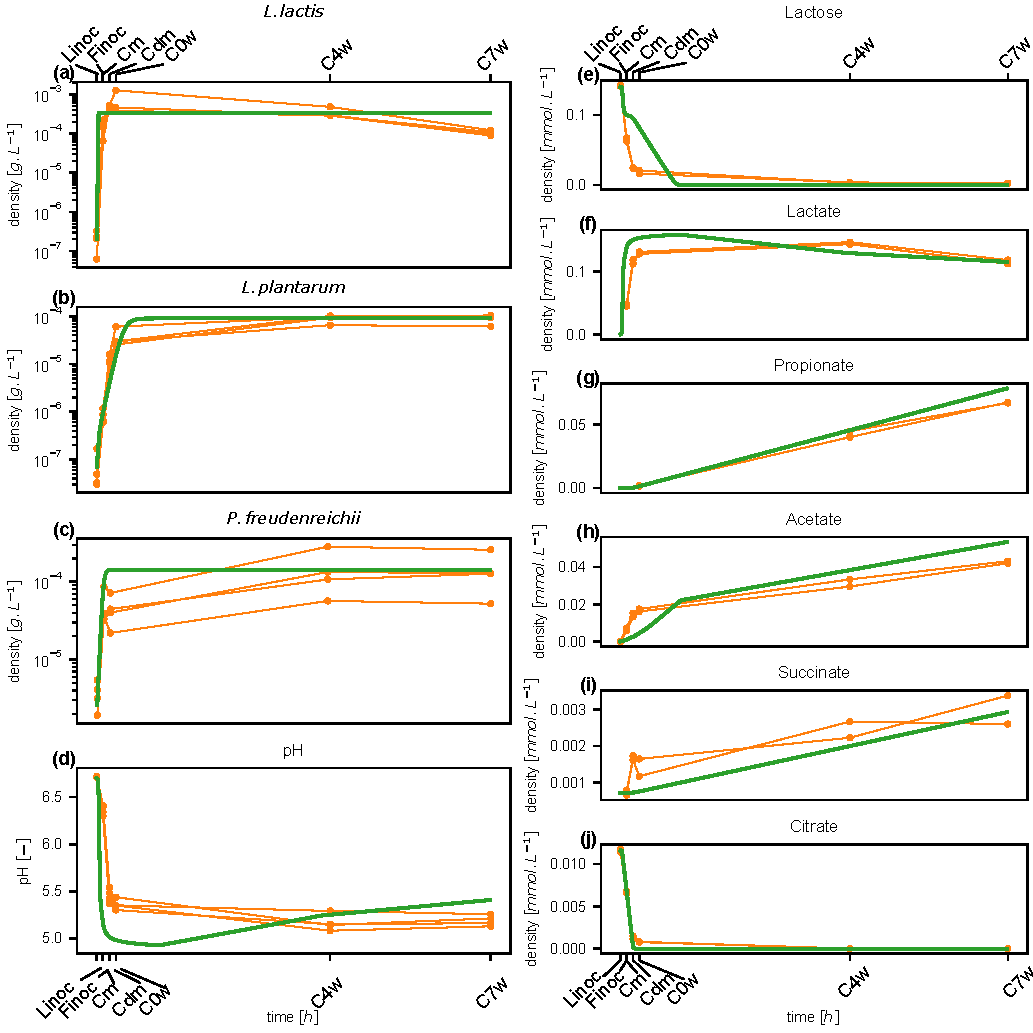
\includegraphics[width = 1.0\textwidth]{img/tango/Fig5.pdf}
    \caption{(a-c) Courbes de croissance de respectivement  \textit{L. lactis}, \textit{P. freudenreichii} and \textit{L. plantarum} calculées par le modèle (ligne verte) et celles observées expérimentalement (en orange). (d-j) Profil métabolique et du pH en condition de co-culture calculé par le modèle et expérimentalement observé. L'écart-type est représenté pour chaque point des données.  Abréviations: Linoc, innoculation des LAB (t = 0); Finoc, inoculation de \textit{P. freudenreichii}  (t = 18 hours); Cm, moulage (t = 19.5 hours); Cdm, démoulage (t = 40 hours); C0w, début d'affinage (t = 60 hours); C4w,4 semaines d'affinage (t = 732 hours); C7w, 7 semaines d'affinage (t = 1236 hours).}
    \label{dfba_community}
\end{figure}

\begin{figure}[H]
    \centering
    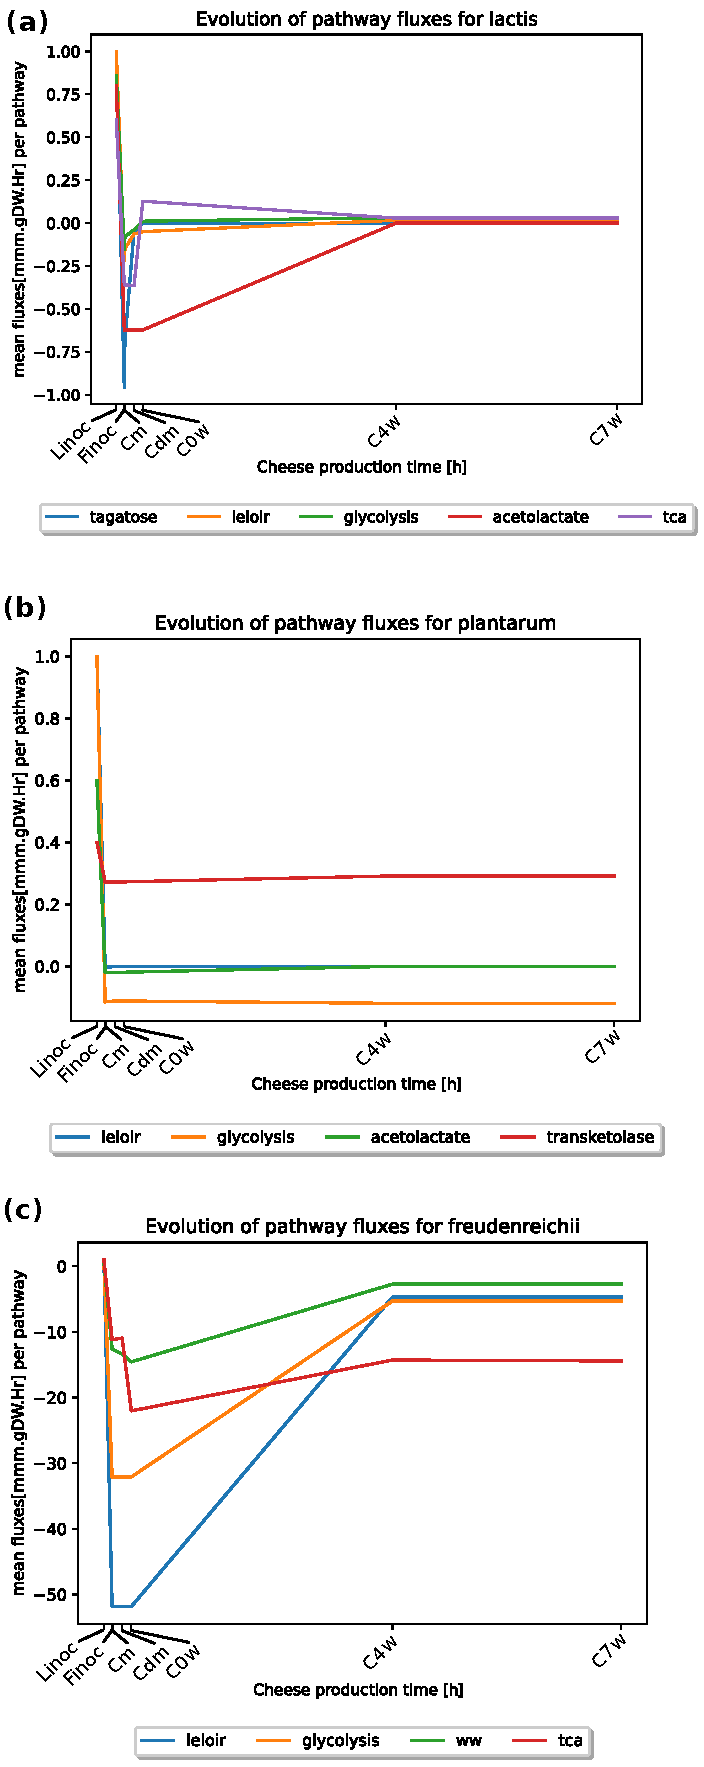
\includegraphics[width=0.5\textwidth]{img/tango/supp_fluxes_pathways.pdf}
    \caption{\textbf{Illustration du changement de voies métaboliques durant le processus de production du fromage.} Pour chaque bactérie nous avons lancé une simulation dynamique (dFBA) et les flux réactionnelles pour chaque voies métaboliques d'intérêt des figures \ref{figure:metabolic_map_lactis},\ref{figure:metabolic_map_plantarum},\ref{figure:metabolic_map_freud} on été retrouvé à l'incoculation de bactéries lactiques (Linoc, t=0 heure), de \freud (Finoc, t=18 heures), au moulage(t=19.5 heures), demoulage (Cdm, t=40heures), début de l'affinage (C0w, t=60 heures), après 4 (C4w, t=732 heures) et 7 (C7w, t=1236 heures) semaines d'affinage. Nous avons normalisés les flux par la valeur de flux lors de l'inoculum.}
    \label{fig:switch_metabolic_pathway}
\end{figure}

En somme, nous avons montré qu'utiliser uniquement des modèles métabolique curés et calibrés individuellement permet de retrouver les observations en communauté. Malgré les deux étapes itératives coûteuses en temps, l'interactivité entre modèle numérique et connaissance biologique \textit{a priori} permet d'obtenir des prédictions à l'échelle d'une communauté avec une bonne précision. Grâce à cette assurance, nous avons pu exploiter davantage le modèle de communauté du point de vue des interactions bactériennes possibles au sein de cette communauté. Dans les paragraphes suivant, nous déduirons dans un premier temps des interactions que notre approche numérique a pu mettre en évidence en analysant les flux relatifs et absolus de production et de consommation de métabolite par espèce. Dans un second temps, nous verrons ce que des outils sans connaissance \textit{a priori} peuvent découvrir.  \\

\subsection{Interactions bactériennes et exploration du modèle de communauté}

Notre modèle numérique de communauté peut révéler des interactions microbiennes du type syntrophiques, dans laquelle une espèce se nourrit des produits de l'autre, ou du type compétition pour un nutriment. Dans ce but, nous nous sommes focalisés sur la dynamique des flux des métabolites d'intérêt pour chaque espèce (Fig. \ref{fig:flux-contrib}, (a)) en calculant, à chaque pas de temps de la dynamique, et à l'échelle de la population, les flux d'échange $\mu_{i,j} b_i$ pour chaque métabolite $j$ et bactérie $i$ et les concentrations des métabolites associées. Concernant le lactose et le citrate, nous observons que \lactis les consomment très rapidement durant sa phase exponentielle Nous pouvons observer que \plantarum ne contribue pas ou peu à la consommation totale de ces métabolites suggérant ainsi que d'autres métabolites non suivis en dynamique sont utilisés pour la croissance de ce dernier, comme par exemple, les acides aminés. La croissance plus lente de \plantarum dans les premières heures du processus de production du fromage pourrait expliquer cette observation. En effet, on remarque que la régulation sur les bornes de consommation du lactose et du citrate sont mis en jeu lorsque la densité bactérienne de \plantarum est encore faible. De manière surprenante, nous observons que \freud termine la déplétion du lactose à la place de \plantarum au tout début de la phase d'affinage, bien que le lactate, source préférentielle de cette espèce, soit déjà produit, indiquant une ségrégation temporelle de l'utilisation de lactose, et une absence de compétition directe pour ce substrat.

\begin{figure}[H]  
    \centering
        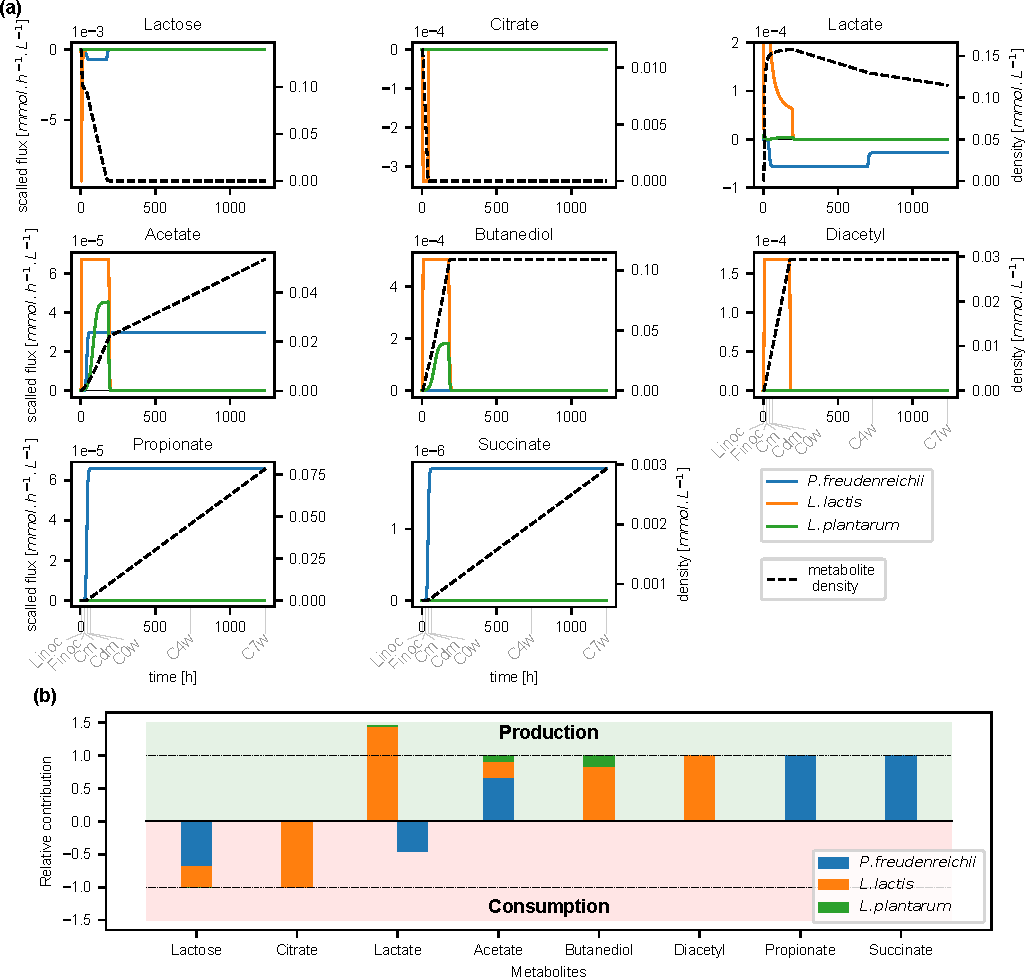
\includegraphics[width = 1.0\textwidth]{img/tango/Fig6.pdf}
        \caption{(a) \textbf{Flux dynamiques de consommation et de production de métabolites d'intérêts.} Nous representons pour chaque bactérie les flux dynamiques de consommation et de production de chaque métabolites que l'on en simulation (lignes coloriées). La dynamique de la concentration de ces mêmes métabolites dans le fromage est aussi représenté par les traits en pointillés. (b) \textbf{Contribution relative des bactéries dans le devenir des métabolites.} Nous avons calculé pour chaque souche sa contribution totale dans la consommation et la production de ces métabolites et intégré en temps par :$\int_0^t \mu_{i,j} b_i$ pour le métabolite $j$ et la bactérie $i$, voir eq.\ref{eq:system_dynamics_m}). Par la suite, nous avons normalisé le résultat par la somme des bactéries. La valeur 1 (resp. -1) représente la production (consommation) nette, \textit{i.e.}, la différence de concentration du métabolite à l'état final et initial (ligne en pointillé).  Abbreviations: Linoc, inoculation des bactéries lactiques (t = 0); Finoc, \textit{P. freudenreichii} inoculation (t = 18 hours); Cm, moulage (t = 19.5 hours); Cdm, Démoulage (t = 40 hours); C0w, début de l'affinage (t = 60 hours); C4w, 4 semaines d'affinage (t = 732 hours); C7w, 4 semaines d'affinage (t = 1236 hours).}
        \label{fig:flux-contrib}
    \end{figure}
    

La production de lactate étant corrélée avec la consommation de lactose, nous observons une très forte production par \lactis pendant 250 heures, correspondant à l'affinage dans le processus de fabrication du fromage. Malgré la plus faible croissance de \plantarum, ce dernier contribue peu à la production de lactate. Durant la phase de l'affinage, le lactate est consommé par \freud contribuant ainsi à l'augmentation du pH dans la communauté comme observé dans la Figure~\ref{dfba_community}~d. De façon surprenante, toutes les souches sont capables de produire l'acétate dans le milieu extracellulaire. \lactis est le contributeur majeur suivi par \plantarum jusqu'au temps t = 250 heures, temps à partir duquel la phase plateau commence. Ce schéma est retrouvé chez les bactéries lactiques intervenant également dans la production du butanediol \textit{via} la voie de l'acétolactate. Cependant, \freud continue de garder un taux de production constant d'acétate durant la maturation du fromage malgré la phase plateau atteinte. Enfin, le propionate et le succinate sont produits à taux constant par \freud durant tout le processus d'affinage et seule la souche de \lactis semble être capable de produire le diacétyle jusqu'au début de la période de l'affinage.\\

Afin d'obtenir la contribution en flux net de chaque souche au sein de ce consortium, nous avons intégré dans le temps la prédiction du FBA $\int_0^T \mu_{i,j}(t) b_i(t) dt$. Après normalisation de cet échange net par les échanges totaux au sein de la communauté (\textit{i.e.} la somme des échanges net de chaque individu), nous avons obtenu les contributions de chaque souche dans la production et la consommation de chaque métabolite (Fig. \ref{fig:flux-contrib}, (b)). Ces contributions confirment que le succinate et le propionate sont uniquement produits par \freud, alors que le diacétyle (production) et le citrate (consommation) sont métabolisés par \lactis. \plantarum contribue à la production du butanediol, bien que le principal producteur semble être \lactis. Dans une moindre mesure, \lactis contribue plus que \plantarum à la production de l'acétate dominée par \freud. En terme d'interactions bactériennes, on observe une syntrophie pour le lactate entre \lactis (producteur) et \freud (consommateur).\\

Nous avons démontré ci-dessus que capturer la complexité des processus métaboliques dans une communauté microbienne durant la fabrication de fromage requiert des considérations de la dynamique sous-jacente  du système. Nous nous demandions si l'application d'approches computationelles \textit{a priori} reposant sur les modèles métaboliques à l'échelle du génome peuvent mettre en avant de nouvelles interactions putatives entre les souches. A cette fin, nous avons utilisé deux méthodes basées sur les flux, SMETANA \citep{Zelezniak2015} et MiCOM \citep{diener2020}, et une approche qualitative basée sur le raisonnement, Metage2Metabo \citep{Belcour.2020} dans le but de suggérer de nouvelles complémentarités métaboliques au sein du consortium.

Les approches quantitative, MiCOM et SMETANA, ont mis en avant respectivement 14 et 25 métabolites échangés (Table\ref{table:exchangeable-metabolites-MICOM} et \ref{table:exchangeable-metabolites-smetana}), alors que l'approche par raisonnement, Metage2Metabo, identifie 11 métabolites qui ne peuvent pas être produits par une espèce sans interactions dans la communauté (Table \ref{table:added-value-M2M}). 

Une première observation est qu'un nombre assez important (11) de métabolites sont communs dans les prédictions des composés échangeables de SMETANA et MiCOM: lactate, qui est aussi prédit dans le modèle dynamique, phénylalanine, serine, malate, succinate, xanthine, H${_2}$S,2-ketoglutarate, glycolate et acetaldehyde. Les autres composés échangés prédits incluent principalement des acides aminés (isoleucine, proline, glycine, alanine). Pour chaque composé mis en avant par SMETANA nous avons utilisé les données méta-transcriptomiques dans le but d'évaluer la validité des interactions les plus plausibles selon le score SMETANA. Le H${_2}$S est prédit comme produit de \lactis et \plantarum au bénéfice de \freud, le ribose est produit par \lactis et \plantarum et consommé par \freud, le glycerol produit par les bacteries lactiques et consommé par \freud) et enfin la phénylalanine produite uniquement par \plantarum et consommée par \freud. Pour chacun de ces métabolites prédits comme échangés, nous avons vérifié l'expression des gènes associés à la production de ces métabolites chez les espèces donneuses, et à la consommation de ces métabolites chez les espèces receveuses (voir methodes et Figure \ref{fig:heatmap_metaT}). Les résultats suggèrent que les interactions pour H${_2}$S, ribose et le glycerol sont plausibles à plusieurs étapes de la fabrication du fromage. A l'inverse, alors que les données d'expression de gènes montrent que les voies métaboliques de la consommation de la phénylalanine sont fortement exprimées chez \freud, leur production par \plantarum ne l'est pas, suggérant que cette interaction semble être moins recevable. 


\begin{table}[H]
\centering
\begin{adjustbox}{width=\textwidth}
\begin{tabular}{|c|c|c|c|c|c|}
\hline
ID Bigg & ID Metacyc & Nom & Ontologie Metacyc&fluxes d'export & fluxes d'import\\
\hline
acald\_e	& ACETALD &	acetaldéhylde & Aldehydes-Or-Ketones, Aldehydes	& Pf; Ll &	Lp \\
akg\_e &	2-KETOGLUTARATE	& 2-oxoglutarate &	Acids, Organic-Acids	& Pf &	Lp \\
ala\_\_D\_e &	D-ALANINE &	D-ALANINE &	All-Amino-Acids, Acids, Amino-Acids, Organic-Acids	& Pf; Lp &	Ll \\
ala\_\_L\_e	& L-ALPHA-ALANINE &	L-ALPHA-ALANINE &	All-Amino-Acids, Acids, Amino-Acids, Organic-Acids	& Pf; Lp	& Ll \\
co2\_e &	CARBON-DIOXIDE	& CARBON-DIOXIDE	& Others, Others	& Pf; Ll &	Lp \\
coa\_e &	CO-A &	co enzyme A &	Groups, Others	& Pf; Ll	& Lp \\
fe2\_e	& FE+2	& Fe2+&	Ions, Inorganic-Ions, Cations &	Lp	& Pf; Ll \\
gly\_e	& GLY	& Glycine	& All-Amino-Acids, Acids, Amino-Acids, Organic-Acids &	Lp &	Pf; Ll \\
glyclt\_e &	GLYCOLATE &	GLYCOLATE	& Acids, Organic-Acids	& Pf &	Lp \\
gthox\_e &	OXIDIZED-GLUTATHIONE &	glutathione disulfide	& ORGANOSULFUR, All-Glutathiones &	Lp &	Ll \\
gthrd\_e	& GLUTATHIONE &	glutathione	& ORGANOSULFUR, All-Glutathiones, Thiols	& Ll	& Lp \\
h2o2\_e &	HYDROGEN-PEROXIDE &	hydrogen peroxide &	Peroxides, Others	& Ll &	Lp \\
h2o\_e	& WATER	& H2O	& Pseudo-Compounds, Others &	Pf; Ll	& Lp \\
h2s\_e	& HS	& hydrogen sulfide &	Ions, Anions, Inorganic-Ions	& Ll	& Lp; Pf \\
ile\_\_L\_e &	ILE &	isoleucine &	All-Amino-Acids, Acids, Amino-Acids, Organic-Acids &	Lp	& Pf; Ll \\
lac\_\_D\_e &	D-LACTATE &	d-lactate &	Acids, Organic-Acids	& Pf &	Ll; Lp \\
lac\_\_L\_e &	L-LACTATE &	l-lactate &	Acids, Organic-Acids &	Ll	& Lp; Pf \\
mal\_\_L\_e &	MAL	& malate &	Acids, Organic-Acids	& Pf; Lp &	Ll \\
nh4\_e &	AMMONIUM &	ammonium &	Ions, Inorganic-Ions, Cations	& Lp	& Pf; Ll \\
phe\_\_L\_e &	PHE &	phenylalanine &	Aromatics, All-Amino-Acids, Acids, Amino-Acids, Organic-Acids, Organic-aromatic-compounds &	Pf	& Lp \\
pro\_\_L\_e &	PRO &	proline &	All-Amino-Acids, Acids, Amino-Acids, Organic-Acids &	Ll	& Pf \\
ser\_\_D\_e &	D-SERINE &	serine	& All-Amino-Acids, Acids, Amino-Acids, Organic-Acids &	Ll	& Lp; Pf \\
ser\_\_L\_e &	SER	& serine &	All-Amino-Acids, Acids, Amino-Acids, Organic-Acids &	Ll &	Lp; Pf \\
succ\_e &	SUC	& succinate	& Acids, Organic-Acids &	Ll &	Pf \\
xan\_e &	XANTHINE &	xanthine &	Others, Others &	Ll	& Lp; Pf \\
 \hline
\end{tabular}
\end{adjustbox}
\caption{\textbf{Métabolites échangeable sur la communauté du fromage identifiés par MICOM} Abréviations: Ll, \lactis; Lp, \plantarum, Pf, \freud}
\label{table:exchangeable-metabolites-MICOM}
\end{table}

\begin{table}[H]
\centering
\begin{adjustbox}{width=\textwidth}
\begin{tabular}{|c|c|c|c|c|c|}
\hline
ID Bigg & ID Metacyc & Nom & Ontologie Metacyc &fluxes d'export & fluxes d'import\\
\hline
acald\_e	& ACETALD	& acetaldéhylde	& Aldehydes-Or-Ketones, Aldehydes & \multicolumn{1}{c|}{{\begin{tabular}[c]{@{}l@{}}Pf \\ Pf \\ Lp \\ Ll \end{tabular}}}
& \multicolumn{1}{c|}{{\begin{tabular}[c]{@{}l@{}}Ll \\ Lp \\ Ll \\ Lp \end{tabular}}} \\
\hline
akg\_e &	2-KETOGLUTARATE	& 2-oxoglutarate &	Acids, Organic-Acids &\multicolumn{1}{c|}{{\begin{tabular}[c]{@{}l@{}} Lp \\ Pf  \end{tabular}}}
& \multicolumn{1}{c|}{{\begin{tabular}[c]{@{}l@{}} Pf \\ Lp \end{tabular}}} \\
\hline
fum\_e &	FUM	& fumarate &	Acids, Organic-Acids &\multicolumn{1}{c|}{{\begin{tabular}[c]{@{}l@{}}Pf \end{tabular}}}
& \multicolumn{1}{c|}{{\begin{tabular}[c]{@{}l@{}}Lp \end{tabular}}} \\
\hline
glyc\_e &	GLYCEROL &	GLYCEROL &	Alcohols, All-Carbohydrates, Sugar-alcohols, Carbohydrates &\multicolumn{1}{c|}{{\begin{tabular}[c]{@{}l@{}}Lp \\ Ll \\ Ll \end{tabular}}}
& \multicolumn{1}{c|}{{\begin{tabular}[c]{@{}l@{}}Pf \\ Pf \\ Lp \end{tabular}}} \\
\hline
glyclt\_e &	GLYCOLATE &	GLYCOLATE &	Acids, Organic-Acids &\multicolumn{1}{c|}{{\begin{tabular}[c]{@{}l@{}} Lp \end{tabular}}}
& \multicolumn{1}{c|}{{\begin{tabular}[c]{@{}l@{}} Pf \end{tabular}}} \\
\hline
h2s\_e	& HS	& hydrogen sulfide &	Ions, Anions, Inorganic-Ions &\multicolumn{1}{c|}{{\begin{tabular}[c|]{@{}l@{}}Lp \\ Pf \\ Ll \end{tabular}}}
& \multicolumn{1}{c|}{{\begin{tabular}[c]{@{}l@{}}Pf \\ Lp \\ Lp \end{tabular}}} \\
\hline
lac\_\_D\_e &	D-LACTATE	& d-lactate &	Acids, Organic-Acids &\multicolumn{1}{c|}{{\begin{tabular}[c]{@{}l@{}}Pf \\ Ll \end{tabular}}}
& \multicolumn{1}{c|}{{\begin{tabular}[c]{@{}l@{}}Lp \\ Lp \end{tabular}}} \\
\hline
lac\_\_L\_e &	L-LACTATE &	l-lactate &	Acids, Organic-Acids &\multicolumn{1}{c|}{{\begin{tabular}[c]{@{}l@{}} Ll \end{tabular}}}
& \multicolumn{1}{c|}{{\begin{tabular}[c]{@{}l@{}}Lp \end{tabular}}} \\
\hline
mal\_\_L\_e &	MAL	& malate &	Acids, Organic-Acids &\multicolumn{1}{c|}{{\begin{tabular}[c]{@{}l@{}}Pf \\ Lp \\ Pf \\ Ll \end{tabular}}}
& \multicolumn{1}{c|}{{\begin{tabular}[c]{@{}l@{}} Ll \\ Ll \\ Lp \\ Lp \end{tabular}}} \\
\hline
phe\_\_L\_e &	PHE	& phenylalanine &	\multicolumn{1}{c|}{{\begin{tabular}[c]{@{}l@{}} Aromatics, All-Amino-Acids, Acids, Amino-Acids \\Organic-Acids, Organic-aromatic-compounds \end{tabular}}}   &\multicolumn{1}{c|}{{\begin{tabular}[c]{@{}l@{}}Lp  \end{tabular}}}
& \multicolumn{1}{c|}{{\begin{tabular}[c]{@{}l@{}}Pf \end{tabular}}} \\
\hline
rib\_\_D\_e &	D-Ribopyranose &	D-Ribopyranose &	Aldehydes-Or-Ketones, All-Carbohydrates, Aldehydes, Carbohydrates &\multicolumn{1}{c|}{{\begin{tabular}[c]{@{}l@{}}Ll \\ Lp \\ Pf \\ Ll \end{tabular}}}
& \multicolumn{1}{c|}{{\begin{tabular}[c]{@{}l@{}}Pf \\ Pf \\ Lp \\ Lp \end{tabular}}} \\
\hline
ser\_\_D\_e	& D-SERINE	& serine &	All-Amino-Acids, Acids, Amino-Acids, Organic-Acids &\multicolumn{1}{c|}{{\begin{tabular}[c]{@{}l@{}}Ll \\ Lp
 \\ Pf \\ Lp \\ Pf \\ Ll\end{tabular}}}
& \multicolumn{1}{c|}{{\begin{tabular}[c]{@{}l@{}} Pf \\ Pf \\ Ll \\ Ll \\ Lp \\ Lp \end{tabular}}} \\
\hline
succ\_e &	SUC &	succinate &	Acids, Organic-Acids &\multicolumn{1}{c|}{{\begin{tabular}[c]{@{}l@{}}Ll \\ Lp \end{tabular}}}
& \multicolumn{1}{c|}{{\begin{tabular}[c]{@{}l@{}}Pf \\ Pf   \end{tabular}}} \\
\hline
xan\_e &	XANTHINE &	xanthine &	Others, Others &\multicolumn{1}{c|}{{\begin{tabular}[c]{@{}l@{}}Ll \\ Lp \end{tabular}}}
& \multicolumn{1}{c|}{{\begin{tabular}[c]{@{}l@{}}Pf \\ Pf   \end{tabular}}} \\
\hline
\end{tabular}
\end{adjustbox}
\caption{\textbf{Métabolites échangeable sur la communauté du fromage identifiés par SMETANA.} Abréviations: Ll, \lactis; Lp, \plantarum, Pf, \freud}
\label{table:exchangeable-metabolites-smetana}
\end{table}

\begin{figure}[H]
    \centering
    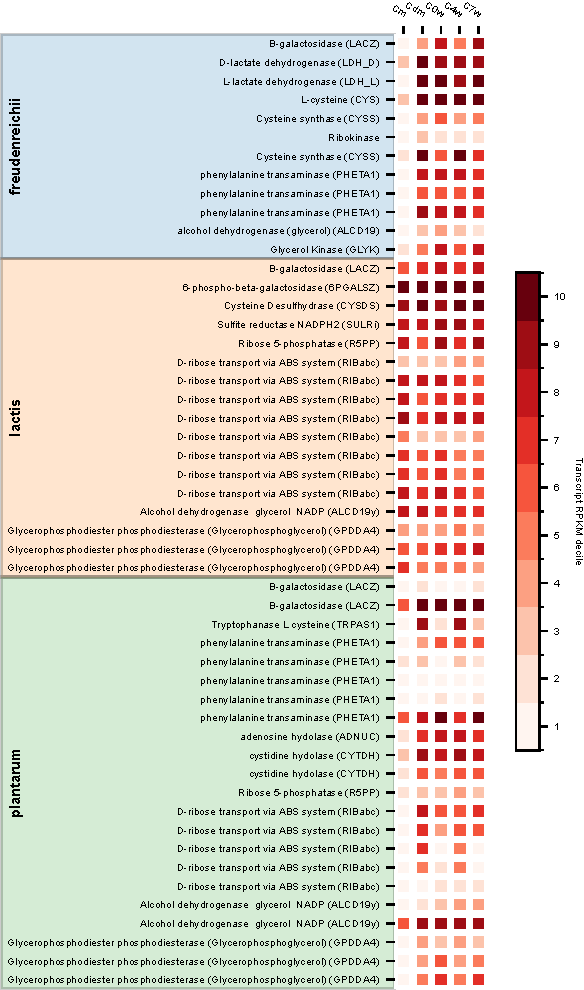
\includegraphics[width = 0.6\textwidth]{img/tango/FigS2_heatmap.pdf}
    \caption{\textbf{Expression des genes des données métatranscriptomiques} Cette carte thermique affiche le décile du nombre de RPKM de transcrits de gènes à un moment donné (colonnes) et dans un micro-organisme donné (les zones colorées indiquent à quelle bactérie le gène appartient). Les déciles ont ensuite été codés par couleur, des déciles les plus élevés (rouge foncé, expression la plus élevée dans ce micro-organisme à ce moment précis) aux déciles les plus bas (rouge clair, faible expression). Les gènes affichés ont été sélectionnés manuellement à partir de la liste des interactions possibles établie par SMETANA : pour un métabolite d'interaction sélectionné, les gènes impliqués dans la production (chez le donneur) et dans la consommation (chez le receveur) ont été retenus pour l'analyse. Les métabolites d'interaction sélectionnés sont le $H2S$, le ribose et la phénylalanine. En outre, les gènes impliqués dans la consommation de lactose ont été ajoutés à cette liste. Abbréviations: Cm, moulage (t = 19.5 hours); Cdm, démoulage (t = 40 hours); C0w, début de l'affinage (t = 60 hours); C4w, 4 semaines d'affinage (t = 732 hours); C7w, 7 semaines d'affinage (t = 1236 hours). }
    \label{fig:heatmap_metaT}
\end{figure}

Enfin, l'ensemble des métabolites dont la production est prédite par Metage2Metabo comme nécessitant des interactions dans la communauté inclut divers acides gras, comme le benzyl-Coa, le glyceraldehyde et la xanthosine, indiquant une complementarité métabolique entre les souches.



\begin{table}[H]
\centering
\begin{adjustbox}{width=\textwidth}
\begin{tabular}{|c|c|c|c|}
\hline
ID Bigg & ID Metacyc & Nom & Ontologie Metacyc  \\
\hline
galt1p&	D-galactose-1-phosphate&	a D-galactopyranose 1-phosphate	&All-Carbohydrates,Carbohydrates\\
benzcoa&	BENZOYLCOA&	benzoyl-CoA&	Esters,Thioesters\\
xtsn&	XANTHOSINE&	XANTHOSINE	&\begin{minipage}[t]{0.8\linewidth}Organic-heterocyclic-compound,All-Nucleosides,Nitrogen-Molecular-Entities,Organic-heteromonocyclic-compounds,Organic-Heteropolycyclic-Compounds,Organonitrogen-Compounds,Nucleosides\end{minipage}\\
glyald&	GLYCERALD&	glyceraldehyde	&Aldehydes-Or-Ketones,All-Carbohydrates,Aldehydes,Carbohydrates\\
3hocoa&	ø	&	ø	&	ø\\
3hhdcoa	&CPD0-2232	&(S)-3-hydroxyhexadecanoyl-CoA	&Thioesters,Esters\\
3hdcoa&	CPD0-2244	&(S)-3-hydroxydecanoyl-CoA	&Thioesters,Esters\\
3odcoa&	CPD0-2123&	3-oxodecanoyl-CoA	&Thioesters,Esters\\
3hhcoa&	OH-HEXANOYL-COA	&(S)-3-hydroxyhexanoyl-CoA&	Thioesters,Esters\\
udcpp&	UNDECAPRENYL-P	&all-trans-undecaprenyl phosphate	&Lipids,Polyisoprenoids\\
3oocoa&	CPD0-2106&	3-oxooctanoyl-CoA	&Thioesters,Esters\\
 \hline
\end{tabular}
\end{adjustbox}
\caption{\textbf{Liste de métabolites prédits par Metage2Metabo comme étant productibles uniquement par coopération métabolique}}
\label{table:added-value-M2M}
\end{table}

\section{Discussion et Conclusion}

Nous avons fourni un modèle numérique du métabolisme bactérien décrivant du point de vue métabolique, le processus de fabrication de fromage. En utilisant les modèles métaboliques de trois souches bactériennes inoculées et des données omiques, nous avons reproduit, avec précision, les motifs de production de métabolites ainsi que la dynamique des populations bactériennes. En nous reposant sur les conditions expérimentales de cultures pures pour calibrer les modèles métaboliques individuels avec peu de paramètres pour chacun, limitant ainsi le sur apprentissage du modèle durant les simulations communautaires. Une originalité du modèle est sa capacité à prédire les dynamiques sur tout le procédé de fabrication du fromage (sept semaines). Notre travail a généré des hypothèses sur les voies métaboliques mises en jeu dans le lait, ainsi que la contribution de chaque souche bactérienne dans la consommation de nutriments et la productibilité de composé organoleptiques. \\

La connaissance des microbiologistes, de la littérature scientifique et des données multi-omiques étaient nécessaires pour accomplir des modèles métaboliques à l'échelle du génome et des simulations dynamiques de qualité. Le métabolisme carboné central des bactéries lactiques produit principalement l'acide lactique à partir de la dégradation du lactose \textit{via} les voies métaboliques de la glycolyse, du tagatose et de Leloir \citep{Widyastuti2014,VanRooijen1991,Kleerebezem2003}. Pour la première fois, l'utilisation du citrate et de la fermentation hétérolactique ont été observé dans le modèle curé de \plantarum en lait. La vérification de modèle métabolique individuel et de l'activation des différentes voies métaboliques décrites plus haut représentait ainsi une étape importante pour valider les modèles, permettant la reproduction d'activités enzymatiques observées dans \citep{Quatravaux2006,Carroll1999}. La bactérie propionique \freud convertit le lactose, et préférentiellement le lactate en propionate d'après \citep{Loux2015,Thierry2011,Borghei2021}. Nous avons ajouté l'enzyme propionyl-CoA:succinate Coa transferase (2.8.3.-) pour compléter le cycle de Wood-Werkman, et ainsi assurer la production de propionate.

Dans \citep{Ozcan.2020}, les paramètres individuels de calibration pour chaque nutriment du milieu de culture sont imposés dans le but d'expliquer la métabolomique à l'échelle de l'espèce, et de prédire les composés de la métabolomique à l'échelle de la communauté. De plus, une nouvelle étape d'optimisation à l'échelle de la communauté a été faite afin d'affiner leur prédiction. Nous avons implémenté un modèle FBA dynamique en se basant sur \citep{Mahadevan.2002}, qui a utilisé des paramètres de calibration spécifiques aux souche pour prédire la croissance, le pH et les concentrations métaboliques. Pour éviter le sur apprentissage du modèle, nous avons réduit le nombre de paramètres inférés pour chaque bactérie. Seulement deux paramètres ont été gardés pour la régulation du pH pour les bactéries lactiques et un paramètre se focalisant sur les croissances de \plantarum et \freud. Des calibrations additionnelles ont été menées pour \freud sans aucune optimisation mathématique supplémentaire, en calculant la valeur de la borne supérieure des métabolites dosés en monoculture. Ainsi, nos paramètres ne sont pas propres à chaque nutriment et nous n'avons effectué aucune optimisation à l'échelle de la communauté.\\

Le modèle de co-culture a donné des indices sur le comportement de la communauté pendant la fabrication du fromage et a suggéré temporellement la contribution de chaque espèce impliquée dans la production des composés organoleptiques. Il est montré que la production de propionate peut être attribuée uniquement à \freud, comme indiqué dans \citep{Cao2021}, et que le diacétyl semble être seulement produit par \lactis. D'après le modèle de communauté, le butanediol a été produit pendant l'étape du moulage et au début de l'affinage par à la fois, \lactis et \plantarum, comme observé dans les modèles de monocultures respectifs. L'acétate est produit précocement jusqu'au début de l'affinage par les 3 espèces, puis, \freud, responsable de la majeure partie de production de l'acétate, semble le produire à flux constant jusqu'à la fin de la fabrication de fromage. Concernant l'utilisation des sources de carbone, alors que \plantarum possède les voies métaboliques de dégradation du lactose et du citrate, qui sont complètement activées dans le modèle en monoculture, il apparaît que ces voies métaboliques sont fortement sous régulés en co-culture et \plantarum ne semble plus être capable de métaboliser le citrate. Lors de la mise en culture avec \lactis, \plantarum atteint son efficacité métabolique maximale après la phase exponentielle de \lactis comme ce dernier a la plus faible vitesse de croissance. Étant donné que \lactis pousse principalement sur le lactose en produisant du lactate, sa phase exponentielle est associée à une forte acidification de milieu, réprimant probablement le métabolisme de \plantarum (voir equation sur la régulation du pH sur les bactéries lactiques). \plantarum peut utiliser des acides aminés ou d'autres métabolites non suivis par le modèle dynamique permettant sa croissance. Pour explorer cette piste, nous avons utilisé des outils dans le but d'identifier des interactions bactériennes en dehors de l'ensemble des composés suivis par le modèle dynamique en co-culture. Nous avons remarqué que parmi les possibles interactions, la famille des acides aminés était bien représentée.\\

Dans le modèle de co-culture, \freud garde son métabolisme activé  dans la dernière phase de production d'un fromage : l'affinage. Ce métabolisme est reflété par la consommation de lactate durant tout l'affinage, et le relargage de composés organoleptiques à flux constant (Figure \ref{fig:flux-contrib}). Ce comportement est cohérent avec les capacités métaboliques connues de \freud et avec les données métabolomiques obtenues expérimentalement. Dans le modèle, \freud consomme aussi le lactose restant après la croissance de \lactis. En effet, durant sa phase exponentielle, \lactis métabolise principalement le lactose, produisant fortement du lactate et réduisant le pH. La réduction du pH inhibe l'absorption du lactose dans les deux bactéries lactiques, et donc stoppant la consommation de lactose par les \textit{Lactobacilli}. Comme le lactose reste dans le milieu de culture et que \freud est l'unique bactérie capable de l'utiliser, il épuise donc le lactose encore présent. Dans les données métatranscriptomiques, le gène LACZ est fortement activé par \freud durant l'affinage confirmant la dégradation du lactose par cette souche après l'acidification (Figure \ref{fig:heatmap_metaT}) 


Ce chapitre a révélé comment le processus itératif, la combinaison d'expertise biologique, de données hétérogènes et de la modélisation métabolique permet d'obtenir des prédictions précises sur les mécanismes responsables du comportement dynamique de la communauté microbienne. D'autre part, cela souligne également que la quantité de données et les efforts nécessaires pour créer des modèles de haute qualité restent un prix élevé à payer malgré l'amélioration des approches de simulation. Des développements méthodologiques doivent encore être proposés afin d'automatiser la calibration des modèles avec des données, et de garantir à la fois l'exactitude des prédictions et l'extensibilité à des 
communautés plus importantes ou à des communautés de composition empirique.\\


Dans le chapitre suivant, nous présentons une approche permettant l'analyse haut débit de communautés bactériennes en utilisant une approche discrète du métabolisme. Nous nous focaliserons sur la mise en évidence de potentiel de coopération et compétition dans des communautés synthétiques et réelles. Du point de vue général de la thèse, le chapitre sur la modélisation numérique et celui sur la modélisation discrète du métabolisme constituent respectivement le cas riche et le cas pauvre pour l'analyse du métabolisme. Un dernier chapitre se consacrera sur l'enrichissement de modèle logique pour se rapprocher du modèle numérique tout en conservant les propriétés de passage à l'échelle et d'explicabilité.
\newpage

\section*{Abréviations métaboliques}
\label{abbreviation-metabo}
\noindent
13dpg \hspace{.5em} 3-Phospho-D-glyceroyl phosphate \\
6pgc \hspace{.5em} 6-Phospho-D-gluconate \\
6pgl \hspace{.5em} 6-phospho-D-glucono-1,5-lactone \\
ac \hspace{.5em} acétate \\
acald \hspace{.5em}  acetaldehyde \\
accoa \hspace{.5em} acetyl-coa \\
actn\_\_R \hspace{.5em} acetoine  \\
akg \hspace{.5em}  2-Oxoglutarate \\
alac\_\_S \hspace{.5em} (S)-2-Acetolactate \\
btd\_RR \hspace{.5em}  butanediol \\
cit \hspace{.5em} citrate \\
dgal6p \hspace{.5em} d-galactose-6-phosphate \\
dhap \hspace{.5em} Dihydroxyacetone phosphate \\
diact \hspace{.5em} diacetyl \\
f6p\hspace{.5em} fructose-6-phosphate \\
fdp \hspace{.5em} D-Fructose 1,6-bisphosphate \\
fum \hspace{.5em} fumarate \\
g1p \hspace{.5em} glucose-1-phosphate \\
g3p \hspace{.5em} Glyceraldehyde 3-phosphate \\
g6p \hspace{.5em} glucose-6-phosphate \\
gal \hspace{.5em} galactose \\
gal1p \hspace{.5em} galactose-1-phosphate \\
 glc\_\_D \hspace{.5em} glucose\\
 lac\_\_D, lac\_\_L \hspace{.5em} citrate \\
lac6p \hspace{.5em} lactose-6-phosphate \\
lcts \hspace{.5em} lactose \\
mmcoa\_\_R \hspace{.5em} (R)-Methylmalonyl-CoA \\
mmcoa\_\_S \hspace{.5em} (S)-Methylmalonyl-CoA \\
oaa \hspace{.5em} Oxaloacetate \\
ppa \hspace{.5em} propionate \\
ppap \hspace{.5em} Propanoyl phosphate \\
ppcoa \hspace{.5em} propionyl-coa \\
pyr \hspace{.5em} pyruvate \\
ru5p\_\_D \hspace{.5em} D-Ribulose 5-phosphate \\
succ \hspace{.5em} succinate \\
succoa \hspace{.5em} succinyl-coa \\
tag6p\_\_D \hspace{.5em} D-tagatose-6-phosphate \\
tagdp\_\_D \hspace{.5em} D-Tagatose 1,6-biphosphate \\
udpg \hspace{.5em} UDPglucose \\
xu5p\_\_D \hspace{.5em} D-Xylulose 5-phosphate \\

\newpage
\section*{Abréviations réactionnelles}
\label{abbreviation-reac}
\noindent
2131pyrpp \hspace{.5em} Methylmalonyl-CoA carboxyltransferase 5S subunit \\
6PGALSZ \hspace{.5em} 6-phospho-beta-galactosidase \\
ACLD \hspace{.5em} Acetolactate decarboxylase \\
ACTD2 \hspace{.5em} Acetoin dehydrogenase \\
ACLDC \hspace{.5em} Acetolactate decarboxylase \\
ACLS \hspace{.5em} Acetolactate synthase \\
BTDD\_RR \hspace{.5em} R R  butanediol dehydrogenase \\
CITL \hspace{.5em} Citrate lyase \\
CITt4\_1 \hspace{.5em} Citrate transport via sodium symport \\
CS \hspace{.5em} Citrate synthase \\
D\_LACt2 \hspace{.5em} D lactate transport via proton symport \\
ENO \hspace{.5em} Enolase \\
FBA \hspace{.5em} Fructose-bisphosphate aldolase \\
FEDCabc \hspace{.5em} FEDCabc \\
FRD2rpp \hspace{.5em} Fumarate reductase/succinate dehydrogenase \\
G6PDH2r \hspace{.5em} Glucose 6-phosphate dehydrogenase \\
GAL6PI \hspace{.5em} Galactose-6-phosphate isomerase \\
GALkr \hspace{.5em} Galactokinase \\
GALUi \hspace{.5em} UTP-glucose-1-phosphate uridylyltransferase (irreversible) \\
GAPD \hspace{.5em} Glyceraldehyde-3-phosphate dehydrogenase \\ 
GND \hspace{.5em} Phosphogluconate dehydrogenase \\
HEX1 \hspace{.5em} Hexokinase (D-glucose:ATP) \\
L\_LACt2r \hspace{.5em} L lactate reversible transport via proton symport \\
LACpts \hspace{.5em}  Lactose transport via PEP:Pyr PTS \\
LACZ \hspace{.5em} B-galactosidase \\
LCTSt3ipp \hspace{.5em} Lactose transport via proton aniport (periplasm) \\
LDH\_D \hspace{.5em} D-lactate dehydrogenase; \\
LDH\_L \hspace{.5em} L-lactate dehydrogenase \\
MME \hspace{.5em} Methylmalonyl-CoA epimerase \\
MMM2 \hspace{.5em} Methylmalonyl-CoA mutase \\
OOR3r \hspace{.5em} 2-oxoglutarate synthase (rev) \\
PC \hspace{.5em} Pyruvate carboxylase \\
PFK\_2 \hspace{.5em} Phosphofructokinase \\
PFL \hspace{.5em} Pyruvate formate lyase; \\
PGI \hspace{.5em} Glucose-6-phosphate isomerase \\
PGK \hspace{.5em} Phosphoglycerate kinase \\
PGL \hspace{.5em} 6-phosphogluconolactonase \\
PGM \hspace{.5em} Phosphoglycerate mutase \\
PGMT \hspace{.5em} Phosphoglucomutase \\
phosphoketolase \hspace{.5em} phosphoketolase \\
PPAKr \hspace{.5em} Propionate kinase \\
PPCSCT \hspace{.5em} Propanoyl-CoA: succinate CoA-transferase \\
PTA \hspace{.5em} Phosphotransacetylase \\
PTA2 \hspace{.5em} Phosphate acetyltransferase \\
PYK \hspace{.5em} Pyruvate kinase \\
RPE \hspace{.5em} Ribulose 5-phosphate 3-epimerase \\
TGBPA \hspace{.5em} Tagatose-bisphosphate aldolase \\
UGLT \hspace{.5em} UDPglucose--hexose-1-phosphate uridylyltransferase \\


% \ifdefined\FromMain %
% \else % 
\end{document} %

% \newpage
%
%\subfile{chapitres/cocomico_v2.tex}
%% \documentclass[../main.tex]{subfiles}

\begin{document}

\chapter{Modèle discret pour le criblage haut-débit du potentiel d'interaction métabolique dans les écosystèmes microbiens complexes}
\label{ccmc}
\minitoc
Article en cours de rédaction 
%\textit{journal theory of biology}. \footnote{\url{https://www.sciencedirect.com/journal/journal-of-theoretical-biology}}

%\doublespacing %% For correction

\newpage

\section{Introduction}
Dans le chapitre précédent, nous avons développé une approche itérative permettant de prédire des concentrations de métabolites, la densité bactérienne ainsi que quelques interactions bactériennes dans un écosystème composé de 3 souches bactériennes. Cette approche est numériquement trop coûteuse en temps pour permettre une analyse haut-débit d'écosystèmes microbiens plus complexes. De plus, la prédiction des interactions bactériennes a été faite avec confiance grâce à la connaissance \textit{a priori} des biologistes, de la littérature et des données expérimentales. Dans le cadre d'un écosystème naturel, appliquer le processus itératif décrit dans le chapitre \ref{tango} est compromis par le manque de la connaissances \textit{a priori} du système. En effet, raffiner des modèles métaboliques appartenant à des organismes peu étudiés et générer des données de calibration pour des communautés composées de centaines d'espèces sont irréalisables. \\

La stabilité des communautés microbiennes se reposent en partie sur les interactions bactérie-bactérie, principalement caractérisées par la consommation et la production de métabolites. Ces interactions sont particulièrement importantes car elles sont responsables du fonctionnement du microbiome: protection de l'hôte dans le microbiote de l'intestin \citep{WILMES20221201}, recyclage de matières organique dans le sol \citep{Rousk2016}, participation à la croissance de la plante \citep{FOURNIER202227} ou encore, ou développement d'arôme dans la fermentation du fromage \citep{Cao2021}. Pour rappel, il existe plusieurs types d'interaction comme illustré par la Figure \ref{fig:interaction}. La coopération est déterminée comme un échange métabolique positif, sans effet négatif pour la bactérie productrice et la receveuse. A l'opposé, la compétition est décrite comme un coe-consommation d'un substrat limitant impactant la croissance et /ou la production métabolique des bactéries en compétition.\\

Dans la littérature, nous avons observé que les méthodes pour identifier des potentiels de coopération et de compétition dans des communautés de grande taille s'intéressaient à l'étude du métabolisme (voir chapitre \ref{ch:edla}). En effet, en utilisant la relation d'association gène-protéine-réaction d'un réseau métabolique à l'échelle du génome (GEM), une représentation sous forme d'une matrice st\oe{}chiométrique, d'un graphe ou à l'aide d'approches de raisonnement peuvent être utilisé pour mettre en avant ces interactions. Comme nous l'avons vu, les approches numériques sont principalement limitées par le coût calculatoire. Les approches basées sur les graphes ne sont pas non plus adaptées à la caractérisation de ces potentiels d'interactions lorsque que le nombre d'organisme dans la communauté est important. En effet, des approches se basent sur des analyses par paire d'organismes, rendant fastidieuse l'analyse à l'échelle de la communauté. Il existe cependant un compromis, permettant de caractériser la communauté dans son ensemble, comme les méthodes numériques, et permettant de passer à l'échelle de grandes communautés: \textbf{l'approche par raisonnement} \citep{Belcour.2020, Frioux2018}. Au moyen d'un formalisme logique, des règles décrivant la notion de productibilité d'un composé sont décrites (voir chapitre \ref{EDLA}). \\

Pour caractériser les potentiels d'interactions à l'aide de l'approche par raisonnement, une base de connaissance décrivant l'objet d'étude sous forme d'une liste de faits biologiques doit être créée. Dans notre cas, elle est constituée des attributs d'un réseau métabolique que sont: produit, réactant, réaction, métabolite. Cette base de connaissance va permettre d'analyser rapidement la productibilité des composés, la faisabilité des réactions ou encore, d'identifier les échanges métaboliques etc. Toutes ces propriétés émergeantes sont calculables à partir d'une liste de règles inspirées des définitions biologiques décrivant ces mêmes particularités. Ainsi, chaque modèle en sortie découlera explicitement de la règle biologique auditable. Le paradigme de programmation par ensemble de réponse (de l’\textit{anglais, Answer set Programming} ou ASP) a été choisi pour ses qualités: explicabilité des modèles et résolution des problèmes combinatoires.\\

Dans ce chapitre, nous avons donc utilisé la programmation par ensemble de réponse (ASP) et s'inspiré de l'algorithme d'expansion du réseau métabolique d'Ebenhoh \citep{Ebenhoh2004} et de son élargissement à la caractérisation de communauté \citep{Frioux2018} en créant une nouvelle base de connaissance à partir d'un ensemble de GEMs. De cette base de faits, des nouvelles règles logiques sont créées permettant le calcul d'un potentiel de coopération et de compétition. Dans la suite, nous présenterons la nouvelle base de connaissance et les règles logiques que nous avons développées, puis une série de tests montrant la pertinence des scores de coopération et de compétition. Enfin, une comparaison à des méthodes quantitatives sera effectuée. \\

Les travaux présentés dans ce chapitre ont mené à un article en cours de rédaction et à plusieurs posters scientifiques et présentations orales \citep{lecomte:hal-03839337,lecomte:hal-03857781, lecomte:hal-03857848}

%pour une soumission dans \textit{journal of theory biology} \footnote{\url{https://www.sciencedirect.com/journal/journal-of-theoretical-biology}}

\newpage
\section{Méthode pour calculer un score d'interaction à partir d'une base de connaissance}
Le choix de la représentation de la connaissance est primordial pour toute approche par raisonnement. Nous détaillerons dans un premier temps, comment nous avons représenté mathématiquement et en ASP la base de faits, ainsi que les règles logiques pour inférer les potentiels d'interaction.

\subsection{Base de faits d’un réseau métabolique}
À partir de la donnée d'entrée, un GEM, nous avons défini des ensembles de réactions \Rs, métabolites \Ms et de taxa \Ts où taxon représente l'identifiant du GEM. Nous avons associé chaque ensemble de métabolites \Ms et réactions \Rs à son taxon \Ts et récupéré le nom ontologique donné dans le GEM $\name$ comme suit:

\begin{align}
	\begin{split}
		& \source: \Ms \rightarrow \Ts \\
		& \source: \Rs \rightarrow \Ts \\
		& \name: \Ms \rightarrow \mbox{\textit{identifiant}}
	\end{split} 
\end{align}

L'association d'un métabolite ou d'une réaction à son taxon permet d'obtenir la réaction ou le métabolite à partir d'un ensemble de taxa:

\[\projection{t\in\Ts} = \{ m \in M \suchthat \source(m) = t \}\]

Nous avons par la suite défini les relations entre les métabolites, réactions et taxon sous la représentation d'un graphe bipartite. Pour rappel, une réaction est composée d'un ensemble de réactant et de produit, et nous le formalisons de la façon suivante:

\begin{align}
\begin{split}
    \products(\gmodel) &= \{ m\in M \suchthat \langle r, m\rangle \in E \} \\
    \reactants(\gmodel) &= \{ m\in M \suchthat \langle m, r\rangle \in E \} \\
    \taxons(M) & = \{ t \in T \suchthat \exists m\in M ,\, \source(m) = t \}
\end{split}
\end{align}

dans lequel, \gmodel est le tuple défini par $\langle M, R, E \rangle$, $r \in \Rs$; où chaque arc $e = \langle m,r \rangle$ encode un \emph{réactant} consommé par la réaction $r$ et $e = \langle r,m \rangle$ encode un \emph{produit} produit de $r$. \\

Tout comme pour le modèle numérique, un choix concernant la prise en compte des réactions de transport présentes dans le réseau métabolique a été fait. Il a été montré que le phénomène de lyse cellulaire était une potentielle source d'interaction métabolique, entrainant la mort de la cellule et libérant son contenu métabolique dans le milieu extracellulaire \citep{Fazzino2020}. De plus, \citep{Pacheco.2019m3q} ont montré que les sécrétions passives étaient une source de mutualisme au sein de communautés bactériennes. De ce fait, lors de la conception du modèle de communauté, nous avons choisi de considérer les ensembles de métabolites produits en intracellulaire disponibles pour tous. Ainsi, un modèle de Communauté \( \gcommunity = \{ \gmodel[1], ..., \gmodel[n] \}\) peut-être décrit comme le produit cartésien de l'union des métabolites et réactions défini par le graphe bipartite, et se lit ainsi:

\[
\merge(\gcommunity) = 
\left\langle \bigcup^{n}_{i=1} M_i, \bigcup^{n}_{i=1} R_i, \bigcup^{n}_{i=1} E_i \right\rangle \,.
\]

\subsection{Productibilité d'un métabolite}
Pour rappel, un métabolite $mp$ est productible si l'ensemble des réactants d'une réaction, permettant la production de ce métabolite $mp$, sont disponibles à partir d'un ensemble de graines, constitué de l'ensemble des composés du milieu nutritif. Dans la suite de ce chapitre, nous qualifierons de \emph{scope} l'ensemble des métabolites productibles par un réseau à partir de graines. Du fait de notre représentation de la base de connaissance, dans lequel chacun des métabolites et réactions est associé à un GEM, nous n'avons plus la nécessité de distinguer le \emph{scope} associé à un individu de celui de la communauté comme dans \citep{Frioux2018}. Ainsi, à partir d'un ensemble de graines $S$ et pour une communauté de GEMs $\gmodel$, le \emph{scope} est défini comme suit:

\[
\begin{split}
    \scope(\gcommunity,S) & = \bigcup^{\infty}_{i=0} \scope_i \mbox{, où} \\
    \scope_0 & = S\\
    \scope_{i+1} & = \scope_i \bigcup \products(\{ r \in R \suchthat \\ 
     & \name(\reactants(r)) \subseteq \name(\scope_i) \}) \,.
\end{split}
\]

Pour implémenter cette notion de productibilité et calculer des potentiels de coopération et de compétition, nous avons utilisé une approche par raisonnement.

\subsection{L'inférence des règles logiques pour calculer les potentiels de coopération et de compétition}
Cette sous-section présentera comment nous avons implémenté en ASP les définitions de \texttt{scope}, de coopération et de compétition.

\paragraph*{Inférence du scope métabolique.} 
A partir d'un objet métabolite, dans lequel un nom et un taxon sont associés, (\texttt{metabolite(M,B)}) et d'une communauté (\texttt{Communaute}), le \texttt{scope} métabolique d'une communauté est défini par le code \ref{lst:scope} et \ref{lst:disponible}. Dans la suite de cette section, chaque listing sera expliqué ligne par ligne sous forme d'item, afin de comprendre les règles logiques. 

\begin{lstlisting}[mathescape=True,label={lst:scope},caption={Code ASP permettant de calculer le scope métabolique}, captionpos=b]
scope(metabolite(M,B), Communaute) :- taxon(B);  
               in_community(Communaute,B); 
               reaction(R,B); product(M,R,B); 
               disponible(M', Communaute) : reactant(M',R,B).
\end{lstlisting}

Au sein du listing \ref{lst:scope}, un métabolite est dans le scope d'une communauté si :
\begin{itemize}
	\item[ligne 1:] le \texttt{scope} métabolique, d'une communauté est vrai si, \texttt{B} est un taxon et
	\item[ligne 2:] que \texttt{B} est un membre de la communauté et
	\item[ligne 3:] qu'il existe une réaction \texttt{R} du taxon \texttt{B} qui produit \texttt{M} et 
	\item[ligne 4:] que tous les métabolites réactants de la réactant \texttt{R} du taxon \texttt{B} sont disponibles pour la communauté.\\
\end{itemize}

De cette règle découle la notion de disponibilité d'un métabolite (voir listing \ref{lst:disponible})

\begin{lstlisting}[mathescape=True, label={lst:disponible}, caption={Code ASP permettant de savoir si un métabolite est disponible},captionpos=b]
disponible(M,Com) :- graine(M), Communaute(Com). 
disponible(M,Com) :- scope(metabolite(M,B), Com).
\end{lstlisting}

où :

\begin{itemize}
	\item[ligne 1:] Un métabolite \texttt{M} est disponible pour une communauté \texttt{Com} si le métabolite M est une graine et que \texttt{Com}  est une communauté de GEMs où
	\item[ligne 2:] que le métabolite \texttt{M} appartenant à un taxon \texttt{B} est dans le \texttt{scope} métabolique de la communauté \texttt{Com}. 
\end{itemize}

\paragraph*{Inférence des métabolites échangeable.} Nous avons pris le postulat que les métabolites échangés correspondent à l'approximation la plus directe de la coopération d'une communauté. Nous l'avons défini comme un métabolite qui est productible par un GEM, consommable par un autre et qui ne peut être produit par ce dernier:

\[
\begin{split}
\exchange_{\gcommunity, S}(\hat{m}) = \{ \langle P, C \rangle \suchthat &
         \exists \gmodel[C]\in\gcommunity,
         \exists \gmodel[P]\in\gcommunity, \\
    &    \exists m \in \reactants(\gmodel[C]), \\
    & \name(m) = \hat{m}, \\
    & m \in \products(\gmodel[P]), \\
    & m \not\in \scope(\gmodel[C],S), \\
    & m \in \projection{P}(\scope(\gcommunity, S)) \;\} \\
\end{split}
\]
dans lequel $S$ correspond au \texttt{scope} métabolique, $P$ et $C$ respectivement les taxa producteur et consommateur.

Le code ASP correspondant est similaire à sa représentation mathématique et est défini par le code \ref{lst:echange}:
\begin{lstlisting}[mathescape=True, label={lst:echange}, caption={Code ASP permettant d'obtenir l'ensemble des métabolites qui sont potentiellement échangés.}, captionpos=b]
exchange(M,P,C) :- taxon(P), 
		 taxon(C),
		 P != C,
		 reactant(M,_,C),
		 product(M,_,P),
		 scope(metabolite(M,P), all),
		 not scope(metabolite(M,C), self(C)).
\end{lstlisting}

où:

\begin{itemize}
	\item[ligne 1:] un métabolite \texttt{M} est échangeable entre un producteur \texttt{P} et un consommateur \texttt{C} si \texttt{P} est un taxon et 
	\item[ligne 2:] que \texttt{C} est un taxon et
	\item[ligne 3:] \texttt{P} est différent de \texttt{C} et
	\item[ligne 4:] que \texttt{M} est un réactant de n'importe quelle réaction de \texttt{C} et 
	\item[ligne 5:] que \texttt{M} est un produit de n'importe quelle réaction de \texttt{P} et
	\item[ligne 6:] que \texttt{M} est dans le \texttt{scope} communautaire et 
	\item[ligne 7:] que \texttt{M} n'est pas dans le \texttt{scope} de \texttt{C}.
\end{itemize}

Nous avons décrit le \texttt{scope} métabolique pour un GEM ou une communauté de GEMs, et identifié les métabolites échangeables comme un proxy de la coopération. Concernant la compétition, la notion de substrat limitant est reliée à la quantité de ressource de ce substrat  disponible pour la communauté. Ce formalisme discret ne permet actuellement pas de prendre la notion de quantité, nous nous sommes inspirés d'un concept d'économie pour définir une compétition: polyopsonie. D'origine grec, l'éthymologie de monopsone appliqué à l'économie signifie un marché dans lequel il y a un seul acheteur (\textit{mono} signifie un, et \textit{opsonia}  signifie achat). Un marché où il existe un petit nombre d'acheteur est charactérisé par l'oligopsone. En s'inspirant des deux concepts economiques ci-dessus, nous avons élaboré un nouveau mot représentant un marché où il existe plusieurs acheteurs: polyopsone.


\paragraph*{Inférence de la polyopsonie.} Ainsi, la polyopsonie reflète une approximation de la compétition et stipule que les substrats limitants, \textit{i.e.} métabolites échangeables et ceux qui sont consommés par plus d'un organisme, sont considérés comme substrats en compétition. Mathématiquement, cela se traduit par:

\begin{align}
	\begin{split}
	\lims(\gcommunity,& S) = \{ \name(m) \suchthat
     	\exists m\in \reactants(\scope(\gcommunity, S)), \\
    	& \vert \taxons(m) \vert > 1 \;\wedge \\
    	& (\name(m) \in S \vee 
      	\exchange_{\gcommunity,S}(\name(m)) \neq\emptyset) \;\} \, . \\
	\end{split}
\end{align}
dans lequel $m$ est un métabolite. \\
%
%
%Littéralement, cette expression signifie que pour chaque métabolite $m$ considéré comme réactant dans le scope ($m\in \reactants(\scope(\gcommunity, S))$) et est consommé par au moins 2 individus ($\vert \taxons(m) \vert > 1$) et qu'il est échangeable ($\exchange_{\gcommunity,S}(\name(m)) \neq\emptyset) \;\} $) alors, nous le considérons comme limitant. \\

Dans le code mathématique ci-dessus, le facteur déterminant un substrat limitant concerne le nombre de taxa consommant un métabolite. Ainsi, dans le code ASP permettant d'obtenir les substrats qui sont limitants (voir listing \ref{lst:competition}), nous avons compté le nombre de taxa consommant chaque substrat, échangé ou considéré comme un nutriment, et appliqué la condition du nombre de consommateur:

\begin{lstlisting}[mathescape=True,label={lst:competition}, caption={Code ASP permettant d'obtenir l'ensemble des consommateurs en compétition pour un substrat limitant.}, captionpos=b]
% cas pour les metabolites echangeables
polyopsonist(M,N) :- N=#count{C,M:exchange(M,_,C)},
		 	exchange(M,_,_), N > 1.
		 	
% cas pour les graines
polyopsonist(S,N) :- N=#count{B:seed_consumed_by_taxon(S,B)}, 
			N > 1, seed(S).
\end{lstlisting}

où :

\begin{itemize}
	\item[ligne 2-3:] Un composé échangé \texttt{M} est limitant si lorsque le nombre de consommateurs \texttt{C} impliqués dans l'échange de ce métabolite \texttt{M} est strictement supérieur à 1.
	\item[ligne 6-7:] Une graine \texttt{M} est considérée limitante lorsque le nombre de consommateur s\texttt{C} de cette graine \texttt{M} est strictement supérieur à 1. \\
\end{itemize}

Les codes ASP que nous avons décrit correspondent à des règles qui sont biologiquement explicables et génèrent un vocabulaire contrôlé (par cet ensemble de règles). Dans les sections suivantes seront montrés comment à partir de ce vocabulaire nous avons calculé les scores de potentiels de coopération et de compétition. 

\subsection{Calcul des potentiels de coopération et de compétition à partir des règles logiques}
Ces scores ont pour objectif de comparer des communautés d'une taille comparable entre elles et de pouvoir les classer de la plus coopérative à la plus compétitive. Nous les avons donc façonnés pour qu'ils puissent être robustes à différentes perturbations. Deux tests de robustesses ont été faits: modification du milieu nutritionnel et taxonomique. 

Nous verrons tout d'abord comment ces scores ont été créés.

\paragraph*{Calcul du potentiel de coopération}
L'inférence de la coopération se base sur les taxa impliqués dans l'échange d'un métabolite (voir listing \ref{lst:echange}). Pour chaque métabolite échangeable, nous avons un ensemble non nul de consommateurs et de producteurs. L'ensemble des producteurs (resp. consommateurs), notés $\textsf{P}(\hat{m})$ (resp. $\textsf{C}(\hat{m})$) associé à chaque métabolite échangé $\hat{m}$ est calculé de la façon suivante:

\begin{align}
\begin{split}
    \textsf{P}(\hat{m}) & =
        \{ t\in \Ts \suchthat \langle t, C \rangle \in \exchange_{\gcommunity, S}(\hat{m}) \} \\
    \textsf{C}(\hat{m}) & =
        \{ t\in \Ts \suchthat \langle P, t \rangle \in \exchange_{\gcommunity, S}(\hat{m}) \} \,. 
\end{split}
\end{align}



À partir de ces ensembles, identifier les taxa réellement producteurs et consommateurs nécessite l'ajout de connaissances \textit{a priori}. Désirant être applicable à n'importe quel écosystème et sans ajout de connaissances, nous avons supposé que chacun des taxa producteurs (resp. consommateurs) contribue à l'échange. Une contribution égale de chaque taxon producteurs (resp. consommateur), c'est à dire que chaque taxon peut produire (resp. consommer) le métabolite échangé, surestimerait la coopération. À l'inverse, supposer qu'un seul taxon parmi les producteurs (resp. consommateurs) contribue à l'échange, sous-estimerait la coopération. \\

Lors d'un échange métabolique, un producteur ne peut pas fournir le composé échangé à l'ensemble des consommateurs. Un compromis équitable a donc été fait stipulant que chaque taxa producteur (resp. consommateur) peut produire (resp. consommer) le métabolite échangé, mais la contribution des taxa n'est pas égale. Ainsi, pour chaque métabolite échangeable, le compromis équitable consiste à attribuer un poids $w$ de 1 au premier producteur (resp. consommateur) de l'ensemble $\textsf{P}(\hat{m})$ (resp. $\textsf{C}(\hat{m})$), puis d'ajouter un bonus exponentiel dégressif pour chacun des producteurs (resp. consommateurs) restant. Formellement, ce poids $w$ s'écrit:

\[
w(k) = \sum_{i=0}^k 2^{-i}
\]

 dans lequel $i$ correspond à l'index d'un producteur (resp. consommateur). Il est important de noter que nous ne prétendons pas que $2^{-i}$ est le coefficient optimal pour analyser des communautés. Cette valeur permet de ne pas surestimer ou sous-estimer la coopération en attribuant tout de même une contribution pour chaque organisme. De plus, ce poids a permis à la fois de pénaliser la redondance de producteurs (resp. consommateurs) pour chaque nouveau métabolite échangeable, et à la fois suppose qu'un métabolite échangé n'est pas obligatoirement disponible pour l'ensemble des individus. \\
 
 
 Enfin, le score final consiste à sommer les contributions pour chaque métabolite échangé obtenu avec le poids:
 
 \begin{align}
\label{coop}
    \textsf{CooP} = \sum\limits_{\hat{m}\in\Ms}
                    w(\vert\textsf{P}(\hat{m})\vert) + 
                    w(\vert\textsf{C}(\hat{m})\vert) \,.
 \end{align}

À partir du calcul \ref{coop}, nous pouvons déduire la contribution des producteurs et des consommateurs dans le score de coopération final, en calculant:

\[
\begin{split}
    \textsf{CooP\raisebox{-0.4ex}{-}producers} & = \sum\limits_{\hat{m}\in\Ms} w(\vert\textsf{P}(\hat{m})\vert) \\
    \textsf{CooP\raisebox{-0.4ex}{-}consumers} & = \sum\limits_{\hat{m}\in\Ms} w(\vert\textsf{C}(\hat{m})\vert)
\end{split}
\]

\paragraph*{Calcul du score de compétition.}
L'inférence de la compétition se base sur le nombre de consommateurs de substrats limitants. Le potentiel de compétition se calcul en considérant l'ensemble des consommateurs de tous les substrats polyopsonistes, divisé par la taille de la communauté. Ainsi, pour une communauté $\gcommunity$ et un scope $S$, le score de compétition est défini par: 

\[
    \textsf{ComP} = \frac{\vert\lims(\gcommunity,S)\vert}{\vert \gcommunity \vert} \,.
\]


\subsection{Expériences \textit{in silico} pour tester différentes propriétés des scores}
Afin de tester ces scores, nous avons généré des communautés artificielles et calculé les scores de coopération et de compétition à partir de l'inférence logique. Puis, nous les avons comparés avec différents outils sur différents jeux de données. La sous-section suivante explique la provenance des données ainsi que les différents tests effectués.

\paragraph*{Données et génération de communautés synthétiques}
Nous avons collecté les génomes appartenant à différents écosystèmes: 857 du sol de la base de données RefSoil \cite{Choi2017}, 1520 du microbiote humain \cite{Zou2019}, 186 de la racine d'\textit{Arabisopsis thaliana} ((PRJNA297942) et 189 de la feuille (PRJNA297956) d'\textit{Arabisopsis thaliana} \cite{Bai2015}. Nous avons effectué une annotation structurale et fonctionnelle par Prodigal \cite{Hyatt2010} v.2.6.3 et eggNOG-mapper \cite{Cantalapiedra2021} v.2.1.6 sur la base de données the eggNOG \cite{Huerta-Cepas2019} v.5.0.2. Nous avons reconstruit les réseaux métaboliques à l'échelle du génome en utilisant Pathway-Tools v.25.5 \cite{Karp2022} et mpwt v.0.7 \cite{Belcour.2020}. Nous avons ensuite constitué 2 types de milieux de culture: 1 générique où les macros et micro-nutriments standards sont présents, et 1 spécifique de chaque écosystème. Ces milieux sont disponibles dans l'annexe \ref{graine-specific-generic}.

A partir de ces données, nous avons créé des communautés artificielles pour chaque écosystème. Ainsi, pour l'intestin, la feuille, la racine et le sol, 50 communautés de taille 5, 10, 20, 30, 50, 75, 100 et 150 ont été générées aléatoirement. Nous avons en plus créé une communauté factice, noté \textit{mixte} dans le reste du chapitre, composé des différents réseaux métaboliques de chaque écosystème pour les mêmes tailles de communautés et dans des proportions égales. \\

Afin de vérifier si la structure du réseau à une importance dans les scores des potentiels d'interaction, nous avons testé la similarité des réseaux métaboliques deux à deux, vérifiant la corrélation entre les scores obtenus et la topologie réactionnelle du réseau métabolique. 50 communautés de taille 2 a été généré aléatoirement pour chaque écosystème, puis nous avons calculé les scores pour chacune des communautés. La similarité des deux réseaux de chaque communauté a été calculé avec l'indice de similarité de Jaccard selon l'équation \ref{eq:jaccard}:

\begin{equation}
\label{eq:jaccard}
    \mbox{\textit{Jaccard}}(G_1, G_2) = 
    \frac{\vert R_1 \cap R_2 \vert}{\vert R_1 \cup R_2 \vert}
\end{equation}

dans lequel $G_1, G_2$ correspondent à deux réseaux métaboliques, $R_1$ l'ensemble des réactions métaboliques du réseaux $G_1$ et $R_2$, l'ensemble des réactions métaboliques du réseau $G_2$.

\paragraph*{Pouvoir prédictif des scores pour chaque écosystème}
Nous avons testé si un potentiel d'interaction d'une communauté peut prédire son propre écosystème. Nous avons utilisé des SVM, \textit{Support Vector Machine} du package scikit-learn version 1.1.1. Le SVM est un type algorithme d'apprentissage machine supervisé permettant de classer les élements d'un jeu de donnée en deux groupes. Afin de l'utiliser, nous avons préparé les jeux de données en entrée (voir Figure \ref{fig:svm})

\begin{figure}[H]
    \centering
    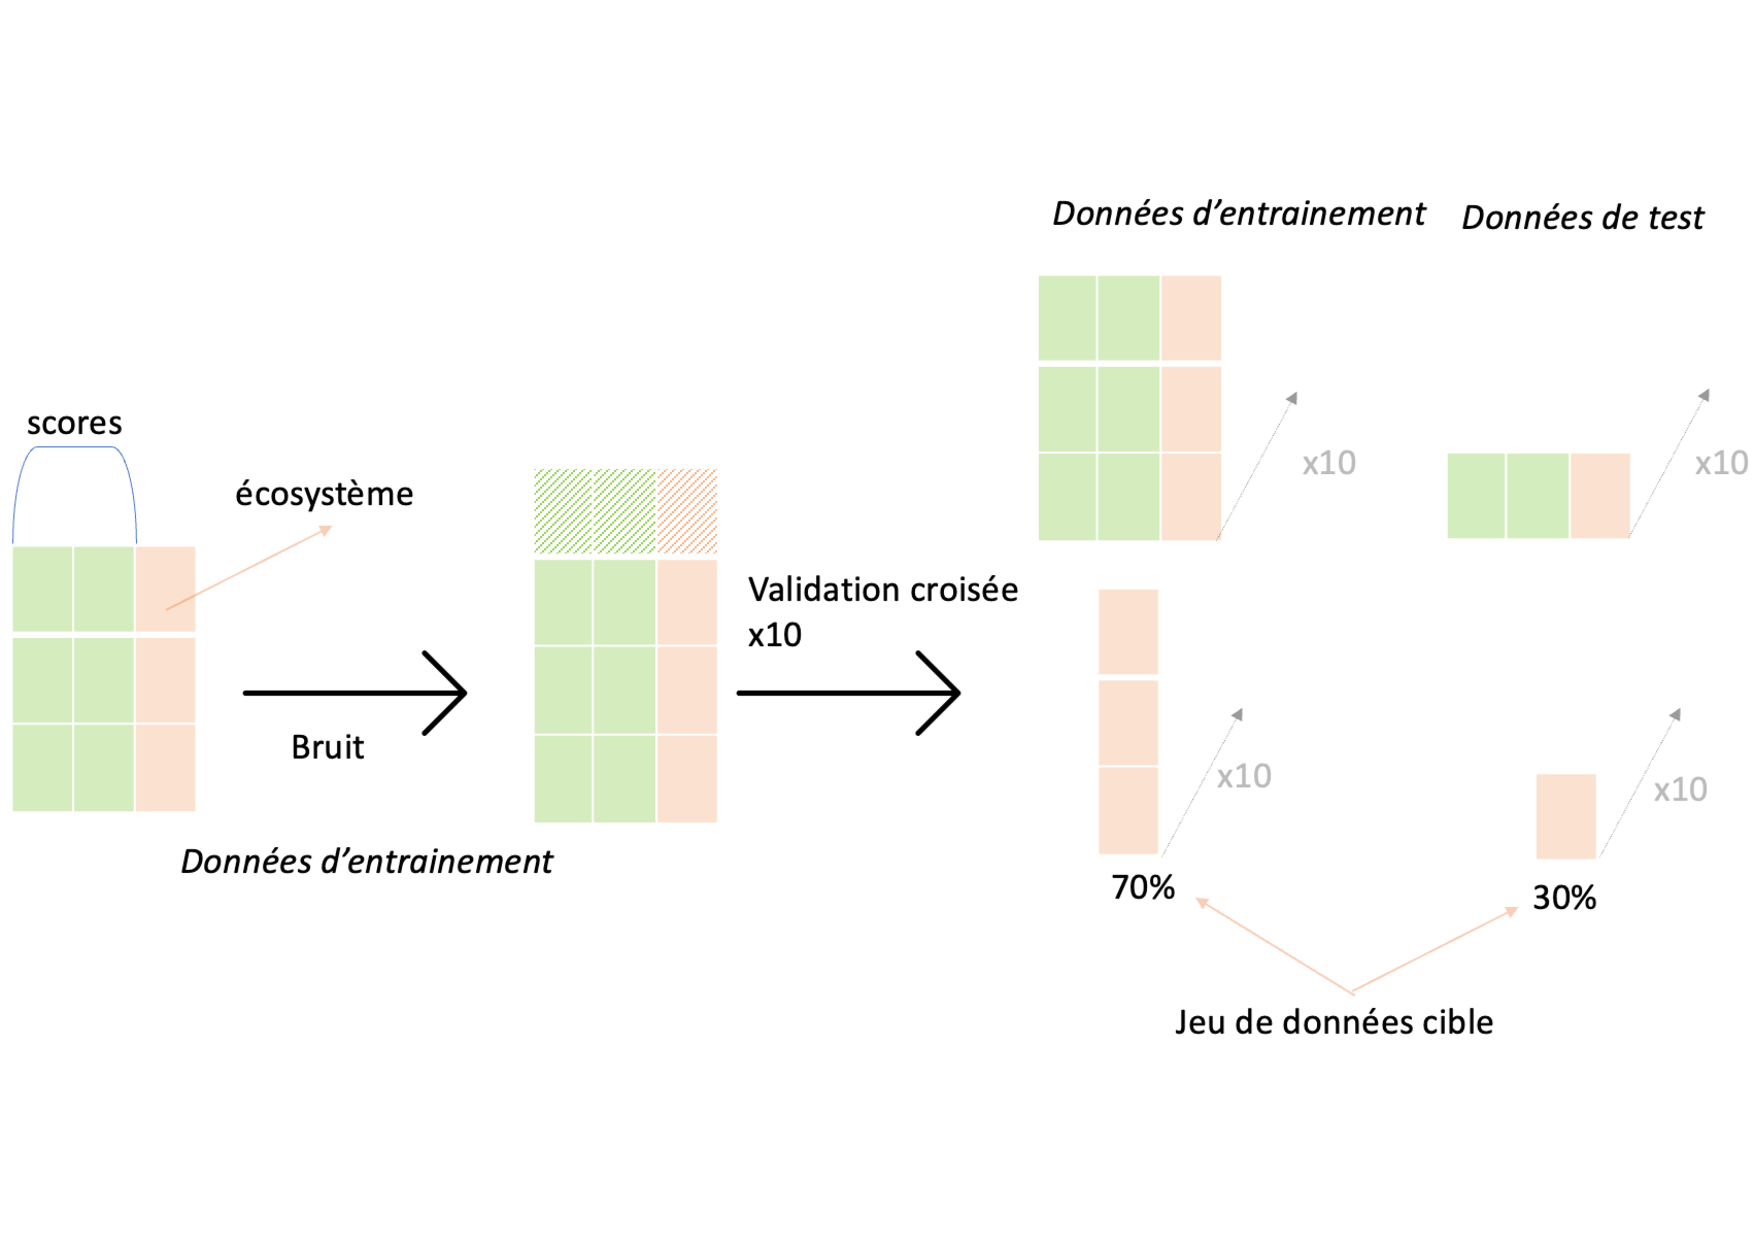
\includegraphics[width=\textwidth]{img/cocomico/svm.pdf}
    \caption{\textbf{Preparation des données afin d'être utilisé par le SVM.} Le jeu de données d'entrainement est constitué du ou des scores d'interaction (en vert) et de l'écosystème associé à ces scores (saumon). Le jeu de donnée cible est consitué de l'écosystème que l'on souhaite prédire.}
    \label{fig:svm}
\end{figure}


En entrée, deux jeux de données sont fournis: un comportant l'écosystème que l'on souhaite prédire (jeu de donnée cible) et le second le ou les scores d'interaction avec leur écosystème (données d'entrainement). Nous avons bruité les données d'entrainement puis effectué 10 validations croisées sur les deux jeux de données. Cela consiste à partitionner aléatoirement 10 fois les jeux de donnée d'entrainement et cibles de la façon suivante: 70\% des jeux de données servent à entrainer le modèle et 30\% servent à le tester. Par exemple, si nous voulons prédire l'écosystème de la feuille à partir du score de coopération, seul le score de coopération sera pris en compte pour l'ensemble des écosystèmes dans les données d'entrainement, et seul l'écosystème de la feuille sera présent dans jeu de donnée cible. 

\paragraph*{Comparaison avec des outils numériques sur des données expérimentales}
Notre approche permet l'analyse de communauté de grande taille, et à ma connaissance, il n'existe pas de méthode qualitative permettant d'évaluer le potentiel de coopération et de compétition à l'échelle de la communauté. Nous avons donc comparé notre approche avec des méthodes numériques de référence basées sur des contraintes: SMETANA \citep{Zelezniak2015} et MiCOM \citep{diener2020}.

Ces deux outils ont été décrit dans le chapitre \ref{ch:edla}. Brièvement, SMETANA propose deux scores pour calculer la coopération  (MIP) et la compétition (MRO) dans une communauté. SMETANA calcule ses scores indépendamment du milieu de culture fourni en entrée et reflète les limites théoriques des interactions \citep{Machado2021}. Nous avons donc lancé SMETANA version 1.2.0 sur 250 communautés composées de 3 à 30 réseaux métaboliques reconstruits avec CarveMe \citep{Machado2018} sur une collection de génomes bactériens de référence du NCBI RefSeq (release 84)\footnote{\url{https://github.com/cdanielmachado/embl\_gems}}. Puis les scores de coopération (MIP) et de compétition (MRO) calculés par SMETANA sont comparés à ceux obtenu avec notre méthode. 

MICOM est originalement développé pour la modélisation du microbiote humain dans lequel des taux de croissances et des flux d'échanges métaboliques sont prédits. Nous avons utilisé MICOM version 0.32.0 sur 188 communautés issues d'une analyse métagénomique, de taille variant de 16 à 98 espèces \citep{diener2020}. Les modèles métaboliques proviennent de la base de données VMH \citep{Noronha.2018} et une curation a été faite sur les réactions de transports. En effet, afin de s'assurer que seules les graines du milieu nutritionnel sont utilisées comme substrat nutritif, nous avons retiré ces réactions des GEMs.  Enfin, nous avons lancé les simulations sur le milieu de culture donné par MICOM: \textit{vmh\_high\_fiber\_agora.qza}. Cependant, MICOM ne donne pas d'indice direct de coopération et de compétition. En utilisant la fonction \texttt{knockout\_taxa} nous avons mesuré l'impact de la perte d'un taxon sur la croissance d'un autre taxon. D'après la documentation de MICOM, une augmentation (resp. une diminution) du taux de croissance après l'étape de knockout indique une coopération (resp. compétition) entre ces deux espèces. En sommant les valeurs positives (resp. négatives), nous avons calculé un pseudo score de compétition (resp. coopération)  à l'échelle de la communauté. \\

Nous avons ensuite comparé les scores calculés par notre approche, ceux de SMETANA et MICOM sur des données réelles. Nous avons récupéré des génomes de souches bactériennes du kéfir \citep{Blasche.2021} et leurs réseaux métaboliques ont été reconstruit avec gapseq version 1.2 \citep{Zimmermann2021} et Pathway-Tools v.25.5 \citep{Karp2022} à l'aide de mpwt v.0.7 \citep{Belcour.2020}. Nous avons également comparé avec les modèles déjà reconstruits par l'outil CarveMe\footnote{\url{https://github.com/cdanielmachado/kefir\_paper}}. Ce jeu de données est composé de 2 communautés: une composée de 23 souches initialement cultivées sur milieu lait liquide et une de 31 souches initialement cultivées sur milieu lait solide; toutes deux contiennent les mêmes nutriments. En utilisant SMETANA, MICOM et notre approche nous avons calculé les potentiels de coopération et de compétition, ainsi que le nombre de métabolites échangeables.

\subsubsection{Implémentation}
Nous avons développé un paquet python nommé \ccmc, de l'anglais \textit{Cooperation and competition in microbial communities}. Le code source est disponible à l'adresse suivante : \url{https://gitlab.inria.fr/ccmc/CoCoMiCo} et est installable avec pypi \href{https://pypi.org/project/CoCoMiCo/}{https://pypi.org/project/CoCoMiCo/}.
Un tutoriel de notre approche a été montré dans un jupyter notebook \footnote{\url{https://gitlab.inria.fr/ccmc/CoCoMiCo/-/blob/dev-0-3/cocomico.ipynb?ref_type=heads}} dans lequel notre approche par raisonnement a été appliquée sur des communautés jouets décrites dans les Figures \ref{fig:concepts} et \ref{fig:scores}. Ce jupyter permet d'explorer les fonctionnalités intéressantes de notre approche, comme l'explicabilité de nos résultats. 

\section{Application et description de notre approche sur des communautés jouets}
Afin de garantir la bonne compréhension de la méthode, nous avons illustré par la Figure \ref{fig:concepts}, les concepts que nous avons décrits. \ccmc permet d'identifier les potentiels de coopération et de compétition au moyen d'un modèle basé sur le raisonnement. Pour y parvenir, l'ensemble des réseaux métaboliques de la communauté ainsi un descriptif du milieu nutritionnel (correspondant aux graines) ont été fourni, afin d'identifier les voies métaboliques activées. La Figure \ref{fig:concepts}a illustre les dépendances nécessaires ainsi que le fonctionnement de \ccmc. Toutes les notions métaboliques que sont: graines, produits, réactants, taxon, communauté et environnement ainsi que les relations entre elles sont montrées dans la sous figure \ref{fig:concepts}b. \\


\begin{figure}[H]
    \centering
    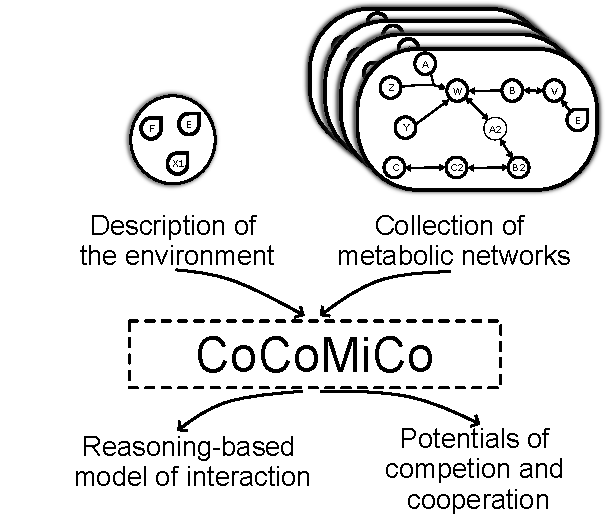
\includegraphics[width=\textwidth]{img/cocomico/concept.pdf}
    \caption{\textbf{Modèle basé sur le raisonnement et son application sur des données jouets.}
     (\textbf{a.}) L'approche générale de \ccmc est décrite. En entrée de l'outil, nous avons besoin d'une collection de GEMs décrivant les organismes présents dans la communauté, ainsi que l'ensemble des graines décrivant le milieu nutritionnel. En sortie, nous obtenons le vocabulaire contrôlé issu des règles logiques nous permettant de calculer les scores de coopération et de compétition.
(\textbf{b.}) Description de la base de faits générée par l'approche par raisonnement et appliquée à cette communauté jouet de 4 GEMs.}
    \label{fig:concepts}
\end{figure}

Pour s'exempter de toute confusion avec un algorithme utilisant seulement la topologie des graphes métaboliques pour l'identification de métabolites d'intérêt, \textit{i.e.} échangeable et limitant, le Figures \ref{fig:mono-polyopsonie} et \ref{fig:scores}a,b représentent la modélisation faite au moyen de l'algorithme d'expansion d'Ebenhoh \citep{Ebenhoh2004}. À partir d'un ensemble de graines, que sont X1, F et E, le \texttt{scope} métabolique de chaque espèce, \textit{i.e.} l'ensemble de composés productibles, est indiqué en jaune dans les Figure \ref{fig:scores}a et b, montrant par la même occasion, les réactions activées par l'intermédiaire des échanges (en bleu) \citep{Frioux2018}. 

\begin{figure}[H]
    \centering
    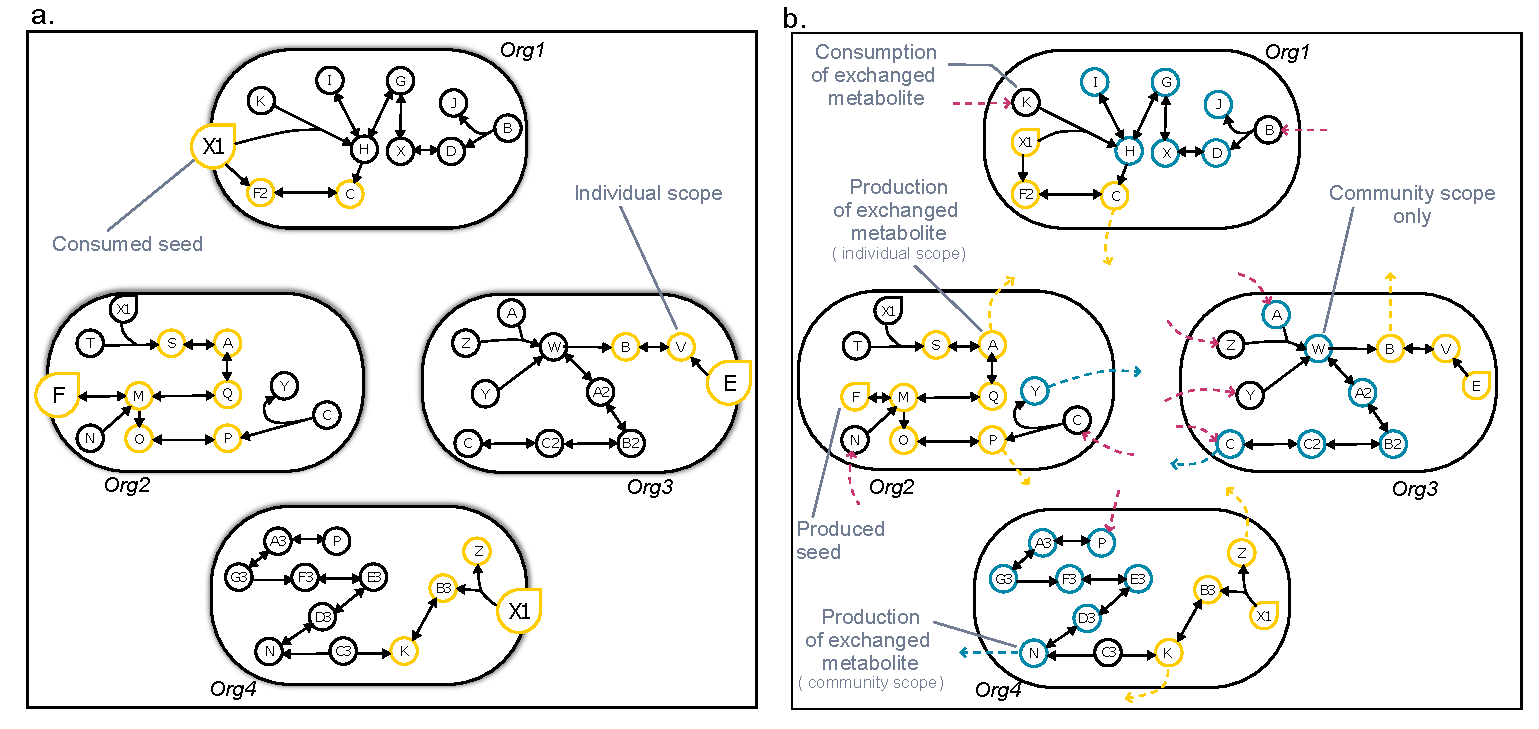
\includegraphics[width=\textwidth]{img/cocomico/score.pdf}
    \caption{  (\textbf{a.}) Potentiel métabolique de chaque GEM de la communauté. Les métabolites en jaune sont les nouveaux métabolites productibles à partir des graines X1, E et F. (\textbf{b.}) Illustration du potentiel métabolique de la communauté. Le potentiel individuel pour chaque GEM est représenté en jaune et le potentiel métabolique de la communauté en bleu, montrant ainsi la plus-value de la communauté. Les flèches sortantes en bleues (resp. jaune) montrent les métabolites échangeables lorsque les GEMs sont en communauté (individuel). Les flèches roses montrent la consommation des métabolites échangés.
    }
    \label{fig:scores}
\end{figure}

Pour cette communauté de taille 4, le \texttt{scope} métabolique de chaque taxon, représenté par le listing \ref{lst:individual-scope}, est donc composé de:

\begin{lstlisting}[mathescape=True,label={lst:individual-scope}, caption={Résultat du scope de chaque taxon},captionpos=b]
Org4: {X1, Z, B3, K}
Org3: {E, V, B}
Org2: {F, M, O, P, Q, A, S}
Org1: {X1, F2, C}
\end{lstlisting}

En communauté, représenté par la sous figure \ref{fig:scores}b, le \texttt{scope} communautaire est composé alors de:
\begin{lstlisting}[mathescape=True,label={lst:individual-scope}, caption={Résultat du scope communautaire},captionpos=b]
% scope metabolique communautaire
Org4: {N, D3, E3, F3, G3, A3, P}
Org3: {C, C2, B2, A2, W, A}
Org2: {Y}
Org1: {J, D, X, G, H, I}
\end{lstlisting}

Le base de connaissance que nous avons décrie nous permet de toujours identifier le taxon associé à la production du métabolite. A l'échelle de la communauté, le \textit{scope} communautaire, montre la plus-value métabolique de la communauté. Pour inférer les scores de coopération et de compétition, \ccmc met en avant les métabolites polyopsonistes, \textit{i.e.} les composés échangés et les graines qui sont co-consommés, et les métabolites monopsonistes, \textit{i.e.} ceux qui sont consommé uniquement que par un organisme. Ces deux concepts sont illustrés dans la Figure \ref{fig:mono-polyopsonie}.

\begin{figure}[H]
    \centering
    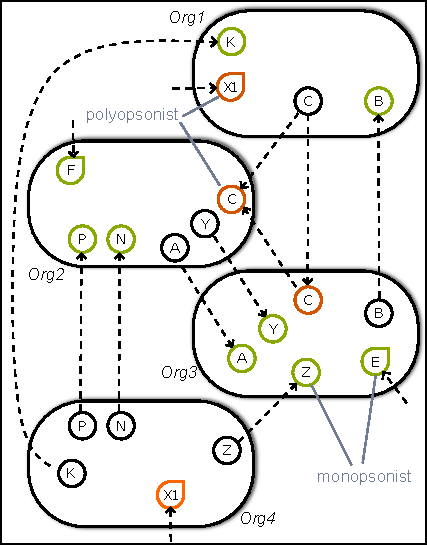
\includegraphics[width=0.6\textwidth]{img/cocomico/poly-monoopsonie.pdf}
    \caption{\textbf{Modèle basé sur le raisonnement et son application sur des données jouets.}
    Résumé des graines prédites comme consommées et des métabolites échangeables. Les éléments considérés comme polyopsonistes sont en orange, où le nombre de GEMs les consommant est strictement supérieur à 1. Ceux en vert traduisent la monoopsonie, un seul GEM les consomme. Pour chaque cas, \ccmc nous informe sur le producteur et le consommateur de chaque métabolite.}
    \label{fig:mono-polyopsonie}
\end{figure}

Ainsi, les métabolites polyopsonistes et monopsonistes sont:
\begin{lstlisting}[mathescape=True,label={lst:individual-scope}, caption={Métabolites considérés comme limitants (polyopsonie) et ceux non limitants (monopsonie)},captionpos=b]
% polyopsonie
X1: {Org1, Org4}
C: {Org2, Org3}

%monopsonie
Org3: {Z, A, Y, E}
Org2: {F, P, N}
Org1: {K}
\end{lstlisting}

En comparaison avec les travaux précédents se basant sur la même approche de raisonnement \citep{Frioux2018}, \ccmc décrit systématiquement les échanges métaboliques ainsi que les substrats limitants afin d'inférer des potentiels de coopération et de compétition à l'échelle de la communauté, que sont respectivement $CooP$ et $ComP$. En plus de cette inférence, deux autres métriques que sont $\delta$ et $\rho$ sont calculées montrant respectivement la plus-value des échanges métaboliques sur le nombre de composés productibles et le nombre de réactions activées grâce aux échanges. \\

Les figures \ref{fig:scores2},\ref{fig:scores3} et \ref{fig:scores4} montrent à travers des exemples, repris en partie des Figures \ref{fig:mono-polyopsonie} \ et  \ref{fig:scores}, les valeurs prises par $CooP$, $ComP$, $\delta$ et $\rho$. À travers ces communautés jouets de différentes compositions taxonomiques et à partir d'un même milieu de culture (E,F et X1), l'évolution des scores face à des perturbations est montrée.  


Dans les sous figures \ref{fig:scores2}a et b, la plus-value de l'organisme 4 est illustrée par les scores calculés par \ccmc. Nous avons observé que seul les scores de coopération ne varient pas, car le nombre de métabolites polyopsonistes et le nombre d'échanges restent identique. Cependant, les deux métriques $\delta$ et $\rho$ informent mécanistiquement sur l'impact de l'organisme 4 par rapport à l'organisme 2. En effet, 5 fois plus de métabolites sont devenus productibles et 10 fois plus de réactions ont été nouvellement activées avec l'organisme 4. Des hypothèses de dépendances métaboliques peuvent être générées ainsi que sur la définition d'une communauté plus coopérative: seul le nombre de métabolites échangé doit-être pris en compte, le score de coopération, sa robustesse à des changements ou encore les plus-values de productions métaboliques.

\begin{figure}[H]
    \centering
    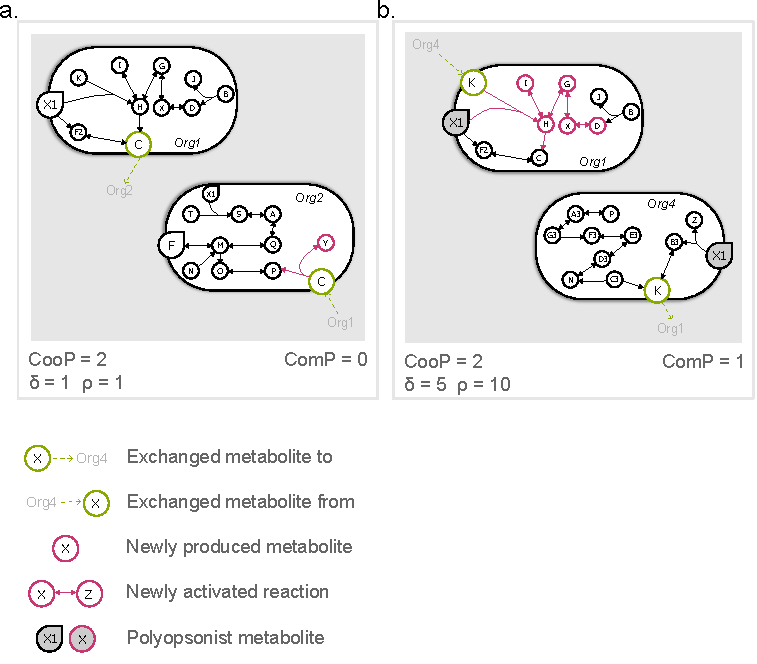
\includegraphics[width=\textwidth]{img/cocomico/score-taille-2.pdf}
    \caption{\textbf{Application de \ccmc sur les exemples jouets} (\textbf{a et b}). L'ensemble des concepts expliqués en amont sont représentés sur cette communauté de taille 2. Les scores de coopération et de compétition, respectivement \textit{CooP} et \textit{ComP}, ainsi que les plus-values métaboliques et réactionnelles, respectivement $\delta$ et $\rho$ sont également représentées. Les composés en verts sont les composés échangésn rose les composés produits grâce aux échanges}
    \label{fig:scores2}
\end{figure}


Dans la Figure \ref{fig:scores3}, la plus-value de l'organisme 4 est également montré dans une communauté de taille 3, dans laquelle, les organismes 1 et 2 sont présents dans les deux cas. Le nombre de substrats polyopsonistes étant identique (2), le score de compétition ne bouge pas, cependant la communauté de la sous figure \ref{fig:scores3}b semble moins coopérative (score de coopération passant de 9 à 8) alors que le nombre de composés échangés reste le même dans les deux cas: 4. Les sous métriques $\rho$ et $\delta$ sont sensiblement identiques. Nous pouvons noter que ces deux communautés de taille 3 semblent moins compétitives que les communautés de taille 2 de la Figure \ref{fig:scores2}, malgré le nombre d'échanges plus important. 

\begin{figure}[H]
    \centering
    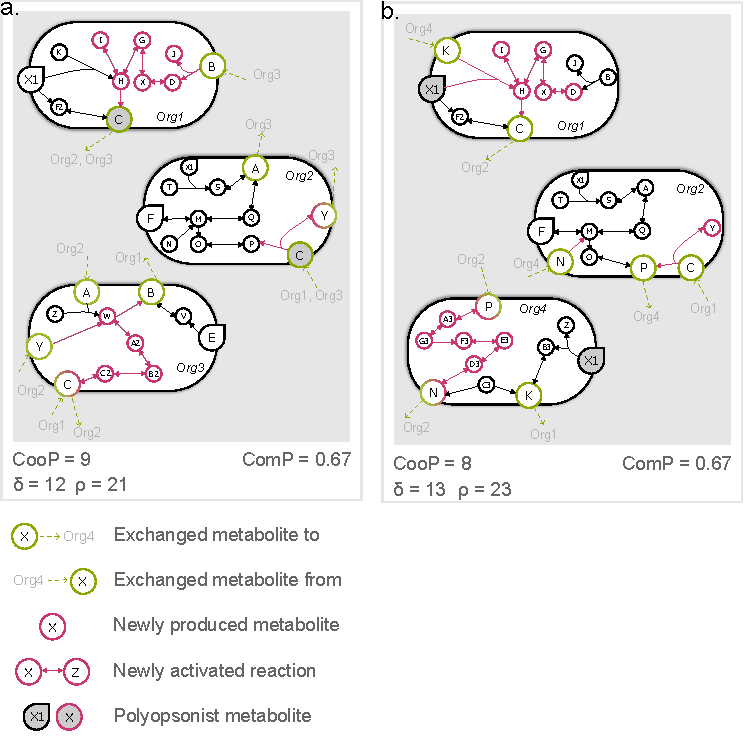
\includegraphics[width=\textwidth]{img/cocomico/score-taille-3.pdf}
    \caption{\textbf{Application de \ccmc sur les exemples jouets} (\textbf{a et b}). L'ensemble des concepts expliqués en amont sont représentés sur cette communauté de taille 3. Les scores de coopération et de compétition, respectivement \textit{CooP} et \textit{ComP}, ainsi que les plus-values métaboliques et réactionnelles, respectivement $\delta$ et $\rho$ sont également représentées.  Les composés en verts sont les composés échangésn rose les composés produits grâce aux échanges}
    \label{fig:scores3}
\end{figure}


Enfin, la Figure \ref{fig:scores4} montre les scores finaux obtenus pour la communauté que nous avons décrits dans les Figures \ref{fig:scores} et \ref{fig:mono-polyopsonie}. Nous pouvons identifier que les organismes 3 et 4 doublent le score de coopération (\textit{cooP} = 17) sans rentrer en compétition (\textit{comP = 1}). 

\begin{figure}[H]
    \centering
    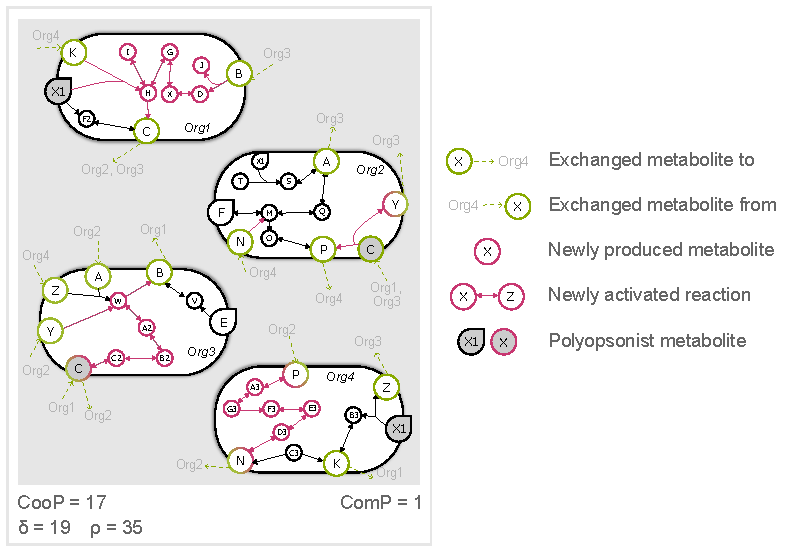
\includegraphics[width=\textwidth]{img/cocomico/score-taille-4.pdf}
    \caption{\textbf{Application de \ccmc sur un exemple jouet} L'ensemble des concepts expliqués en amont sont représentés sur cette communauté de taille 4. Les scores de coopération et de compétition, respectivement \textit{CooP} et \textit{ComP}, ainsi que les plus-values métaboliques et réactionnelles, respectivement $\delta$ et $\rho$ sont également représentées.  Les composés en verts sont les composés échangésn rose les composés produits grâce aux échanges}
    \label{fig:scores4}
\end{figure}


\section{Application de notre approche par raisonnement sur des communautés synthétiques}
Nous venons de décrire le fonctionnement de \ccmc sur des exemples jouets. Des informations plus complètes sont disponibles dans le jupyter notebook écrit à cet effet. \footnote{\url{https://gitlab.inria.fr/ccmc/CoCoMiCo/-/blob/dev-0-3/cocomico.ipynb?ref_type=heads}}

%Un 5ème factice, dénommé mixte, composé des 4 autres écosystèmes.

\subsection{Description des potentiels de coopération et de compétition à travers différents écosystèmes}
Afin de tester nos scores, nous avons appliqué \ccmc sur 50 communautés de taille différentes pour 4 écosystèmes: l'intestin, la feuille, la racine, et le sol.  Pour rappel, nous avons également lancé avec 2 milieux de culture différents: un générique et un spécifique de l'écosystème. Dans les paragraphes suivants, nous étudierons le comportement de nos scores de compétition et de coopération dans les 4 écosystèmes.

\subsubsection*{Application de \ccmc à partir d'un milieu de culture générique}
Une première analyse avec un milieu nutritionnel générique est faite afin de comparer les résultats entre eux, puis une seconde avec un milieu nutritionnel propre à chaque écosystème sera présentée, afin d'identifier l'impact d'un changement de milieu sur les scores d'interaction. \\

Lorsque l'on créé un modèle par raisonnement se basant sur la topologie d'un objet, ici le réseau métabolique, nous devons vérifier si les résultats que l'on obtient ne sont pas directement reliés à cette topologie. Pour cela, nous avons vérifié qu’il n’existe pas de corrélation entre la similarité des réseaux métaboliques et les potentiels de coopération et de compétition.

\paragraph*{Similarité des réseaux métaboliques et potentiels d'interaction}
Notre approche par le raisonnement est une méthode d'inférence qualitative ne permettant pas de calculer flux métaboliques, et se repose donc sur la topologie du modèle métabolique. Nous avons testé la similarité des réseaux en terme de composition en réactions métaboliques calculée par l'indice de Jaccard (voir méthodes) avec les potentiels de coopération et de compétition pour chaque écosystème. La figure \ref{fig:similarite} et la Table \ref{tab:corjacpot} montrent qu'il n'y a pas corrélation entre la topologie des réseaux métaboliques et les potentiels d'interaction obtenus. Ainsi, l'utilisation d'un formalisme discret prenant en compte les conditions environnementales apporte des plus d'informations que la seule structure des réseaux pour analyser et caractériser des communautés bactériennes.

\begin{figure}[H]
    \centering
    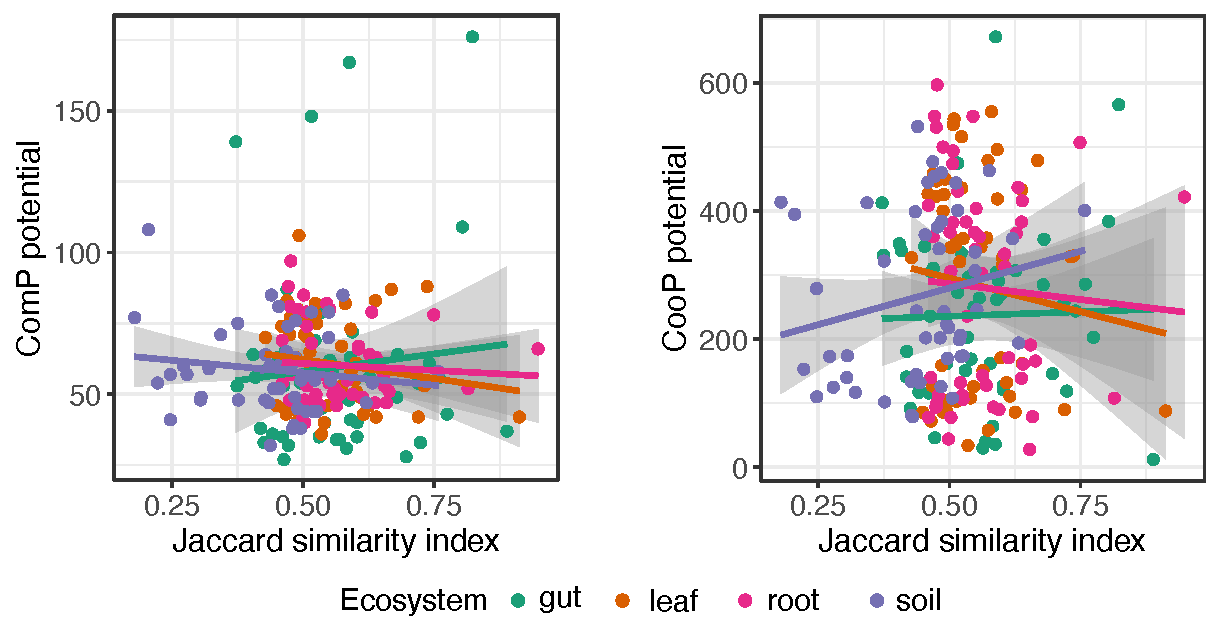
\includegraphics[width=\textwidth]{img/cocomico/similarite.pdf}
    \caption{Scores de coopération et de compétition calculé pour 50 communautés de taille 2 de chaque écosystème. Pour chaque paire, la similarité des réseaux métaboliques a été calculée par l'indice de Jaccard.  Les tests statistiques sont montrés dans la Table \ref{tab:corjacpot}}
    \label{fig:similarite}
\end{figure}

\begin{table*}[h!]
\resizebox{\linewidth}{!}{%
\begin{tabular}{llllllll}
\toprule
          &    & \multicolumn{3}{l}{Competition}    & \multicolumn{3}{l}{Cooperation}    \\ 
ecosystem & n & S        & rho estimate & p. value & S        & rho estimate & p. value \\ 
\midrule
gut       & 50 & 21889.05 &-0.051       & 0.724   & 21128.12 & -0.014      & 0.920 \\
leaf      & 50 & 21483.21 &-0.031       & 0.827    & 23141.56 & -0.111      & 0.441 \\
root      & 50 & 22515.28& -0.081      &0.575    & 23113.31 & -0.109     & 0.447 \\
soil      & 50 & 15744.51 &0.243       & 0.087    & 22505.37 & -0.080      & 0.577 \\
\bottomrule
\end{tabular}%
}
\caption{Résultat des tests de corrélation (Spearman) entre l'indice de similarité de Jaccard et les scores de potentiels d'interaction}
\label{tab:corjacpot}
\end{table*}


\paragraph*{Description globale des potentiels}
Les scores de coopération et de compétition calculés pour chaque écosystème (intestin, sol, racine et feuille) sont représentés par la Figure \ref{fig:ecosystem}. La sous figure \ref{fig:ecosystem}a illustré que les scores varient à la fois selon l'écosystème et à la fois selon la taille de la communauté. En effet, la taille de la communauté est fortement corrélée aux scores d'interaction calculés par \ccmc : (\textsf{ComP}: Spearman $\rho = 0.74$, $P < \num{2.2e-16}$, 
\textsf{CooP}: Spearman $\rho = 0.80$, $P < \num{2.2e-16}$). La forte association avec la coopération n'est pas surprenante, puisque le nombre de voies métaboliques augmente avec l'ajout de nouveaux membres dans la communauté, ainsi que le nombre de métabolites échangeables. Comme la compétition se repose en partie sur le nombre de métabolites échangés, l'augmentation du potentiel de compétition lorsque que la taille de la communauté augmente est attendue. 

Nous avons ensuite testé si, indépendamment de la taille de la communauté, les potentiels de coopération et de compétition de chaque écosystème étaient discernables. Les résultats, illustrés par la sous figure \ref{fig:ecosystem}b, montrent que la compétition semble avoir plus de difficulté à différencier les communautés de la feuille, de la racine et du sol entre eux. Au contraire, le potentiel de coopération, différencie bien la racine et la feuille du sol mais peine à différencier la racine de la feuille.

\begin{figure}[H]
    \centering
    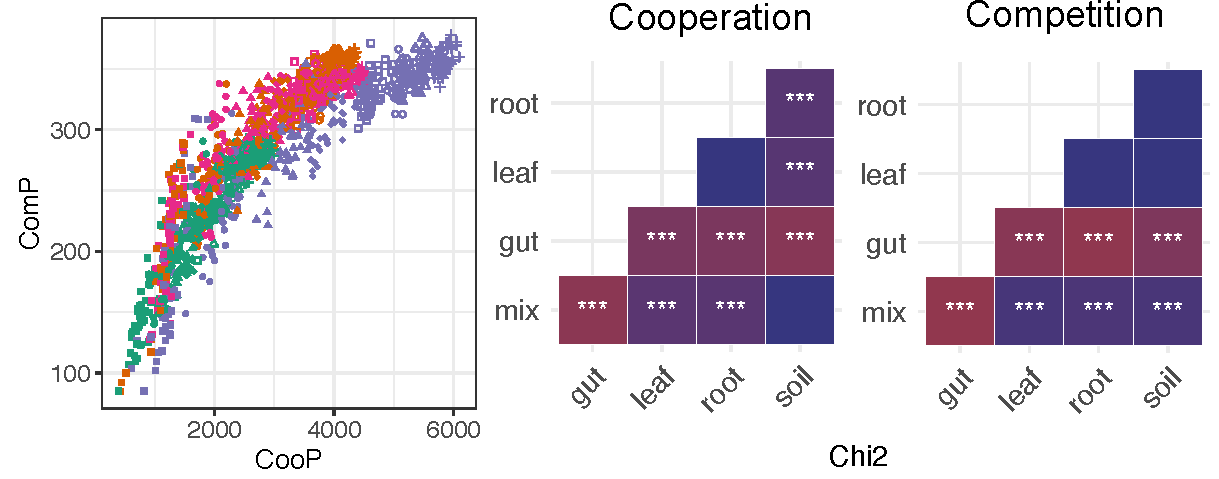
\includegraphics[width=\textwidth]{img/cocomico/coop-comp-ecosys.pdf}
    \caption{(a) Distribution des scores de coopération et de compétition dans des communautés simulées de 5 à 150 bactéries isolées de l'intestin, de la racine, de la feuille et du sol. (b) Résultats d'un test du $\text{chi}^2$ de Kruskal-Wallis comparant les potentiels de coopération et de compétition obtenu en (a) entre écosystème.  (*)  $P$-values ajustées (Benjamini-Hochberg): $P < 0.05$,
    (**) $P$-values ajustées (Benjamini-Hochberg): $P < 0.01$,
    (***) $P$-values ajustées(Benjamini-Hochberg): $P < 0.001$. La communauté \textit{mixte} est un mélange composé équitablement des écosystèmes de la racine, de la feuille, du sol et de l'intestin. }
    \label{fig:ecosystem}
\end{figure}

on observe que, les communautés de l'intestin présentent des scores de compétition et de coopération moins élevé que les autres écosystèmes. Cette observation est explicable par le nombre de métabolites échangés comme indiqué dans Table \ref{table:coop-comp-ecosys} dans laquelle le sol a en moyenne deux fois plus d'échangés que dans les communautés de l'intestin. Nous avons également remarqué que les nombres de métabolites échangés pour la feuille et la racine sont proches. Nous avons supposé que ces résultats pussent être reliés à la diversité taxonomique des GEMs utilisés dans la création des communautés synthétiques (voir Figure \ref{supp:taxo}). Ainsi, au regard de la Figure \ref{supp:taxo}, les communautés du sol et de l'intestin, possédant les plus grandes diversités taxonomiques, ont montré les plus grandes et les plus petites valeurs de compétitions respectivement, suggérant que la diversité taxonomique ne semble pas être le seul facteur déterminant les potentiels d'interaction. En revanche, la similitude des scores d'interaction pour les écosystèmes de la feuille et de la racine, semble être corrélée avec leur diversité taxonomique proche.
%
%
%\begin{table}[H]
%\centering
%\begin{adjustbox}{width=1\textwidth}
%\begin{tabular}{|c|c|c|c|c|c|}
%\hline
% & sol & intestin & racine & feuille & mixte \\
%\hline
%métabolites échangeables & $1024\pm 18$ & $588\pm 33$ & $678\pm 18$ &$693\pm 10$ & $1211\pm 31$ \\
%CooP & $3943\pm 65$ & & & & $4663\pm 115$ \\
%ComP & $263\pm 5$ & & & & $330\pm 9$\\
%
% \hline
%\end{tabular}
%\end{adjustbox}
%\caption{\textbf{Moyenne des scores d'interactions ainsi que du nombre de métabolites échangeables pour tous les écosystèmes et pour une taille de communauté de 150.}}
%\label{table:coop-comp-ecosys}
%\end{table}


\begin{table}[H]
\centering
\begin{adjustbox}{width=1\textwidth}
\begin{tabular}{|c|c|c|c|c|c|}
\hline
 & sol & intestin & racine & feuille & mixte \\
\hline
métabolites échangeables & $\textbf{1516}\pm 27$ & $\textit{709}\pm 45$ & $1171\pm 64$ &$1105\pm 11$ & $\textbf{1525}\pm 53$ \\
CooP & $\textbf{5833}\pm 102$ & $\textit{2739} \pm 175$ & $4361 \pm 137$ & $4273 \pm 40$ & $\textbf{5877}\pm 189$ \\
ComP & $\textbf{355}\pm 9$ & $\textit{276} \pm 11$ & $345 \pm 3$ & $\textbf{357} \pm 4$ & $\textbf{384}\pm 12$\\

 \hline
\end{tabular}
\end{adjustbox}
\caption{\textbf{Moyenne des scores d'interactions ainsi que du nombre de métabolites échangeables pour tous les écosystèmes et pour une taille de communauté de 150.}}
\label{table:coop-comp-ecosys}
\end{table}

Afin de vérifier statistiquement nos observations, nous avons comparé les scores de compétition et de coopération pour chaque taille et par écosystème (voir Figure \ref{fig:diff-potentials})

\begin{figure}[H]
    \centering
    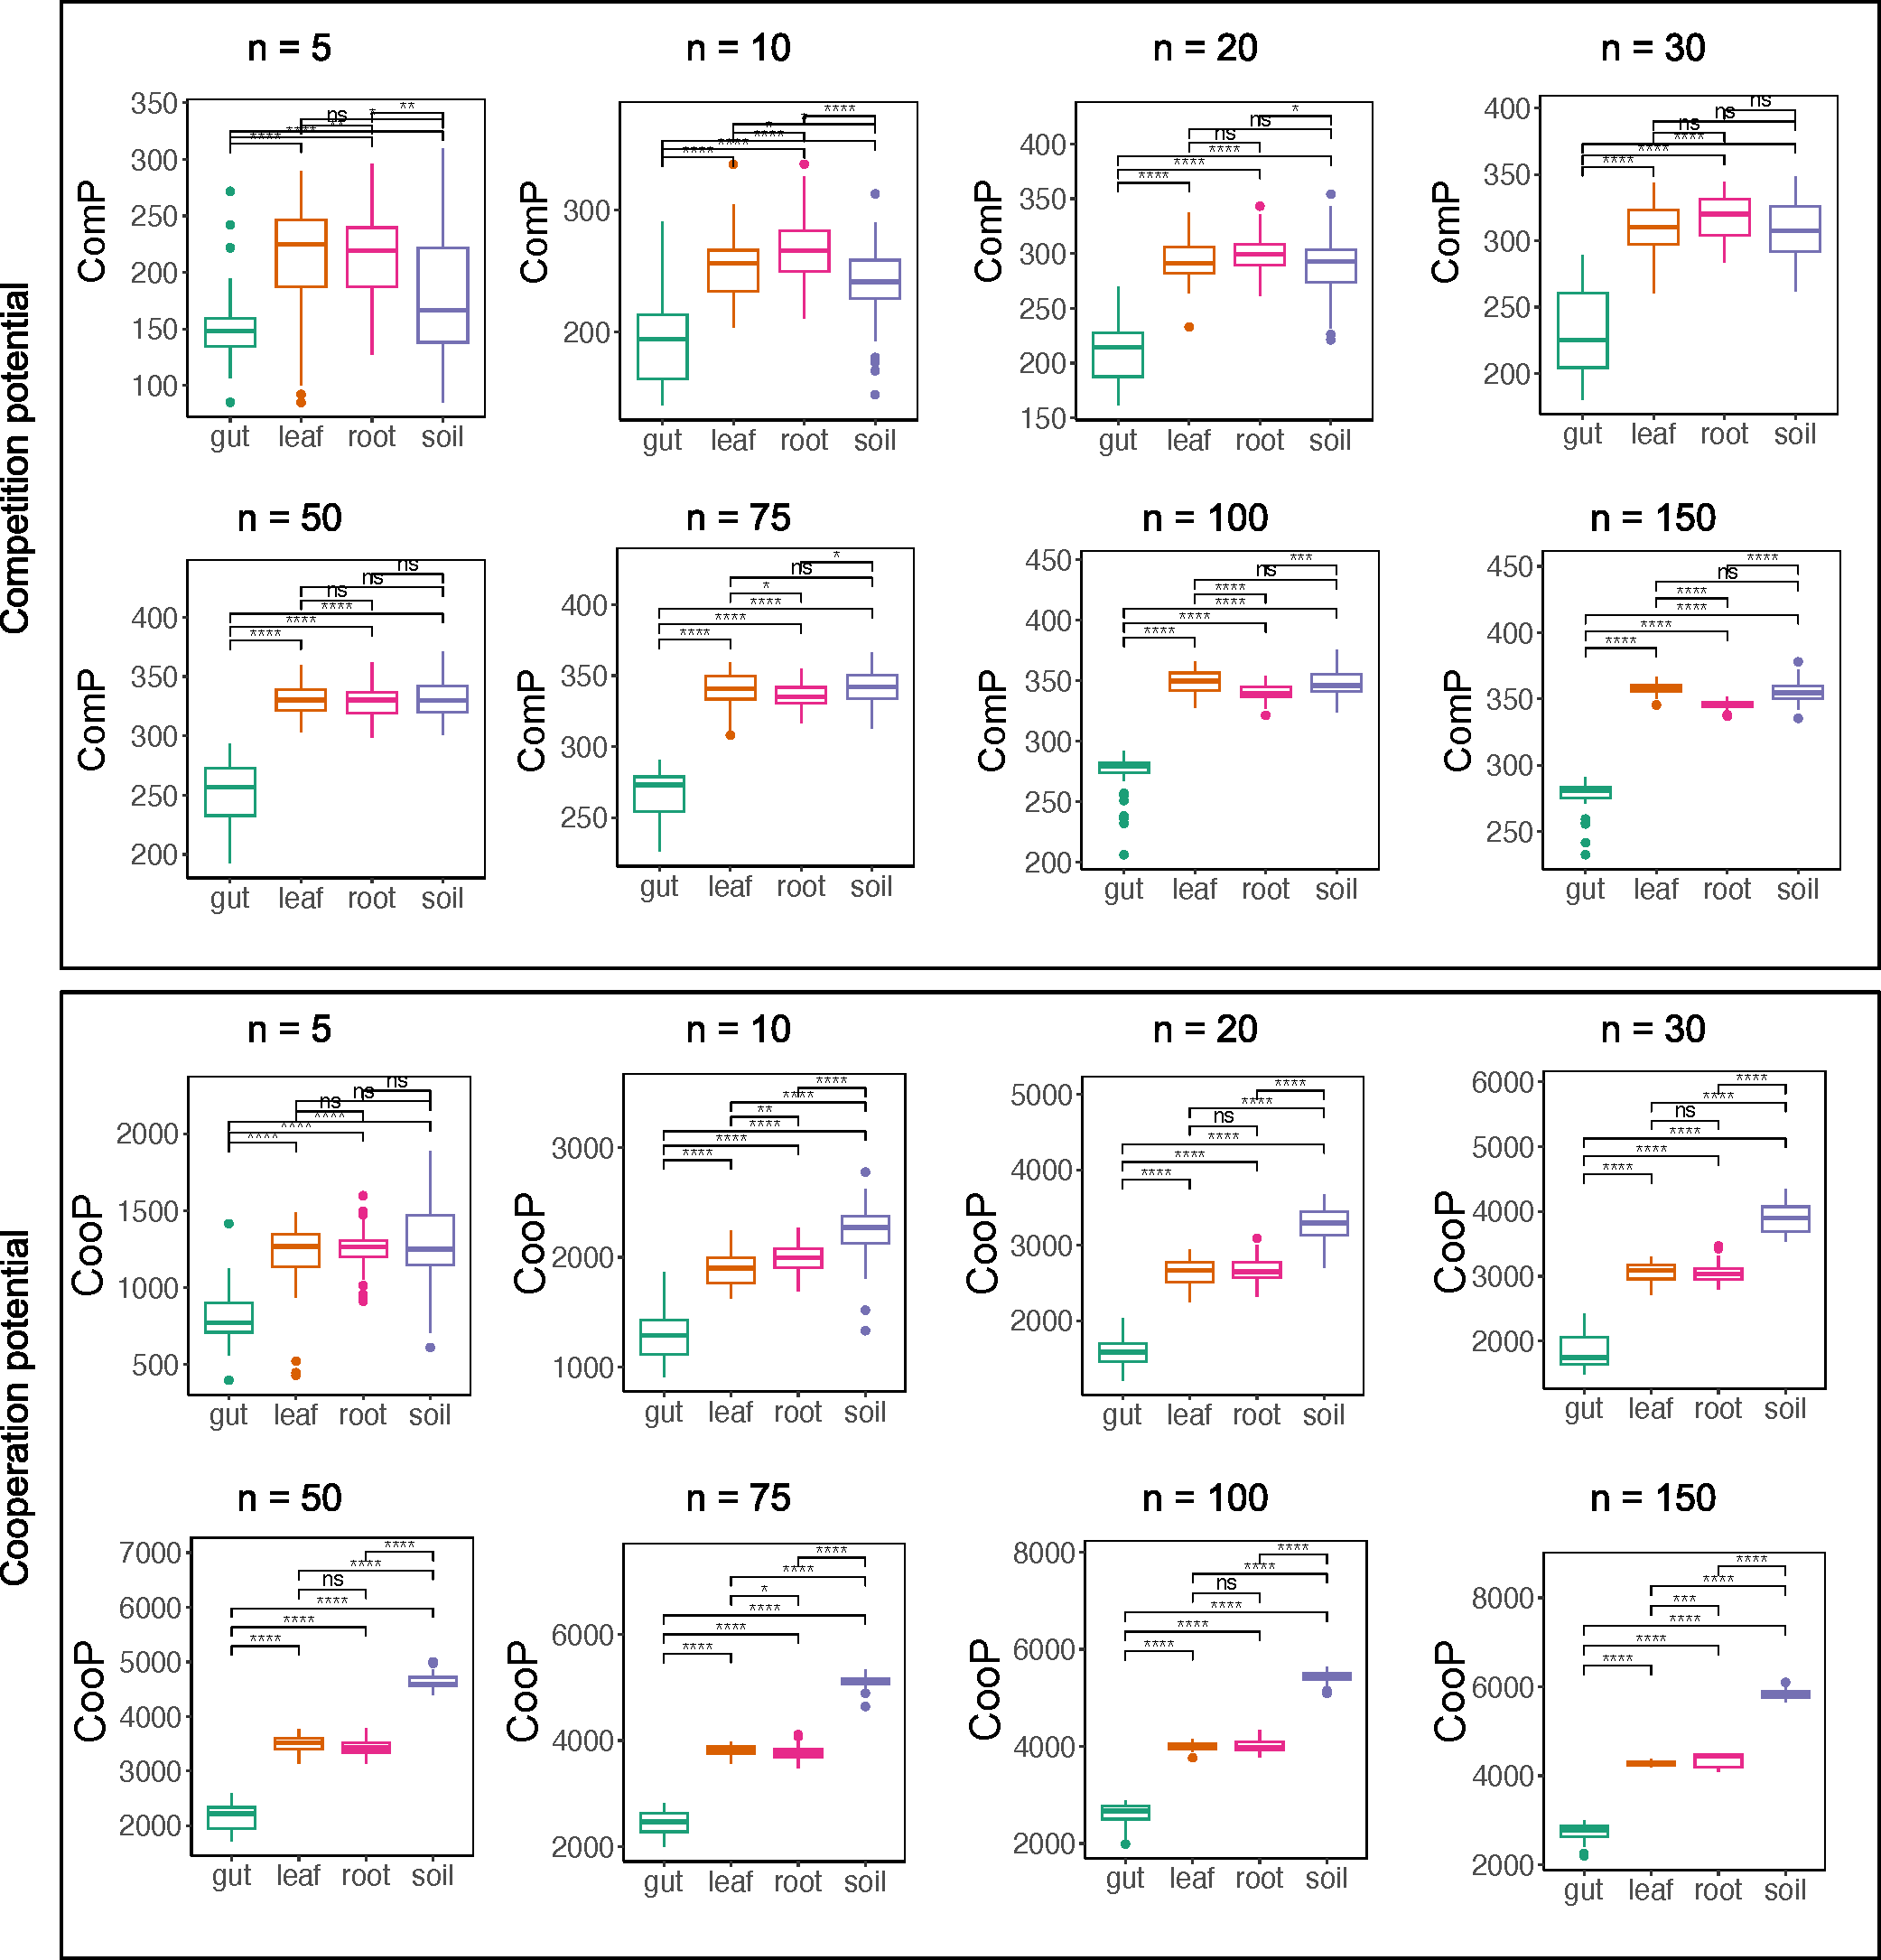
\includegraphics[width=\textwidth]{img/cocomico/ecosysteme_diff_potentials.pdf}
    \caption{Distribution des scores de coopération et de compétition dans des communautés simulées de 5 à 150 bactéries isolées de l'intestin, de la racine, de la feuille et du sol. Une comparaison de moyenne avec le test de Wilcoxon a été faite. (*)  $P$-values ajustées (Benjamini-Hochberg): $P < 0.05$,
    (**) $P$-values ajustées (Benjamini-Hochberg): $P < 0.01$,
    (***) $P$-values ajustées(Benjamini-Hochberg): $P < 0.001$.}
    \label{fig:diff-potentials}
\end{figure}

Nous montrons que la compétition distingue globalement moins bien les communautés de petites tailles (entre 5 et 30), surtout entre les écosystèmes de la racine, de la feuille et du sol, ce qui est cohérent avec les observations décrites plus haut. Le score de coopération semble être plus apte à discerner des communautés > 10 taxa, sauf entre les écosystèmes de la feuille et de la racine. Les communautés de grandes tailles étant plus réalistes, ces dernières sont distinguées par nos potentiels d'interactions, apportant de la confiance à nos métriques. \\

Un point nouveau, et peu documenté dans la littérature était la mesure de l'impact d'une modification de la composition bactérienne sur les scores de coopération et de compétition. Notre approche ne pouvant prendre en compte des abondances, nous avons modélisé l'impact d'un changement discret en ajoutant ou en enlevant une nouvelle espèce dans chacune des communautés de tailles 3 à 150 de l'intestin (voir Figure \ref{fig:added-value}). Par rapport à la communauté originale, les scores de coopération et de compétition ne permettent plus de distinguer la plus-value d'ajouter ou de retirer une espèce à partir d'une communauté de taille 10. Cela suggère donc que l'effet d'une modification d'un facteur biotique peut-être capturé par \ccmc uniquement pour des écosystèmes de petites tailles. Les communautés de tailles réelles ne verront pas leurs potentiels d'interactions changés significativement.


\begin{figure}[H]
    \centering
    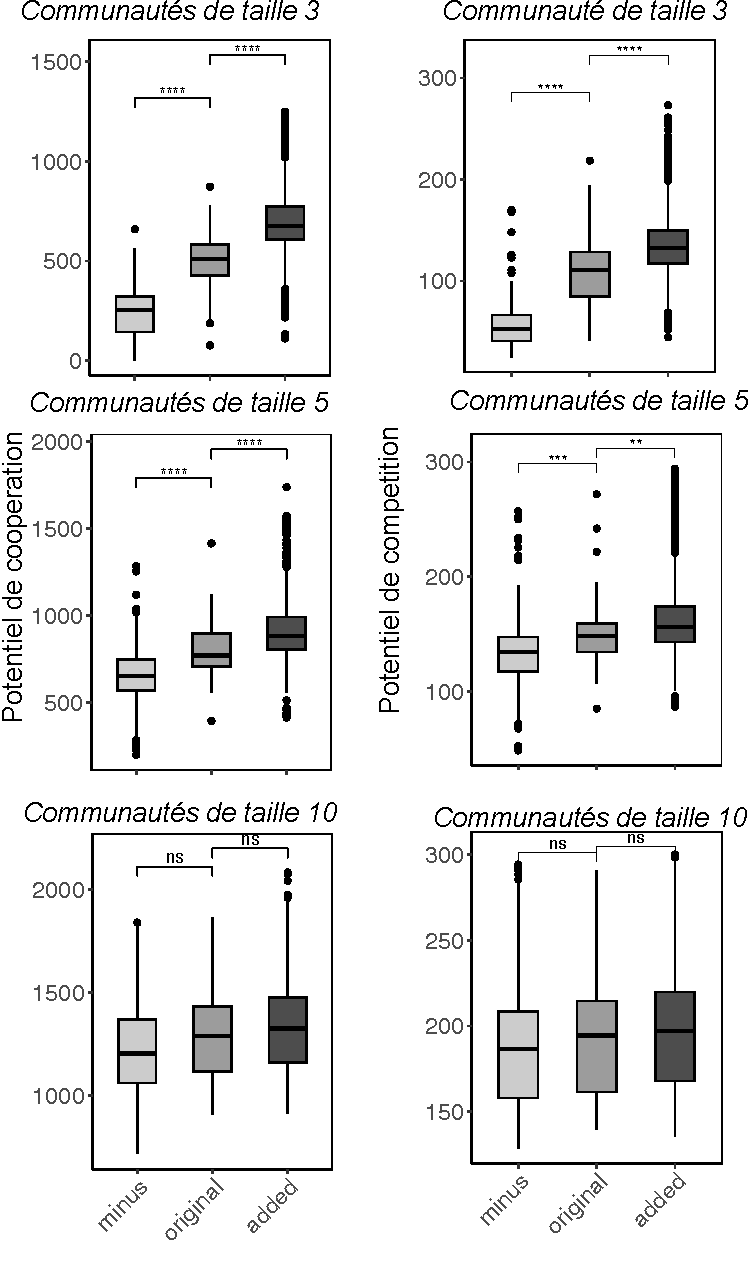
\includegraphics[width=0.8\textwidth]{img/cocomico/added-value.pdf}
    \caption{Effet d'ajouter ("added") ou de retirer une espèce ("minus") sur les potentiels de coopération et de compétition pour chaque communauté. Le test de comparaison de moyenne Wilcoxon a été utilisé sur des communauté de taille 3 à 10 sur l'écosystème de l'intestin.}
    \label{fig:added-value}
\end{figure}

\paragraph*{Comparaison des potentiels d'interaction propres aux écosystèmes avec ceux d'un écosystème factice}

Nous avons en plus créé une $5^{\grave{e}me}$ communauté artificielle composée d'une combinaison des réseaux métaboliques appartenant aux 4 autres écosystèmes, dénotée "mixte". Cette communauté non réaliste permet de vérifier que les potentiels de coopération et de compétition sont spécifiques aux écosystèmes, et permettrait donc de discerner des communautés non plausibles. Nous avons remarqué que le potentiel de compétition a permis de distinguer l'écosystème mixte des autres, ce qui n'est pas le cas pour le score de coopération où le sol et un écosystème factice serait similaire du point de vue de ce potentiel d'interaction (voir Figures \ref{fig:ecosystem} et \ref{fig:diff-potentials}). Nous retrouvons également ce résultat dans la Table \ref{table:coop-comp-ecosys} où les valeurs de coopération, de compétition et du nombre de métabolites échangés sont particulièrement proche de l'écosystème du sol.  Lorsque l'on compare par taille de communauté (voir Figure \ref{fig:mix-diff-potentials}) les deux potentiels de coopération et de compétition arrivent à différencier l'écosystème factice. En revanche, comme illustré dans la Figure \ref{fig:ecosystem}, l'écosystème du sol et le mixte semblent être identique de point de vue de la coopération.

\begin{figure}[H]
    \centering
    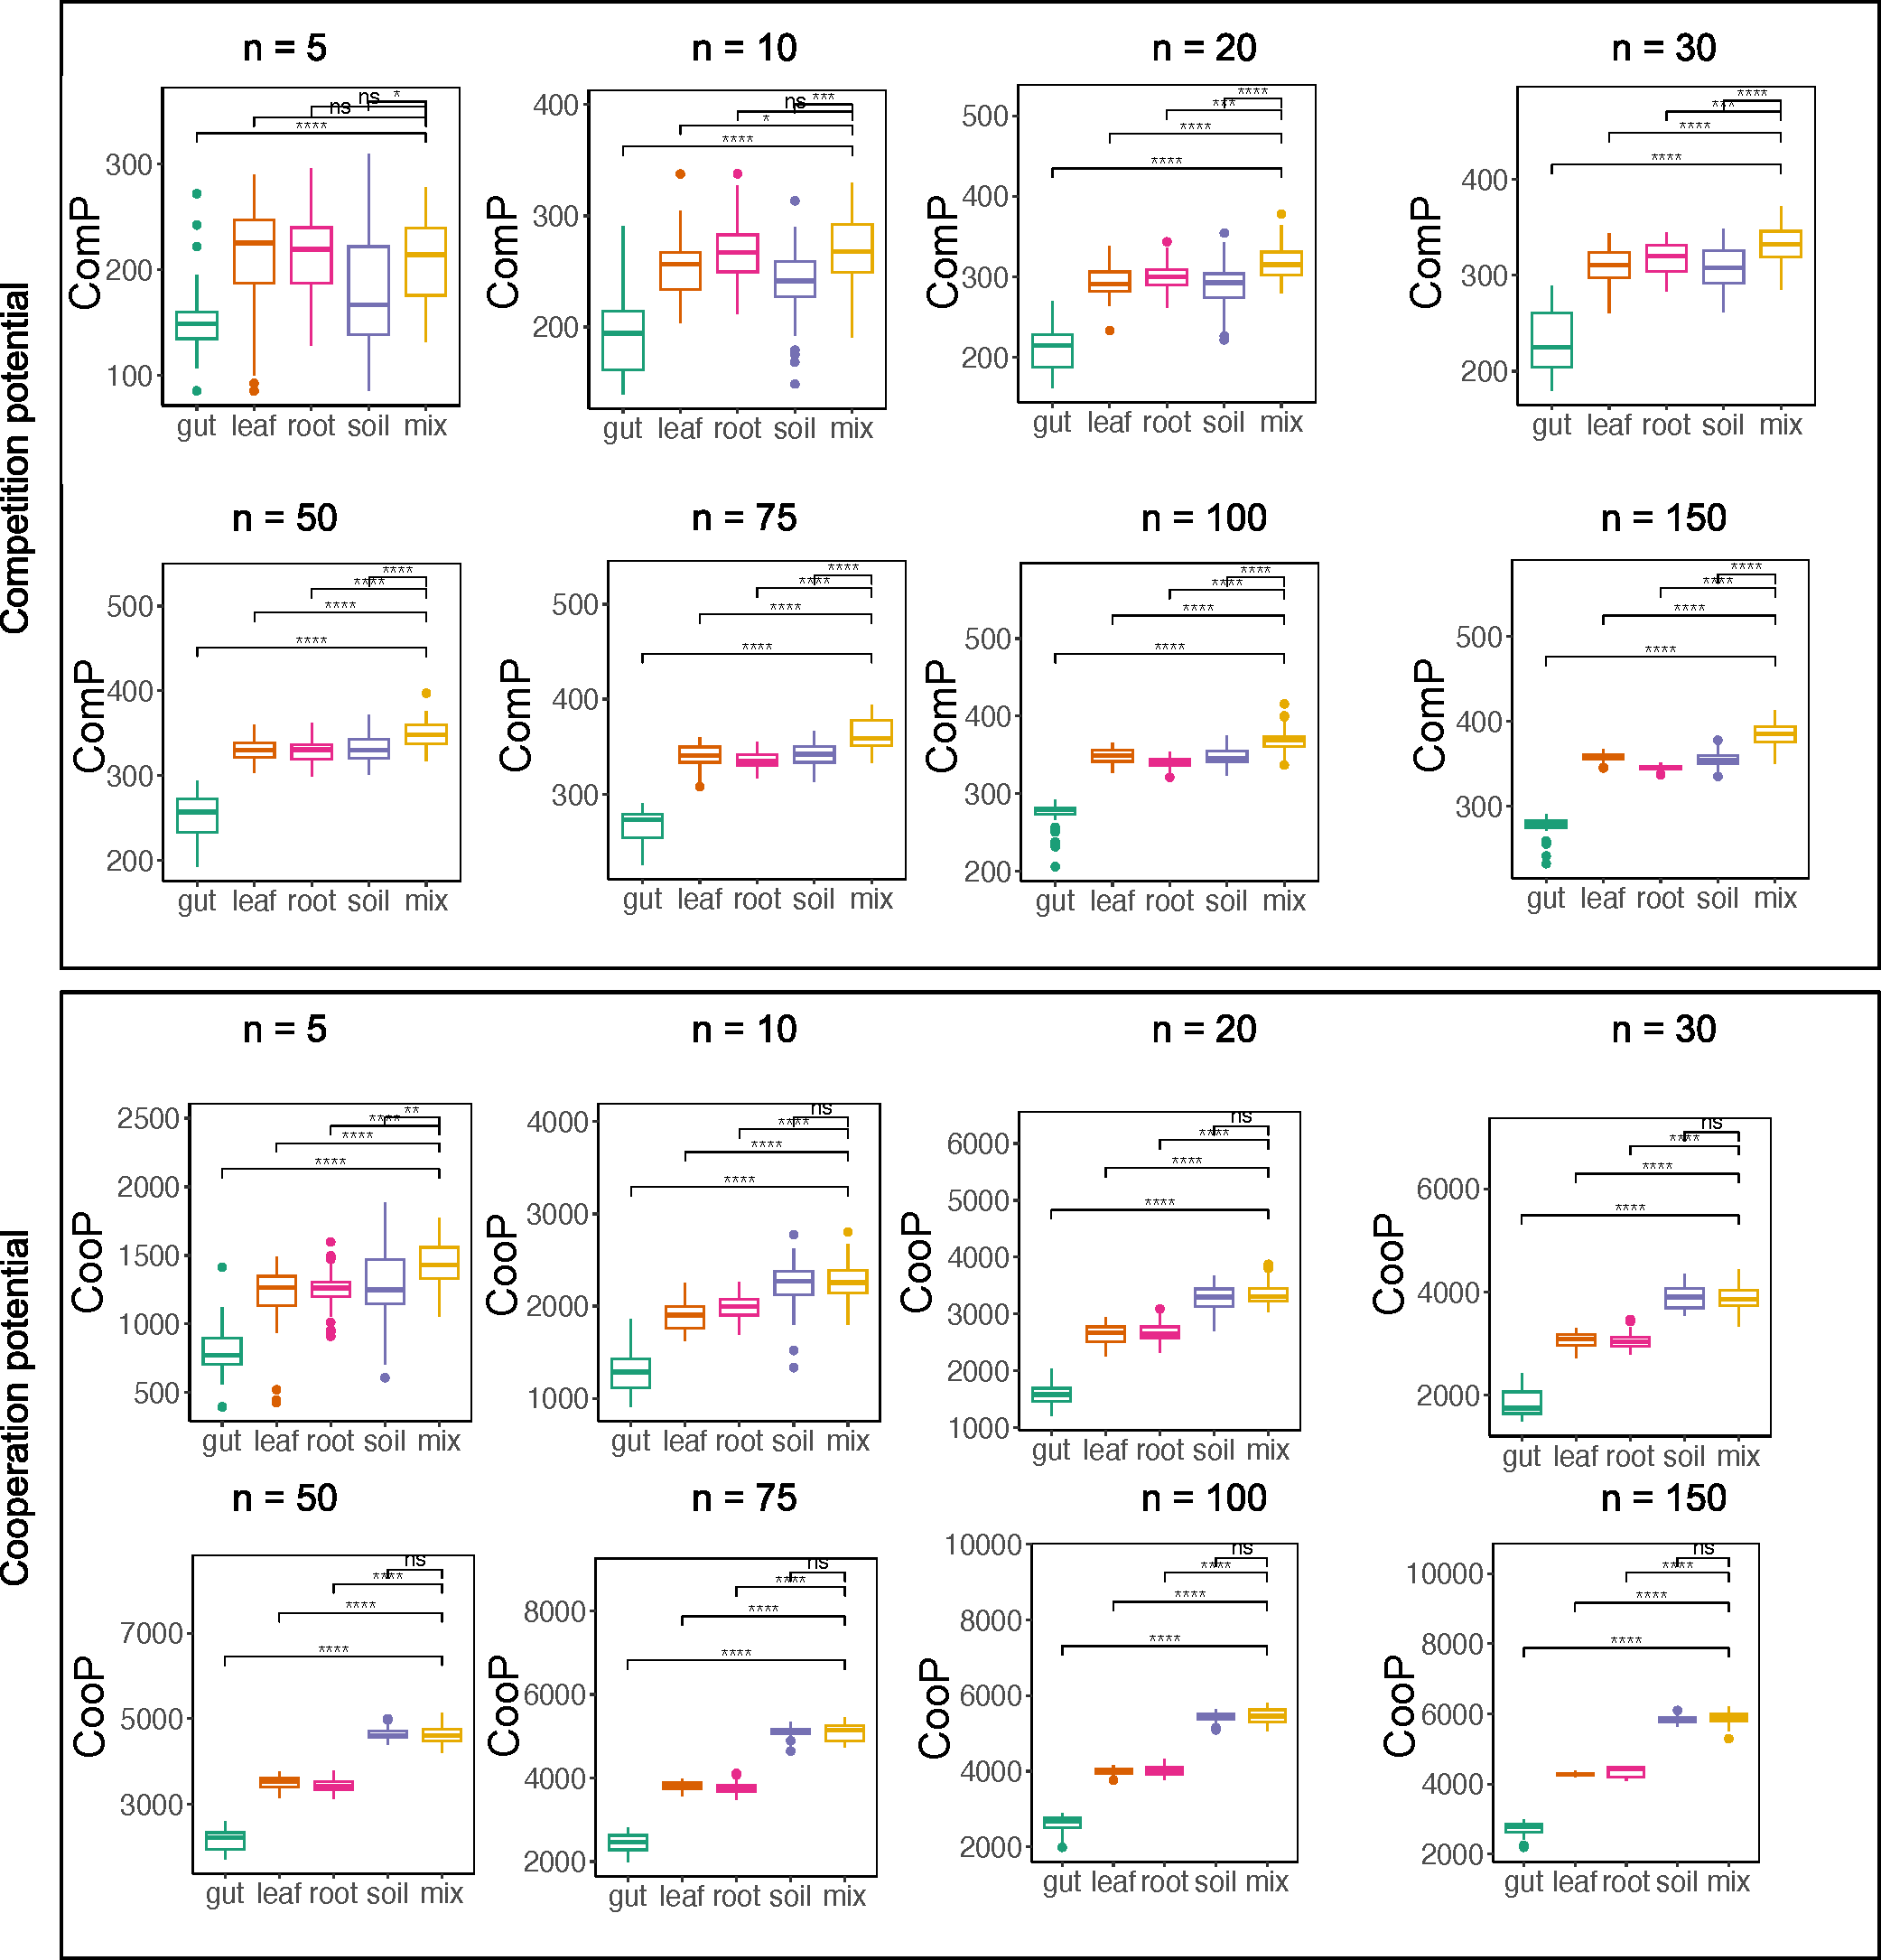
\includegraphics[width=\textwidth]{img/cocomico/mix_ecosystem_diff_potentials.pdf}
    \caption{Distribution des scores de coopération et de compétition dans des communautés simulées de 5 à 150 bactéries isolées de l'intestin, de la racine, de la feuille, sol et du mixte. Seule une comparaison deux à deux avec le mixte a été faite. La comparaison de moyenne est faite avec le test de Wilcoxon. (*)  $P$-values ajustées (Benjamini-Hochberg): $P < 0.05$,
    (**) $P$-values ajustées (Benjamini-Hochberg): $P < 0.01$,
    (***) $P$-values ajustées(Benjamini-Hochberg): $P < 0.001$}
    \label{fig:mix-diff-potentials}
\end{figure}



Une étape terminale d'exploitation des potentiels d'interaction serait de pouvoir prédire des écosystèmes à partir d'un score de coopération et de compétition. Les résultats de ce test sont présentés dans le paragraphe suivant.

\paragraph*{Prédiction d'écosystème à partir de potentiel d'interaction}
Nous avons vu et démontré que les potentiels d'interaction semblent être en général spécifiques à des écosystèmes. Une hypothèse sous-jacente consiste à se demander si, à partir des potentiels d'interaction de coopération et de compétition de chaque écosystème, il est possible de prédire l'écosystème correspondant. Afin de tester et vérifier cette hypothèse, nous avons utilisé un SVM ( de l'\textit{anglais}, Support Vector Machine) non linéaire (voir méthodes). Les résultats sont présentés par la Table \ref{table:SVM}.



\begin{table}[h!]
\centering
\begin{adjustbox}{width=1\textwidth}
\begin{tabular}{|c|c|c|c|c|}
\hline
 & sol & intestin & racine & feuille\\
\hline
CooP & $0.67\pm 0.34$ & $\textbf{0.74}\pm \textbf{0.32}$ & $0.48\pm 0.34$& $0.53\pm 0.35$ \\
ComP & $0.40\pm 0.31$ & $\textbf{0.93}\pm \textbf{0.12}$ &$0.44\pm 0.29$ & $0.42\pm 0.23$\\
ComP et CooP & $\textbf{0.71}\pm\textbf{ 0.29}$ & $\textbf{0.74}\pm \textbf{0.32}$ & $0.49\pm 0.35$&$0.5\pm 0.39$\\

 \hline
\end{tabular}
\end{adjustbox}
\caption{Résultat de prédiction des écosystèmes de la racine, de la feuille, du sol et de l'intestin, à partir les graines génériques. Les colonnes correspondent aux écosystèmes que l'on souhaite prédire à partir d'uniquement le score de coopération (CooP), d'uniquement le score de compétition (Comp) ou une combinaison des deux (ComP et CooP).}
\label{table:SVM}
\end{table}

Nous pouvons voir qu'à partir des graines génériques, seul l'intestin semble pouvoir être prédit correctement par les 3 combinaisons de scores. Le score de compétition semble plus se démarquer avec une moyenne de 0.93. Ce chiffre peut être intéprété comme un probabilité d'obtenir le bon résultat. Ainsi, un score de 0.93 signifie que nous avons 93\% de chance de prédire l'écosystème de l'intestin à partir du score de compétition. L'écosystème du sol semble être uniquement prédictible avec une combinaison du score de coopération et de compétition. En revanche, prédire les écosystèmes de la feuille et de la racine ne semble être faisable. Une hypothèse pouvant expliquer cette observation est la diversité taxonomique de ces deux écosystèmes qui n'est pas suffisamment distincte et génère des potentiels métaboliques proches, ayant pour conséquence des scores d'interaction similaires.


\subsubsection*{Application de \ccmc à partir d'un milieu de culture spécifique}
Nous avions utilisé un milieu de culture générique pour toutes les communautés pour comparer les potentiels d'interaction entre eux. Afin d'identifier une possible gamme des potentiels de coopération et de compétition propre à chaque écosystème, un milieu de culture spécifique de l'intestin et un milieu commun aux 3 autres écosystèmes ont été générés. 

\begin{figure}[H]
    \centering
    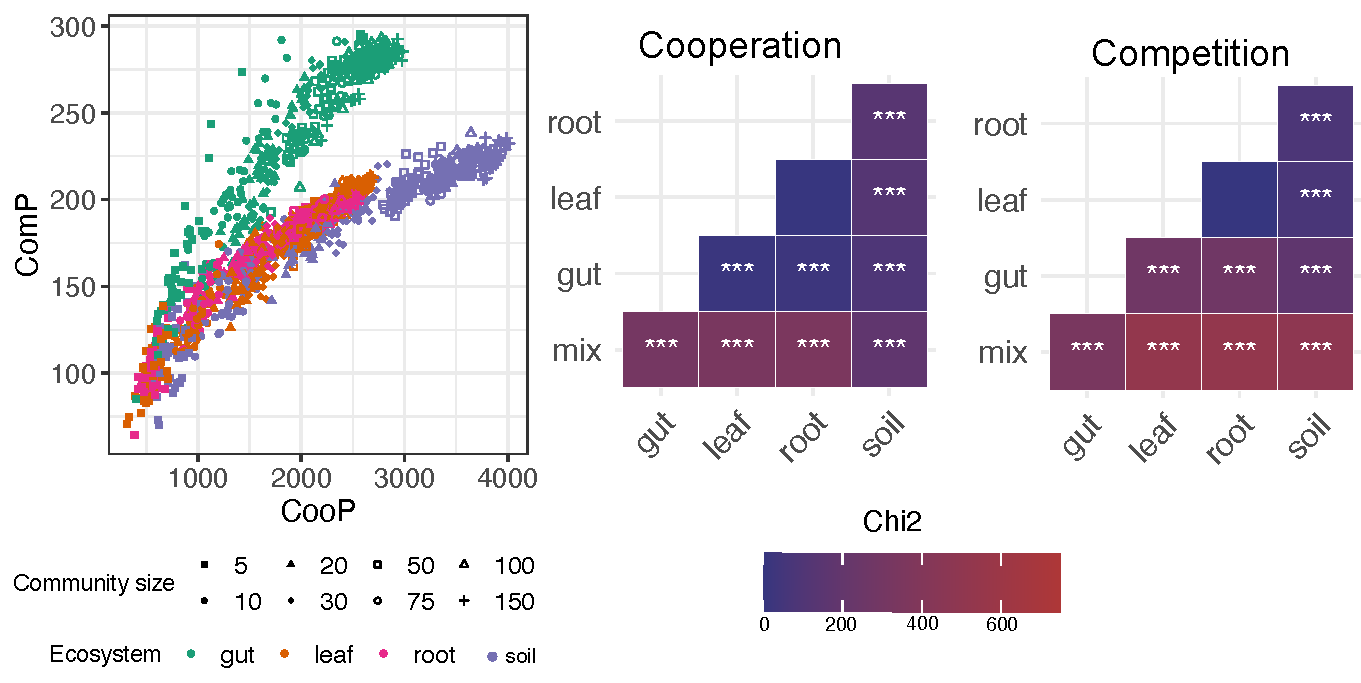
\includegraphics[width=\textwidth]{img/cocomico/coop-comp-ecosys-specific.pdf}
    \caption{(a) Distribution des scores de coopération et de compétition dans des communautés simulées de 5 à 150 bactéries isolées de l'intestin, de la racine, de la feuille et du sol. (b) Résultats d'un test du $\text{chi}^2$ de Kruskal-Wallis comparant les potentiels de coopération et de compétition obtenu en (a) avec ceux de la communauté mixte. }
    \label{fig:ecosystem-specific}
\end{figure}

Il existe des différences notables entre la Figure \ref{fig:ecosystem-specific}, utilisant environnement nutritionnel spécifique et la Figure \ref{fig:ecosystem}, utilisant un milieu générique. L'intestin semble avoir des scores de compétitions plus importants, et la valeur maximale de coopération est réduite à 4000 contre 6000 dans la Figure \ref{fig:ecosystem}. Lorsque l'on compare les potentiels de coopération et de compétition sans tenir compte de la taille de la communauté, les deux potentiels distinguent presque tous les écosystème. En effet, la racine et la feuille ne semble pas être significativement différent. Malgré cette amélioration, les potentiels d'interaction ne permettent toujours pas de prédire correctement des écosystèmes (voir Table \ref{table:SVM-specific})\\


\begin{table}[h!]
\centering
\begin{adjustbox}{width=1\textwidth}
\begin{tabular}{|c|c|c|c|c|}
\hline
 & sol & intestin & racine & feuille\\
\hline
CooP & $\textbf{0.90}\pm \textbf{0.15}$ & $0.48\pm0.23$ & $0.56\pm 0.37$& $0.47\pm 0.34$ \\
ComP & $0.66\pm 0.25$ & $\textbf{0.96}\pm \textbf{0.04}$ &$0.63\pm 0.39$ & $0.49\pm 0.33$\\
ComP et CooP & $\textbf{0.79}\pm\textbf{ 0.29}$ & $\textbf{0.87}\pm \textbf{0.15}$ & $0.59\pm 0.40$&$0.44\pm 0.35$\\

 \hline
\end{tabular}
\end{adjustbox}
\caption{Résultat de prédiction des écosystèmes de la racine, de la feuille, du sol et de l'intestin, à partir les graines spécifiques. Les colonnes correspondent aux écosystèmes que l'on souhaite prédire à partir d'uniquement le score de coopération (CooP), d'uniquement le score de compétition (Comp) ou une combinaison des deux (ComP et CooP). }
\label{table:SVM-specific}
\end{table}

Le résultat de la Table \ref{table:SVM-specific} indique qu’il n’est toujours pas possible de déterminer le potentiel d'interaction permettant de prédire un écosystème. Cependant, la combinaison des deux scores ainsi que l'utilisation de graines spécifique, semblent permettre la prédiction de l'intestin et du sol avec plus de confiance.

\subsection{Comparaison avec des méthodes basées sur des contraintes et application à des données expérimentales}


Les résultats précédents ont montré une application \textit{in silico} des potentiels d'interaction. Dans la suite de ce chapitre, nous allons présenter deux cas d'étude utilisant des données de communautés pour analyser leurs potentiels de coopération et de compétition. Dans le premier cas, nous avons calculé les potentiels d'interaction avec \ccmc sur 250 communautés créés artificiellement, de taille 3 à 30 et comparé avec les scores obtenus par SMETANA. Puis, sur un jeu de données de MICOM, nous avons calculé les potentiels de coopération et compétition avec \ccmc sur 188 communautés issues d'une analyse métagénomique, allant d'une taille 16 à 98 et comparé ces potentiels avec ceux calculés avec MICOM. Dans le second cas, nous avons comparé les résultats de coopération et de compétition obtenus par MICOM, SMETANA et \ccmc sur 2 communautés du kéfir provenant de \citep{Blasche.2021}.

\subsubsection*{Comparaison de méthodes numériques dans le calcul de score d'interaction}
Dans cette section, nous présenterons les résultats de la première étude de cas. L'objectif est vérifié, pour une même communauté, si nos scores sont corrélés avec ceux d'outils reconnus de la littérature.
La première remarque est que notre score de coopération semble être corrélé avec les scores des méthodes numériques avec une corrélation avec un $\rho = 0.8$ et une p-value de $2.2^{-16}$ pour SMETANA et $\rho = 0.69 $ avec une p-value de $2.2^{-16}$ pour MICOM (voir Figure \ref{fig:ccmc-micom-smetana}).

\begin{figure}[H]
    \centering
    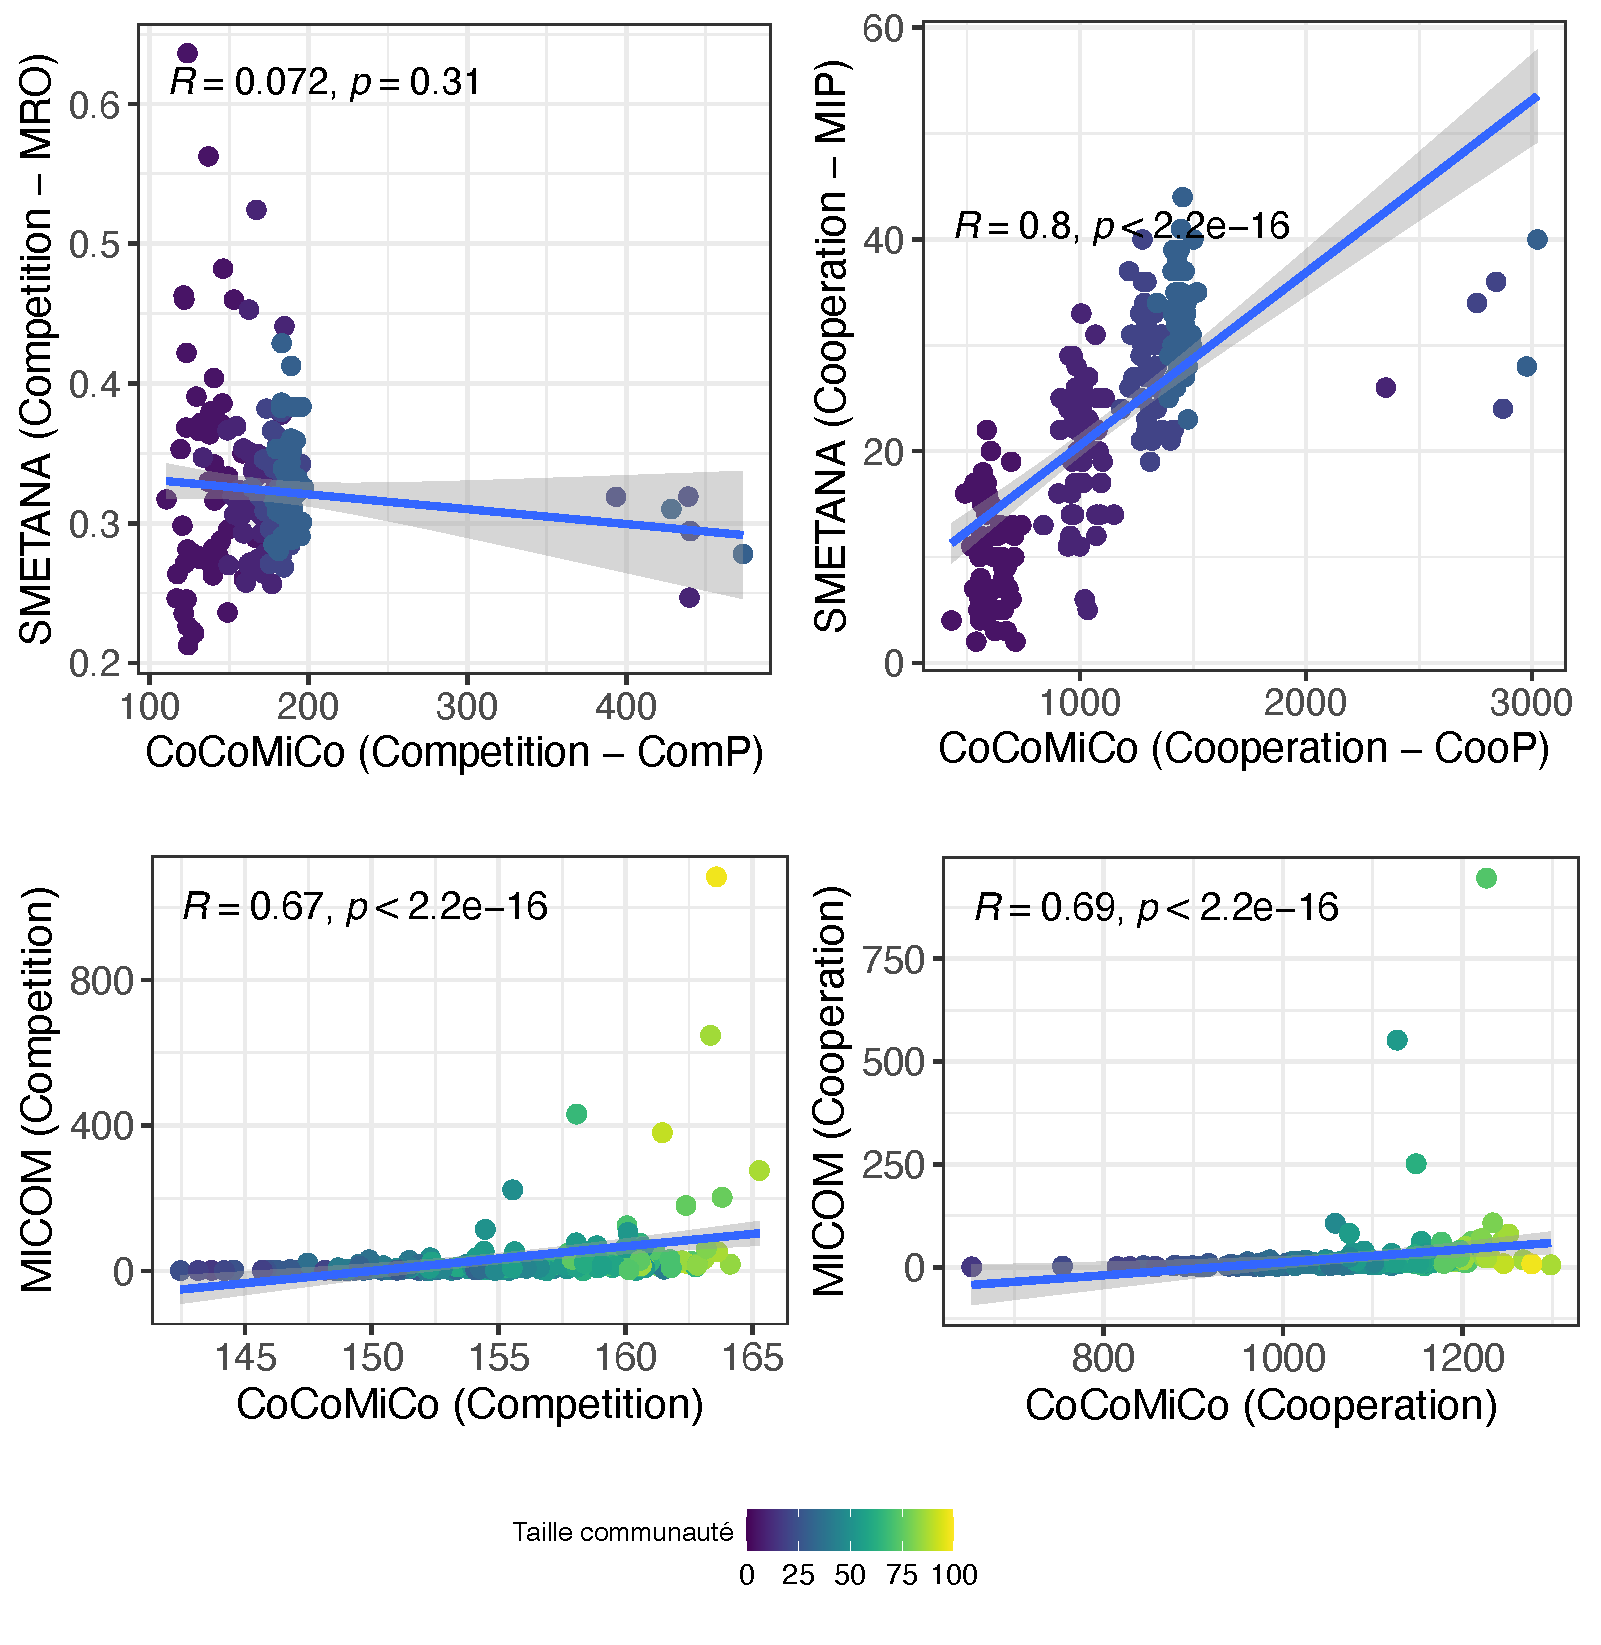
\includegraphics[width=\textwidth]{img/cocomico/ccmc-micom-smetana.pdf}
    \caption{\textbf{Comparaison des approches numériques MICOM et SMETANA avec notre approche}. (a) Comparaison des scores de coopération et de compétition développé par SMETANA,  respectivement MIP et MRO. 250 communautés de taille 3 à 30 ont été générées aléatoirement. (b) Comparaison des scores de coopération et de compétition \textit{ad hoc}  de MICOM sur 188 communautés issues d'analyses métagénomiques de taille 16 à 98 GEMs. En (a) et en (b), les corrélations ont été calculées avec la corrélation de Spearman.}
    \label{fig:ccmc-micom-smetana}
\end{figure}

La compétition en revanche, est seulement corrélée avec le score MICOM avec un $\rho$ de 0.67 et une p-value de $2.2^{-16}$. L'absence de corrélation avec le score SMETANA ($\rho$ de 0.072 avec une p-value de $0.31$) peut-être expliqué par la prise en compte d'un milieu de culture théorique minimum. Et donc, SMETANA ne prend pas en considération l'ensemble des éléments nutritifs comme dans \ccmc et MICOM. \\



Un point non négligeable à notifier est le temps de calcul des approches numériques. SMETANA ne pouvait être utilisé sur des communautés de taille supérieure à 30 pour une allocation mémoire de 10G. MICOM quant à lui, a permis l'analyse de grande communautés (98) mais met plusieurs heures pour une communauté avec 20G de mémoire. En comparaison, \ccmc a mis environ 3 minutes pour analyser une communauté de taille 150 avec 10G de mémoire.
De ce fait et malgré les différences méthodologiques, nous avons observé des similitudes et une rapidité d'exécution de \ccmc permettant la comparaison de potentiels de coopération et de compétition de communautés rapidement. De plus, les corrélations avec MICOM nous encouragent dans cette direction pour améliorer la précision des scores d'interaction.


\subsubsection*{Application sur des données expérimentales du kéfir}
Nous avons appliqué \ccmc ainsi que les deux approches numériques MICOM et SMETANA sur 2 communautés du kéfir de tailles différentes, 23 et 31. Lors de l'analyse des communautés sur milieu lait, les auteurs et autrices montrent un réseau d'interaction plus dense et globalement négatif pour la plus grande communauté, cultivé sur du gel d'agarose (noté lait-solide). L'ensemble des résultats est présenté dans la Table \ref{tab:kefirpotentials}. Tout d'abord, les réseaux métaboliques de Pathways-Tools étant dépourvus d'une fonction de biomasse nativement, l'application d'une méthode numérique était donc infaisable. 


\begin{table*}[h!]
\centering
\begin{adjustbox}{width=1\textwidth}
\begin{tabular}{cccccccc}
\toprule[1.3pt]
& \multicolumn{1}{c}{\multirow{2}{*}{Communauté}}   & \multicolumn{2}{c}{Pathway Tools}             & \multicolumn{2}{c}{CarveMe}                   & \multicolumn{2}{c}{gapseq}                                                                   \\
%\midrule[1.5pt]
        & & \multicolumn{1}{c}{Coopération} & Compétition & \multicolumn{1}{c}{Coopération} & Compétition & \multicolumn{1}{c}{Coopération} & Compétition                                               \\
\midrule[1pt]
\multicolumn{1}{c}{\multirow{2}{*}{CoCoMiCo}} & lait-liquide    & \multicolumn{1}{c}{{\begin{tabular}[c]{@{}l@{}} 1090.68 \\ (287) \end{tabular}}}           &     \multicolumn{1}{c}{123.26}         & \multicolumn{1}{c}{{\begin{tabular}[c]{@{}l@{}}2183.06 \\ (426) \end{tabular}}}     & {149.65}      & \multicolumn{1}{c}{{\begin{tabular}[c]{@{}l@{}}2039.34\\ (520) \end{tabular}}}            &     \multicolumn{1}{c}{233.74}         \\ \Cline{0.2pt}{2-8}
\multicolumn{1}{c}{} & lait-solide & \multicolumn{1}{c}{{\begin{tabular}[c]{@{}l@{}}1098.85\\ (278) \end{tabular}}}            &      \multicolumn{1}{c}{124.5}        & \multicolumn{1}{c}{{\begin{tabular}[c]{@{}l@{}}2651.19\\ (497) \end{tabular}}}     & {152.74}       & \multicolumn{1}{c}{{\begin{tabular}[c]{@{}l@{}}2039.39\\ (499) \end{tabular}}}            &      \multicolumn{1}{c}{243.53}                                 \\
\midrule[1pt]
\multicolumn{1}{c}{\multirow{2}{*}{SMETANA}} & lait-liquide    & \multicolumn{1}{c}{-}            &   \multicolumn{1}{c}{-}          & \multicolumn{1}{c}{{\begin{tabular}[c]{@{}l@{}}22\\ (59) \end{tabular}}}         & {0.329}       & \multicolumn{1}{c}{NA}            &      \multicolumn{1}{c}{{0.682}}    \\ \Cline{0.2pt}{2-8}
 \multicolumn{1}{c}{} & lait-solide & \multicolumn{1}{c}{-}            &   \multicolumn{1}{c}{-}          & \multicolumn{1}{c}{{\begin{tabular}[c]{@{}l@{}}22\\ (66) \end{tabular}}}           & {0.348}       & \multicolumn{1}{c}{NA}            &       \multicolumn{1}{c}{{0.693}}                               \\
\midrule[1pt]
\multicolumn{1}{c}{\multirow{2}{*}{MICOM}}  & lait-liquide    & \multicolumn{1}{c}{-}            &     \multicolumn{1}{c}{-}        & \multicolumn{1}{c}{{\begin{tabular}[c]{@{}l@{}}24.75\\ (99) \end{tabular}}}      & \multicolumn{1}{c}{{2.75}}        & \multicolumn{1}{c}{{\begin{tabular}[c]{@{}l@{}}22.435\\ (95) \end{tabular}}}           &       \multicolumn{1}{c}{{22.432}}      \\ \Cline{0.2pt}{2-8}
\multicolumn{1}{c}{} & lait-solide & \multicolumn{1}{c}{-}            &     \multicolumn{1}{c}{-}        & \multicolumn{1}{c}{{\begin{tabular}[c]{@{}l@{}}34.80\\ (109) \end{tabular}}}      & \multicolumn{1}{c}{{3.8}}         & \multicolumn{1}{c}{{\begin{tabular}[c]{@{}l@{}}31.476\\ (103) \end{tabular}}}            &        \multicolumn{1}{c}{{31.454}}                             \\
\bottomrule[1.3pt]
\end{tabular} 
\end{adjustbox}
\caption{\textbf{\ccmc,Smetana et MICOM sont appliqués sur les données expérimentales du kéfir \citep{Blasche.2021}} Les potentiels de coopération et de compétition sont obtenus pour les deux communautés cultivées sur lait liquide (n=23) ou lait solide (n=31) à partir des réseaux métaboliques reconstruits avec Pathway Tools, CarveMe et gapseq, et analysés MICOM, SMETANA et CoCoMiCo. Sans besoin d'une fonction objective, seul \ccmc a su déterminer les potentiels d'interaction sur les réseaux métaboliques issus de Pathway-Tool. SMETANA n'a pas pu déterminer le score de coopération signifiant qu'au moins une bactérie n'a pas pu pousser dans le modèle de communauté.
}
\label{tab:kefirpotentials}
\end{table*}


Globalement, les scores de potentiels de coopération et de compétition sont tous plus importants dans la plus grande communauté, facteur sûrement déterminé par la grande corrélation des scores avec la taille de la communauté (cf Figure \ref{fig:ecosystem}). Le nombre de métabolites échangés est moindre pour la plus petite communauté et pour les réseaux reconstruits avec Pathway-Tools et gapseq. Le réseau d'interaction positive 2 à 2 étant plus dense dans cette communauté, le nombre d'échanges métaboliques est attendu comme plus important. Les réseaux reconstruits avec CarveMe montrent l'inverse suggérant donc que la méthode de reconstruction peut impacter des propriétés intrinsèques à la communauté (ici, le nombre d'échanges).
Enfin, dernier point, notre méthode basée sur le raisonnement décrit un nombre de métabolites échangés nettement plus important que pour MICOM et SMETANA. Cela est également attendu puisque notre approche identifie toutes les interactions potentielles sans optimisation numérique. 

\section{Discussion et conclusion}
Dans ce chapitre nous avons proposé une méthode permettant d'analyser des communautés naturelles de façon rapide mettant en avant la coopération et la compétition. L'une des grandes forces de notre approche et son adaptabilité. En effet, l'obtention de réseaux métaboliques de bonnes qualité n'est pas courante dans l'analyse haut-débit de communautés microbiennes. Cette qualité vient d'une curation manuelle approfondie issue de la connaissance extraite de la littérature ou d'expériences \textit{in vitro}.  Ainsi, les réseaux métaboliques sont au stade d'ébauche et déterminer une réaction de biomasse peut être compliqué. Cependant, une approche comme \ccmc permet d'obtenir un aperçu des potentiels métaboliques de la communauté, ainsi que ses possibles interactions.  En revanche, permettre à l'utilisateur ou l'utilisatrice d'effectuer ou non une optimisation sur une fonction objective de son choix serait une amélioration pertinente pour la méthode. \\

L'inférence à grande échelle de mécanismes biologiques à partir d'un modèle informatique de communautés bactériennes est un challenge non résolu. Une des difficultés est de cibler l'analyse de communautés de grande taille. Notre approche discrète est une première solution, en proposant de calculer des potentiels de coopération et de compétition à faible coût et utilisable pour les grands jeux de données. Une seconde difficulté concerne la sélection d'une communauté qui serait intéressante pour un objectif donné. Notre approche procure des scores, qui serviraient de critère pour sélectionner des communautés candidates et ainsi effectuer de la curation manuelle sur les réseaux sélectionnés. \\

L'explicabilité des modèles à grande échelle est indispensable pour inférer des mécanismes biologiques. La création d'un modèle par raisonnement permet à la fois d'inférer des mécanismes biologiques mais également d'obtenir une traçabilité de l'explication du résultat. De ce fait, les scores de coopération et de compétition sont directement inférés de règles logiques auditables et explicables par et pour les expérimentalistes. Tout comme SMETANA et MICOM à plus petite échelle, notre approche informe l'utilisateur ou l'utilisatrice sur les bactéries intervenant dans les interactions, et proposent une liste de composés. \\

Afin d'améliorer ce modèle logique et de se rapprocher d'un modèle numérique dynamique et explicable, nous explorerons dans la suite de cette thèse deux pistes. La première permettant de sélectionner des communautés adéquates à partir des scores d'interaction et en intégrant des optimisations. La seconde, en intégrant une temporalité, qui apporte des informations supplémentaires et utiles pour les biologistes. Les résultats ainsi que la méthodologie seront présentés dans le chapitre \ref{enrchissement}.



\end{document} %


% \newpage
%
%% % \ifdefined\FromMain %
% \else % 
% 	\documentclass[../main.tex]{subfiles}
% 	\let\FromMain\undefined
%   	\begin{document}
% \fi

\chapter{CoCoMiCo : Modélisation logique de communautés bactériennes au sein d'écosystèmes non-contrôlé}
\minitoc
soumis a CMSB (Computational methods in systems biology) 
\newpage

\section{Introduction}

Les communautés microbiennes sont gouvernées par des réseaux complexe d'interactions, principalement animés par la production et la consommation de biens métaboliques, et l'inférence au débit de ces interactions est crucial pour un large champs d'application \citep{Wilmes.2022,Fournier.2022,Rousk2016,Cao2021}. Les biens métaboliques échangés  peuvent conduire à des effets de \emph{coopération} positif, ou de l'alimentation croisée, où les \emph{substrats nutritionnels} échangés impactent les organismes receveurs sans effets néfastes sur le donneur; les effets de \emph{compétition} négatif, où la dépendance sur les \emph{substrats limitants} impacte négativement la production biosynthétique ou la croissance d'organismes; les effets \emph{neutres} \citep{Faust2012}.\\

Utiliser la modélisation métaboliques pour identifier le potentiel de coopération or de compétition entre les organismes est une voie prometteuse. Les réseaux métaboliques à l'échelle du génome inférés en utilisant les données omiques associent les réactions métaboliques et de transports aux génomes de chacun des membres d'un microbiote \citep{Ankrah.2021}. En utilisant les relations réactions-protéines-gênes d'un GEM, les approches mathématiques, basées sur les graphes ou encore sur le raisonnement peuvent être appliqués pour déchiffrer le le potentiel de coopération ou de compétition au sein d'une communauté microbienne. Les méthodes basées sur les graphes permettent une analyses par paires d'espèces, caractérisant les potentiels de coopération \citep{Levy2015} et de compétition \citep{Kreimer2012}, mais ne sont pas appropriées pour des grandes communautés avec de nombreuses interactions. Les méthodes basées sur contraintes \citep{Zelezniak2015,diener2020} solutionne la limitation de l'analyse par paire pour calculer les potentiels de compétition et de coopération en utilisant une optimisation numérique et l'analyse par équilibre des flux (FBA), mais les coûts de calcul augmentent considérablement en fonction de la taille de la communauté. Malheureusement, pour les grandes communautés contenants des centaines ou des milliers de taxa différents, des approches numériques standard sont entravées par leur coûts de calcul et par leur dépendance des réseaux métaboliques curés. Dans un second temps, l'abstraction discrète de la productibilité métabolique, a été vu comme étant un bon compromis entre précision et passage à l'échelle des analyses d'espèces individuelles ou dans la sélection de communautés microbiennes \citep{Belcour.2020,Frioux2018}.\\

Dans ce papier, nous étendons le travail de Frioux et ses collègues \citep{Frioux2018}, où le raisonnement logique au moyen d'une base de connaissance encodant les modèles métaboliques a été utilisé pour cribler and classifier la producibilité métabolique de grandes communautés, en particulier sur les termes de faisabilité, redondance, et de processus de coopération. La modélisation de la productibilité métabolique se prête au raisonnement machine parce que les données sont naturellements encodés comme une très grande base de connaissance de faits biologiques, et le problème lisiblement exprimé comme un ensemble de règles d'inférence directement inspirés de la connaissance des méchanismes biologiques. La Réalisation de l'inférence en utilisant le paradigme de "generer-filter" de la programmation par ensemble de réponse (ASP) \citep{Lifschitz2008} a été prouvé plutot avantageuse : il offre de solides garanties d'exactitude des résultats, une résolution efficace à l'aide de solveurs incrémentaux et, pour le raisonnement avec des données négatives, fait explicitement la distinction entre ce qui est inconnu et ce que l'on sait être faux. \\

En se basant sur ce raisonnement, notre extension offre un nouvel ensemble de règles d'inférence logiques et de contraintes dérivés des défintions biologiques de coopération et de compétition. En emboittant l'algorithme d'extansion de réseaux métaboliques \citep{Ebenhoh2004}, nous inférons les échanges métaboliques que chaque organisme peut être impliqué pour modéliser le potentiel de coopération; et nous inférons les substrats qui limitent chaque organisme pour modéliser le potentiel de compétition. Ces échanges are inférés efficacement à partir d'une grande base de connaissance encodant chaque communauté microbienne. De plus, dans le but d'utiliser les potentiels de coopération et de compétition dans le criblage de communauté, nous avons conçu des scores pour chaque qui peuvent être utilisé comme critère d'optimisation. Nous avons étalonnée ces scores contre une grande collection de communautés et les avons comparé avec deux méthodes numériquement précises but coûteuses. 

\section{Représentation de la connaissance}
L'encodage judicieux de la connaissance est une préoccupation de toute approche par raisonnement effective. Depuis les GEMs comprenant les communautés d'intérêts, nous construisons une base de connaissance en traduisant les modèles d'entrée en faits représenté par des relations logiques, définie des ensembles de métabolites \Ms, réactions \Rs et d'un taxon \Ts. Dans le but de suivre des métabolites à travers les échanges entre les organismes, nous enrichissons l'encodage de \citep{Frioux2018} en donnant  pour chaque instance d'un métabolite or d'une réaction d'un organisme, un unique identifiant et en les étiquetant explicitement leurs organismes donneurs, définissant la projection \( \source: \Ms \rightarrow \Ts\) et
\( \source: \Rs \rightarrow \Ts\) pour extraire la source, et
\( \name: \Ms \rightarrow \mbox{\textit{term}}\) pour extraire le terme ontologique générique. N'importe quel ensemble de métabolites étiquetés  (resp. reactions) peut être filtré par un taxon \(
\projection{t\in\Ts} = \{ m \in M \suchthat \source(m) = t \}
\).

GEMs sont des collections de réactions que nous encodons comme des relations entre les métabolites et les réactions. Les réactions réversibles sont encodées par les relations dans les deux directions. Nous adoptons une vue conservatrice stipulant qu'un métabolite produit dans un organisme est potentiellement disponible pour les autres organismes, due à la mort cellulaire et à la lyse \citep{Fazzino2020}, et parce que la sécrétion métabolique sans coût a été démontré pour être un mécanisme dominant dans les interactions microbiennes \citep{Pacheco.2019m3q}. De ce fait, nous ne contraignons pas les échanges métaboliques à ceux possédant une réaction de transport. Pour les métabolites \Ms and les réactions \Rs, un modèle
\[
\gmodel \in \mathcal{M} \times \mathcal{R} \times 
    (\mathcal{M} \times \mathcal{R} \cup \mathcal{R} \times \mathcal{M})
\]
est un tuple 
\(
\gmodel = \langle M, R, E \rangle
\)
encodant une relation bipartite définit par les réactions $r\in\mathcal{R}$; où chaque $e = \langle m, r \rangle$ encode un \emph{reactant} consommé par $r$ et chaque $e = \langle r, m \rangle$ encode un \emph{produit} produit par $r$.
Les ensembles de réactants et de produits d'un $\gmodel = \langle M, R, E \rangle$, et l'ensemble des taxons associé associé à l'ensemble des métabolites, sont trouvé par: 
\[
\begin{split}
    \products(\gmodel) &= \{ m\in M \suchthat \langle r, m\rangle \in E \} \\
    \reactants(\gmodel) &= \{ m\in M \suchthat \langle m, r\rangle \in E \} \\
    \taxons(M) & = \{ t \in T \suchthat \exists m\in M ,\, \source(m) = t \}
\end{split}
\]

Comme nous considérons que tous les métabolites produits sont disponibles comme dans \citep{Belcour.2020}, la combinaison de tous les modèle dans une communauté est simplement le produit Cartésien des unions des métabolites, des réactions et des relations bipartites : la \emph{communauté assemblé} d'une communauté \( \gcommunity = \{ \gmodel[1], ..., \gmodel[n] \}\)
est
\[
\merge(\gcommunity) = 
\langle \cup^{n}_{i=1} M_i, \cup^{n}_{i=1} R_i, \cup^{n}_{i=1} E_i \rangle \,.
\]

A partir d'un nouvel ensemble de métabolites \emph{graines} représentant la composition de l'environnement, le \emph{portée} d'un GEM est l'ensemble de métabolites qui peuvent être produits par des réactions dans le réaseau à partir des grains comme reactants d'entrée. Intuitivement, il s'agit d'une fermeture transitive de la relation de réaction bipartite ; à la suite de \citep{Handorf2005}, nous la définissons ci-dessous comme le point fixe d'une fonction $\scope_i$. La portée d'une communauté étend le concept de portée pour considérer les métabolites extra-cellulaires produits par les membres de la communauté comme des graines potentielles. Pour des raisons pratiques, \citep{Frioux2018} a établi une distinction entre la \emph{portée individuelle} \iscope et la \emph{portée communautaire} \cscope, mais notre étiquetage explicite des entités en fonction de leur organisme source nous permet de les unifier en un seul concept. Les métabolites échanges $M$ entre les organismes auront le même \name dans \Ms, ignorant leur \source. Formellement, pour \( \gcommunity % = \merge(G_1,...,G_n) 
               = \langle M, R, E \rangle
\)
et des gaines $S$, nous définissons:

\[
\begin{split}
    \scope(\gcommunity,S) & = \cup^{\infty}_{i=0} \scope_i \mbox{, where} \\[1ex]
    \scope_0 & = S\\
    \scope_{i+1} & = \scope_i \cup \products(\{ r \in R \suchthat \name(\reactants(r)) \subseteq \name(\scope_i) \}) \,.
\end{split}
\]

Nous observons que les fonctions de portée de \citep{Belcour.2020} pouvait être définie par $\iscope(G,S) = \scope(\{ G \}, S)$
et 
$\cscope(G_1,...,G_n) = \scope(\merge(\{ G_1,...,G_n \}), S)$

\section{L'approche basé sur le raisonnement pour approximer la coopération et la compétition dans des grandes communautés}
\label{answers}

\subsection{Les métabolites échangés utilisés comme un indicateur de la coopération.} Nous stipulons que les métabolites échangés entre les organismes sont la façon la plus directe pour évaluer le potentiel de coopération dans une communauté. Un métabolite qu'un organisme consomme mais qui ne peut pas le produire est opportun pour la coopération: toutes chose étant égales, une communauté pouvant disposer d'un échangé supplémentaire de ce type à un plus grand potentiel pour la coopération. Formellement, pour une communauté $\gcommunity = \langle M, R, E\rangle$ et une portée $S$, les \emph{échanges} d'un nom générique de métabolite $\hat{m}\ dans \Ms$ par rapport à $(\gcommunity, S)$ sont des paires de taxons producteurs et consommateurs $P$ et $C$:
\[
\begin{split}
\exchange_{\gcommunity, S}(\hat{m}) = \{ \langle P, C \rangle \suchthat 
    &   \exists \gmodel[C]\in\gcommunity,
        \exists \gmodel[P]\in\gcommunity,
        \exists m \in \reactants(\gmodel[C]), \\
    & \name(m) = \hat{m}, \\
    & m \in \products(\gmodel[P]), \\
    & m \not\in \scope(\gmodel[C],S), \\
    & m \in \projection{P}(\scope(\gcommunity, S)) \;\} \\
\end{split}
\]

\subsection{La consommation de métabolites limitants utilisé pour approximer la compétition.} La compétition peut être évaluer en considérant les métabolites qui sont consommés par plus de un organisme. Notons qu'un métabolite échangé est un métabolite générique $\hat{m}$ pour lequel \(
\exchange(\hat{m}) \neq\emptyset
\). Nous définissons les \emph{substrats limitants} dans une communauté en comptant, pour chaque métabolite échangé $\hat{m}$, le nombre d'organisme impliqué dans les échanges. Pour une communauté $\gcommunity = \langle M, R, E\rangle$  et une portée $S$, 
\[
\begin{split}
\lims(\gcommunity, S) = \{ \name(m) \suchthat
    & \exists m\in \reactants(\scope(\gcommunity, S)), \\
    & \vert \taxons(m) \vert > 1 \;\wedge \\
    & (\name(m) \in S \vee 
      \exchange_{\gcommunity,S}(\name(m)) \neq\emptyset) \;\} \, . \\
\end{split}
\]

\subsection{Description des interactions potentielles dans les communautés microbienne au moyen du raisonnement.} Comme dans \citep{Frioux2018}, les règles inférées pour les concepts décrient au dessus sont implémentées comme un ensemble de règles en ASP. Solutionner ces règles génèrent des ensembles de réponses contenant les ensembles de métabolites qui représentent le potentiel de coopération et de compétition dans la communauté. Les réponses sont définis en utilisant un vocabulaire contrôlé qui peut être interprété par les utilisateurs et utilisatrices biologistes. Dans la section suivante nous nous reposerons sur ces réponses inférées pour calculer des scores qui peuvent être utilisés pour comparer le score de coopération et de compétition en communautés.

\section{Calcul des potentiels de coopérations et de compétitions}\label{score}

\subsection{Les propriétés voulus des critères d'optimisation} Les ensembles de réponses calculés dans la section \S\ref{answers} disent que les échanges entre les organismes sont basés sur la caractérisation de toute la communautés plutôt que sur une paire d'organisme. Dans le but d'utiliser ces réponses comme critères d'optimisation, nous concevons des résumes des scores calculés à partir des ensembles de réponses qui permet de trier les communautés de tailles comparables du plus petit au plus grand potentiel de coopératione et de compétition. Ces critères devraient permettre de classer les communautés comme attendu, mais aussi de résister aux pièges des cas artificiels, tels que le remplissage de la communauté par une quantité arbitraire d'aliments croisés redondants. 

\subsection{Calcule du potentiel de coopération \textsf{CooP}} Le score de potentiel de coopération \textsf{CooP} est basé sur le comptage de taxon distinct impliqué dans chaque métabolite échangé, comme définit dans \S\ref{answers}, et illustré dans la Figure  \ref{fig:fig1}A. Comme les échanges métaboliques n'ont pas de priorités, nous avons construit un compromis entre la surestimation, i.e. tous les consommateurs (resp. producteurs) contribuent de façon égale, une sous-estimation, i.e. un consommateur (resp. producteur) contribue seul. Les taxons impliqués dans un échange sont identifiés en groupant les producteurs et les consommateurs du métabolite correspondant: 
\[
\begin{split}
    \textsf{P}(\hat{m}) & =
        \{ t\in \Ts \suchthat \langle t, C \rangle \in \exchange_{\gcommunity, S}(\hat{m}) \} \\
    \textsf{C}(\hat{m}) & =
        \{ t\in \Ts \suchthat \langle P, t \rangle \in \exchange_{\gcommunity, S}(\hat{m}) \} \,. 
\end{split}
\]
Le nombre distinct de taxon peut être ainsi calculé, \( \vert P(\hat{m}) \vert \) and \( \vert C(\hat{m}) \vert \).

Pour chaque métabolite échangé, le compromis attribut un poids $w$ de 1 pour le premier producteur (resp. consommateur) puis ajoute un bonus sous la forme d'une décroissance exponentielle pour chaque nouveau producteur (resp. consommateur) putatif; formellement, 
\(
w(k) = \sum_{i=0}^k 2^{-i}
\).

\textsf{CooP} est la somme des contributions des métabolites individuels: 
\[
    \textsf{CooP} = \sum\limits_{\hat{m}\in\Ms}
                    w(\vert\textsf{P}(\hat{m})\vert) + 
                    w(\vert\textsf{C}(\hat{m})\vert) \,.
\]

Décroître le poids de nouveaux producteurs et de consommateurs pour chaque alimentation croisés à pour but de pénaliser la redondance d'une alimentation croisée à travers un nouveau métabolite échangé, et suppose que le métabolite en question ne peut être disponible pour tous les membres de la communauté. Le vocabulaire contrôlé donne deux sous score de \textsf{CooP}, \textsf{CooP\raisebox{-0.4ex}{-}consommateurs} et \textsf{CooP\raisebox{-0.4ex}{-}producteurs} (Figure \ref{fig:fig1}A) qui mesure seulement la constribution des producteurs et des consmmateurs lors de l'alimentation croisés :
\[
\begin{split}
    \textsf{CooP\raisebox{-0.4ex}{-}producteurs} & =  \sum\limits_{\hat{m}\in\Ms} w(\vert\textsf{P}(\hat{m})\vert) \\
    \textsf{CooP\raisebox{-0.4ex}{-}consommateurs} & =  \sum\limits_{\hat{m}\in\Ms} w(\vert\textsf{C}(\hat{m})\vert)
\end{split}
\]

\subsection{Calcul du score du potentiel de  compétition \textsf{ComP}} Le score de compétition \textsf{ComP}(Figure \ref{fig:fig1}A) prend en compte les consommateurs de tous les substrats \lims et divise la cardinalité des substrats \lims par la taille de la communauté. Formellement, pour une communauté  $\gcommunity$ et une portée $S$,
\[
    \textsf{ComP} = \frac{\vert\lims(\gcommunity,S)\vert}{\vert \gcommunity \vert} \,.
\]


\begin{figure*}
    \centering
    \includegraphics[width=\textwidth]{img/cocomico/Fig1_V3.1.pdf}
    \caption{\textbf{Overview of the method and illustration on toy examples.}
    (\textbf{A.}) Identifying exchanges and computing scores.
    The community is represented by a collection of metabolic networks and the description of the environment. Reasoning in Answer Set Programming permits modelling a network expansion-based model of producibility together with the putative exchanges of metabolites, limiting substrates, metabolite producibility and consumption by species.
    These are used to compute the cooperation potential (\textsf{CooP})
    and the competition potential (\textsf{ComP}) of the community.
    (\textbf{B.}) Illustration on two toy communities.
    Producible metabolites from the initial environment and from interactions with other species
    are used to compute \textsf{CooP} and \textsf{ComP}.}
    \label{fig:fig1}
\end{figure*}

\subsection{Illustration sur l'exemple jouet} Pour illustrer l'approche, Figure \ref{fig:fig1}B montre l'application sur deux communautés jouets de trois and quatre réseaux métaboliques (incluant le premier trois). Les deux communautés partagent les mêmes trois graines comme nutriments. Les métabolites productible avec et sans l'alimentation croisée, et ceux non productibles sont illustrés dans la figure. Le nombre de producteurs et de consommateurs impliqués dans les échanges métaboliques, et les consommateurs des substtrats limitants sont utilisés pour calculer les scores. Alors que la consommation de métabolites du milieu nutritionnel est relativement similaire dans la deux communauté, la présence du quatrième réseaux métabolique crée quatre nouvelles opportunités pour l'alimentation croisée, qui résulte d'une augmentation du potentiel de coopération.

\subsection{Implémentation} Le modèle basé sur le raisonnement approximant la coopération et la compétition  est implémenté en ASP. Ce modèle et le calcule respectif des interactions potentielles ont été évalué à travers le développement d'un package python appelé \texttt{CoCoMiCo}, pour \textit{Competition and Cooperation in Microbial Communities}. Cette outil peut être installé en utilisant \href{https://pypi.org/project/CoCoMiCo/}{Pypi}
et son code source est disponible à  \url{https://gitlab.inria.fr/ccmc/CoCoMiCo}.

\section{Analyses comparatives}

\subsection{Données et génération de communautés artifcielles} Les génomes de référence d'espèce cultivable associés a différentes écosystèmes sont collectés : 857 génomes de référence du sol du la base de données RefSoil \citep{Choi2017}, 1520 génomes de références du microbiote de l'intestin humain \citep{Zou2019}, 189 génomes du microbiote de la feuille (numéro accession PRJNA297956) et 1868 génomes isolés de la racine (PRJNA297942) de \textit{Arabidopsis thaliana} \citep{Bai2015}. Tous les génomes ont été annoté en utilisant Prodigal \citep{Hyatt2010} v.2.6.3 et eggNOG-mapper \citep{Cantalapiedra2021} v.2.1.6 sur la base de donnée eggNOG \citep{Huerta-Cepas2019} v.5.0.2. Les réseaux métaboliques ont par le suite étaient reconstruit en utilisant Pathway-tools v.25.5 \citep{Karp2022} et mpwt v.0.7 \citep{Belcour.2020}. Un milieu de culture générique consistant en des macro et micro nutriment basiques ont été utilisé pour toute les simulations, complété par un faible ensemble de métabolites courant (voir les données associés). 

Cinquante communautés artificielles de taille différente allant 5 à 150 GEMs (5,10,20,30,50,75,100,150) fut créé pour chacun des écosystèmes de l'intestin, de la feuille, racine et du sol. En plus, cinquante communautés de mêmes tailles  ont été crée en mixant les GEMs associés à des différents écosystems dans des proportions équivalentes.

\subsection{Potentiels de coopération et de compétition à travers les différents écosystèmes} 
Les potentiels de coopération et de compétitions sont calculé pour toutes les communautés de GEMs artificielles (Fig.~\ref{fig:fig2}A) démontrant que les scores varient selon les écosystèmes et selon la taille de la communauté. En particulier, nous observons que les écosystèmes avec des environnements ouverts -feuille, racine, sol- montre de plus grande valeur de compétition que celui de l'intestin humain, le plus grand étant obtenu par le sol, le seul écosystème où aucun hôte est associé dans notre étude. Les distribution des potentiels de coopération et de compétition entre les écosystèmes pour toutes les tailles de communautés sont disponibles en Supp. Fig.\ref{supp:scores_eco_size}. Alors que le potentiel de coopération tend à augmenter avec la taille de la communauté, le potentiel de compétition quant à lui tend à atteindre un plateau écosystème spécifique pour les tailles de communauté supérieur à 50. Seul le sol, l'environnement non lié à un hôte a montré un plus grand potentiel de coopération et de compétition par rapport aux autres habits associés à un hôte. Regardant le nombre putatif de métabolites échangés, le dernier écosystèmes montre en effet un plus grand nombre de métabolites échangeables que les trois autres ($1024\pm 18$ against $588\pm 33$, $693\pm 10$, $678\pm 18$ pour l'intestin, la feuille et la racine pour une taille de communauté = 150). Tous ensemble, bien que les communautés de petites tailles montrent des potentiels d'interactions similaires sans tenir compte de l'écosystème, les plus grandes communautés, ressemblant plus à la taille d'écosystème naturel, sont plus distinguable. Ces observations peuvent être relaté à la diversité taxonomique des GEMs composant les communautés (Supp. fig.\ref{supp:taxo}), et, les écosystèmes avec le plus de diversité taxonomique, le sol et l'intestin, montrent tous les deux respectivement le plu shaut et le plus bas scores de compétition, suggérant suggérant que la taxonomie seul ne peut expliquer les interactions potentielles. D'autre part, les écosystèmes de la feuille et la racine sont similaires et ont beaucoup de taxon en commun, ce qui explique le faible écart dans leur valeurs d'interaction. 

Une observation notable est que la taille de la communauté est fortement associé aux deux potentiels, mais particulièrement à la coopération (\textsf{ComP}: Spearman $\rho = 0.74$, $P < \num{2.2e-16}$, \textsf{CooP}: Spearman $\rho = 0.80$, $P < \num{2.2e-16}$). Ce dernier est attendu comme le nombre de voies métaboliques augmente avec l'ajout de nouveaux membre. Nous avons testé l'impact d'un écosystème sur les potentiels de compétition et de coopération en communautés de tailles similaires (Fig.~\ref{fig:fig2}B and Supp.~Fig.\ref{supp:scores_eco_size}). Tous ensemble, le potentiel de compétition discrimine toutes les pairs d'écosystèmes, \maxime{alors que seul la paire feuille-racine ne diffère pas au regard des potentiels de coopérations}. Néanmoins, la comparaison par taille de communauté montre que la coopération discrimine mieux les communautés de petites tailles. Les écosystème de la feuille et la racine sont les plus difficile à distinguer, mais les différences significatives apparaissent toujours pour des communautés de plus de cinquante GEMs.

Nous avons simulé une cinquième communauté dénoté comme \emph{mix}, composé d'une combinaison de GEMs des quatre écosystèmes, dans le but de construire une communauté microbienne non réaliste. Nous avons observé que les communautés de l'écosystème \emph{mix} possèdent des potentiels de compétition et de coopération significativement distinguable des autres (Fig.~\ref{fig:fig2}B) (tests Wilcoxon , P-values adjustés: $P < 0.01$) avec des scores de coopérations et de compétitions moyens respectifs de $4663\pm 115$ (contre $3943\pm 65$ pour l'écosystème du sol) and $330\pm 9$ (versus $263\pm 5$) pour les communautés de taille 150. De même, le nombre de métabolites échangeables pour la même taille de communauté montre un haut potentiel pour la communauté mix ($1211\pm 31$) comparé à celui du sol ($1025\pm 18$). Cette observation est aussi valable pour chaque taille de communauté testée où la communauté non réaliste obtient des valeurs de potentiels de coopération et de compétition plus élevé que les quatre autres (testsWilcoxon, P-valeurs ajustés: $P <0.001$) (Supp. Fig. \ref{supp:scores_eco_size_mix}). Pour une communauté de taille 150, les valeurs de coopération (resp. compétition) de l'écosystème \emph{mix} atteignent en moyenne $4663\pm 115$ ($330\pm 9$) comparé au sol $3943\pm 65$ ($263\pm 5$). Dans l'ensemble, ces résultats démontrent que l'on peut détecter que le métabolisme et les interactions associés à un assemblage aléatoire d'espèces diffère substantiellement du potentiel métabolique prédit d'apparaître dans des communautés réelles.


\subsection{Impact de la similarité des GEMs sur les potentiels de compétition et de coopération} Nous avons par la suite demandé si une simple comparaison du contenu des GEMs pouvait donner des informations similaires aux potentiels de compétition et de coopération. En d'autres termes, Nous avons évalué l'association entre les potentiels interactions, se reposant sur le modèle de métabolites productibles et consommables, et sur la similarité du contenu des réseaux métaboliques à l'échelle des réactions. Les potentiels de compétition et de coopération ont été calculé pour cinquante paires de GEMs (Fig.~\ref{fig:fig2}C). Pour chaque paire de GEMs $G_1$ et $G_2$, l'indice de similarité de Jaccard fut calculé selon l'équation \ref{eq:jaccard}. Nous avons observé aucune association significative entre la similarité des réseaux métaboliques et leurs potentiels (résultats des tests de corrélation en Table supplémentaire \ref{tab:corjacpot}). Cette observation a été valide pour les quatre écosystèmes, et de ce fait, confirmant qu'un modèle discret du métabolisme communautaire prenant en compte les conditions environnementales donne un nouveau niveau d'information lors que la caractérisation de communauté microbienne.

\begin{equation*}
\label{eq:jaccard}
    \mbox{\textit{Jaccard}}(G_1=\langle M_1, R_1, E_1\rangle, G_2=\langle M_2, R_2, E_2\rangle) = 
    \frac{\vert R_1 \cap R_2 \vert}{\vert R_1 \cup R_2 \vert}
\end{equation*}


\begin{figure*}[ht]
    \centering
    \includegraphics[width=\textwidth]{img/cocomico/Fig2_v5.pdf}
    \caption{\textbf{Cooperation and competition potentials in diverse ecosystems.}
    (\textbf{A.}) Distribution of cooperation and competition potentials in simulated communities composed of 5 to 150 cultivable bacteria isolated in the human gut, the leaf, roots or soil.
    (\textbf{B.}) Results of Kruskal-Wallis tests (Chi$^2$, adjusted $P$-value symbols) comparing cooperation and competition potentials across communities of panel A and artificial communities mixing bacteria from all ecosystems (``mix''). 
    (*) Adjusted $P$-values (Benjamini-Hochberg): $P < 0.05$,
    (**) Adjusted $P$-values (Benjamini-Hochberg): $P < 0.01$,
    (***) Adjusted $P$-values (Benjamini-Hochberg): $P < 0.001$.
    (\textbf{C.}) Jaccard similarity indices and competition/cooperation potentials of pairs of GSMNs from the four ecosystems. Lines are linear models drawn for each ecosystem.
    (\textbf{D.}) Effect on the cooperation and competition potentials of removing one (``1 removed'') or adding one (``1 added'') community member, according to the community size.}
    \label{fig:fig2}
\end{figure*}

\subsection{Impact des changements de compositions bactériens de la communauté sur les potentiels} La composition des communautés bactériennes change au cours du temps à la fois en terme d'abondance et en terme de la présence/ absence d'espèce. Bien que notre approche ne prend pas en compte l'abondance des microbes, des changements discrets peuvent néanmoins être considérés en altérant l'ensemble de GEMs d'une communauté. Nous avons évalué l'impact d'ajouter ou de retirer une espèce, pour les communautés de taille 3 à 150 associées aux GEMs de l'intestin.

Les résultats sont résumés en Figure \ref{fig:fig2}D où les distributions des potentiels de coopération et de compétition dans la communauté original, la communauté après ajout d'un membre et la communauté après retrait d'une espèce sont référencées pour différentes taille de la communauté. Les comparaisons des potentiels obtenu après ajout et retrait d'espèces ont été réalisé aux respects de ceux de la communauté originel. Nous avons observé que \maxime{la perturbation de la communauté a affecté les potentiels de coopération et de compétition jusque pour une communauté de taile $n = 10$. Cela indique que les substrats limitants, leur nombre de consommateur, sur lequel se repose le potentiel de compétition, ainsi que les métabolites échangeables, sur lequel s'appuie le potentiel de coopération, sont robustes face à une perturbation de la composition bactérienne.}

\subsection{Performance} La modélisation basé sur le raisonnement permet l'analyse de données massives à grande échelle \citep{Frioux2018}. En utilisant un ordinateur personnel de 16 GiB de mémoire RAM et la puce M1 d'Apple, le temps de calcule varie de moins de deux secondes pour une communauté de taille trois à moins de trois minutes pour une communauté de taille cent cinquante. Cela démontre l'efficacité de calcul et le potentiel de passage à l'échelle du modèle par raisonnement et permet d'être utilisé comme une méthode de criblage systématique pour des grandes collections de communautés microbiennes de tailles réelles.

\section{Comparaison à des méthodes numériques}

Les méthodes numériques pour mesurer les interactions entre les membres d'une communauté microbienne se repose sur des méthodes d'optimisation par contraintes de la distribution des flux métaboliques au sein d'un GEM. Ces méthodes sont numériquement précis mais coûtent chère en temps de calcul, et sont seulement appliqués à des communautés avec des GEMs de bonnes qualités. Notre approche par raisonnement est quant à lui, une approximation qui peut être appliqué pour des grandes communautés. Pour comparer notre méthode au standard OR fournit par les méthodes numériques, nous avons sélectionné SMETANA\citep{Zelezniak2015} et MiCOM \citep{diener2020}.

\subsection{Méthodes} SMETANA calcule deux scores: Le potentiel d'interaction métabolique (MIP) calculant le nombre maximum de nutriments essentiels que la communauté peut fournir avec les échanges métaboliques entre les espèces, et le chevauchement de ressource métabolique (MRO), qui estime le chevauchement entre les pré-requis  minimum pour la croissance de chaque espèce. Ces scores sont une abstraction respective de la coopération et de la compétition; ils sont indépendants de leur habitat et reflète les limites théoriques des interactions \citep{Machado2021}. Les comparaisons avec SMETANA (v1.2.0) fut réalisés sur 250 communautés consistant de trois à trente GEMs reconstuits avec CaveMe \citep{Machado2018} sur une collection de génomes bactériens de référence du NCBI RefSeq (release 84)\footnote{\url{https://github.com/cdanielmachado/embl\_gems}}. Le chevauchement de ressource métabolique (MRO) et le potentiel d'interaction métabolique (MIP) obtenu avec SMETANA sont comparés avec les potentiels respectifs de ComP et CooP. 

MiCOM est une approche computationelle originellement conçu spécifiquement pour la modélisation du microbiome de l'intestin humain, sur lequel il prédit le taux de croissance et de les échanges métaboliques. Les comparaison avec MiCOMM (v.0.32.0) ont été réalisé sur 188 communautés réelle de métagénomes ( de taille entre seize et quatre-vingt dix huit espèces) présenté dans \citep{diener2020}, et en utilisant un ensemble de modèle métabolique de la base de données VMH \citep{Noronha.2018}. Avant l'assemblage de communauté, les réactions d'import des GEMs sont bloqués dans le but d'assurer que seul les graines seront utilisés comme nutriment pour le calcul de ComP et de CooP. Le milieu de culture \textit{vmh\_high\_fiber\_agora.qza} a été utilisé pour les simulations de MiCOM. MiCOM ne fournit pas directement les potentiels de coopération et de compétition, ainsi nous avons utilisés la fonction \texttt{knockout\_taxa} dans MiCOM pour mesurer l'impact de la perte de la perte d'un taxon sur la croissance des autres membre de la communauté. La documentation de MiCOM dit que une diminution (resp. une augmentation) du taux de croissance après la suppression indique une sorte de compétition (resp. sorte de coopération) entre les deux espèces. Pour obtenir de potentiel de compétition (resp. coopération) nous avons sommé tous les scores d'impact positif (resp. négatif) entre les paires d'espèces d'une communauté.

\subsection{Comparaison des approches par contraintes et celle par le raisonnement}

La figure \ref{fig:fig3}A décrit les associations entre les deux scores SMETANA et l'approximation fait par l'approche par raisonnement calculé sur 250 communautés microbiennes. De façon intéressante, une forte corrélation est observée entre les deux scores de coopération (Spearman's $rho = 0.8$, $P < \num{2.2e-16}$) alors qu'aucune association significative apparait entre les scores de compétition (Spearman's $rho = 0.074$, $P = 0.3$). Les deux scores SMETANA sont des estimateurs des métriques d'interaction à leurs limites théoriques : ils ne s'appuient pas sur la composition nutritionnelle de l'environnement pour les prédictions, contrairement aux prédictions \textsf{CooP} et \textsf{ComP}. Cela suggère que les estimations de la compétition prenant en compte l'environnement diffèrent plus que leurs limites théoriques que la coopération.

Nous avons ensuite comparé les sortent de potentiels de la coopération et de la compétition de MiCOM à \textsf{CooP} et \textsf{ComP} dans 181 communautés \ref{fig:fig3}B. Les deux scores de compétition et de coopération sont corrélés entre les deux outils (Spearman's $\rho = 0.64$, $P < \num{2.2e-16}$, et Spearman's $\rho = 0.9$, $P < \num{2.2e-16}$) suggérant que l'approche par raisonnement est une approximation pertinente des méthodes numériques.

Nous avons également observé que les scores SMETANAN et MiCOM sont positivement corrélés avec la taille de la communauté (SMETANA MIP: Spearman's $\rho = 0.8$,SMETANA MRO: Spearman's $rho = 0.074$, $P = 0.3$, $P < \num{2.2e-16}$, MICOM competition: $\rho = 0.64$, $P < \num{2.2e-16}$, MICOM cooperation: $\rho = 0.9$, $P < \num{2.2e-16}$). Dans l'ensemble, en dépis des différences méthodologiques majeures entre notre approche par raisonnement et les approches sur contraintes dans SMETANA et MiCOM, nous avons observé des associations signifiantes entre les prédictions faites par les outils, indiquant que notre méthode est pertinente pour comparer les potentiels de compétition et de coopérations entre les communautés.

\begin{figure*}
    \centering
    \includegraphics[width=\textwidth]{img/cocomico/Fig3_v2.pdf}
    \caption{\textbf{Comparison of our approach predictions to SMETANA and MICOM.}
    (\textbf{A.}) Comparison to SMETANA on 250 communities of size ranging from 3 to 30. \textsf{ComP} is compared to SMETANA metabolic resource overlap (MRO), and \textsf{CooP} to SMETANA metabolic interaction potential (MIP).
    (\textbf{B.}) Comparison to MICOM's sums of pairwise positive and negative growth impact scores on 188 real metagenomic communities (size 16 to 98 species).}
    \label{fig:fig3}
\end{figure*}

\section{Application à des données réelles}
 Dans le but d'améliorer l'utilisation de notre approche discrète, nous l'avons utilisé avec SMETANA et MiCOM, aux communautés bactériennes associées au Kéfir décrit dans \citep{Blasche.2021}. Dans ce travail, les auteurs révèlent des interactions entre des paires de micro-organismes, dans le milieu de lait liquide ($n = 23$ souches bactériennes) et dans le milieu du lait solide ($n = 31$ souches incluant des levures). Les analyses par paires ont révélé un réseau d'interaction dense et majoritairement négatif parmi les paires d'espèce poussant sur le milieu solide. Nous avons testé les interactions potentielles dans les deux communautés au complet avec les trois outils, et évalué l'effet de la méthode de reconstruction des GEMs sur les prédictions.

 \subsection{Méthodes} Les génomes des souches bactériennes isolé du Kéfir dans \citep{Blasche.2021} ont été retrouvé et leurs GEMs reconstruits avec gapseq v1.2 \citep{Zimmermann2021} et Pathway-tools v.25.5 \citep{Karp2022} en utilisant mpwt v.0.7 \citep{Belcour.2020}. Les modèles CarveMe \citep{Machado2018} pré-construit par les auteurs fut également retrouvé \footnote{\url{https://github.com/cdanielmachado/kefir\_paper}}. Deux communautés sont testées: une consistant en vingt-trois bactéries qui ont poussé deux-à-deux dans le milieu du lait liquide dans \citep{Blasche.2021}, et une consistant en trente et une souches intialement mis en culture deux-à-deux dans le milieu solide contenant exactement les mêmes nutriments du lait. Nous avons prédis les interactions au sein des deux communautés en utilisant SMETANA (v.1.2.0), MiCOM (v.0.32.0) et CoCoMiCo (\maxime{version à changer}0.2.0). à partir des nutriments du lait. Le score unique de coopération et de compétition pour MiCOM ont été retrouvé comme décrit plus haut. Pour MiCOM (\texttt{grow} workflow), SMETANA et notre approche, le nombre de métabolites échangeables ont été plus retrouvé.

 \begin{table}[!t]
\centering
\begin{adjustbox}{width=1\textwidth}
\begin{tabular}{cccccccc}
\toprule[1.3pt]
& \multicolumn{1}{c}{\multirow{2}{*}{community}}   & \multicolumn{2}{c}{Pathway Tools}             & \multicolumn{2}{c}{CarveMe}                   & \multicolumn{2}{c}{gapseq}                                                                   \\
%\midrule[1.5pt]
        & & \multicolumn{1}{c}{Cooperation} & Competition & \multicolumn{1}{c}{Cooperation} & Competition & \multicolumn{1}{c}{Cooperation} & Competition                                               \\
\midrule[1pt]
\multicolumn{1}{c}{\multirow{2}{*}{CoCoMiCo}} & Milk-liquid    & \multicolumn{1}{c}{{\begin{tabular}[c]{@{}l@{}} 1090.68 \\ (311) \end{tabular}}}           &     \multicolumn{1}{c}{129.48}         & \multicolumn{1}{c}{{\begin{tabular}[c]{@{}l@{}}2183 \\ (625) \end{tabular}}}     & {150.91}      & \multicolumn{1}{c}{{\begin{tabular}[c]{@{}l@{}}2039.34 \\ (571) \end{tabular}}}            &     \multicolumn{1}{c}{234.83}         \\ \Cline{0.2pt}{2-8}
\multicolumn{1}{c}{} & Milk-solid & \multicolumn{1}{c}{{\begin{tabular}[c]{@{}l@{}}1098.85\\ (302) \end{tabular}}}            &      \multicolumn{1}{c}{130.70}        & \multicolumn{1}{c}{{\begin{tabular}[c]{@{}l@{}}2651.19\\ (758) \end{tabular}}}     & {163}       & \multicolumn{1}{c}{{\begin{tabular}[c]{@{}l@{}}2039.39\\ (547) \end{tabular}}}            &      \multicolumn{1}{c}{244.53}                                 \\
\midrule[1pt]
\multicolumn{1}{c}{\multirow{2}{*}{SMETANA}} & Milk-liquid    & \multicolumn{1}{c}{-}            &   \multicolumn{1}{c}{-}          & \multicolumn{1}{c}{{\begin{tabular}[c]{@{}l@{}}22\\ (59) \end{tabular}}}         & {0.329}       & \multicolumn{1}{c}{NA}            &      \multicolumn{1}{c}{{0.682}}    \\ \Cline{0.2pt}{2-8}
 \multicolumn{1}{c}{} & Milk-solid & \multicolumn{1}{c}{-}            &   \multicolumn{1}{c}{-}          & \multicolumn{1}{c}{{\begin{tabular}[c]{@{}l@{}}22\\ (66) \end{tabular}}}           & {0.348}       & \multicolumn{1}{c}{NA}            &       \multicolumn{1}{c}{{0.693}}                               \\
\midrule[1pt]
\multicolumn{1}{c}{\multirow{2}{*}{MICOM}}  & Milk-liquid    & \multicolumn{1}{c}{-}            &     \multicolumn{1}{c}{-}        & \multicolumn{1}{c}{{\begin{tabular}[c]{@{}l@{}}24.75\\ (99) \end{tabular}}}      & \multicolumn{1}{c}{{2.75}}        & \multicolumn{1}{c}{{\begin{tabular}[c]{@{}l@{}}22.435\\ (95) \end{tabular}}}           &       \multicolumn{1}{c}{{22.432}}      \\ \Cline{0.2pt}{2-8}
\multicolumn{1}{c}{}  & Milk-solid & \multicolumn{1}{c}{-}            &     \multicolumn{1}{c}{-}        & \multicolumn{1}{c}{{\begin{tabular}[c]{@{}l@{}}34.80\\ (109) \end{tabular}}}      & \multicolumn{1}{c}{{3.8}}         & \multicolumn{1}{c}{{\begin{tabular}[c]{@{}l@{}}31.476\\ (103) \end{tabular}}}            &        \multicolumn{1}{c}{{31.454}}                             \\
\bottomrule[1.3pt]
\end{tabular} 
\end{adjustbox}
\caption{\textbf{CoCoMiCo, SMETANA, and MICOM applied to the kefir experimental data from \citep{Blasche2021}. } Cooperation and competition potentials are obtained for the two communities grown either on liquid milk medium (n = 23 strains) or solid milk medium (n = 31 strains) \citep{Blasche2021} using metabolic networks reconstructed with Pathway Tools, CarveMe and gapseq, and analysed with MICOM, SMETANA and CoCoMiCo. As metabolic networks obtained with Pathway Tools do not possess a biomass reaction by default, only CoCoMiCo can assess their competition and cooperation potentials.
SMETANA produced no results for the gapseq reconstructed GSMNs, indicating that at least one member failed to grow in the community model \maxime{Faire un tri sur l'identifiant du métabolite, cad, en enlevant le prefixe et le suffixe (M\_ et \_e ou c)}.
\label{tab:kefirpotentials}}
\end{table}

\subsection{Application aux données expérimentales et impact de la méthode de reconstruction} 
Les potentiels d'interactions obtenus avec les trois outils et reconstruits avec les trois méthodes de reconstruction sont présentes dans la Table \ref{tab:kefirpotentials}. Une première observation est qu'il n'était pas possible d'appliquer SMETANA ou MiCOM sur les GEMs reconstruits avec Pathway-tools, comme le protocole que nous utilisons ne donne pas de réaction de biomasse pour les réseaux. Tous les outils prédisent une augmentation du potentiel de coopération dans les plus grandes communautés, ce qui peut être expliqué en partie par l'association positive des scores de coopération et la taille de la communauté. Le nombre absolu de composés échangeables qui ont été prédis par l'approche de raisonnement a identifié plus de métabolites échangeable uniques dans les plus petites communautés reconstruit avec Pathway-tools et gapseq. Cela peut-être relié au réseau d'interaction coopérative dense observé dans les cultures par paires pour cette communauté \citep{Blasche.2021}. Le nombre de composés possiblement échangés prédit par CoCoMiCo surpasse largement les nombres prédis par les simulations numériques, ce qui est attendu puisque la méthode conservative identifie toutes les interactions potentielles, sans une optimisation numérique de la biomasse, qui pourrait contraitnes les échanges possibles. Les prédictions de la compétition sont plus élevé pour les communauté plus grandes, ce qui est conforme avec les résultats des interactions deux-à-deux des expériences en laboratoire, bien que les différences sont souvent négligeables.

Ces résultats montrent la versatilité de notre approche, qui peut être appliqué à des communautés où les GEMs n'ont pas de réactions de biomasse. Les résultats souligne également l'importance du choix de la méthode de reconstructions des GEMs: le fait de s'assurer que chaque modèle individuel peut simuler la croissance sur un milieu typique conduit à des prédictions similaires de scores d'interaction, alors que les GSMN non curés, obtenus avec Pathway Tools, présentent des potentiels dissemblables.


\section{Discussion}

Nous proposons une approche basé sur le raisonnement inférant le potentiel de coopération et de compétition dans des communautés microbiennes modélisé par les réseaux métaboliques à l'échelle du génome. Des travaux précédent sur la sélection de communauté \citep{Belcour.2020,Frioux2018}, inspiré de l'approche de modélisation métabolique discret de \citep{Ebenhoh2004}, ont utilisé le raisonnement sur une large base de connaissance encodant les modèles métaboliques. Le travail que nous présentons ici est une extension de ce dernier en enrichissant la représentation de la connaissance et en ajoutant des règles permettant l'inférence du potentiel de coopération et de compétition dans une communauté microbienne. Notre approche combine la rigueur et la précision de la modélisation logique avec un calcul rapide à l'échelle de grandes communautés.

Les interactions, identifié comme des échanges métaboliques par notre méthode, peuvent être interprétés en détails ou utilisés comme une fonction à optimiser. Pour faciliter cette tâche, l'ensemble des échanges sont par la suite combiné en des scores numériques décrivant quelles sont les communautés avec le plus haut degré de coopération positive et compétition négative. Ces scores rangent ces communautés selon leur potentiel et permet d'éviter les pièges des communautés artificielles. Il est important de noter que les scores définis ici ne sont comparables que pour des communautés de taille similaire; ils ne sont délibérément pas normalisés afin d'éviter les risques de comparaisons inappropriées.

L'évalutation \emph{a priori} de la mesure dans laquelle une communauté microbienne est susceptible d'interagir, soit par la compétition pour les ressources, soit par l'alimentation croisée et le mutualisme, est particulièrement précieuse pour le criblage à haut débit des candidats lors de la conception des consortiums, pour modifier la composition des communautés afin de promouvoir un état d'intérêt, ou simplement pour mieux comprendre les règles de l'assemblage des microbes \citep{Oliveira.2023}. Cependant, la tâche n'est pas triviale, car les questions liées à la fonction d'objectif de fitness des communautés \citep{Diener.2023} ou à l'importance de la curation automatique du GEMs et du comblement des lacunes \citep{Bernstein.2019} persistent. L'utilisation d'une modélisation discrète sans fonction objective numérique réduit la nécessité d'une curation d'un GEM et convient à l'analyse d'organismes non cultivés. Elle peut donc constituer une première tentative peu coûteuse de modélisation des communautés microbiennes, une solution pour identifier les communautés qui pourraient le mieux bénéficier d'une curation supplémentaire, et un moyen de mettre ne avant et de comparer les métabolites échangés et les substrats limitants entre les communautés. 

En appliquant la méthode à une large collection de communautés simulés venant de divers écosystèmes, nous avons relevé des différences dans les potentiels de coopération et de compétition. En particulier, notre observation que les communautés du sol montrent de plus grand scores de compétition comparé aux communautés de l'intestin est corroboré par le travail de \citep{Machado2021} qui observe plus de compétition dans les système vivant sans hôtes que ceux avec un hôte. Les comparaisons à grande échelle à SMETANA \citep{Zelezniak2015} et MiCOM \citep{diener2020} ont montré que notre méthode offre un pouvoir sélectif comparable à celui de ces approches numériques de référence, tout en s'adaptant à des communautés de milliers d'espèces en interaction. Cette évaluation souligne la nécessité de modéliser les interactions de plusieurs à plusieurs plutôt que par paire pour les membres de la communauté. Nous avons démontré que les potentiels d'interaction ne sont pas prédits par la seule topologie du réseau, mais qu'ils sont en corrélation avec les prédictions numériques basées sur les flux, en particulier dans le cas de la coopération.

Les scores d'interaction sont fortement associés à la taille de la communauté. Ceci est particulièrement vrai pour le potentiel de coopération, bien que nous ayons illustré que ce score peut discriminer entre les écosystèmes et qu'il est complémentaire de la compétition à cette fin. Cette association a été observée non seulement pour notre approche, mais aussi pour SMETANA \citep{Zelezniak2015} et MICOM \citep{diener2020}, ce qui confirme l'hypothèse selon laquelle l'effet de taille est un facteur déterminant des potentiels d'interaction lorsque l'on compare des communautés de tailles très différentes.

En comparant les potentiels d'interaction prédits à partir des GEMs construits avec trois méthodes de reconstruction, nous avons mis en évidence l'importance du choix entre une méthode qui assure la croissance individuelle de chaque espèce, mais qui ne peut guère être appliquée aux organismes non cultivables fréquemment traités en métagénomique, et une méthode qui ni ne cure d'avantage des GEMs ni ne déduit de réaction de biomasse. Ce choix incombe aux modélisateurs, mais nos résultats démontrent la difficulté de comparer les prédictions pour des communautés qui ne sont pas construites à l'aide des mêmes méthodes.

Notre travail améliore l'état de l'art en fournissant une méthode économique pour évaluer simultanément la coopération et la compétition entre tous les membres d'une communauté microbienne, sans nécessiter une modélisation numérique coûteuse de l'abondance relative des organismes dans ces communautés ou la spécification d'une fonction de biomasse. Parmi les outils testés ici, seul MiCOM tient compte de l'abondance. Nous considérons la prise en compte de l'abondance des espèces comme une fonctionnalité future de CoCoMiCo, modélisée non pas numériquement mais en utilisant une logique descriptive des niveaux et des trajectoires d'abondance. D'autres extensions de ce travail incluent l'utilisation des potentiels de coopération et de compétition pour sélectionner des communautés d'intérêt au sein d'une collection d'espèces, afin de guider l'assemblage des communautés dans des applications biotechnologiques ou sanitaires d'intérêt. 

%\ifdefined\FromMain %
%\else % 
%  \end{document} %
%% \newpage
%\subfile{chapitres/enrichissement.tex}
%% \documentclass[../main.tex]{subfiles}
\begin{document}
\chapter{Enrichissement des modèles qualitatifs : Modèle de logique linéaire temporel et méthode de sélection de communauté à façon \maxime{NE PAS LIRE}}
\label{enrichissement}
\minitoc
\newpage

%\doublespacing %% à utiliser pour faciliter la correction du manuscrit

\section{Introduction}
Ce chapitre \ref{enrichissement} symbolise le fruit terminal de cette thèse prenant en considération les limites et les avantages du modèle numérique du chapitre \ref{tango} et du modèle par raisonnement du chapitre \ref{ccmc}. Rappelons que l'objectif final est de trouver des pistes permettant d'analyser des communautés complexes tout en conservant, précision et explicabilité du résultat. Nous avons vu que le modèle discret (chapitre \ref{ccmc})  a permis l'étude de communautés complexes en redirigeant l'analyse sur les potentiels de coopération et de compétition de communautés bactériennes. Le point critique majeur de notre méthode est l'absence de fonction objective à optimiser, permettant d'affiner les résultats. Dans la littérature, il existe un outil, basé sur le même principe par raisonnement que nous, qui permet d'optimiser différentes fonctions objectives: taille de la communauté et nombre des échanges métaboliques \citep{Frioux2018}. Ces optimisations permettent de sélectionner des communautés candidates selon les deux critères précédents. Appliquer et étendre ces choix d'optimisation à notre modèle par raisonnement permettrait de (i) réduire les sorties d'un modèle par raisonnement, (ii) enrichir le modèle en apportant de la souplesse d'utilisation et (iii) laisser les utilisateurs et les utilisatrices définir les concepts de communautés à fort potentiel de coopération ou de compétition. Le second point de critique majeur de notre modèle discret est l'absence de la prise en compte de la temporalité. Au cours du chapitre \ref{tango}, nous avons vu que la concentration d'un métabolite au cours du temps n'évolue pas linéairement, mais passe par des phases qualitatives différentes: augmentation (forte ou faible), diminution (forte ou faible) ou encore, absence de changement. Par exemple, sur la Figure \ref{dfba_community} l'évolution discrète de la concentration de lactate est: forte augmentation, absence d'évolution puis diminution faible. De plus, lors de l'exploration du modèle de communauté, nous avons vu que le moment où un métabolite est consommé change l'hypothèse d'interaction. Par exemple, le lactose est d'abord consommé par \lactis puis par \freud, ne permettant pas de définir une hypothèse de compétition entre ces deux espèces. Enfin, nous avons montré la plus-value d'ajouter des contraintes biologiques sur la précision du modèle. Par exemple, le métabolisme des bactéries lactiques reste actif pendant la phase stationnaire permettant de produire de l'acide lactique et ainsi, expliquer les données biologiques. Dans la littérature, d'ajout de la temporalité dans un modèle par raisonnement il existe un formalisme logique introduit pas les travaux de Cabalar \citep{Cabalar2019} : la logique linéaire temporelle (LTL). Ce formalisme logique utilise le solveur \textit{telingo} qui combine l'ASP avec des contraintes temporelles. En associant ce formalisme avec le concept IA du raisonnement sur les actions et les changements (RAC), permettant de connaître la cause d'un changement d'un système, Cabalar permet d'expliquer à partir d'inférence de règles logiques temporelles, les observations. En revanche, il existe à notre connaissance, aucune application du un système biologique. En somme, une inférence de la temporalité et de contraintes biologiques dans le modèle de communauté aurait pour conséquence de réduire le nombre de solutions possibles en sélectionnant les modèles qui satisfassent ces contraintes et d'affiner les résultats du modèle logique existant. \\

Ainsi, nous verrons au cours de ce chapitre comment l'apport d'une souplesse et d'une facilité d'utilisation permet d'enrichir les possibilités de sélection d'une communauté candidate. Puis dans un second temps, nous verrons comment l'ajout de la temporalité en se basant sur le RAC permet d'apporter des connaissances temporelles supplémentaires par rapport au modèle dynamique du chapitre \ref{tango}. 


\section{Critères d'optimisation à partir de contraintes biologiques \textit{a priori}}
L'une des questions que nous nous sommes posés est la définition de la "meilleure" communauté pour répondre à un objectif. Les travaux de Frioux et ses collègues \citep{Frioux2018} propose de minimiser la taille de la communauté ainsi que les échanges métaboliques conduisant à la production de métabolites cibles. Or, au cours de discussions avec des biologistes, nous avons identifié que les choix de minimisation faits dans MISCOTO ne garantissaient pas l'obtention de la meilleure communauté. Cependant, enlever une optimisation ne permettrait pas de résoudre la combinatoire importante conduit par les interactions bactériennes. Une autre question sous-jacente est donc celle du choix de la fonction objective à optimiser. En complément de celles utilisées dans MISCOTO, nous avons calculés des potentiels de coopération et de compétition ainsi qu'étendu le vocabulaire existant avec les notions de substrats polyopsonistes et du nombre de contributeurs dans un échange. Ces options supplémentaires enrichissent le choix d'optimisation, contribuant à la définition d'une communauté à fort potentiel de coopération ou de compétition. Parmi l'ensemble de ces éléments (nombre d'échanges, substrats polyopsonistes etc.), il existe à notre connaissance, pas de consensus sur la description de la communauté avec de fortes propriétés coopératives/compétitives. Nous avons ainsi développé un prototype laissant l'utilisateur ou l'utilisatrice la possibilité de sélectionner des communautés selon un ensemble de contraintes pertinents pour leur domaine d'application. Ces contraintes se catégorisent en deux parties. La première consiste à filtrer la communauté selon la composition taxonomique de cette dernière. La seconde, consiste à optimiser des concepts du vocabulaire issu de la modélisation discrète des communautés sélectionnés préalablement. Afin de garantir une facilité d'utilisation, nous nous sommes basés sur le format YAML pour définir les contraintes. Dans la suite du chapitre nous allons vous présenter les nouvelles contraintes, comment le prototype s'articule et montrer sa souplesse et facilité d'utilisation.

\subsection{Méthodologie}
Lors du l'élaboration de ce prototype, nous avons consacré du temps à sa facilité d'utilisation. Nous allons donc vous présenter les contraintes supplémentaires, la base de fait créé à partir de ces contraintes et comment la ou le biologiste peut les utiliser. Dans un second temps, l'implémentation de ces nouvelles contraintes sous la représentation mathématique et sous le formalisme ASP.

\subsubsection*{Contraintes de sélection et interface utilisateur}
Puisque les contraintes de modélisation discrète ont été défini dans le chapitre \ref{ccmc}, nous allons uniquement décrire les nouvelles contraintes liées à la composition de la communauté.  Afin de faciliter la lisibilité et l'accessibilité, nous avons utilisés le YAML comme une interface claire servant de pont entre les biologistes et l'outil.

\paragraph*{Contrainte sur la taille des communautés.}
L'utilisateur ou l'utilisatrice peut choisir une sélection plus ou moins stringente des tailles de communautés qu'il ou elle souhaite. Ce prototype propose de filtrer les communautés en sélectionnant une taille fixe, c'est à dire, parmi l'ensemble des combinaisons possibles, seules les communautés qui ont exactement cette taille seront sélectionnées. Ou une taille bornée par des valeur minimales et maximales, seules les communautés dont leurs tailles sont comprises dans l'intervalle seront sélectionnées. 
%Un exemple de cette sélection est illustré par la Figure \ref{fig:selection-taille}. 

%\begin{figure}[h!]
%    \centering
%    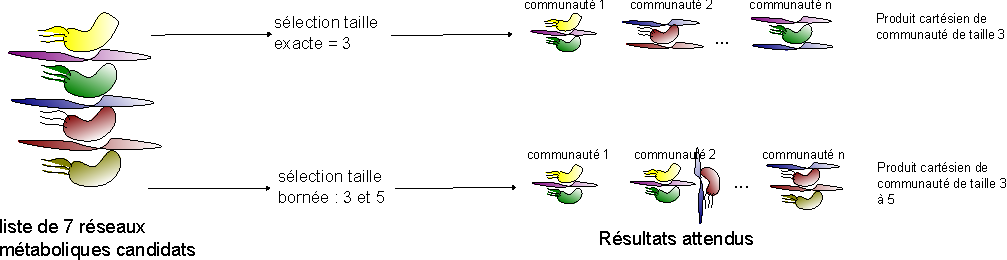
\includegraphics[scale=0.8]{img/enrichissement/figure_chapitre_renichissement.pdf} 
%    \caption{Exemple du principe de la sélection de communauté par sa taille.}
%    \label{fig:selection-taille}
%\end{figure}

Par exemple, un ou une biologiste aimerait obtenir l'ensemble des communautés qui ont une taille comprise entre \textbf{6} et \textbf{8}. Le fichier YAML d'entrée se structurerait ainsi:

\noindent
\begin{lstlisting}[style=yaml]
# Size constraints
SIZE:
  size: 
  lower bound: 6
  upper bound: 8
\end{lstlisting}

À partir de la lecture de ce fichier YAML, l'outil génère la liste de fait ASP, permettant de représenter les contraintes sous forme de connaissance:\\
\noindent
\begin{lstlisting}
lower_bound_size("6").
upper_bound_size("8").
\end{lstlisting}
 
Dans le cas où une taille fixe est demandée par les biologistes, seul le mot clé \texttt{size} est concerné. Par exemple, la demande "je ne veux que des communautés de taille \textbf{4}" se traduit par:
\begin{lstlisting}[style=yaml]
# Size constraints
SIZE:
  size: 4
  lower bound: 
  upper bound: 
\end{lstlisting}
Avec la \textbf{liste de faits ASP} suivante: \\
\begin{lstlisting}
lower_bound_size("4").
upper_bound_size("4").
\end{lstlisting}

Dans le cas où une taille fixe et une taille bornée sont renseignées, l'outil considère seulement la taille fixe.

\paragraph*{Contraintes sur la composition taxonomique bactérienne}
En plus de la taille, la ou le biologiste peut décider de la composition taxonomique, au grain de la souche, des communautés sélectionnées. Nous avons supposé que l'utilisateur ou l'utilisatrice connait un sous ensembles des souches bactériennes. Cette contrainte répond à des demandes biologiques telles que: "Au sein de ma communauté, je souhaite que les souches \textbf{XXX} et \textbf{YYL} soient présentes car elles permettent la libération de composés d'arômes d'intérêt, mais je ne veux surtout pas la souche \textbf{HHJ} et \textbf{KM} car elles sont en compétition avec les précédentes souches". Remarque, les raisons biologiques justifiants les intérêts pour ces souches ne sont pas prises en compte au sein de l'outil. Cette contrainte de présence absolue et d'interdiction se traduit respectivement dans le YAML part les clés d'entrée suivante: \texttt{always} et \texttt{forbid}:

\noindent
\begin{lstlisting}[style=yaml]
# Bacterial composition 
constraints
BACTERIAL COMPOSITION:
  always: 
    - XXX
    - YYL
  forbid: 
    - KM
    - HHJ
\end{lstlisting}

La liste de faits ASP à partir de ces contraintes sont les suivants:\\
\begin{lstlisting}
always("XXX").
always("YYL").
forbid("KM").
forbid("HHJ").
\end{lstlisting}


Nous avons également développé des contraintes supplémentaires sur la composition taxonomique de la communauté: associations interdites et obligatoires, nommées respectivement \texttt{forbidden asso} et \texttt{mandatory asso}. Une demande biologique illustrant ces propos serait: "S’il existe une communauté où une des souches \textbf{XV}, \textbf{FV} ou \textbf{JH} est présente, alors l'ensemble de ces souches doit être présent également. En revanche, tant que l'ensemble des souches \textbf{FV}, \textbf{PP} et \textbf{FT} n'est pas présent \underline{ensemble} dans la même communauté, mais que des sous-ensembles le sont, je considère la communauté valide." Ces contraintes diffèrent de \texttt{always} et de \texttt{forbid} du fait des notions d'ensemble, et l'ensemble nul est considéré comme valide du point de vue méthodologie: par exemple,  une communauté où ni \textbf{XV}, \textbf{FV} ou ni \textbf{JH} n'est présente, est valide. Ces associations permettent également de définir des différents groupes de souches interdites ou obligatoires. Par exemple, en complétant la demande: "En plus de ces associations, si une des souches \textbf{AA} et \textbf{ZS} est présente alors l'ensemble doit être présent également. Cependant, l'ensemble \textbf{PO} et \textbf{ML} ne doit pas être ensemble". Grâce au YAML, ces contraintes sont formalisables comme suit:


\noindent
\begin{lstlisting}[style=yaml]
# Bacterial composition 
constraints
BACTERIAL COMPOSITION:
forbidden asso: 
    - 
      - FV
      - PP
      - FT
    - 
      - PO
      - ML

  mandatory asso: 
    - 
      - XV
      - FV
      - JH
    - 
      - AA
      - ZS
\end{lstlisting}
Les différents groupes d'ensemble interdits (resp. obligatoires) sont symbolisé par \texttt{\_} de la ligne 5 et 9 (ligne 14 et 18). Ces groupes sont également visibles dans liste de faits ASP générée à partir de ces contraintes et se traduisent par le numéro en amont de la souche et sont définis automatiquement à la lecture du fichier YAML:\\

\noindent
\begin{minipage}[t]{0.45\textwidth}
\begin{lstlisting}
forbidden_asso("0","FV").
forbidden_asso("0","PP").
forbidden_asso("0","FT").
forbidden_asso("1","PO").
forbidden_asso("1","ML").
\end{lstlisting}
\end{minipage}% % leave no gap
\hspace{2em}\begin{minipage}[t]{0.5\textwidth}
\begin{lstlisting}
mandatory_asso("0","XV").
mandatory_asso("0","FV").
mandatory_asso("0","JH").
mandatory_asso("1","AA").
mandatory_asso("1","ZS").
\end{lstlisting}
\end{minipage}

\paragraph*{Flexibilité des fonctions objectives.}
Laisser le choix à l'utilisateur ou l'utilisatrice d'optimiser une ou plusieurs fonctions objectives correspond à l'enrichissement majeur du modèle logique. Comme nous avons vu précédemment, le choix de la fonction objective est important et sa modularité auprès de l'utilisateur ou l'utilisatrice l'est tout autant. Notre prototype d'outil prend actuellement les choix d'optimisation suivant: maximiser ou minimiser les échanges métaboliques, les métabolites cibles à produire, le scope métabolique et le nombre de substrats polyopsonistes. À partir du fichier d'initialisation YAML, les contraintes de maximisation ou de minimisation sont directement écrits ainsi:

\noindent
\begin{lstlisting}[style=yaml]
# Optimisation
OPTIMISATION: 
  - max
  - max

# Objectif
OBJ:
  - target
  - exchanged
\end{lstlisting}

Les lignes 3 et 4 indiquent le choix de l'optimisation que l'utilisateur ou l'utilisatrice souhaite faire, et les lignes 8 et 9 sont les objectifs possibles décrits plus haut. Dans cet exemple, le ou la biologiste veut en \underline{premier} maximiser la production d'un ensemble de cibles, puis, dans un \underline{second temps}, maximiser les métabolites échangeables. L'implémentation de cette contrainte se traduit de la façon suivante en ASP:\\

\begin{lstlisting}[label=lst:optimisation]
#maximize {1@1,M:target(M), pscope(M,_,_) }; 0@1}.
#maximize {1@2,S:exchanged(S); 0@2}.
\end{lstlisting}

Les priorités d'optimisation sont traduites par \texttt{1@1} et \texttt{1@2}, dans lequel la ligne 1 maximise le nombre de métabolites cibles présents dans le scope communautaire. \maxime{Adapter selon le nouveau formalisme développé dans CCMC ? ou mettre des noms plus communs pour aider la compréhension ?} 

\subsubsection*{Implémentation des nouvelles contraintes}
Nous venons de voir comment nous avons construit notre base de faits utiles pour formaliser les règles et les contraintes, conduisant à la sélection des communautés. Dans la suite de ce chapitre, nous allons formaliser les différentes règles et contraintes en ASP et expliciter formalisme mathématique. 

\paragraph*{Sélection par la taille de communauté}
Au sein du programme ASP, nous avons sélectionner les communautés par taille de la façon suivante:
\begin{lstlisting} [label=lst:taille]
lower_bound_size {chosen_bacteria(X):bacteria(X)} upper_bound_size.
\end{lstlisting}

Le listing \ref{lst:taille} sélectionne un sous ensemble de taille minimal \texttt{lower\_bound\_size.} et de taille maximal \texttt{upper\_bound\_size.} parmi l'ensemble \texttt{chosen\_bacteria(X)}, où X est dans le domaine défini par l'ensemble des bactéries (\texttt{bacteria}). Cela revient à sélectionner au hasard des bactéries (\texttt{chosen\_bacteria(X)}) parmi l'ensemble des bactéries initialement défini \texttt{bacteria}, où le nombre de bactéries sélectionner ne peut-être plus grand que \texttt{upper\_bound\_size.} et plus petit que \texttt{lower\_bound\_size.}\\

Mathématique, soit $t$ un sous-ensemble de taxon appartenant à l'ensemble de taxon \Ts, où un taxon correspond à une bactérie, la cardinalité $\vert t \vert $ doit être compris entre les valeurs $min$ et $max$:

\[
\forall t \in \Ts 
\]
\[
min<\vert t \vert <max
\]

\paragraph*{Sélection par la composition taxonomique au grain de la souche.}
Nous avons laissé la possibilité à l'utilisateur et à l'utilisatrice de filtrer sur la composition taxonomique de la communauté, avec les prédicats \texttt{always},\texttt{forbid},\texttt{mandatory\_asso} et \texttt{forbidden\_asso}.  

Le prédicat \texttt{always}, représentant un taxon qui doit être présent dans toutes les communautés possibles est implémenté en ASP comme suit:

\begin{lstlisting} [label=lst:always]
:- always(X); not chosen_bacteria(X).
\end{lstlisting}

Cette règle ne dispose pas de tête, on parle alors de contrainte d'intégrité. Elle se lit comme suit: parmi l'ensemble de bactérie initial, nous ne voulons pas les communautés où la bactérie définit par le prédicat \texttt{always(X)} n'est pas présente. La double négation étant lourde, nous pouvons traduire ainsi: sélectionne l'ensemble des communautés où la bactérie présumé \texttt{always} est présente. 

Mathématiquement, soit $A$ l'ensemble de bactéries obligatoirement présent dans la communauté:
\[
\forall t \in \Ts \text{ si } \forall A \in t 
\]

Concernant les bactéries qui ne doivent pas être présent dans la communauté, le code ASP ainsi que le formalisme mathématique est très ressemblant:

\begin{lstlisting} [label=lst:forbid]
:- chosen_bacteria(X); forbid(X) : chosen_bacteria(X).
\end{lstlisting}

Cela se traduit par: les communautés qui possèdent un ensemble de bactéries interdites (\texttt{forbid(X)}) parmi l'ensemble des bactéries tirées au sort ne doivent pas être sélectionnées. Mathématiquement, on appelle l'ensemble de bactérie interdit $F$, et est défini comme suit:

\[
\forall t \in \Ts \text{ si } \forall F \not \in t 
\]

Nous avons également défini des associations obligatoires (\texttt{mandatory\_asso}) et interdites (\texttt{forbidden\_asso}). Pour rappel, l'utilisateur ou l'utilisatrice pouvait définir des groupes d'association, nommé \texttt{group\_forbidden(G)} dans le cas des associations interdites. Ce prédicat regroupe l'ensemble des groupes (\texttt{G}) que la ou le biologiste a défini dans le fichier de configuration YAML. Nous avons défini les associations obligatoires en 3 parties.

Dans le listing \ref{mandatory1}, les communautés sélectionnées (\texttt{selected\_bacteria(X)}) ont obligatoirement toutes les bactéries de l'ensemble des associations obligatoires parmi l'ensemble de bactéries préalablement choisis (\texttt{chosen\_bacteria(X1) : mandatory\_asso(\_,X1).}).

\begin{lstlisting} [label=mandatory1,caption=Règle numéro 1 pour définir les associations obligatoires, captionpos=b]
selected_bacteria(X) :- chosen_bacteria(X); 
		  chosen_bacteria(X1) : mandatory_asso(_,X1).
\end{lstlisting}

Il faut ensuite rajouter les communautés où aucune des bactéries des associations obligatoires n'est présent parmi l'ensemble de bactéries préalablement défini (\texttt{not chosen\_bacteria(X1) : mandatory\_asso(\_,X1).}). Ce calcul est illustré par le code dans le llisting \ref{mandatory2}

\begin{lstlisting} [label=mandatory2,caption=Règle numéro 2 pour définir les associations obligatoires, captionpos=b]
selected_bacteria(X) :- chosen_bacteria(X);
	    not chosen_bacteria(X1) : mandatory_asso(_,X1).
\end{lstlisting}

Enfin, pour une question de visualisation des solutions, nous avons ajouté la contrainte d'intégrité \ref{mandatory3} qui ne montre que les communautés filtrées par les associations obligatoires.

\begin{lstlisting} [label=mandatory3,caption=Règle numéro 3 pour définir les associations obligatoires, captionpos=b]
:- chosen_bacteria(X); not selected_bacteria(X).
\end{lstlisting}

Mathématiquement, soit $O$ l'ensemble des bactéries des associations obligatoires, et $o_i \forall i \in O$. Les associations obligatoires sont définies comme:

\[
\forall O \in \Ts \text{ si } o_i = t \text{ alors } \forall o_i \in t 
\]

Enfin, pour définir les associations interdites au sein d'une communauté (voir listing \ref{lst:forbidden}, les communautés sélectionnées ne doivent pas posséder l'ensemble des bactéries interdites parmi les communautés déjà sélectionnées (\texttt{chosen\_bacteria(X2) : forbidden\_asso(G,X2).})

\begin{lstlisting} [label=lst:forbidden, caption=Règle définissant les associations interdites, captionpos=b]
:- chosen_bacteria(X); group_forbidden(G);
		chosen_bacteria(X2) : forbidden_asso(G,X2).
\end{lstlisting}

Mathématiquement, soit $I$ l'ensemble des bactéries des associations interdites et $I_i \forall i \in I$. Les associations interdites sont alors définies comme:

\[
\forall I \in \Ts \text{ si } \forall I_i \not \in t \text{ alors } I_i \in t 
\]

\begin{figure}[h!]
    \centering
    \includegraphics{example-image-a}
    \caption{Montrer en image le workflow complet en illustration. Montrer la facilité d'utilisation pour les biologistes et les liens entre chaque modification faite par l'utilisateur et la contrainte formalisés.}
    \label{fig:my_label}
\end{figure}
\newpage

\subsection{Résultats préliminaires}
Nous venons de décrire et détailler la base de connaissance nécessaire pour sélectionner des communautés à façon. Dans cette sous-section, nous allons dans un premier temps identifier des questions biologiques provenant d'un retour d'expérience sur les précédents chapitres ainsi que de discussions avec les biologistes, et comment l'outil de sélection permet d'y répondre. Puis dans un second temps, nous allons appliquer notre méthode de sélection de communauté à façon sur le jeu de données du papier M2M \citep{Belcour.2020} afin de montrer son efficacité à passer à l'échelle.

\subsubsection*{Exemples}
Toutes les questions ci-dessous vont chercher à identifier des ensembles de communautés candidates pour des objectifs métaboliques supposés connus. Les questions seront présentées des plus larges au plus précises. Nous utiliserons les réseaux métaboliques reconstruits à l'échelle du génome de Weiss \citep{Weiss2022}. Ils ont été reconstruits avec l'outil GapSeq\citep{Zimmermann2021} et un consortium bactérien permettant une analyse des interactions métabolique de l'intestin de souris a été créé.


\paragraph*{\textit{Pour une communauté de taille 5, existe-t-il une communauté qui métaboliste l'ensemble des acides aminés?}}
Cette question nous permet d'identifier les deux contraintes à utiliser au sein de l'outil: la liste des composés que l'on doit produire, \textit{i.e.} les acides aminés (AA), ainsi que la taille de la communauté finale, \textit{i.e.} 5. 

Le fichier initial est donc constitué des informations suivantes:
\begin{lstlisting}[style=yaml]
# Size constraints
SIZE:
  size: 5
\end{lstlisting}

N'ayant précisé aucune optimisation, l'ensemble des cibles, que sont les acides aminés, devront être dans le scope de la communauté. Le résultat pour cette situation est \textbf{unsatisfiable}. Cela signifie qu’il n’existe pas de modèles permettant de satisfaire les contraintes de l'utilisateur ou de l'utilisatrice, et donc aucune communauté de taille n'a été trouvé comme étant capable de métaboliser l'ensemble des acides aminés.
Le premier réflexe de l'utilisateur ou de l'utilisatrice est de formuler la demande de façon à relâcher les contraintes. La contrainte la plus forte ici consiste à obtenir au moins une communauté permettant de l'ensemble des \textbf{métaboliser les acides aminés}. Une reformulation possible serait: métaboliser un \textbf{maximum} d'acide aminé. En appliquant cette modification nous obtenons une communauté composée des souches \textit{I48}, \textit{KB1m}, \textit{YL44}, \textit{YL45}, \textit{YL27}.\\

\paragraph*{\textit{Pour une communauté composée de 6 taxa, laquelle permet la plus grande production métabolique sans les échanges métaboliques?}} 
Nous avons 2 types de contraintes: 2 optimisations, que sont la maximisation du scope communautaire et la minimisation des échanges métaboliques, et taille, et se traduit comme suit dans le fichier d'initialisation:

\begin{lstlisting}[style=yaml]
# Size constraints
SIZE:
  size: 5
  
  # Optimisation
OPTIMISATION: 
  - max
  - min

# Objectif
OBJ:
  - scope
  - exchanged
\end{lstlisting}

La meilleure communauté, selon le solveur, possède 797 échanges et 1010 métabolites sont productibles en communauté. En plus de connaître la meilleur composition taxonomique répondant à ces contraintes, le vocabulaire contrôlé développé dans le chapitre \ref{ccmc} est également accessible: les métabolites échangeables, les consommateurs et producteurs intervenant dans l'échange, les substrats polyopsonistes, les potentiels de coopération et de compétition.



\paragraph*{\textit{A partir d'une communauté de 150 réseaux métaboliques de l'intestin, j'aimerai une étudier une communauté de composé de 6 à 8 taxons garantissant une productibilité d'un maximum des 23 composés d'intérêts}}
En plus de ces contraintes, il y a des contraintes de composition taxonomique que sont: \textit{les réseaux métaboliques GCA\_003433685, GCA\_003433675 et GCA\_003433665 doivent-être \underline{présent}, GCA\_003433745, GCA\_003433755 et GCA\_003433765 doivent \underline{jamais apparaître} dans la ou les communautés. Les ensembles GCA\_003433795, GCA\_003433825 et GCA\_003433845 \underline{ou} GCA\_003433855 et GCA\_003433865 ne doivent pas être présents. En revanche, les ensembles GCA\_003433905, GCA\_003433925 et GCA\_003433945 \underline{ou} GCA\_003433955 et GCA\_003433985 doivent être présent.} Cette demande factice test le passage à l'échelle de la méthode. Nous avons donc utilisé 150 réseaux métaboliques reconstruits dans le chapitre \ref{ccmc} :\\

\noindent
\begin{minipage}[t]{0.4\textwidth}
\textbf{contrainte d'entrée}: 
\begin{lstlisting}[style=yaml]
# Size constraints
SIZE:
  size: 
  lower bound: 6
  upper bound: 8

# Bacterial composition
 constraints
BACTERIAL COMPOSITION:
  in: 
    - GCA_003433685
    - GCA_003433675
    - GCA_003433665
  out: 
    - GCA_003433745
    - GCA_003433755
    - GCA_003433765
  forbidden asso: 
    - 
      - GCA_003433795
      - GCA_003433825
      - GCA_003433845
    - 
      - GCA_003433855
      - GCA_003433865

  mandatory asso: 
    - 
      - GCA_003433905
      - GCA_003433925
      - GCA_003433945
    - 
      - GCA_003433955
      - GCA_003433985
      
# Optimisation
OPTIMISATION: 
  - max

# Objectif
OBJ:
  - target
\end{lstlisting}
\end{minipage}% % leave no gap
\hspace{2.5em}\begin{minipage}[t]{0.5\textwidth}
\textbf{sortie}: 

\begin{lstlisting}
Answer: 1

GCA_003433925.
GCA_003433985.
GCA_003433685.
GCA_003433675.
GCA_00343390.
GCA_003433945.
GCA_003433665.
GCA_003433955.
\end{lstlisting}
\textbf{Performance}: 

Models: 1

Time: 197.120s 

CPU Time: 196.781s\\

En maximisant une liste de composés d'intérêt (23) et à partir des paramètres ci-dessus, nous avons trouvé une communauté candidate en environ 3 minutes et 30 secondes.
\end{minipage}

\section{Discussion et conclusion}
Cette première exploration d'enrichissement d'un modèle logique a répondu aux remarques majeures que nous avons énoncées plus haut: filtrer le nombre de solutions d'un modèle logique et optimisation de fonctions objectives. En effet, l'outil développé dans le chapitre \ref{ccmc} permet de donner une indication des potentiels de coopération et de compétition de communautés microbiennes mais ne permet pas d'identifier les critères permettant de l'affirmer. Avec ce prototype, nous avons proposé un moyen de sélectionner la meilleure communauté selon les critères de l'utilisateur ou de l'utilisatrice, et par extension, de définir la communauté avec un fort potentiel de coopération ou de compétition. Cela a été possible en ajoutant une optimisation d'une ou de plusieurs fonctions objectives. La plus-value par rapport au logiciel MISCOTO est que l'utilisateur ou l'utilisatrice choisi la fonction objective qu'il ou elle souhaite optimiser.\\

Cependant, aucune validation expérimentale n'a été faite à ce jour. Au regard de la littérature concernant la création de communauté à façon, une validation expérimentale est nécessaire pour créer une bonne communauté synthétique \citep{Sharma2020,Vazquez-Castellanos2019}. Par exemple, Macchi et ses collègues \citep{Macchi2021} ont construit une communauté bactérienne à partir de 6 génomes isolés pour la dégradation du phénanthrène. \\

Vis à vis des interactions bactériennes, ce prototype permet de se concentrer essentiellement sur le potentiel de coopération d'une communauté bactérienne. Concernant le potentiel de compétition uniquement défini par les substrats polyopsonistes, c'est à dire un nutriment qui est co-consommé, l'ajouté de la temporalité semble être un bon moyen pour améliorer la prédiction de la compétition. En effet, dans le chapitre \ref{tango}, le lactose est bien co-consommé mais pas au même moment dans le temps, empêchant de définir un lien de compétition pour ce substrat. Afin d'essayer de prendre en compte une pseudo-temporalité au sein des modèles logiques, nous allons utiliser la logique temporelle de Cabalar \citep{Cabalar2019}.


\newpage

\section{Intégration d'une temporalité réactionnelle}
La logique linéaire temporelle (LTL), à notre connaissance, n'a jamais été appliquée dans un contexte biologique. Pourtant, dans son domaine d'application IA, l'inférence de règles temporelles permet d'affiner les prédictions en proposant des explications séquentielles. Brièvement, Cabalar se base sur le problème de raisonnement sur les actions et le changement (RAC). Il en existe 5: (i) la \textbf{simulation}; étant donné un état initial du système et une suite d'actions, la simulation permet de prédire l'état du système à un temps futur. (ii) L'\textbf{explication}; étant donné un état initial et un état futur du système, l'explication propose une séquence d'état intermédiaires du système menant de l'état initial à l'état final. (iii) \textbf{Planification}; étant donné un état initial du système et un objectif, la planification propose une séquence d'actions, éventuellement non-déterministes, garantissant l'objectif. (iv) \textbf{Diagnostique}; à partir d'une définition de transitions d'état normal et anormal ainsi qu'un ensemble d'états observés (normal et anormal),  le diagnostique propose un ensemble minimal de transitions expliquant les observations anormales. (v) \textbf{Vérification}, validation d'une propriété temporelle du système (comme sûreté, vivacité ou équité) ou une propriété de représentations (comme l'équivalence de modèles). \\

Le premier défi est l'application de ces concepts RAC à la biologie des systèmes. Nous avons donc associé le système à une communauté de GEMs et les actions à des activations de réactions. Ainsi, chaque nouvelle activation d'une réaction, selon l'algorithme d'expansion du réseaux métabolique d'Ebenhöh, consistera un nouvel état du système. En prenant un exemple simple de la communauté fromagère du chapitre \ref{tango}, nous savons que le propionate est produit à partir du lactate. Remarquons ici que nous ne précisons pas les organismes pour le moment. À partir de cette information nous pouvons déduire \textit{a minima} une relation de dépendance logique temporelle, qui est: pour qu'\textit{a un moment de la cinétique de fermentation} le propionate soit productible, il faut que le lactate soit productible \textit{avant}. En appliquant la LTL à des réseaux métaboliques, les notions temporelles \textit{un moment} et \textit{avant} seront définies selon la longueur du chemin menant à la production du composé: propionate. Au sein de la LTL, le solveur,  \textit{telingo}, cherche à minimiser la taille du chemin. Ainsi, à partir d'un ensemble de nutriments disponibles dans le milieu extracellulaire, un ensemble fini de voies métaboliques mène à la production d'un composé cible, et \textit{ \textit{ \textit{telingo}}} priorise le chemin le plus court, c'est à dire le nombre réaction le plus faible. De ce fait, la temporalité n'est pas représentée comme une dimension, tel que présent dans le dFBA par exemple, mais par une séquence d'actions, activation ou non d'une réaction: on parle de \textit{temporalité réactionnelle}. Dans la suite de ce chapitre nous allons définir les cas d'utilisation de Cabalar et les appliquer à la communauté du chapitre \ref{tango}.


\subsubsection*{Inférence temporelle dans la programmation logique}

\paragraph*{Solveur \textit{ \textit{ \textit{telingo}}}}
Nous avons vu que les modèles numériques, contrairement aux modèles logiques, pouvaient intégrer une dimension temporelle et ainsi analyser d'autres propriétés du système biologique. Il existe un formalisme informatique, nommé \textit{logique temporelle linéaire} ou LTL, qui permet d'introduire une notion de temporalité au sein des modèles logiques. 

Ce modèle de logique par raisonnement se base sur le même formalisme que celui décrit dans le chapitre \ref{ccmc}: une base de faits, des règles et contraintes doivent-être générées. \textit{telingo}permet d'intégrer des contraintes temporelles et les règles et contraintes utilise les opérateurs logiques temporels décrits dans la Figure \ref{fig:syntaxe}.

 \begin{figure}[h!]
	\centering
    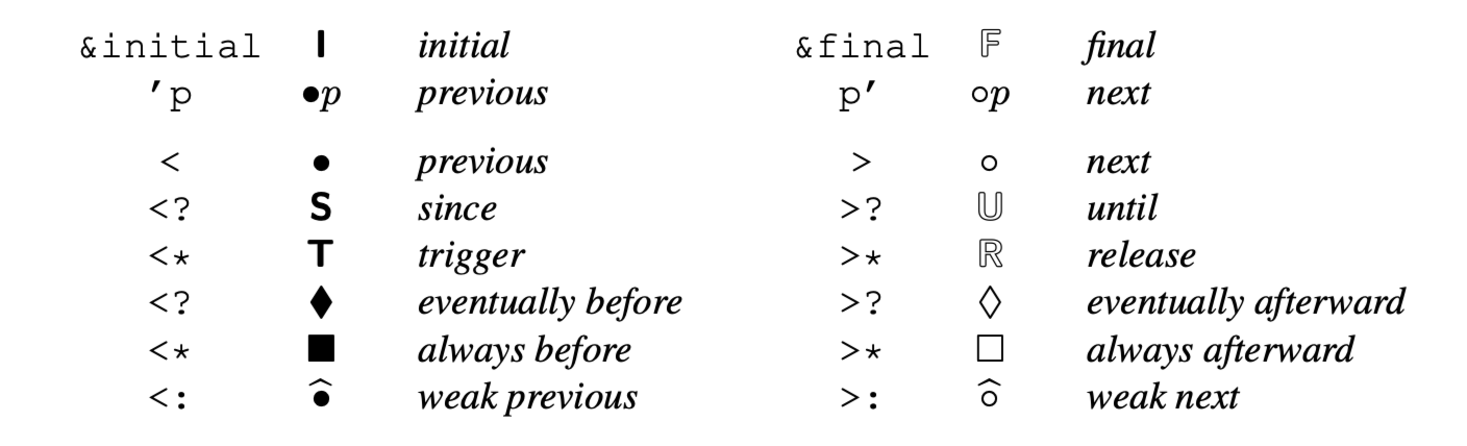
\includegraphics[width=\textwidth]{img/enrichissement/syntaxe_telingo}
    \caption{Opérateurs temporels du futur et du passé en \textit{telingo}et logique temporelle issue de \citep{Cabalar2019}}
    \label{fig:syntaxe}
\end{figure}

Dans l'exemple ci-dessous, nous avons défini une proposition vraie tout le temps : Quelque chose est \textit{chargé} si \textbf{au temps précédent} il a été \textit{chargé} et qu'il n'est pas \textit{déchargé}.  

\begin{lstlisting}[mathescape=True]
    charge :- $\square$ ($\bullet$ charge; not decharge)
\end{lstlisting}

À partir de cette nouvelle synthaxe, nous avons créé une communauté jouet du chapitre \ref{tango} afin d'appliquer la LTL et d'illustrer la temporalité réactionnelle au moyen de 3 concepts RAC: \textbf{planification}, \textbf{vérification} et \textbf{explication}. 

\subsection{Démarche à suivre}
Ce formalisme logique est une extension du formalisme décrit dans le chapitre \ref{ccmc} mais n'ayant jamais été appliqué sur des réseaux métaboliques, nous avons représenté les réseaux métaboliques de \freud, \plantarum et \lactis de manière simplifiée et minimaliste. Ce choix méthodologique a été imposé pour deux raisons: éviter dans un premier temps la problématique du passage à l'échelle et dans un second temps, permettre de résoudre les défis rencontrés lors de l'application des concepts de Cabalar. Dans les sous-sections qui suivent, nous présenterons les différents cas d'utilisation de Cabalar ainsi que leur résolution à partir d'une communauté factice, puis, l'application de ces concepts sur les réseaux métaboliques du chapitre \ref{tango}.

\subsection{Explication des concepts de Cabalar}

\subsubsection*{Ensemble de règles en \textit{telingo}pour la modélisation d'une communauté de bactéries}

\paragraph*{Scope}
Nous avons redéfini le vocabulaire exprimé dans le chapitre \ref{ccmc} en intégrant le vocabulaire temporel de la LTL. Ainsi, les notions de réactions activées et de composés productibles deviennent:

\begin{lstlisting}[label = lst:isActivated, caption = Règle d'activation d'une réaction, captionpos=b ]
0{isActivated(Rea,Org)}1 :- product(Compound,Rea,Org,_) ;
'producible(Reactant,Org) : reactant(Reactant,Rea,Org,_).
\end{lstlisting}

\begin{lstlisting}[label=lst:productible, caption = Règle de productibilité d'un composé, captionpos=b]
producible(Compound,Org):-  product(Compound,Rea,Org,_),
isActivated(Rea,Org).
\end{lstlisting}

Les contraintes exprimées dans les listings \ref{lst:isActivated} et \ref{lst:producible} signifient qu'une réaction est activée si l'ensemble des réactants ont été produits \textit{avant} (représenté par l'apostrophe \texttt{'}). Un composé est considéré comme productible si c'est un produit d'une réaction et qu'elle est activée.

L'évolution de la concentration d'un métabolite au cours du temps n'étant pas inférée dans le modèle, nous ne pouvons déterminer quand une réaction n'est plus activée. Nous assumons alors que si une réaction est activée une fois elle ne peut l'être une seconde fois. Cette règle s'exprime sous la proposition logique suivante :

\begin{lstlisting}[label=lst:notactivated, caption = Règle interdisant qu'une réaction soit activée deux fois, captionpos=b]
not isActivated(Rea,Org) :- not not &tel{ <? isActivated(Rea,Org)},
 reaction(Rea,Org).
\end{lstlisting}

% En revanche, déterminer quand est-ce qu'un métabolite devient polyopsoniste est possible. Ainsi, en utilisant le formalisme logique, une réaction n'est pas activée si celle-ci a déjà été activée dans le passé.

\paragraph*{Disponibilité des nutriments nouvellement productibles}
Avec cette notion temporelle à l'échelle d'une réaction, un composé produit en amont doit-être disponible pour une réaction qui se situerait en aval. La Figure \ref{disponible} illustre ce concept que nous avons développé. A partir du composé extracellulaire \texttt{Ae}, le composé C est productible au temps réactionnel 2. Il est ainsi disponible pour la réaction situé 2 temps réactionnel en aval, la réaction R4. 

    \begin{figure}[H]
        \begin{center}
            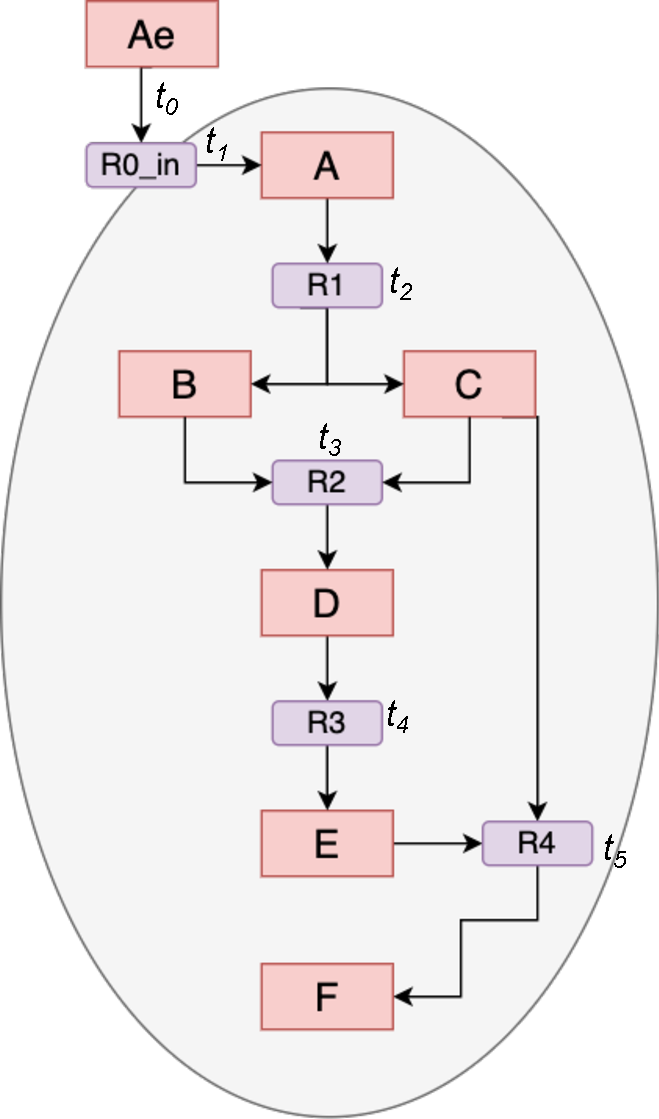
\includegraphics[scale=0.50]{img/enrichissement/reutilisation.pdf}
                \caption{Réutilisation du composé C par la réaction R4 où C était productible 2 étapes avant }
            \label{disponible}
        \end{center}
    \end{figure}
    
Avec cette nouvelle propriété, la définition de réaction activée est redéfinie ainsi: Une réaction est activée si tous les réactants de la réaction ont été productible avant (représenté par l'apostrophe à ligne 2):

\begin{lstlisting}
disponible(Compound,Org) :- producible(Compound,Org).
disponible(Compound,Org) :- 'disponible(Compound,Org).
\end{lstlisting} 

Bien entendu, au sein d'une communauté bactérienne, nous observons des échanges métaboliques. Les métabolites échangés ont été considérés comme productibles ils deviennent alors disponibles pour l'ensemble des membres de la communauté.

\subsection{Application de \textit{telingo} sur des organismes jouets}
Nous venons de voir les règles essentielles permettant de modéliser une communauté bactérienne avec la synthaxe temporelle. Dans les sections suivantes nous verrons l'applications du formalisme \textit{telingo} sur le des communautés jouets afin de vérifier si les concepts RAC s'adaptent bien sûr à la biologie des systèmes. Les règles et les contraintes utilisées pour modéliser les concepts RAC ne seront pas expliquées, seul l'aspect temporel sera mis en avant.

\subsubsection*{Planification}
Nous avons dès à présent les éléments nécessaires pour modéliser les cas d'application de Cabalar. Pour cela nous avons utilisé les réseaux métaboliques illustré par les Figures \ref{fig:planification} et \ref{fig:explication}. Dans le cas de la planification, l'objectif à atteindre était de déterminer la communauté minimale pour la production du composé Ne. Dans la figure \ref{fig:planification}, ce composé peut être produit soit par l'organisme 1 seulement et par l'organisme 2 par l'intermédiaire de 2 échanges métaboliques. La sortie du modèle est indiquée par le chemin en vert validant ainsi la prédiction.

\begin{figure}[H]
    \begin{center}
        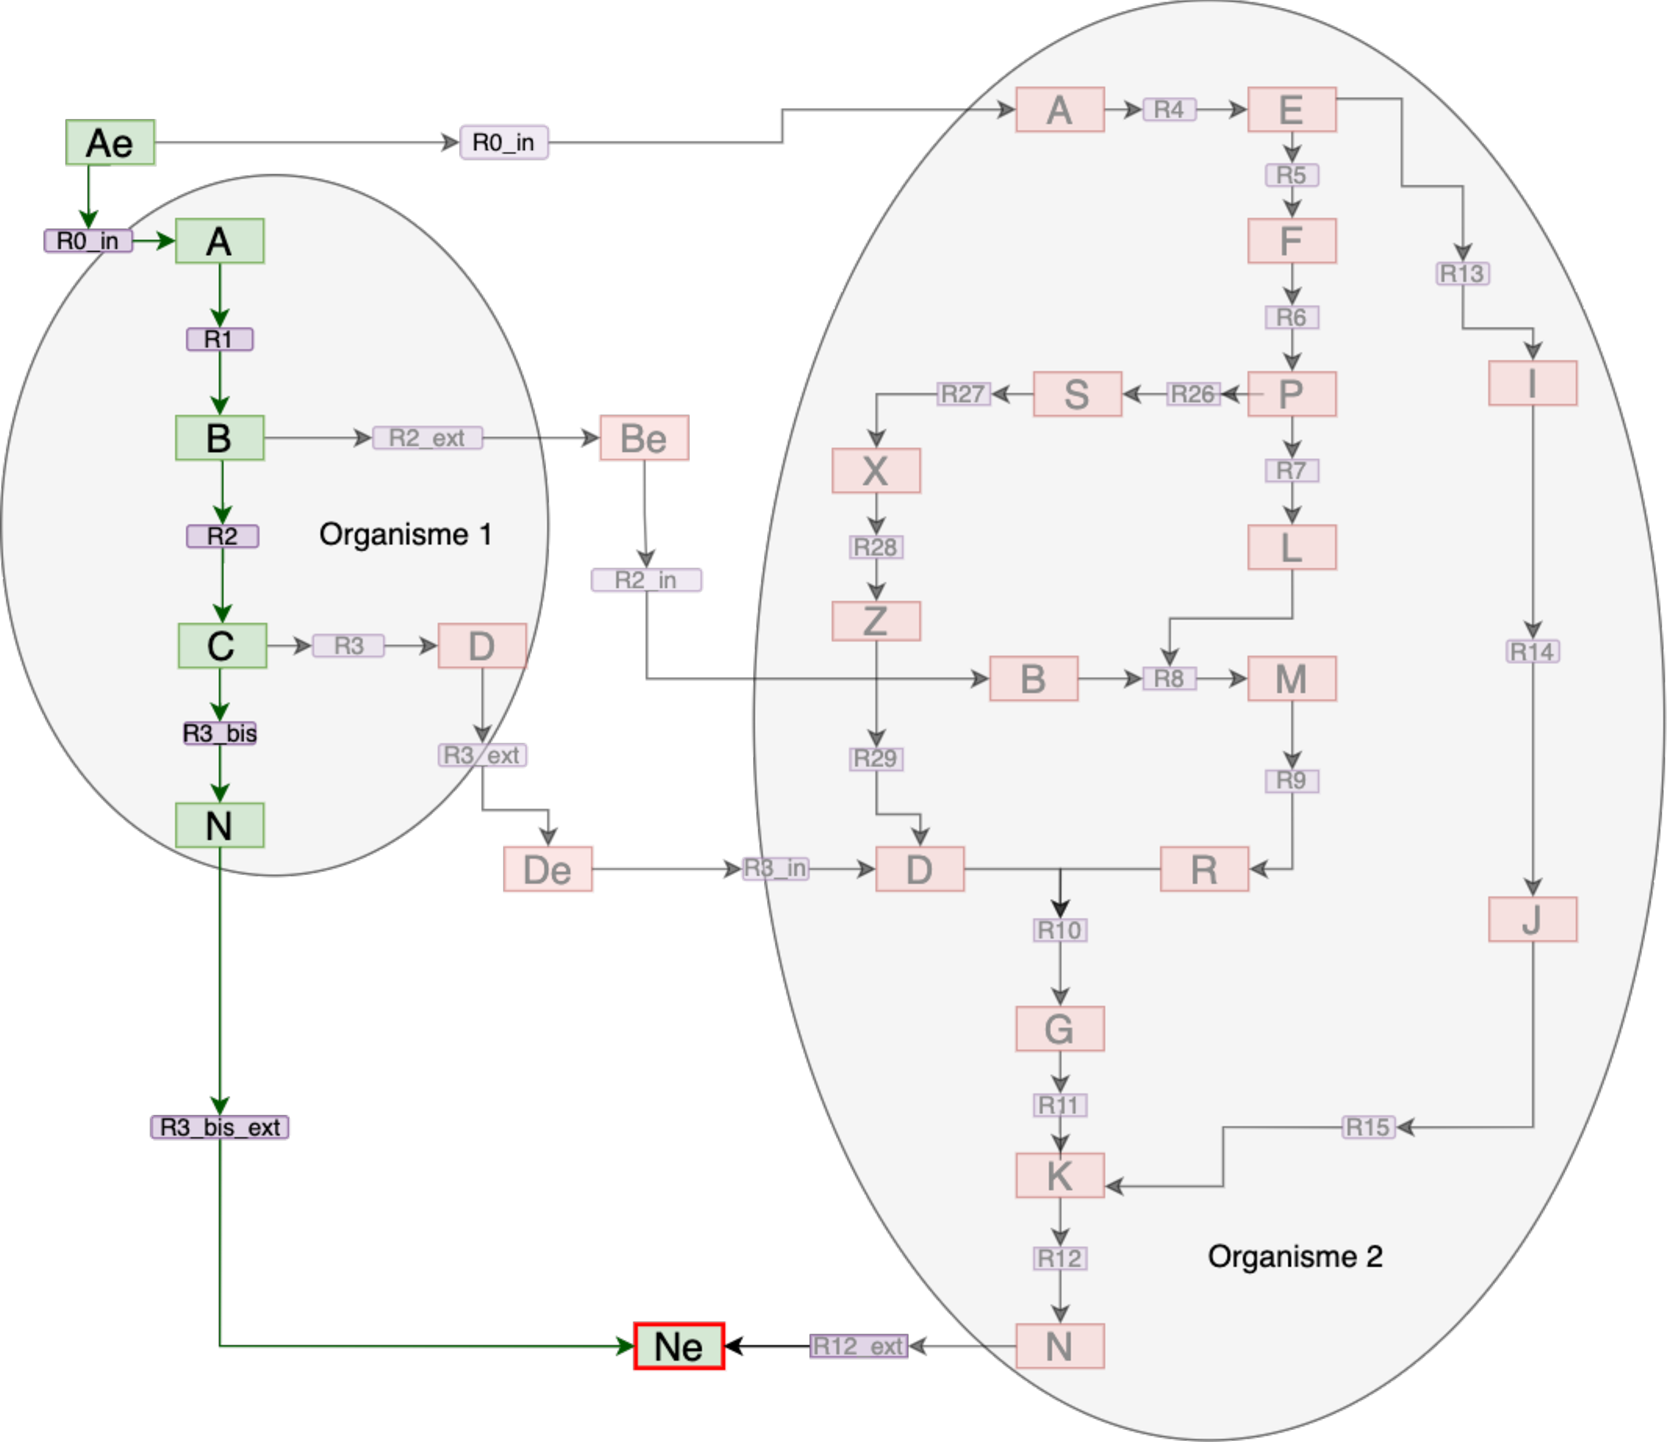
\includegraphics[scale=0.5]{img/enrichissement/Planification.pdf}
            \caption{Schéma didactique permettant de valider la solution donnée par le modèle dans le cas de la planification en montrant que le composé Ne est productible à partir d'un seul organisme via le chemin vert.}
        \label{fig:planification}
    \end{center}
\end{figure}

Aucune règle stipulant qu'une communauté est minimum composé de 2 taxons, \textit{telingo} montre que seul l'organisme 1 peut produire le composé \texttt{Ne}, comme indiqué par le listing \ref{lst:planification_res}.

\begin{lstlisting}[label =lst:planification_res, caption =Résultat de la planification obtenue après application des règles sur la base de faits, captionpos=b]
Answer: 1
 State 0:
 State 1:
  isActivated("R0_in","Org1")
  producible("A","Org1")
 State 2:
  isActivated("R1","Org1")
  producible("B","Org1")
 State 3:
  isActivated("R2","Org1")
  producible("C","Org1")
 State 4:
  isActivated("R3_bis","Org1")
  producible("N","Org1")
 State 5:
  isActivated("R3_bis_ext","Org1")
  producible("Ne","Org1")
Optimization: 1 5
OPTIMUM FOUND

Models       : 1
  Optimum    : yes
Optimization : 1 5
Calls        : 6
Time         : 0.265s (Solving: 0.00s 1st Model: 0.00s Unsat: 0.00s)
CPU Time     : 0.197s
\end{lstlisting}

Les séquences des actions montrant la production de \texttt{Ne} est représenté par “\texttt{State}" dans la sortie du modèle. Ici, Au temps réactionnel 0, aucune réaction est activée. Seul le composé extracellulaire \texttt{Ae} serait marqué comme étant \texttt{disponible}. Au temps réactionnel suivant, \texttt{State 1}, la réaction important le composé \texttt{Ae} dans le milieu intracellulaire est activé par la réaction \texttt{R0\_in} (voir ligne 4 du listing), et le composé \texttt{A} est \texttt{productible} et \texttt{disponible} (ligne 5). Au temps réactionnel suivant, \texttt{B} est \texttt{productible} et la réaction \texttt{R1} est activée. En procédant ainsi, Le composé \texttt{Ne} est \texttt{productible} et \texttt{disponible} pour l'ensemble de la communauté en 5 étapes, correspondant au temps réactionnel 5.


\subsubsection*{Vérification}
Le cas de vérification consiste simplement à vérifier qu'il existe une séquence de réactions activables permettant de produire un composé. Ainsi, nous avons vérifié la productibilité du composé \texttt{Ne}(voir listing \ref{lst:planification_res}):

Nous pouvons voir qu'à chaque pas de temps, marqué par "\texttt{State}", il existe au moins une réaction qui est activée, permettant à terme, de produire le composé \texttt{Ne}.


\subsubsection*{Explication}
Dans le cas de l'explication, nous cherchons à déterminer le chemin réactionnel permettant la production d'un composé sachant que l'on a observé la production d'un autre composé à un moment dans le temps. Brièvement, l'objectif est de savoir s’il existe une relation entre une observation faite à un moment dans le temps et l'objectif final. Dans le cas de notre exemple de l'explication représenté par la Figure \ref{fig:explication}, nous avons cherché à expliquer la production du composé \texttt{Ne} sachant que le composé \texttt{De} a été observé. Le résultat du modèle est indiqué par le tracé en vert. Le résultat du modèle est indiqué par le listing \ref{explication}:

\begin{lstlisting}[label=explication, caption=Résultat de l'explication obtenue après application des règles sur la base de faits didactique, captionpos=b]
 State 0:
 State 1:
  isActivated("R0_in","Org1") isActivated("R0_in","Org2")
  producible("A","Org1") producible("A","Org2")
 State 2:
  isActivated("R1","Org1") isActivated("R4","Org2")
  producible("B","Org1") producible("E","Org2")
 State 3:
  isActivated("R2","Org1") isActivated("R2_ext","Org1") isActivated("R5","Org2")
  producible("Be","Org1") producible("C","Org1") producible("F","Org2")
 State 4:
  isActivated("R2_in","Org2") isActivated("R3","Org1") isActivated("R6","Org2")
  producible("B","Org2") producible("D","Org1") producible("P","Org2")
 State 5:
  isActivated("R7","Org2")
  producible("L","Org2")
 State 6:
  isActivated("R3_ext","Org1") isActivated("R8","Org2")
  producible("De","Org1") producible("M","Org2")
 State 7:
  isActivated("R3_in","Org2") isActivated("R9","Org2")
  prod_explain("D","Org2")
  producible("D","Org2") producible("R","Org2")
 State 8:
  isActivated("R10","Org2")
  prod_activate("G","Org2")
  prod_activate_cof("G","Org2")
  producible("G","Org2")
 State 9:
  isActivated("R11","Org2")
  prod_activate("K","Org2")
  prod_activate_cof("K","Org2")
  producible("K","Org2")
 State 10:
  isActivated("R12","Org2")
  prod_activate("N","Org2")
  prod_activate_cof("N","Org2")
  producible("N","Org2")
Optimization: 3 17
OPTIMUM FOUND
Models       : 4
  Optimum    : yes
Optimization : 3 17
Calls        : 11
Time         : 0.366s (Solving: 0.02s 1st Model: 0.00s Unsat: 0.00s)
CPU Time     : 0.350s

\end{lstlisting}
Au temps réactionnel 6 (ligne 19), nous voyons que l'observation est expliquée, et qu'il faut attendre le temps réactionnel 10 pour que le composé final \texttt{Ne} soit productible. Nous pouvons également remarquer que le modèle explique en même temps la production du composé \texttt{Be} pour permettre la production de \texttt{Ne}: on dit alors que \texttt{Be} est un métabolite essentiel à la production de \texttt{Ne}.

\begin{figure}[H]
    \begin{center}
        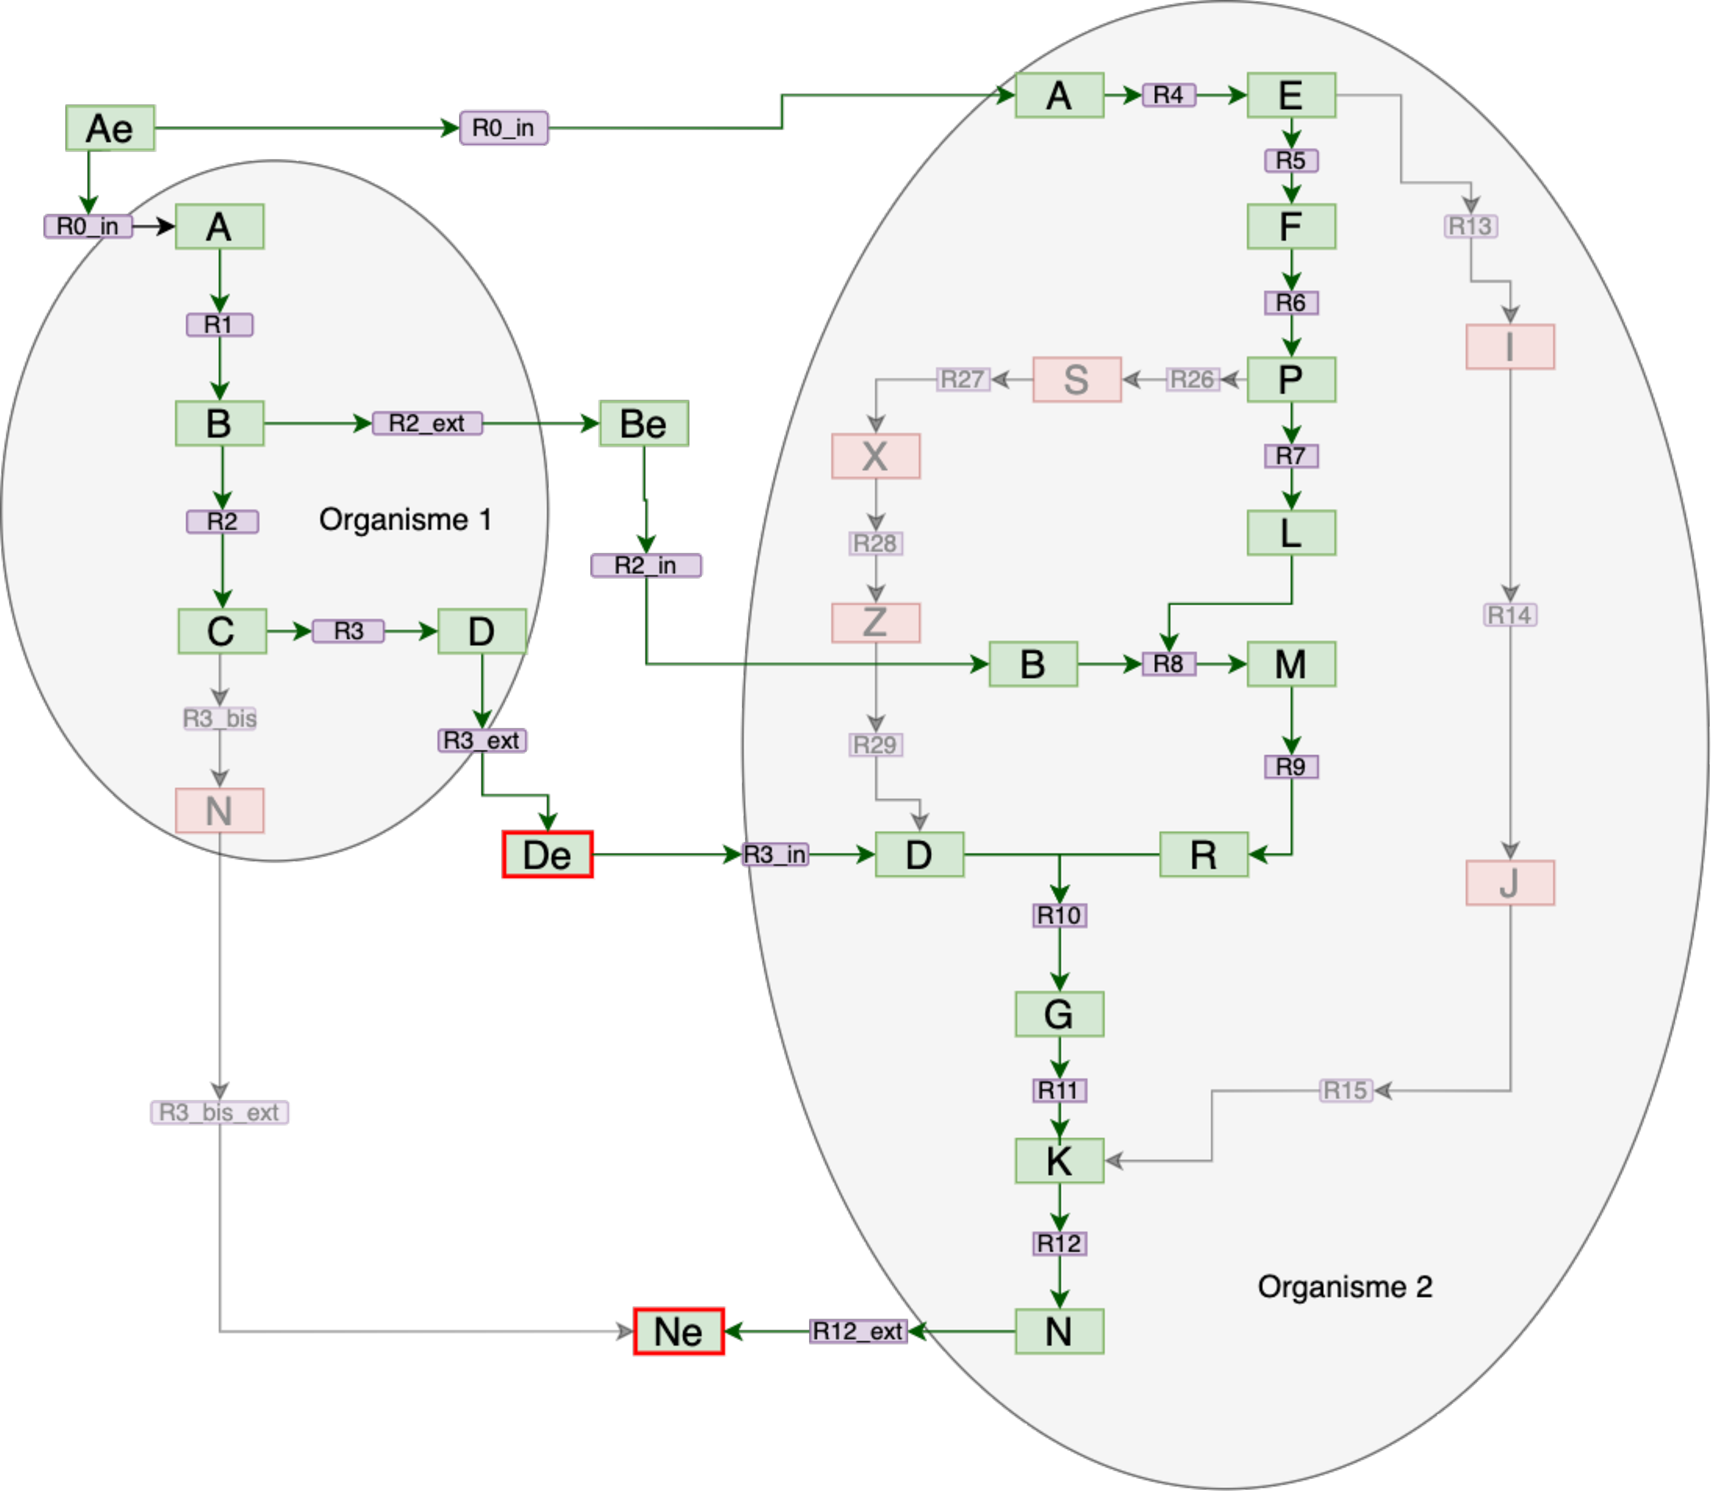
\includegraphics[scale=0.5]{img/enrichissement/Explication.pdf}
            \caption{Schéma didactique permettant de valider la solution donnée par le modèle dans le cas de l'explication en montrant que le composé Ne est productible à partir de l'élément observable De.}
        \label{fig:explication}
    \end{center}
\end{figure}
    
    
Cette implémentation temporelle, sur un schéma didactique, met en avant deux points intéressants par rapport à un dFBA. Le premier est la possibilité d'avoir la suite réactionnelle conduisant à un ou plusieurs objectifs finaux de façon direct. Cette représentation en temps réactionnel, permet donc de générer des hypothèses testables sur l'activation de ou non de voies métaboliques d'intérêt à travers des méthodes de knockout enzymatique par exemple. La seconde est la mise en avant indirect d'une coopération entre ces deux organismes. Pour rappel, la connaissance initiale montrait une observation dans le milieu extracellulaire de \texttt{De} et non un échange entre ces deux organismes. De plus, ce modèle a permis de montrer qu'un autre composé est échangé pour permettre de réaliser l'objectif final.
    
    
\section{Application à une communauté simplifié du chapitre \ref{tango}}
Nous avons repris le milieu du lait ainsi que les réseaux métaboliques du chapitre \ref{tango}, et généré la nouvelle base de faits applicable à \textit{telingo}. Nous présenterons que 2 cas: planification et explication.  \\

\subsection{Cas de la planification}
Dans le cas de la planification, le système initial est composé des 3 bactéries, du milieu nutritionnel du lait. L'objectif à attendre est la production de propionate, note \texttt{M\_ppa\_e} dans la sortie du modèle représenté par \ref{lst:planification_reel}:

\begin{lstlisting}[label = lst:planification_reel , caption = Résultat de la planification obtenue après application des règles sur la base de faits issue des données réelles]
 State 0:
 State 1:
  isActivated("R_ADK1_rev","lactis") isActivated("R_ARGDr","lactis")
  producible("M_amp_c","lactis") producible("M_atp_c","lactis") producible("M_citr__L_c","lactis") producible("M_nh4_c","lactis")
 State 2:
  isActivated("R_NTD7","lactis") isActivated("R_OCBT_rev","lactis") isActivated("R_THRD_L","lactis")
  producible("M_2obut_c","lactis") producible("M_adn_c","lactis") producible("M_cbp_c","lactis") producible("M_nh4_c","lactis") producible("M_orn_c","lactis") producible("M_pi_c","lactis")
...
...
...
 State 17:
  isActivated("R_PPAKr","lactis")
  producible("M_atp_c","lactis") producible("M_ppa_c","lactis")
 State 18:
  isActivated("R_DM_ppa_c","lactis")
  producible("M_ppa_p","lactis")
 State 19:
  isActivated("R_DM_ppa_p","lactis")
  producible("M_ppa_e","lactis")
Optimization: 1 26
OPTIMUM FOUND
Models       : 44
  Optimum    : yes
Optimization : 1 26
Calls        : 20
Time         : 65.678s (Solving: 15.03s 1st Model: 0.08s Unsat: 0.10s)
CPU Time     : 57.789s
\end{lstlisting}

Un premier résultat intéressant consiste à observer que la méthode semble passer à l'échelle d'une communauté bactérienne de taille 3 (65 secondes) composé de plusieurs milliers de réactions. Un second point surprenant concerne l'organisme qui produit le propionate: \lactis. En effet, nous savons que seul la bactérie propionique (\freud) est capable de produire ce composé. Enfin, parmi les 44 modèles, aucun ne prédit d'échanges métaboliques au sein de la communauté. \\

\subsection{Cas d'explication}
Nous avons également vu dans le chapitre \ref{tango}, que le propionate est productible à partir du lactate produit par les bactéries lactiques \lactis et \plantarum.  Ainsi, expliquer la production de propionate sachant le lactate observé et consommé par \freud constitue un exemple d'utilisation pour le cas d'explication. Nous avons représenté dans la Figure \ref{fig:explication_r}, une simplification des voies métaboliques utilisé par le modèle pour produire le propionate sachant le lactate observé.

\begin{figure}[H]
\centering
        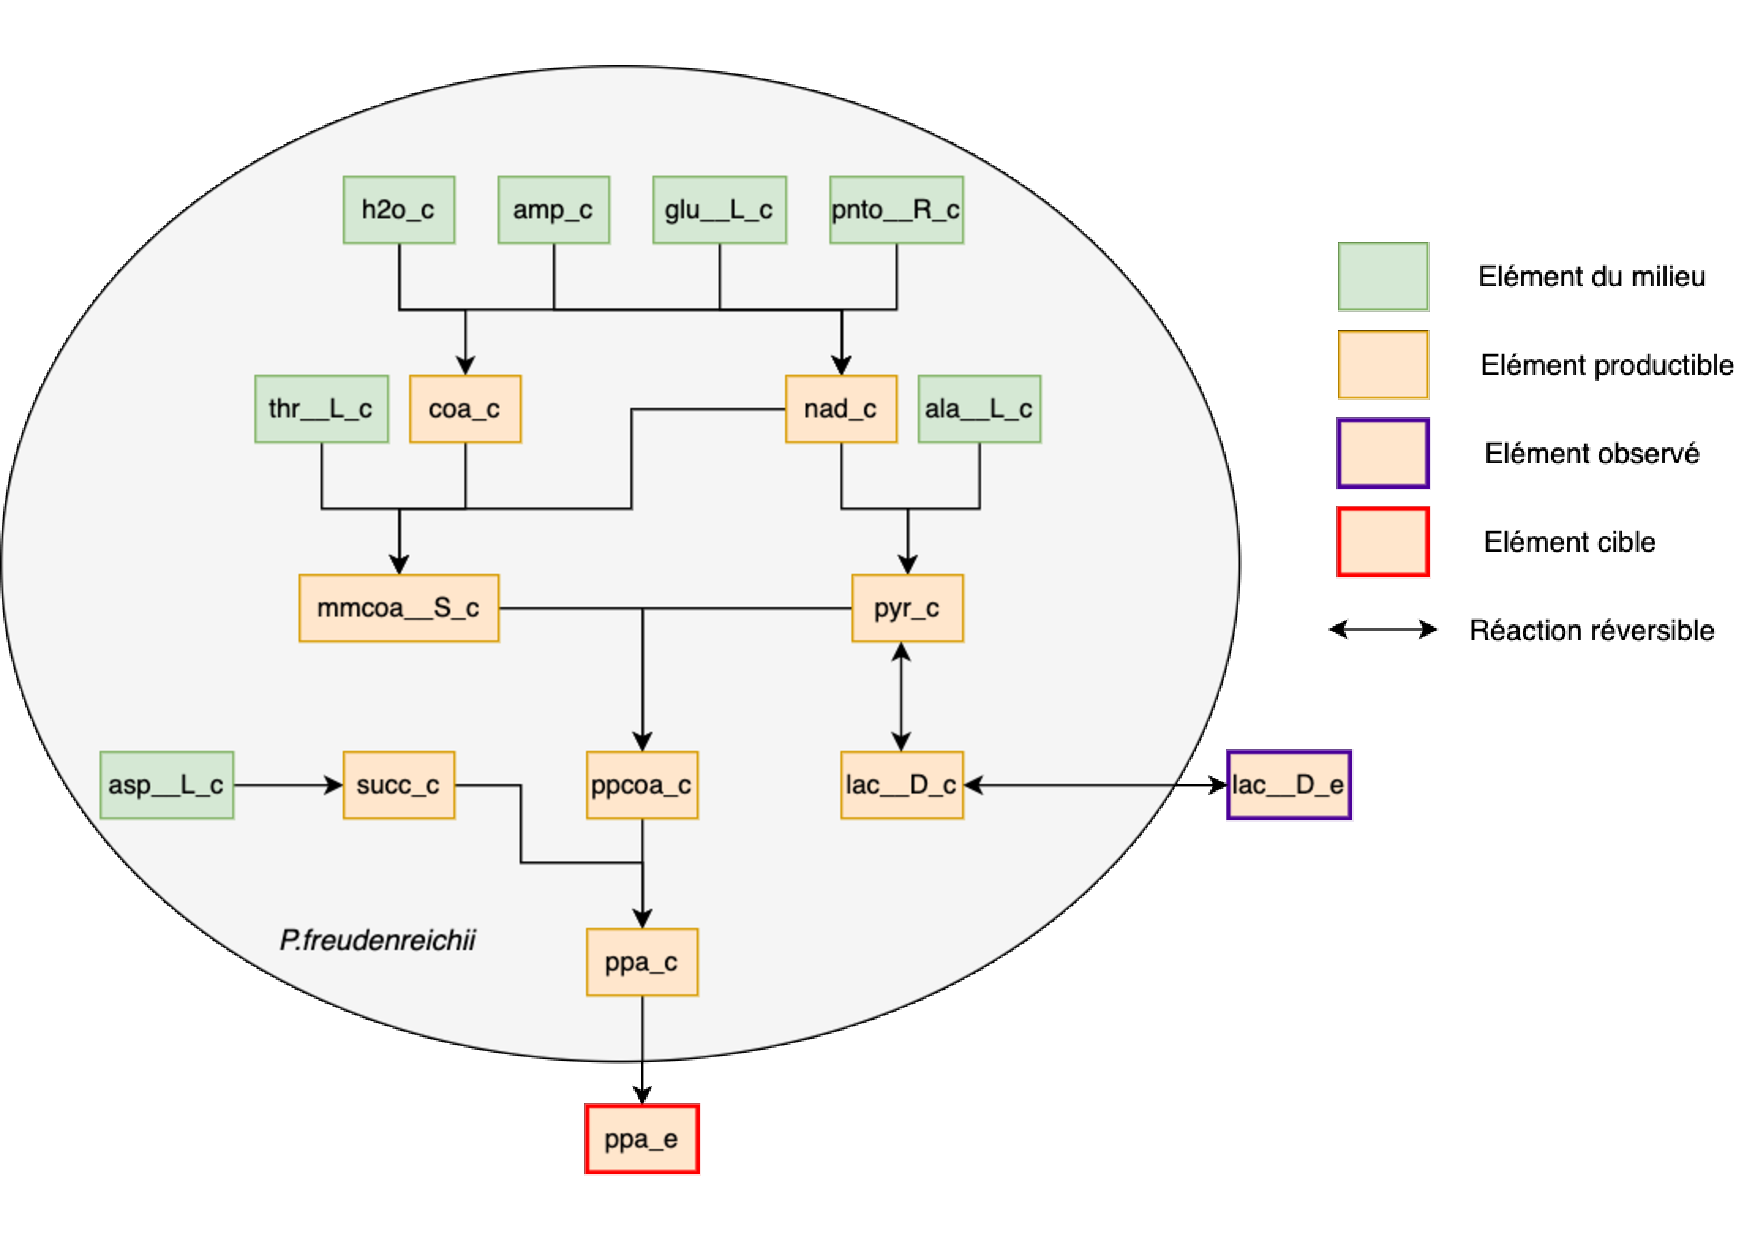
\includegraphics[width=\textwidth]{img/enrichissement/res_simplifie_v2.pdf}
            \caption{Schéma permettant de visualiser le résultat simplifié du modèle d'explication sur les données réelles}
        \label{fig:explication_r}
\end{figure}

Contrairement au cas de planification, il a fallu 23 étapes pour résoudre expliquer la production de propionate à partir du lactate. Malgré l'ajout d'une connaissance \textit{a priori} (consommation du lactate par \freud) le modèle ne permet toujours pas d'identifier les interactions entre les bactéries lactiques et la bactérie propionique. Cependant, nous pouvons reconnaître un cycle important pour la production du propionate: cycle de Wood-Werkman.


\section{Discussion et conclusion}
Nous avons montré une application à la biologie des systèmes d'un concept d'IA: le raisonnement sur les actions et le changement. Nous avons également vu l'efficacité de la temporalité sur les exemples didactiques: des hypothèses sur des interactions bactériennes , explications métaboliques d'observations et rapidité d'exécution. Tout comme dans le chapitre \ref{ccmc}, aucune fonction objective n'est nécessaire. Malgré cela, cette approche permet une description réactionnelle d'une communauté bactérienne.\\

Lors du passage à l'échelle d'un jeu de données réel, nous observons les limites d'une modélisation basée sur la topologie du réseau: production du propionate permise sans échanges métaboliques. Cependant, en sélectionnant les bonnes connaissances \textit{a priori} à inférer dans le modèle, cette modélisation topologique réactionnelle permettrait d'analyser et générer des explications rapidement sur des observations relevées lors des expériences.


\end{document}
% \newpage
% 
%\subfile{chapitres/Discussion.tex}
%%
\documentclass[../main.tex]{subfiles}

\begin{document}
\chapter{Conclusion et perspectives \maxime{NE PAS LIRE}}
%\addcontentsline{toc}{chapter}{Conclusion}
\label{perspective}
%\doublespacing %% For correction

\section*{Discussion}
\addcontentsline{toc}{section}{Discussion}

\textbf{Discussion partie informatique}\\
%explicabilité, import pour les biologistes, nous, informaticiens, sommes là pour ça.
Dans le monde de la biologie, l'identification des mécanismes sous-jacents expliquant une observation est un défi majeur. D'après \citep{lipton2017mythos}, les modèles dit "boîtes-noires" permettent difficilement une interprétation du résultat du modèle, et ainsi ne correspondent pas à la demande des biologistes. A l'opposé, nous retrouvons des modèles "boites blanches" qui, en plus d'identifier des mécanismes responsables de l'observable et d'obtenir une bonne prédiction, permettent d'émettre des hypothèses testables en laboratoire. De ce fait, nous avons développé deux modèles informatiques répondant aux doubles enjeux des biologistes : bonnes capacités prédictives et pouvoir d'explicabilité. En reprenant la terminologie de \citep{lipton2017mythos}, nos modèles assurent donc la \textit{causalité}, \textit{i.e.} l'explicabilité. Parmi les autres critères de \citep{lipton2017mythos}, nos modèles répondent également à la \textit{transparence}, c'est-à-dire, qu'ils peuvent être auditables par les biologistes. Ce critère traite la question de comment le modèle fonctionne, au niveau de l'algorithme, des paramètres  et du modèle entier. \label{contraintes-model}\\


%L'explicabilité permet de générer des hypothèses testables
Le modèle numérique présenté dans le chapitre \ref{tango} modélise un écosystème microbien étudié expérimentalement pour l'élaboration d'un fromage industriel. Pour rappel, notre stratégie itérative consistait à calibrer chaque souche métabolique pour inférer des potentiels d'interaction en communauté. De part cette stratégie, nous avons montré que la prédiction de notre modèle numérique était de bonne qualité. Nos résultats de simulation, à l'échelle de chaque souche métabolique et en communauté, sont numériquement proches des données expérimentales. En raison de cette précision, de la généralité du modèle et de l'utilisation explicite de mécanismes biologiques, nous appelons ce modèle numérique un modèle numérique mécanistique. De plus, la \textit{causalité} du modèle est assurée par l'identification de voies métaboliques activées, de flux de consommation et ou de production ainsi que par la contribution de chaque modèle métabolique. Concernant la souche de \plantarum, nous avons observé pour la première fois en lait l'activation de la voie hétérolactique, représenté par un flux non-nul de la voie de la transketolase. De plus,nous avons observé une utilisation du citrate par \plantarum et une préférence d'utilisation du lactose au regard du lactate par \freud. Notre modèle numérique explique ces résultats par une valeur de xflux de consommation de ces composés. Nous avons également implémenté un partage équilibré des ressources, lorsqu'elles deviennent limitantes, entre les organismes, affinant la prédiction des concentrations des métabolites. Ce mécanisme a permis de mettre en avant les interactions bactériennes révélées dans le chapitre \ref{tango}. Toutes ces explications fournies par le modèle permettent ainsi de générer des hypothèses testables expérimentalement, qualifiant ainsi notre modèle numérique de modèle explicable. Enfin, nous assurons la \textit{transparence} en explicitant les noms des métabolites, des réactions et des voies métaboliques. \\


%Le modèle numérique Tango modélise un écosystème microbien étudié expérimentalement pour l'élaboration du fromage industriel. \\
%La prédiction de ce modèle est de bonne qualité car les résultats sont numériquement proches des données expérimentales \\
%Nous assurons la causalité avec l'activation de voies métaboliques, flux entrant, sortant, contribution chaque souche. [Puis, pour chaque item les détailler.]

%Dans le cadre du jumeau numérique, nous avons implémenté un partage équilibré des ressources entre les membres de la communauté lorsque cette dernière devient limitante (quel critère de succès ? (prediction,causalité,transparence).
%Comme vu dans le chapitre correspondant, cette limitation à pour but d'éviter des valeurs négatives et a permis de déduire des phénomènes d'interactions au sein du consortium bactérien. Au niveau de la communauté, notre modèle explique les concentrations des métabolites suivis en métabolomique en montrant la contribution relative de chaque espèce dans la production ou la consommation de ces composés.


% Créer des modèles explicables pour les biologistes ne permet pas seulement d'expliquer le lien entre les données d'entrée et la sortie, mais également, de générer des hypothèses testables en laboratoire)\maxime{pas utile, introduire par paragraphe ce qu'était chaque modèle en une phrase.}.
%En effet, au sein du modèle numérique de la fermentation du fromage, de nouveaux flux entrants, sortants et nouvelles activations de voies métaboliques peuvent expliquer les observations expérimentales et ainsi être vérifier en laboratoire. A l'échelle de la souche de \plantarum, nous avons mis en avant une activation de la voie hétérolactique en lait, représenté par des flux non nul au sein de la voie métabolique de la transketolase. Ou encore, chez la souche de \freud, une préférence pour consommer le lactose à la place du lactate représenté par une valeur de flux de consommation pour le lactose plus importante. Au niveau de la communauté, notre modèle numérique permet de prédire la contribution de chaque souche en pour la consommation ou la production des composés. Ainsi, l'impact et le rôle d'une souche sur cet écosystème du fromage peut-être testé \textit{in silico} et vérifié expérimentalement. \maxime{rajouter le côté précision numérique (bonne prédiction) et transparence. Elles sont assurées par blabla. La causalité par ce modèle est assurée par ........}

%Chacune de ces items est une hypothèse potentiellement testable. \\
%Comment nous assurons la transparence ? Pour assurer la transparence, on dit les noms de métabolites etc etc.

%Les jumeaux numérique boites blanches diffèrent des boites noirs par l'utilisation explicite des mécanisme bio ainsi que modèle logique
% Nos deux approches, numérique boîte-blanche ou par raisonnement, diffèrent des modèles boîtes noires en répondant au critère de \textit{causalité}, inférant explicitement des mécanismes biologiques, en les formalisant sous forme de contraintes numérique ou de logique pour révéler de nouveaux phénomènes.
% Dans le cadre du jumeau numérique, nous avons implémenté un partage équilibré des ressources entre les membres de la communauté lorsque cette dernière devient limitante. Comme vu dans le chapitre correspondant, cette limitation à pour but d'éviter des valeurs négatives et a permis de déduire des phénomènes d'interactions au sein du consortium bactérien. Concernant l'approche par raisonnement, nous avons formalisé sous forme logique la définition biologique d'un substrat limitant, d'un composé échangeable dans une communauté et révélé un potentiel de coopération et de compétition en se basant sur ces définitions.\\


Le modèle discret du chapitre \ref{ccmc} modélise l'interaction métabolique entre organismes au sein d'un écosystème microbien et prédit le potentiel de compétition et de coopération entre ces organismes. Avec l'approche par raisonnement, nous avons formalisé des définitions biologiques sous forme de règles et contraintes logiques: à partir d'un ensemble nutritif nous calculons le potentiel métabolique pour chaque souche et en communauté; \textit{scope}; les échanges métaboliques; \textit{exchanged}; les substrats en compétition; \textit{polyopsonistic}. Cette formalisation explicite nous permet de calculer des potentiels d'interaction, compétition et coopération, et garantit une bonne confiance dans les prédictions de notre modèle.
D'une part, nos prédiction permettent d'obtenir des résultats similaires ceux fournis les outils numériques existants qui font référence, SMETANA et MICOM, pour les mêmes données.
D'autre part, notre logiciel réussit une batterie de tests induits par un benchmark très complet, que nous avons conçu pour valider les prédictions et scores spécifiques d'un écosystème, évaluer le passage à l'échelle et vérifier le criblage haut débit des communautés.

Tout comme le modèle numérique mécanistique, ce modèle discret assure également la \textit{causalité}: le potentiel de coopération est expliqué par le nombre de métabolites échangés ainsi que par les espèces intervenant dans l'échange; tandis que le potentiel de compétition est expliqué par le nombre de consommateurs associés à un substrat limitant. Ainsi, le proxy de la coopération, représenté par la notion de métabolites échangeables, est expliqué en termes biologiques ainsi: parmi deux organismes A et B, un métabolite est échangeable si, il est productible par l'organisme A et consommable par l'organisme B uniquement lors d'un échange.
De même, la compétition est expliquée en termes biologiques: un substrat nutritionnel est en compétition si ce dernier est limitant et co-consommé. Toutes ces explications issues de notre modèle permettent de générer des hypothèses testables en laboratoire.
La production d'un métabolite échangé entre organismes coopérants A et B peut être détecté en métabolomique par LCMS ou par phénotypage biochimique ciblé, et associé avec la présence ou l'absence de l'espèce A.
La consommation d'un métabolite par deux organismes en compétition peut être testé de façon similaire.

Enfin, notre modèle assure également la \textit{transparence} car chaque règle logique du modèle est lisible, vérifiable et critiquable par les biologistes. En reprenant la notion biologique de coopération plus haut, un métabolite est dit échangé s'il est dans le \textit{scope} d'un producteur, qu'il soit reactant d'un consommateur et qu'il ne soit pas dans le \textit{scope} du consommateur.
%Le modèle discret modélise l'interaction métabolique entre organismes microbiens dans un écosystème microbien et prédit le potentiel de compétition et la coopération entre ces organismes. \\
%Les prédictions de ce modèle sont bonnes pour deux raisons: la première est que nos résultats sont au moins aussi bons que des outils numériquement plus coûteux. d'autre part, à l'aide d'un benchmark répondant à nos attentes. \\

%Comment nous assurons la causalité ? le nombre de métabolites échangés, le nom des espèces intervenant, le nombre d'espèces intervenant.  donner un exemple pour la compétition: ça veut dire qu'il existe, pour un métabolite limitant, un nombre de consommateurs supérieur à 1. donner l'exemple pour la coopération également. \\
%Comment nous assurons la transparence ? Tout cela est dû au fait que chaque inférence suit une règle biologique, et lisible et critiquable par les biologistes.\\

%D'autre part, notre modèle par méthode de raisonnement, en plus de pouvoir passer à l'échelle, est intrinsèquement lié à la famille de modèles interprétables. En effet, grâce à la méthode de résolution de Clingo, l'ensemble de réponse qui en résulte satisfait les contraintes et règles logiques écrites et ainsi, éviter des possibles biais dans la résolution. Ce pouvoir de modélisation explicable par nature permet de soulever des hypothèses testables sans processus d'inférence numérique coûteuse. En effet, le nombre de métabolites échangés ainsi les espèces productrices et consommatrices intervenant dans ces échanges, la plus value d'ajouter ou retirer une espèce, génèrent des hypothèses testables rapidement.\\




%À partir des besoins des bio, je peux les aiguiller sur la nature de la modélisation. Développer
% Ces deux approches ont montré qu'ils sont plus ou moins appropriés aux besoins des biologistes. \maxime{ne pas hésiter à illustrer les questions que l'on se pose -> quelles voies activées : numérique etc etc}. \maxime{C'est le moment de mettre mon tableau. }
Les modèles explicables développés dans cette thèse ont été élaborés pour répondre avec précision à des enjeux biologiques précis. Dans les deux cas, identifier la bonne méthode correspondante à ses enjeux n'a pas été trivial mais la conclusion d'une analyse menée en concertation avec les collègues biologistes.
Le critère que les modèles doivent être prédictifs et explicables ne permet pas en soi de choisir entre un modèle numérique et discret.

% Enjeux que l'approche discrète répond: passage à l'échelle, hypothèse de compétition/coopération, explication mécanistique, ordonnancement d'évènement (temporalité), sélection de consortium bactérien, comparaison de communauté, scope

L'approche discrète développée répond à de multiples enjeux que sont: la résolution de problèmes combinatoires permettant de passer à l'échelle de communautés naturelles, d'émettre des hypothèses sur de potentielles interactions bactériennes, d'apporter une explication structurelle des phénomènes observés, d'obtenir des \textit{scope} de métabolites productibles et consommées par un plusieurs organismes et d'obtenir une précision des résultats dû à l'inférence des règles biologiques. Chacun des modèles mécanistiques que nous avons développés permet de répondre à ces enjeux plus ou moins efficacement. Le modèle numérique a démontré sa polyvalence pour répondre à ses enjeux et est particulièrement adapté pour donner une dimension numérique de l'explicabilité, de scope métaboliques et des hypothèses testables. Lee modèle par raisonnement est quant à lui pertinent pour sa capacité à déterminer des potentiels d'interaction pour des grandes communautés en résolvant des problèmes combinatoires et de passer ainsi à l'échelle. De plus, ce modèle procure une explication détaillée et rapide du fonctionne de la commauté: par exemple, l'ensemble des métabolites échangés ainsi que les ensembles de producteurs et de consommateurs intervenant pour l'échange de ce métabolite. En somme, chaque enjeu peut être résolu par un modèle, et donc, un unique modèle hybride n'est pas forcément nécessaire.


% En revanche, le degré de précision le permet. Par exemple, les deux modèles permettent de montrer des voies métaboliques activables, mais seul le modèle numérique permet d'identifier celles qui sont réellement activées ou non à un temps donné. Le modèle discret permet de définir des ensembles de métabolites productibles tandis que le modèle numérique précise en quelle quantité ils sont produits. Enfin, le modèle numérique est adaptable sur des écosystèmes contrôlés alors que le modèle discret est généralisable sur des écosystèmes naturelles composés de plusieurs centaines de bactéries. Ainsi, le modèle numérique avait pour enjeu de créer un modèle de fermentation du fromage en reproduisant les concentrations observées expérimentalement. Le modèle discret était focalisé sur la comparaison au débit de potentiels de coopération et de compétition d'écosystèmes microbiens. Ce travail a démontré qu'à élaborer un modèle hybride pour la modélisation l'écosystème microbien n'est pas nécessaire, mais que la difficulté était de choisir le modèle le plus efficace pour répondre à l'enjeu biologique.
%Ces modèles, logiques et numériques, ont montré leur capacité à expliquer les mécanismes cachés à partir d'un enjeu biologique. En revanche, choisir la bonne méthode pour répondre à ses enjeux n'est pas trivial. Nous avons pour cela dû formaliser des enjeux à partir de discussions entre experts. Nous pouvons classer ces enjeux en deux familles: la précision des résultats et la flexibilité du modèle. A partir de ces deux classes nous pouvons recommander l'utilisation d'un modèle numérique ou d'un modèle logique en prenant en compte les possibles limites de ces modèles par rapport aux enjeux biologiques. Ainsi, pour une reproduction fidèle des données expérimentales, un modèle numérique comme celui du chapitre \ref{tango} conviendrait mieux. En revanche, dans un but de construction de consortium bactérien, de comparaison de communauté bactérienne ou encore d'ordonnancer des processus de manière haut débit, un modèle discret est plus adapté.

Notre étude permet cependant d'évaluer l'opportunité que représente la construction des modèles hybrides pour des écosystèmes microbiens complexes.
Quelles auraient été les propriétés d'un modèle hybride, combinant les avantages de la précision numérique d'un jumeau numérique avec celles du passage à l'échelle de communautés naturelles d'un modèle discret.
Dans un soucis de satisfaire les contraintes explicitées dans le paragraphe \ref{contraintes-model}, ce nouveau modèle hybride doit toujours être explicable, en donnant de bonnes prédictions numériquement proches des valeurs expérimentales et qu'il puisse identifier des potentiels d'interaction à grande échelle dans le but de générer des hypothèses testables sur les voies métaboliques activées, les espèces impliquées dans un échange métabolique ou encore celles en réelle compétition.




% Dans un souci de satisfaire les biologistes, ce modèle hybride doit toujours être explicable, c'est- à dire, promouvoir de bonnes prédictions, et générer des hypothèses testables.
Deux pistes peuvent être explorées : améliorer le passage à l'échelle du modèle numérique ou enrichir le modèle discret. Nous avons opté pour le second choix en proposant un premier enrichissement temporel. En utilisant la logique temporel \citep{Cabalar2019}, il est possible, à l'aide de règles logiques temporelles, d'identifier quand un métabolite est productible. Cet ajout temporel permettrait d'affiner la prédiction du potentiel de compétition: deux espèces sont en compétition si pour un même substrat limitant, au moins deux espèces le consomment \textsl{au même moment}. Nous avons par la suite permis la sélection de communauté pour la construction d'un design expérimental. Cet ajout permet d'améliorer l'explicabilité du modèle puisque chacun des modèles proposés par le modèle discret est expliqué par les critères de sélection en amont.

Le modèle numérique représente le but final à atteindre de part sa précision numérique. Pour améliorer son passage à l'échelle, les paramètres inférés pour chaque souche métabolique peuvent être déduits à partir d'un méta-modèle pré-entraîné \textbf{(ref)}. Dans un second temps, le flux de consommation et de production peut être calculés à partir de la concentration des métabolites d'intérêt à chaque point de temps. Enfin, nous pouvons discrétiser le temps et calculer un FBA dans un intervalle de temps plus important, réduisant ainsi le temps de calcul mais augmentant l'approximation entre deux pas de temps.



% Cette étude à montrer que nous n'avons pas eu besoin de faire un modèle hybride. mais qu'elle aurait été les propriétés du grand modèle hybride en combinant les avantages de ccmc et tango? [Il faut reprendre les étapes : en quoi il ferait de bonnes prédictions, etc ON VEUT TOUJOURS QU'IL SOIT EXPLICABLE : \emph{causalité} et \emph{transparence}.]
% Deux pistes: soit du numérique vers le passage à l'échelle soit du discret vers un enrichissement.
% Pourquoi enrichir le discret est mieux ?
% Type d'enrichissement: un métabolite est compétitif si deux espèces consomment en même temps ce métabolite sans la nécessité de parler de concentrations ; un métabolite est témoin de la coopération si ...

% Travaux futurs: à quoi ressemble le tango en mode hybride ? Est ce que ca serait toujours générateur testable ?
%\maxime{uniformiser les mots : numérique ? jumeau? discret}
\maxime{expliciter pourquoi c'est dur LCMS, car c'est la résultant production-consommation}
%\maxime{page 5 reformuler scope/iscope}
\maxime{'prise en compte de la temporelle' dernier paragraphe}

\textbf{Discussion partie biologique}\\
%Comment la modélisation par topologique et en flux peut aider le biologiste à identifier les interactions bactériennes favorables et défavorables au fonctionnement de l’écosystème ?

La fermentation bactérienne est au c\oe{}ur de la fabrication fromagère et elle se caractérise par une acidification du milieu, une production de composés d'arômes et enfin par une croissance bactérienne. Les échanges de métabolites entre espèces favorisent le fonctionnement de l'écosystème.

%Comme nous avons pu le voir dans cette thèse, la modélisation discrète et en flux ont permis de générer des hypothèses testables sur les interactions bactériennes favorables et défavorables au fonctionnement de l'écosystème. Dans le chapitre \ref{tango}, la fermentation bactérienne était le c\oe{}ur du sujet se caractérisant par une acidification du milieu, une production de composés d'arômes et enfin par une croissance bactérienne pour la production de fromage. Dans le cas de la modélisation discrète du chapitre \ref{ccmc}, nous nous sommes plus intéressé aux potentiels métaboliques, i.e. de production, de consommation, de coopération, de compétition etc. \\

L'approche discrète du chapitre \ref{ccmc} identifie des hypothèses biologiques en comparant des ensembles, de métabolites produits et consommés, par entité biologique au sein d'un écosystème. Parmi ces ensembles, nous avons calculé les ensembles de métabolites: (i) échangeables entre différentes souches, (ii) déjà présents dans le milieu extra-cellulaire, (iii) nouvellement disponibles libérés au cours d'une fermentation bactérienne par exemple, (iv) pouvant être limitant. L'analyse comparée de ces ensembles a permis de prédire les espèces en compétition, les échanges et les souches impliquées dans les échanges. Ces échanges peuvent impacter la croissance des bactéries, la production de composés d'intérêts et le pH. En plus de l'identification d'interactions en comparant des ensembles, nous avons calculé des potentiels de coopération et de compétition, ce qui ajoute une dimension pseudo-quantitative à l'interaction et permet de comparer des communautés de divers écosystèmes entre eux.

La dimension quantitative d'une interaction bactérienne est apportée par le modèle numérique mécanistique du chapitre \ref{tango}. Cette dimension est caractérisée par la prédiction de la concentration des métabolites, et la quantité de biomasse produite, correspondant au taux de croissance de l'espèce. Les interactions sont identifiées en analysant les flux de métabolites (i) entrant dans la cellule bactérienne et (ii) sortant vers le milieu extracellulaire. Par exemple, à l'échelle de chaque cellule, tous les modèles métaboliques ont un flux de consommation du lactose non nul, suggérant une compétition pour ce dernier. Ou encore, le lactate est produit par les bactéries lactiques et consommé par \freud symbolisé respectivement par un flux de lactate sortant et entrant. Ces mécanismes révèlent une coopération entre les bactéries lactiques, \plantarum et \lactis, et la bactérie propionique \freud. Cette analyse est faite grâce aux méthodes d'analyse par  contrainte des flux (FBA, FVA) \citep{Orth2010, Mahadevan2003}sous l'hypothèse de  maximisation de la biomasse. Il est possible de faire varier cette fonction objective, par exemple maximisation de la synthèse d'ATP ou de lactate, la distribution des flux changerait et donc, de nouvelles hypothèses d'interactions verraient le jour.

Ces interactions ont des impacts cinétiques sur la concentration des composés d'arômes et sur la densité bactérienne. Au cours du temps, la concentration et la densité bactérienne varient, et une croissance nulle ou ralentie d'une souche peut-être expliquée par une compétition pour un substrat ou par un précurseur limitant, au sens biologique. La production d'un composé d'arôme peut également être ralentie ou annulée, suggérant également une compétition. Ces hypothèses ont été mises en avant par une analyse dynamique de l'équilibre des flux (DFBA) \citep{Mahadevan2002} et a permis de proposer des valeurs de contribution relative de chaque espèce à la consommation et la production de composés d'intérêts. Nous avons ainsi suggéré une indication des producteurs et des consommateurs pour chaque composé pouvant être testés en laboratoire. La validation biologique pourrait être réalisée par un knockout des gènes correspondants. En plus de ces impacts, nous avons pu déduire quelles sont les espèces participant le plus à l'acidification du milieu, au regard de notre modèle de pH. \\



%Quels aller-retours peut-on envisager entre modélisation et expérimentation biologique pour affiner cette compréhension ? en gros … Si on devait refaire le projet Tango toi et moi en partant de zéro, comment arriver à un résultat d’identification d’interaction au moindre effort ? peut-on introduire plus tôt la modélisation ? Est ce que la metaT était indispensable ? …
Les deux approches, discrètes et numériques que nous avons développées dans cette thèse, ont permis de générer des hypothèses testables, affinant la compréhension des interactions qui favoriserait la croissance bactérienne et/ou la production de métabolites. A partir de ces hypothèses, nous discuterons des expérimentations biologiques permettant de valider ou d'invalider les hypothèses afin d'améliorer les modèles explicatifs. Nous traiterons uniquement le cas où des génomes annotés et les souches correspondantes sont à notre disposition. \\


Les approches numériques et discrètes que nous avons développées ont permis de détecter des interactions bactériennes. Dans le cas d'un échange de métabolites entre deux souches, nous avons pour les deux approches la bactérie productrice et consommatrice ainsi que le sens de l'échange. Par exemple, le lactate, mis en avant par notre implémentation du dFBA, est produit par les bactéries lactiques et consommés par \freud, la phénylalanine, révélée par SMETANA \citep{Zelezniak2015} et MiCOM \citep{diener2020}, produite par \plantarum et consommée par \freud. Ces deux approches approches permettent également de nous indiquer des souches co-consommatrice de substrats qui peuvent conduire à une compétitionentre souches si c'est substrats devenaient limitants. Par exemple, le lactose, co-consommé par les consortium, ou encore la glycine, produite par \plantarum et co-consommée par \lactis et \freud. Toutes ces interactions révélées \textit{in silico} avec des outils \textit{a priori} ou \textit{sans a priori} peuvent être validées expérimentalement au moyen d'une comparaison entre des co-cultures et des cultures pures. Afin de vérifier l'impact de ces interactions, la comparaison se porterait sur la croissance des bactéries ainsi que sur le dosage de métabolites.

Dans le cas d'une hypothèse de co-consommation d'un substrat, une décroissance bactérienne et/ou une diminution de la concentration de ce métabolite devraient être observées en co-culture. Afin de vérifier les souches impliquées, un marquage isotopique à froid de ce métabolite suivi d'une spectroscopie avec la méthode Raman \citep{Wang2020,CUI2022100187} permettrait d'identifier les consommateurs de ce métabolite. 
% Dans le cas d'une coopération syntrophique, i.e. où nous avons un échange d'une productrice vers un consommateur, il existe des sous-cas pouvant expliquer l'observation en co-culture. Le premier point attendu est une \textit{sous production} de ce métabolite échangé. Il existe, à notre connaissance, 3 hypothèses biologiques pouvant expliquer cette observation, pouvant être: (1) une inhibition de la croissance de la bactérie productrice empêchant la production de ce dernier, un échange métabolique et/ou une répression transcriptionnelle ou traductionnelle de la voie de synthèse de ce métabolite par l'espèce productrice. Le second point se traduirait par une \textit{sur production} de ce métabolite. Il existe également 3 hypothèses biologiques pouvant expliquer cette observation : croissance bactérienne favorisée, activation du processus de production et/ou échange d'intermédiaires métaboliques.  
 Les activations et les inhibitions de productions métaboliques peuvent être mises en avant avec les données méta-transcriptomique ou métaprotéomiques. Pour révéler expérimentalement ces échanges d'intermédiaires métaboliques (1), il faut valider indépendamment la production de ce métabolite par l'espèce productrice en culture pure et la consommation par l'espèce consommatrice avec un marquage isotopique.

%Comme indiqué plus haut, la méthode de jumeau numérique a permis de mettre en évidence des interactions en comparant les flux d'entrée et de sortie des modèles métaboliques avec des méthodes de flux statique. Cette comparaison met en évidence les métabolites échangés, les espèces qui relarguent le métabolite et les espèces qui le consomment. En mettant en place une comparaison des cultures pures de chaque espèce avec les espèces en co-culture, du point de vue des dosages  biochimiques, nous pouvons identifier les acteurs de l'interaction.
%Pour vérifier qu'elles sont les consommateurs, le métabolite échangé peut-être suivi avec un marquage isotopique. Lors d'un dFBA avec communauté, nous avons en plus le dynamisme du métabolisme de communauté au cours du temps. Dans un premier temps, les flux de production et de consommation de chaque espèce pour chaque métabolite ainsi que la concentration de ce dernier. Pour vérifier les interactions mis en évidence par cette donnée, l'usage de données metatranscriptomiques ou de métaprotéomique peut servir à les valider ou à les réfuter, en regardant l'expression des gènes associés au réactions.
%
%En comparant notre approche \textit{a priori} avec des méthodes \textit{sans a priori}, SMETANA et MiCOM, nous avons évalué les potentiels interactions que notre communauté fromagère peut développer. Nous avons pour chacun des outils des ensembles de métabolites échangés ainsi que les orientations des échanges. Comme précédemment, une comparaison pure/co-culture peut-être faite afin d'identifier les productions individuelles et utiliser un marquage isotopique afin d'identifier les consommateurs. Enfin, une validation avec des données métaTranscriptomique et métaprotéomique peut être faite. \\

%Contrairement à notre méthode de jumeau numérique, notre modèle discret a mis en avant les interactions en se basant sur des ensembles: métabolites échangés (1), souches qui participe à ses échanges ainsi que le sens (2) ainsi que des souches qui consomme le même substrat appartenant au milieu de culture et à l'ensemble des métabolites échangés (3).  En utilisant une comparaison de pure culture et de co-culture des croissances bactériennes et d'un dosage métabolique pour chaque espèce en cinétique , les points (2) et (3) peuvent être vérifiés. Dans le cas d'une hypothèse de co-consommation (3), une décroissance bactérienne ou/et une diminution de la concentration de ce métabolite serait observé. Dans l'identification des souches (2),  deux cas peuvent avoir lieu. Dans le premier cas, une \textit{sous-production} de ce métabolite échangé en co-culture est observée. Les hypothèses biologiques sous-jacentes expliquant cette observation sont les suivantes: une inhibition de la croissance bactérienne empêchant la production de ce métabolite, un échange métabolique ainsi que le sens de l'échange et enfin, une inhibition de la production de ce métabolite par l'espèce productrice. Dans le second cas, une \textit{sur-production} de ce métabolite est observé en co-culture. Les hypothèses biologiques expliquant cette observation sont les suivantes: croissance bactérienne favorisée, activation du processus de production et un échange d'un intermédiaire métabolique. Les activations et les inhibitions de productions métaboliques peuvent être mis en avant avec les données méta-transcriptomique ou métaprotéomiques. Pour révéler expérimentalement ces échanges d'intermédiaires métaboliques (1), il faut valider indépendamment la production de ce métabolite par l'espèce productrice et la consommation par l'espèce consommatrice. \\

\textbf{Retour d'expérience de la thèse}\\
Au cours de la collaboration établie avec les biologistes dans cette thèse, nous avons pu mettre en évidence deux façons d'exploiter les modèles développés. Dans un premier temps, seul le \textit{résultat} du modèle est important afin de vérifier expérimentalement les prédictions. Par exemple, au sein du chapitre \ref{tango}, nous avons mis en avant de nouvelles interactions métaboliques potentielles, à la fois avec notre modèle  avec \textit{a priori} et les outils \textit{sans a priori}, pouvant être validées ou réfutées grâce aux moyens que nous avons développés plus haut. Dans un second temps, pour une réexploitation des résultats de la thèse, la propriété de \textit{généricité} des outils et du savoir-faire est importante. Cette généricité permet l'utilisation pour une autre question de recherche ou avec des données d'entrées différentes. Par exemple, les outils développés des chapitres \ref{ccmc} et \ref{enrichissement} ont permis l'utilisation de réseaux métaboliques appartenant à n'importe quels écosystèmes, et permettent de s'intéresser à la compétition, coopération, sélection de communautés selon différents critères biologiques etc. Également, le degré de \textit{diffusion} des logiciels développés est un facteur à prendre en compte pour un travail interdisciplinaire. En effet, le déploiement de nos outils sur une plateforme, telle que Galaxy \citep{10.1093/nar/gkac247} par exemple, permettrait de garantir un accès simplifié pour les biologistes et d'approfondir leur recherche sur la compréhension des interactions bactériennes.


\section*{Bilan des contributions}
\addcontentsline{toc}{section}{Bilan des contributions}

Au sein des travaux de cette thèse nous avons développé plusieurs méthodes d'analyse de communautés microbiennes applicables à des communautés appartenant à un écosystème simplifié, ou bien, à des communautés simulées provenant d'écosystèmes naturels complexes, en proposant dans un premier temps de caractériser la coopération et la compétition au sein d'une communauté et dans un second temps, de proposer un modèle de sélection de communauté pour permettre l'analyse numérique de communautés intéressantes.\\
Notre méthodologie numérique se base sur la connaissance \textit{a priori} du système biologique d'étude ainsi que sur la grande disponibilité des données. Ainsi, notre approche itérative devrait être applicable pour toute communauté où ces contraintes sont respectées. En effet, le raffinement de chaque modèle est un processus universel consistant à ajouter, éteindre ou modifier des réactions. En se basant sur l'analyse de la variance des flux et de la connaissance avec \textit{a priori}, les chemins métaboliques utilisés ont pu être déterminés et la cohérence de ces résultats vis à vis de la littérature a été vérifiées. De plus, l'ajustement des mécanismes biologiques, tels que la consommation du lactose ou du lactate, à travers l'optimisation des paramètres, a été déduit en observant les courbes de simulations dynamiques. Enfin, nous avons montré qu'il était possible, à partir d'un mécanisme équitable de partage des ressources et d'un "tunning" à l'échelle de chaque bactérie, de mettre en avant des interactions bactériennes en communauté et d'obtenir des prédictions numériques satisfaisantes. Ces résultats ont fait l'objet d'un papier soumis dans metabolic engineering.\\

Nous avons par la suite cherché à définir les limites de l'analyse des interactions microbiennes dans le cas le plus pauvre, c'est-à-dire, avec uniquement des données génomiques. En basant notre méthodologie développée sur le principe de raisonnement et construit comme une extension du logiciel MISCOTO \citep{Frioux2018}, les propriétés  d'explicabilité des modèles et le passage à l'échelle de communautés de grande taille ont été conservés. Grâce à cette approche d'abstraction booléenne, nous avons caractérisés des potentiels de coopération et de compétition permettant une comparaison de communautés entières et non deux à-deux. Même si la méthode n'a pas la précision des approches numériques, elle compense par sa capacité de criblage au débit, permettant d'effectuer un premier filtre de caractérisation de l'écosystème microbien. Lors de la comparaison avec des méthodes quantitatives, nous avons démontré que la tendance de nos scores, issu d'un raisonnement booléen, était corrélée avec des méthodes basées sur des méthodes par contrainte. De part le faible temps d'exécution de notre approche, ces résultats confortent l'utilisation d'une méthode moins précise mais peu coûteuse pour permettre d'identifier manuellement des ensembles considérés pertinents du point de vue de la compétition, de la coopération, des substrats limitants ou bien des métabolites échangeables. Enfin, nous démontrons l'indépendance de notre approche vis-à -vis de la méthode de reconstruction des réseaux métaboliques ainsi que de l'écosystème d'origine des génomes. \\

Nous avons par la suite cherché à enrichir ces modèles logiques du point de vue de l'identification de communautés pertinentes en ajoutant des contraintes fournies par l'utilisateur ou l'utilisatrice. En effet, dans un monde idéal, un modèle hybride où le formalisme logique et numérique communiquent, permettrait à la fois une sélection de communautés pertinentes et une analyse numérique de ces dernières. La méthode de \citep{Frioux2018} est une première étape dans la construction d'un tel modèle qui sélectionne uniquement des communautés minimales, en minimisant le nombre d'échanges métaboliques au sein de la communauté. En s'inspirant de cette méthode, nous avons contruit un prototype qui, à partir d'un ensemble de réseaux métaboliques, l'utilisateur ou l'utilisatrice peut sélectionner une communauté en filtrant sa taille, sa composition taxonomique, le nombre de métabolites cibles devant être produits. Par ailleurs, l'ordre et le choix d'optimisation est également libre à l'utilisateur ou l'utilisatrice. Grâce à ce travail, la taille de l'ensemble de communautés trouvés, respectant les règles et les contraintes logiques définies en amont, est réduite et l'utilisation d'un modèle numérique précis et performant sur des communautés de petites tailles peut être ainsi utilisé. Ce travail, vers un modèle hybride, est l'objet d'un papier scientifique en cours de rédaction.

\newpage
\section*{Perspectives}
\addcontentsline{toc}{section}{Perspectives}

Avec ces trois chapitres, nous avons contribué à l'avancement des analyses des communautés microbiennes sur le plan numérique et discret. Cependant plusieurs points d'amélioration subsistent. A court terme, valoriser davantage l'intégration des données métatransciptomiques serait intéressant. En effet, dans le chapitre \ref{tango}, nous avons utilisé ces données hétérogènes pour valider des interactions mises en évidence par SMETANA en regardant l'expression des gènes associés à la production et à la consommation des métabolites présumés échangés. Il pourrait être intéressant de contraindre les réseaux métaboliques avec les données méta-transcriptomiques avec différentes méthodes \citep{Jenior2020,Agren2012,Becker2008} et de les comparer avec nos données simulées au niveau des voies métaboliques exprimées ainsi que par rapport aux données de métabolomiques. De plus, nous pourrions nous demander si seul les régulations des expressions géniques suffisent pour obtenir un modèle numérique précis, ce qui aurait pour conséquence de réduire le temps passé au raffinement et à la  calibration de modèles métaboliques. Ces données pourraient également servir de contrainte \textit{a priori} pour les modèles discrets du chapitre \ref{ccmc} et \ref{enrichissement}. En effet, inférer des règles logiques sur l'expression de voies métaboliques connues peut changer les potentiels d'interactions de communautés microbiennes. \\

À moyen terme, la construction d'un modèle hybride des écosystèmes microbiens pourrait être faite. Même si nous avons conclu qu'un modèle hybride n'est pas nécessaire, ce type d'approche pourrait apporter une plus-value. En effet, les métabolites suivis en dynamique dans le modèle numérique du chapitre \ref{tango} proviennent d'une question biologique. Coupler ce modèle numérique à une approche de criblage, comme le modèle logique du chapitre \ref{ccmc}, permettrait de fournir des métabolites d'interêts en entrée. Une difficulté mise en évidence, est le grand nombre de composés échangés détecté par une telle approche. Dans le but de filtrer ces solutions, un premier apport du modèle numérique serait de vérifier la faisabilité de production des composés identifiés par le modèle logique. Cette faisabilité pourrait-être transmise aux modèles logiques comme une donnée d'entrée sous forme de règles et ou contraintes. Nous aurions à terme, un modèle hybride couplé où le formalisme numérique et le formalisme discret communiquent permettant l'analyse de communautés microbiennes.\\

Enfin à plus long terme, la construction d'un modèle de jumeau numérique du processus de la fermentation bactérienne. Selon la définition de L'INRAE, un jumeau numérique est "défini comme une représentation numérique de l'object ou du système d'intérêt  (physique ou biologique ; e.g. cellule, tissu, plante, animal), incluant des variables décrivant son état et son évolution de façon dynamique" \footnote{\url{https://digitbio.hub.inrae.fr/thematiques/vers-le-jumeau-numerique\#Jumeaux}}. Nous avons des données d'entrée dynamique sur le processus de fermentation (métatranscriptomique, métabolomique et cinétique), un algorithme de modélisation et de simulation. Une caractérisation manquante est la boucle de rétroaction du modèle sur l'état du processus modélisé: \textit{i.e.} une prise de décision.



%Les analyses du chapitre \ref{tango} ont révélé des interactions biotiques permettant d'expliquer les observations biologiques. Les données méta-transcriptomiques ont été seulement utilisées pour valider ou réfuter les échanges métaboliques \textit{ad hoc}, et n'ont pas été utilisées pour contraindre les GEMs.  Le consortium bactérien analysé au sein de ce chapitre fait partie d'un projet industriel où l'impacte des facteurs abiotiques, comme la température, ont analysé. Une amélioration possible du modèle numérique serait de prendre en compte ces facteurs abiotiques dans le modèle dynamique. Toujours en se concentrant sur les réseaux métaboliques, \citep{Pettersen2023} ont effectué de l'inférence de paramètre de température sur les modèles métaboliques à l'échelle du génome. \\
%
%Dans le chapitre \ref{ccmc} et surtout le chapitre \ref{enrichissement}, nous nous sommes focalisés sur l'analyse à grande échelle de communautés bactériennes en apportant une notion pseudo quantitative, avec les scores de coopération et compétition, et en filtrant des communautés candidates. Dans l'optique d'apporter plus de précision dans chacun de ces modèles, nous pouvons utiliser la méthode d'analyse par équilibre des flux présenté dans le chapitre \ref{ch:edla} pour contraintes les ensembles de solutions. Il existe clingoLP \citep{Janhunen2017}, une extension du solveur clingo pour la résolution de contraintes linéaires. En effet, dans \citep{Thuillier2022}, ils utilisent un solver intégrant des contraintes linéaires dans de l'ASP pour modéliser l'hypothèse que le système est à l'équilibre. Ainsi, les proxy de la coopération et de la compétition, que sont respectivement les métabolites échangeables et les substrats limitants, identifiés grâce aux contraintes logiques seront restreint avec les contraintes linéaires. Un deuxième point d'amélioration des méthodes logiques est la prise en compte de l'abondance relative des espèces, connu pour impacter le rôle dans un écosystème \maxime{ref dans micom je crois}. Avec l'utilisation du solveur linéaire clingoLP, où les nombres flottants peuvent être pris en compte, avec l'analyse en flux dans le modèle ASP, la prise en compte d'une abondance relative pourrait être faite. \\
%Du point de vue du calcul du score de coopération et de compétition implémenté dans le chapitre \ref{ccmc}, ces derniers utilisent le vocabulaire généré par le solveur logique pour calculer les indices à l'aide du langage de programmation Python. Afin de faciliter l'intégration et son déploiement sur différentes architectures logicielles, trouver un moyen de le calculer directement en ASP serait une plus value. \\
%Enfin, dans le chapitre \ref{enrichissement}, une proposition d'intégration temporelle au sein du formalisme logique a été faite. Nous sommes partis du postulat que le formalisme Telingo, s'inspirant du formalisme logique utilisé dans le chapitre \ref{ccmc}, puisse passer à l'échelle. On remarque tout d'abord que sans aucunes contraintes \textit{a priori}, le nombre de modèles possible explose. Ainsi, une première façon de procéder serait d'ajouter des règles logiques à partir de cas concrets d'observations afin d'éviter d'observer des faux-positifs, et ainsi diminuer les sorties de modèle. Une autre amélioration possible concerne l'intégration du temps. En effet, le temps est représenté comme une séquence d'action ordonnée discrète et non comme une dimension dynamique continue. Un premier travail consisterait à implémenter cette dynamique à l'échelle d'un organisme pour suivre la production ou la consommation de métabolites.


%\section{Approches hybrides découplées et couplées}
%L'approche de modélisation hybride développée dans cette thèse à été développée sous de multiples angles. La première est la création d'une approche hybride découplé, avec les projets TANGO et CoCoMiCo. Chacun des deux permet de caractériser une communauté bactérienne en mettant en avant les interactions entre bactéries. TANGO et CoCoMiCo apportent une information supplémentaire et complémentaire sur la communauté bactérienne. Ces deux approches sont complémentaires du fait du raisonnement utilisé dans le modèle logique, le criblage permet de mettre en avant l'ensemble de interactions métaboliques possibles en fonction de l'environnement nutritionnel et peut ainsi servir de support pour inférer les éléments à suivre dynamiquement dans le modèle dynamique (modèle hybride couplé). La modèle dynamique quand à lui, permet à partir d'une base de fait établie, issu de la connaissance biologique, de la littérature ou bien d'un logiciel de criblage, de décrire avec précision des mécanismes de régulation et entre autre, des interactions bactériennes.\\

%En plus de la fiabilité des éléments criblés à vérifier, réduire leur nombre ainsi que obtenir un population microbienne minimale est nécessaire afin d'utiliser des systèmes dynamiques tels que celui de TANGO. En effet, plus le nombre de paramètres à suivre augmente, plus le temps de calcul croit. Plusieurs questions surviennent alors quant aux critères de sélection permettant de mettre en place un filtre efficace. Dans \citep{Frioux2018}, les auteurs proposent de sélectionner une communauté bactérienne basée en minimisant la taille de la communauté. En fonctionnant ainsi, minimiser la taille ne permet pas de garantir que la communauté finale est la meilleure pour répondre à un objectif. En effet, il permet de résoudre la combinatoire du nombre de communauté bactérienne que le programme résout.

%\ifdefined\FromMain %
%\else %
 \end{document} %




%\newpage
%
%
%\chapter*{Reference}
%\addcontentsline{toc}{chapter}{Reference}
%\bibliographystyle{apa}
%\setcitestyle{numbers}
%\bibliography{reference}
%
%
%\appendix
%% \beginsupplement
% \subfile{annexe/annexes.tex}
% \newpage
% \noindent 
% \subfile{chapitres/list-acronymes.tex}
% \newpage
%
%\listoffigures \addcontentsline{toc}{chapter}{Liste des Figures} \mtcaddchapter                     %new code
%\listoftables \addcontentsline{toc}{chapter}{Liste des Tables}   \mtcaddchapter   

\end{document}

